
\documentclass[a4paper,12pt]{report}
\usepackage{a4wide}

%\documentclass[a5paper,10pt]{book}
%\usepackage[top=23mm, bottom=18mm, left=15mm, right=25mm]{geometry}
%\geometry{papersize={170mm,220mm}}


\usepackage[utf8x]{inputenc}
\usepackage[danish]{babel}

\usepackage{xr-hyper} %Externe hyper-ref
\usepackage[colorlinks=true, hyperindex=true, linkcolor=minmblaa, citecolor=minmblaa, urlcolor=minmblaa]{hyperref}
\hypersetup{colorlinks=true,filecolor=minmblaa,bookmarksnumbered=true} %Til hyperreferencer. Referencer med farver
\usepackage{needspace} % giver mulighed for at kræve at der skal være et antal tomme linier på siden før ellers indsættes et sideskift.
\usepackage{framed} %Bokse
\usepackage{wrapfig}

\usepackage{amsmath,amsfonts,amssymb,amsthm,mathtools} %Matematikpakker

\setlength{\parindent}{0mm} %Ingen Indhak i første linje i afsnit

\usepackage{color} %Farvepakke

\usepackage{array}
\usepackage{colortbl}
\usepackage{multirow} %Til at flette rækker i tabeller.

\usepackage{verbatim,mhchem}



	% DOWNLOAD FRA: http://sarovar.org/frs/?group_id=52&release_id=97
	% Læg i directory for hoved TEX fil
%\usepackage[draft]{pdfdraftcopy}
%\draftstring{Licens: Kasper Langt Mellemnavn Skårhøj}
%\draftfontsize{30}
	%\draftfontfamily{hlh}
	%\draftangle{45}
	%\definecolor{mycolor}{rgb}{.825,.855,1}
	%\draftcolor{mycolor}
	%\draftfontattrib



% = Sidehoved =
\usepackage{fancyhdr}
\pagestyle{fancy}
\renewcommand{\sectionmark}[1]{\markright{\protect\titlegraphic{dturoed}\textcolor{dtugraa}{\thesection~\MakeUppercase{#1}}}} % \thesection.\
\fancyhead{}
\fancyfoot{}
\fancyhead[R]{\titlefont\thepage}
\fancyhead[C]{}
\fancyhead[L]{\titlefont \small eNote \MakeUppercase{~\thechapter}~\hspace*{1ex}\rightmark}
\renewcommand\headrulewidth{0pt}
\fancypagestyle{plain}{\fancyfoot[C]{}}% {\titlefont\footnotesize\thepage}}
\setlength{\headheight}{15pt}


% = Længder
%\newlength{\envtblsep}\setlength{\envtblsep}{1\FrameSep}
\newlength{\obsl}\setlength{\obsl}{\textwidth-1.2cm-13.2pt}

% Includes:

% =     Fonts (select one)    =
\usepackage{mathpazo}\linespread{1.05} % Palatino needs more leading (space between lines)
\usepackage{bm} % bold math, must be loaded after the fontpackages

% % Til overskrifter
\DeclareTextFontCommand{\th}{\fontencoding{T1}\fontfamily{phv}\fontseries{b}\selectfont}
\newcommand\titlefont{\fontencoding{T1}\fontfamily{phv}\selectfont}


% =     PGF grafik      =
\usepackage{tikz}
\newcommand\titlegraphic[1]{%
\tikz[baseline] %
\draw[thick,color=#1]
(0pt  ,-0.25em) -- (0pt  ,0.85em)
(2.5pt,-0.25em) -- (2.5pt,0.85em)
(5pt  ,-0.25em) -- (5pt  ,0.85em)
(7.5pt,-0.25em) -- (7.5pt,0.85em);\hspace*{0.8ex} %
}

\newcommand\titlegraphicwide[1]{%
\tikz[baseline] %
\draw[line width=0.8mm,color=#1]
(0pt  ,-0.25em) -- (0pt  ,0.85em)
(4.5pt,-0.25em) -- (4.5pt,0.85em)
(9pt  ,-0.25em) -- (9pt  ,0.85em)
(13.5pt,-0.25em) -- (13.5pt,0.85em);\hspace*{0.8ex} %
}


% =      Title Layout      =
\usepackage{titlesec}
\makeatletter
\titleformat{\chapter}
	[display] % Shape
	{\titlefont\Huge\flushleft} % Title and label format
	{\titlefont\LARGE\bfseries \titlegraphicwide{dturoed}\textcolor{dtugraa}{\@chapapp~\thechapter}} % label
	{0.9em} % label/title separation
	{} % before code
	[] % after code
\makeatother
\titleformat{\section}
	[hang] % Shape
	{\titlefont\Large\flushleft} % Title and label format
	{\thesection} % label
	{0.9em} % label/title separation
	{} % before code
	[] % after code
\titleformat{\subsection}
	[hang] % Shape
	{\titlefont\large} % Title and label format
	{\thesubsection} % label
	{0.9em} % label/title separation
	{} % before code
	[] % after code
\titlespacing{\subsection}{0pt}{*6}{*1.5}
\titleformat{\subsubsection}
	[hang] % Shape
	{\titlefont} % Title and label format
	{\thesubsubsection} % label
	{0.9em} % label/title separation
	{} % before code
	[] % after code



% = Farver
\definecolor{dturoed}{rgb}{0.6, 0.0, 0.0}
\definecolor{dtugraa}{rgb}{0.5, 0.5, 0.5}	% Lidt mørkere. Korrekt = 0.4
\definecolor{mingroenstreg}{rgb}{0.4,0.8,0}	% Sekundærfarve 14 : 102/204/0	(Forårsgrøn) -> Eksempler
\definecolor{mingroen}{rgb}{0.32,0.64,0}		% Sekundærfarve 14, 80% mørkere (tekst)
\definecolor{minorangestreg}{rgb}{1,0.6,0}		% Sekundærfarve 1 : 255/153/0	(Orange) -> Opgaver
\definecolor{minorange}{rgb}{0.8,0.48,0}		% Sekundærfarve 1 , 80% mørkere (tekst)

\definecolor{minblaa}{rgb}{0.2,0.4,0.8}	% Sekundærfarve 13 , 51/102/204 	( Blå -> Definitioner etc)
\definecolor{minmblaa}{rgb}{0.16,0.32,0.64}	% Sekundærfarve 13 , 80% mørkere (tekst)
\definecolor{thmbackground}{rgb}{0.97,.97, 0.99}	% Farve 13 - lys baggrund

\definecolor{mingraastreg}{rgb}{.5,.5,.5}
\definecolor{hvadbackground}{rgb}{0.97,.97, 0.97}
\definecolor{sumgul}{rgb}{1,1,.8}

\definecolor{hjmopgfarve}{rgb}{.96,1,.96}


% = Counter
\newcounter{evncount}[chapter]
\setcounter{evncount}{0}
\renewcommand{\theevncount}{\thechapter.\arabic{evncount}}
\renewcommand{\theequation}{\thechapter-\arabic{equation}}


% = Eksempler = example =
\newenvironment{example}[1][]{
	\refstepcounter{evncount}
	\setlength{\obsl}{\textwidth-1.2cm-13.2pt-9pt} % fix width of the info envirnment%
	\def\FrameCommand{ 
		\textcolor{mingroenstreg}{\vrule width 4pt} 
		\hspace{5pt} 
	}%
	\MakeFramed{\advance\hsize-\width \FrameRestore}%
	\needspace{3\baselineskip}
	\titlegraphic{mingroen}
	\textcolor{mingroen}{
		\th{Eksempel \theevncount \hspace*{5mm} #1}
	} 
	\vspace*{3mm}%
	\begin{small}
	\par
}
{
	\end{small}
	\endMakeFramed
}


% = Opgaver = exercise =
\newenvironment{exercise}[1][]{
	\refstepcounter{evncount}
	\setlength{\obsl}{\textwidth-1.2cm-13.2pt-9pt}% fix width of the info envirnment%
	\def\FrameCommand{
		\textcolor{minorangestreg}{\vrule width 4pt}
		\hspace{5pt}
	}%
	\MakeFramed{\advance\hsize-\width \FrameRestore}%
	\needspace{3\baselineskip}
	\titlegraphic{minorange}
	\textcolor{minorange}{
		\th{Opgave \theevncount \hspace*{5mm} #1}
	} 
	\vspace*{3mm}%
	\begin{small}
	\par
}
{
	\end{small}
	\endMakeFramed
}


% = Bevis
\newenvironment{bevis}{
	\setlength{\obsl}{\textwidth-1.2cm-13.2pt-9pt} % fix width of the info envirnment%
	\def\FrameCommand{
		\textcolor{mingraastreg}{\vrule width 4pt} 
		\hspace{5pt}
	}%
	\MakeFramed{\advance\hsize-\width \FrameRestore}%
	\needspace{3\baselineskip}
	\titlegraphic{black}
	\textcolor{black}{
		\th{Bevis}
	}
	\vspace*{3mm}%
	\begin{small}
	\par
}
{
	\bevisslut 
	\end{small}
	\endMakeFramed
}


% = Definition =
\newenvironment{definition}[1][]{
	\vspace{4mm}
	\pagebreak[1]
	\setlength{\obsl}{\textwidth-1.2cm-2\FrameSep-13.2pt}%
	\def\FrameCommand{
		\fboxsep=\FrameSep\fcolorbox{minblaa}{thmbackground}
	}
	\begin{minipage}{\textwidth}
	\MakeFramed{\advance\hsize-\width\FrameRestore}
	\refstepcounter{evncount}
	\titlegraphic{minblaa}
	\textcolor{minmblaa}{
		\th{Definition \theevncount \hspace*{5mm} #1}
	}
	\vspace*{3mm}
	\par
}
{
	\endMakeFramed 
	\end{minipage}
	\vspace{4mm}
}


% = Theorem =
\newenvironment{theorem}[1][]{
	\vspace{4mm}
	\pagebreak[1]%
	\setlength{\obsl}{\textwidth-1.2cm-2\FrameSep-13.2pt}%
	\def\FrameCommand{
		\fboxsep=\FrameSep\fcolorbox{minblaa}{thmbackground}
	}%
	\begin{minipage}{\textwidth}
	\MakeFramed{\advance\hsize-\width\FrameRestore}%
	\refstepcounter{evncount}
	\titlegraphic{minblaa}
	\textcolor{minmblaa}{
		\th{Sætning \theevncount \hspace*{5mm} #1}
	}
	\vspace*{3mm}
	\par
}
{
	\endMakeFramed 
	\end{minipage}
	\vspace{4mm}
}


% = Lemma =
\newenvironment{lemma}[1][]{
	\vspace{4mm}
	\pagebreak[1]
	\setlength{\obsl}{\textwidth-1.2cm-2\FrameSep-13.2pt}%
	\def\FrameCommand{
		\fboxsep=\FrameSep \fcolorbox{minblaa}{thmbackground}
	}
	\begin{minipage}{\textwidth} 
	\MakeFramed{\advance\hsize-\width \FrameRestore}
	\refstepcounter{evncount}
	\titlegraphic{minblaa}
	\textcolor{minmblaa}{
		\th{Hjælpesætning \theevncount \hspace*{5mm} #1}
	}
	\vspace*{3mm}
	\par
}
{
	\endMakeFramed 
	\end{minipage}
	\vspace{4mm}
}


% = Corollary =
\newenvironment{corollary}[1][]{
	\vspace{4mm}
	\pagebreak[1]
	\setlength{\obsl}{\textwidth-1.2cm-2\FrameSep-13.2pt}%
	\def\FrameCommand{
		\fboxsep=\FrameSep \fcolorbox{minblaa}{thmbackground}
	}
	\begin{minipage}{\textwidth} 
	\MakeFramed{\advance\hsize-\width \FrameRestore}
	\refstepcounter{evncount}
	\titlegraphic{minblaa}
	\textcolor{minmblaa}{
		\th{Følgesætning \theevncount \hspace*{5mm} #1}
	}
	\vspace*{3mm}
	\par
}
{
	\endMakeFramed 
	\end{minipage}
	\vspace{4mm}
}


% = Metode = method
\newenvironment{method}[1][]{
	\vspace{4mm}
	\pagebreak[1]
	\setlength{\obsl}{\textwidth-1.2cm-2\FrameSep-13.2pt}%
	\def\FrameCommand{
		\fboxsep=\FrameSep \fcolorbox{black}{hvadbackground}
	}
	\begin{minipage}{\textwidth} 
	\MakeFramed{\advance\hsize-\width \FrameRestore}
	\refstepcounter{evncount}
	\titlegraphic{black}
	\textcolor{black}{
		\th{Metode \theevncount \hspace*{5mm} #1}
	}
	\vspace*{3mm}
	\par
}
{
	\endMakeFramed
	\end{minipage}
	\vspace{4mm}
}


% = Forklaring = explain =
\newenvironment{explain}[1][]{
	\vspace{4mm}
	\pagebreak[1]
	\setlength{\obsl}{\textwidth-1.2cm-2\FrameSep-13.2pt}%
	\def\FrameCommand{
		\fboxsep=\FrameSep \fcolorbox{black}{hvadbackground}
	}
	\MakeFramed{\advance\hsize-\width \FrameRestore}
	\refstepcounter{evncount}
	\titlegraphic{black}
	\textcolor{black}{
		\th{Forklaring \theevncount \hspace*{5mm} #1}
	}
	\vspace*{3mm}
	\par
}
{
	\endMakeFramed
	\vspace{4mm}
}


% = Bemærkning = remark =
\newenvironment{remark}[1][]{
	\vspace{4mm}
	\pagebreak[1]
	\setlength{\obsl}{\textwidth-1.2cm-2\FrameSep-13.2pt}%
	\def\FrameCommand{
		\fboxsep=\FrameSep \fcolorbox{black}{hvadbackground}
	}
	\begin{minipage}{\textwidth} 
	\MakeFramed{\advance\hsize-\width \FrameRestore}
	\refstepcounter{evncount}
	\titlegraphic{black}
	\textcolor{black}{
		\th{Bemærkning \theevncount \hspace*{5mm} #1}
	}
	\vspace*{3mm}
	\par
}
{
	\endMakeFramed 
	\end{minipage}
	\vspace{4mm}
}







% = OBS! = obs =
\newenvironment{obs}{\vspace{4mm}\par%
\begin{tabular}{m{1.2cm}<{\hspace*{2mm}}@{}|m{\obsl}@{}}\hspace*{-4pt}\raggedleft
\includegraphics[width=1.1cm]{../Strukturfiler/FIGS/Alert01} & \begin{minipage}{\obsl}}{\end{minipage}\\ \end{tabular}\vspace{4mm}\par}


% = INFO = info =
\newenvironment{info}{\vspace{4mm}\par%
\begin{tabular}{m{1.2cm}<{\hspace*{2mm}}@{}|m{\obsl}@{}}\hspace*{-4pt}\raggedleft
\includegraphics[width=1.1cm]{../Strukturfiler/FIGS/Info01} & \begin{minipage}{\obsl}}{\end{minipage}\\ \end{tabular}\vspace{4mm}\par}


% = THINK= think =
\newenvironment{think}{\vspace{4mm}\par%
\begin{tabular}{m{1.2cm}<{\hspace*{2mm}}@{}|m{\obsl}@{}}\hspace*{-4pt}\raggedleft
\includegraphics[width=0.7cm]{../Strukturfiler/FIGS/ChessPiece} & \begin{minipage}{\obsl}}{\end{minipage}\\ \end{tabular}\vspace{4mm}\par}


% = AHA= aha =
\newenvironment{aha}{\vspace{4mm}\par%
\begin{tabular}{m{1.2cm}<{\hspace*{2mm}}@{}|m{\obsl}@{}}\hspace*{-4pt}\raggedleft
\includegraphics[width=1.1cm]{../Strukturfiler/FIGS/Think} & \begin{minipage}{\obsl}}{\end{minipage}\\ \end{tabular}\vspace{4mm}\par}


% = BUILDUP= build =
\newenvironment{build}{\vspace{4mm}\par%
\begin{tabular}{m{1.2cm}<{\hspace*{2mm}}@{}|m{\obsl}@{}}\hspace*{-4pt}\raggedleft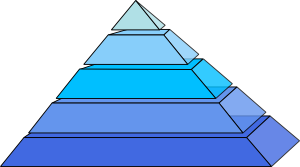
\includegraphics[width=1.1cm]{../Strukturfiler/FIGS/BluePyramid} & \begin{minipage}{\obsl}}{\end{minipage}\\ \end{tabular}\vspace{4mm}\newline}


% = Forudsætning = basis
\newenvironment{basis}{\begin{flushleft} \begin{itshape} }{\end{itshape} \end{flushleft}}


% = Opsummering =
\newenvironment{summary}{\clearpage\pagecolor{sumgul}\section{Opsummering}}{\newpage\pagecolor{white}}











% = Counter
\newcounter{opgavecount}[section]
\setcounter{opgavecount}{0}
\newcounter{spgcount}[opgavecount]
\setcounter{spgcount}{0}
\renewcommand{\thespgcount}{\alph{spgcount})}



% = EXERCISE = (DIVIDER)

\newcommand{\exercisebegin}[1][]{\bigskip\needspace{3\baselineskip}\refstepcounter{opgavecount}\titlegraphic{mingroen}\textcolor{mingroen}{\th{Opgave \theopgavecount \hspace*{1cm} #1}}\medskip\par}

% = QUIZEXERCISE = (DIVIDER)

\newcommand{\quizexercisebegin}[1][]{\bigskip\needspace{3\baselineskip}\refstepcounter{opgavecount}\titlegraphic{mingroen}\textcolor{mingroen}{\th{Quiz-Opgave \theopgavecount \hspace*{1cm} #1}}\medskip\par}

% = QUESTION =

\newenvironment{question}{\refstepcounter{spgcount}\begin{itemize}\item[\thespgcount]}{\end{itemize}\hspace*{\fill}}

% = VINK =

\newenvironment{vink}{\begin{tabular}{m{.9cm}<{\hspace*{2mm}}@{}|m{\obsl}@{}}\hspace*{-4pt}\raggedleft
\includegraphics[width=.9cm]{../Strukturfiler/FIGS/Think} & \begin{minipage}{\obsl}}{\end{minipage}\\ \end{tabular}\medskip\\}
	
% = FACIT =

\newenvironment{facit}{\begin{tabular}{m{.9cm}<{\hspace*{2mm}}@{}|m{\obsl}@{}}\hspace*{-4pt}\raggedleft
\includegraphics[width=.9cm]{../Strukturfiler/FIGS/Check} & \begin{minipage}{\obsl}}{\end{minipage}\\ \end{tabular}\medskip\\}








\newcommand{\afsnit}[1]{\bigskip\th{\titlegraphic{mingroen}\textcolor{mingroen}{#1}} \\ \rule[7pt]{.4\textwidth}{1pt} \vspace*{-2.5mm}\par}

% (DIVIDER):
\newcommand{\ugedagdatotitel}[4]{\pagebreak[4]\section{Semesteruge #1 -- #2 Dag \hspace*{1mm} (#3)} \vspace*{-4mm} \rule[5pt]{\textwidth}{1pt}\vspace*{-2.5mm} \begin{center}\large{\th{#4}}\end{center} \fancyhead[C]{\th{Semesteruge #1}}}

\newenvironment{skema}[1]{\definecolor{shadecolor}{rgb}{0.96,.98, 1.0} \setlength{\FrameSep}{6pt} \renewcommand{\FrameHeightAdjust}{10pt} \vspace*{-4pt}\begin{shaded} \begin{tabular}{#1}}{\end{tabular} \end{shaded} \vspace*{-7pt}}


% ========================

% MAKROER

%\newenvironment{matr}[1][]{\hspace*{-.8mm}\left[\hspace*{-1mm}\begin{array}{#1}}{\end{array}\hspace*{-1mm}\right]\hspace*{-.8mm}}
\newcommand{\bevisslut}{\begin{scriptsize} \begin{flushright} $ \blacksquare $ \end{flushright} \end{scriptsize}}

\newcommand{\tref}[2]{\hyperref[#1]{#2 \ref*{#1}}}
\newcommand{\thref}[2]{\hyperref[#1]{#2}}

\newcommand{\refA}[1]{\colorbox{yellow}{\ref{#1}}}
\newcommand{\hrefA}[2]{\colorbox{yellow}{\href{#1}{#2}}}
\newcommand{\trefA}[2]{\colorbox{yellow}{\hyperref[#1]{#2 \ref*{#1}}}}
\newcommand{\threfA}[2]{\colorbox{yellow}{\hyperref[#1]{#2}}}

\newenvironment{matr}[1]{\hspace*{-.8mm}\begin{bmatrix}\hspace*{-1mm}\begin{array}{#1}}{\end{array}\hspace*{-1mm}\end{bmatrix}\hspace*{-.8mm}}
\newcommand{\transp}{\hspace*{-.6mm}^{\top}}

\newcommand{\maengde}[2]{\left\lbrace \hspace*{-1mm} \begin{array}{c|c} #1 & #2 \end{array} \hspace*{-1mm} \right\rbrace}

\newenvironment{eqnalign}[1]{\setlength{\arraycolsep}{1.3pt}\begin{equation}\begin{array}{#1}}{\end{array}\end{equation}\par}
\newcommand{\eqnl}{\setlength{\arraycolsep}{1.3pt}}

\newcommand{\matind}[3]{{_\mathrm{#1}\mathbf{#2}_\mathrm{#3}}}
\newcommand{\vekind}[2]{{_\mathrm{#1}\mathbf{#2}}}
\newcommand{\jac}[2]{{\mathrm{Jacobi}_\mathbf{#1} (#2)}}
\newcommand{\diver}[2]{{\mathrm{div}\mathbf{#1} (#2)}}
\newcommand{\rot}[1]{{\mathbf{rot}\mathbf{(#1)}}}

\newcommand{\am}{\mathrm{am}}
\newcommand{\gm}{\mathrm{gm}}
\newcommand{\E}{\mathrm{E}}
\newcommand{\Span}{\mathrm{span}}
\newcommand{\mU}{\mathbf{U}}

\newcommand{\ms}{\medskip\\}
\newcommand{\bs}{\bigskip\\}

\newcommand{\mA}{\mathbf{A}}
\newcommand{\mB}{\mathbf{B}}
\newcommand{\mC}{\mathbf{C}}
\newcommand{\mD}{\mathbf{D}}
\newcommand{\mE}{\mathbf{E}}
\newcommand{\mF}{\mathbf{F}}
\newcommand{\mK}{\mathbf{K}}
\newcommand{\mI}{\mathbf{I}}
\newcommand{\mM}{\mathbf{M}}
\newcommand{\mN}{\mathbf{N}}
\newcommand{\mQ}{\mathbf{Q}}
\newcommand{\mT}{\mathbf{T}}
\newcommand{\mV}{\mathbf{V}}
\newcommand{\mW}{\mathbf{W}}
\newcommand{\mX}{\mathbf{X}}
\newcommand{\ma}{\mathbf{a}}
\newcommand{\mb}{\mathbf{b}}
\newcommand{\mc}{\mathbf{c}}
\newcommand{\md}{\mathbf{d}}
\newcommand{\me}{\mathbf{e}}
\newcommand{\mn}{\mathbf{n}}
\newcommand{\mr}{\mathbf{r}}
\newcommand{\mv}{\mathbf{v}}
\newcommand{\mw}{\mathbf{w}}
\newcommand{\mx}{\mathbf{x}}
\newcommand{\mxb}{\mathbf{x_{bet}}}
\newcommand{\my}{\mathbf{y}}
\newcommand{\mz}{\mathbf{z}}
\newcommand{\reel}{\mathbb{R}}
\newcommand{\mL}{\bm{\Lambda}} %Lambda-matrix
\newcommand{\mnul}{\bm{0}}
\newcommand{\trap}[1]{\mathrm{trap}(#1)}
\newcommand{\Det}{\operatorname{Det}}
\newcommand{\adj}{\operatorname{adj}}
\newcommand{\Ar}{\operatorname{Areal}}
\newcommand{\Vol}{\operatorname{Vol}}
\newcommand{\Rum}{\operatorname{Rum}}
\newcommand{\diag}{\operatorname{\bf{diag}}}
\newcommand{\bidiag}{\operatorname{\bf{bidiag}}}
\newcommand{\spanVec}[1]{\mathrm{span}\{#1\}}
\newcommand{\Div}{\operatorname{Div}}
\newcommand{\Rot}{\operatorname{\mathbf{Rot}}}

\newcommand{\Jac}{\operatorname{Jacobi}}
\newcommand{\Tan}{\operatorname{Tan}}
\newcommand{\Ort}{\operatorname{Ort}}
\newcommand{\Flux}{\operatorname{Flux}}
\newcommand{\Cmass}{\operatorname{Cm}}
\newcommand{\Imom}{\operatorname{Im}}
\newcommand{\Pmom}{\operatorname{Pm}}
\newcommand{\IS}{\operatorname{I}}
\newcommand{\IIS}{\operatorname{II}}
\newcommand{\IIIS}{\operatorname{III}}
\newcommand{\Le}{\operatorname{L}}
\newcommand{\app}{\operatorname{app}}
\newcommand{\M}{\operatorname{M}}
\newcommand{\re}{\mathrm{Re}}
\newcommand{\im}{\mathrm{Im}}

\newcommand{\compl}{\mathbb{C}} %de komplekse tal
\newcommand{\e}{\mathrm{e}} %eksponentialfunktionen. lodret 'e', og altså ikke kursiv ligesom andre bogstaver.





% Medialink: SCREEN: (QRcode) + thumbnail image + link på kodenummer (til qr.dtu.dk)
\newcommand{\onlinemedia}[3]{
	\begin{wrapfigure}{r}{3.2cm} 
		\vspace{-30pt} 
		\vspace{#1pt} 
		\begin{flushright} 
			\includegraphics[width=3cm]{qr/#2.png} 
			\tiny 
			\href{http://qr.dtu.dk/#2}{#2: #3}
			\normalsize  
		\end{flushright} 
		\vspace{-10pt} 
	\end{wrapfigure}
}
\newcommand{\onlinemediathumb}[3]{
	\begin{wrapfigure}{r}{3.2cm} 
		\vspace{-30pt} 
		\vspace{#1pt} 
		\begin{flushright} 
			\includegraphics[width=3cm]{qr/#2.png} 
			\includegraphics[width=3cm]{qr/#2_thumb.png} 
			\tiny 
			\href{http://qr.dtu.dk/#2}{#2: #3}
			\normalsize  
		\end{flushright} 
		\vspace{-10pt} 
	\end{wrapfigure}
}



% Index:
\usepackage{makeidx}
\makeindex
\newcommand\ind[2]{\index{#1}\textbf{\textit{\textcolor{black}{#2}}}}

% ###SERVER_EXCLUDE_BEGIN###
\externaldocument[NUID17-]{../../enoten/TN01-Talrum/Talrum}
\externaldocument[NUID1-]{../../enoten/TN02-Ligningssystemer/TNdriver}
\externaldocument[NUID2-]{../../enoten/TN03-Matricer_og_Matrixalgebra/Matricer_og_matrixalgebra}
\externaldocument[NUID3-]{../../enoten/TN04-Kvadratiske_matricer/TNdriver}
\externaldocument[NUID11-]{../../enoten/TN05-Determinanter/Determinanter}
\externaldocument[NUID12-]{../../enoten/TN06-GeometriskeVektorer/GeometriskeVektorer}
\externaldocument[NUID18-]{../../enoten/TN07-Vektorrum/VektorRum}
\externaldocument[NUID21-]{../../enoten/TN08-LinAfbildninger/LinAfbildninger}
\externaldocument[NUID23-]{../../enoten/TN09-Egenvaerdier_og_egenvektorer/TNdriver}
\externaldocument[NUID24-]{../../enoten/TN10-Diagonalisering_med_egenvektorer/TNdriver}
\externaldocument[NUID10-]{../../enoten/TN11-1.ordens_differentialligninger/TNdriver}
\externaldocument[NUID13-]{../../enoten/TN12-1.ordens_differentialligningssystemer/TNdriver}
\externaldocument[NUID14-]{../../enoten/TN13-2.ordens_differentialligninger/TNdriver}
\externaldocument[NUID27-]{../../enoten/TN14-Elemenataere_funktioner/Elementaere_Funktioner}
\externaldocument[NUID28-]{../../enoten/TN15-Funktioner2Variable/Funktioner_To_Variable}
\externaldocument[NUID29-]{../../enoten/TN16-Gradienter_og_Tangentplaner/Gradienter_og_Tangentplaner}
\externaldocument[NUID32-]{../../enoten/TN17-Taylor_formler/Taylor_Formler}
\externaldocument[NUID33-]{../../enoten/TN18-Taylor_2Var/Taylor_2Var}
\externaldocument[NUID34-]{../../enoten/TN19-SymMat/SymmetriskeMatricer}
\externaldocument[NUID35-]{../../enoten/TN20-KegleSnit/Keglesnit}
\externaldocument[NUID36-]{../../enoten/TN21-Riemann_Integral/Riemann_01}
\externaldocument[NUID37-]{../../enoten/TN22-Plan_Int/Plan_Int_01}
\externaldocument[NUID39-]{../../enoten/TN23-Flade_Int/Flade_Rum_Int_01}
\externaldocument[NUID40-]{../../enoten/TN24-Vektorfelter/Vektorfelter_01}
\externaldocument[NUID41-]{../../enoten/TN25-Flux/Flux_02}
\externaldocument[NUID42-]{../../enoten/TN26-Gauss/Gauss_01}
\externaldocument[NUID128-]{../../enoten/TN27-Stokes/Stokes_01}
\externaldocument[NUID43-]{../../enoten/TN29-KomplekseTal/KomplekseTal}

\externaldocument[NUID6-]{../../E-math-opgaver/Opgaver/opgU123}
\externaldocument[NUID19-]{../../E-math-opgaver/Opgaver/opgU45}
\externaldocument[NUID20-]{../../E-math-opgaver/Opgaver/opgU678}
\externaldocument[NUID25-]{../../E-math-opgaver/Opgaver/opgU910SD}
\externaldocument[NUID31-]{../../E-math-opgaver/OpgaverF11-U123/opgF123}
% \externaldocument[NUID9-]{../../E-math-opgaver/Opgaver/Dagsordner E10}
% ###SERVER_EXCLUDE_END###


% Begin document and set alternative chapter title:
\begin{document}
\renewcommand{\chaptername}{eNote}

\setcounter{chapter}{26} %SÆT DETTE TAL TIL 1 MINDRE END DET AKTUELLE TRANSFERNOTE-NUMMER!!

%%%%%%%%%%%%%%%%%%%%%%%%%%%%%%%%%%%%%%%%%%%%%
%%%%%%%%%%%%%%%%%%%%%%%%%%%%%%%%%%%%%%%%%%%%%
%%% HERFRA SKAL DU SKRIVE ELLER INDSÆTTE %%%%
%%% DEN FIL DU ØNSKER %%%%%%%%%%%%%%%%%%%%%%%
%%%%%%%%%%%%%%%%%%%%%%%%%%%%%%%%%%%%%%%%%%%%%
%%%%%%%%%%%%%%%%%%%%%%%%%%%%%%%%%%%%%%%%%%%%%

% REF: TransferNote \ref{TN4-tn4} \nameref{TN4-tn4}
%
% \tref{NUID14-thm.koma}{sætning} \tref{NUID28-tn15}{eNote}
%
%\tref{NUID34-tn19}{eNote} Symmetriske matricer
%\tref{NUID33-tn18}{eNote} Taylor i 2 variable
%
% 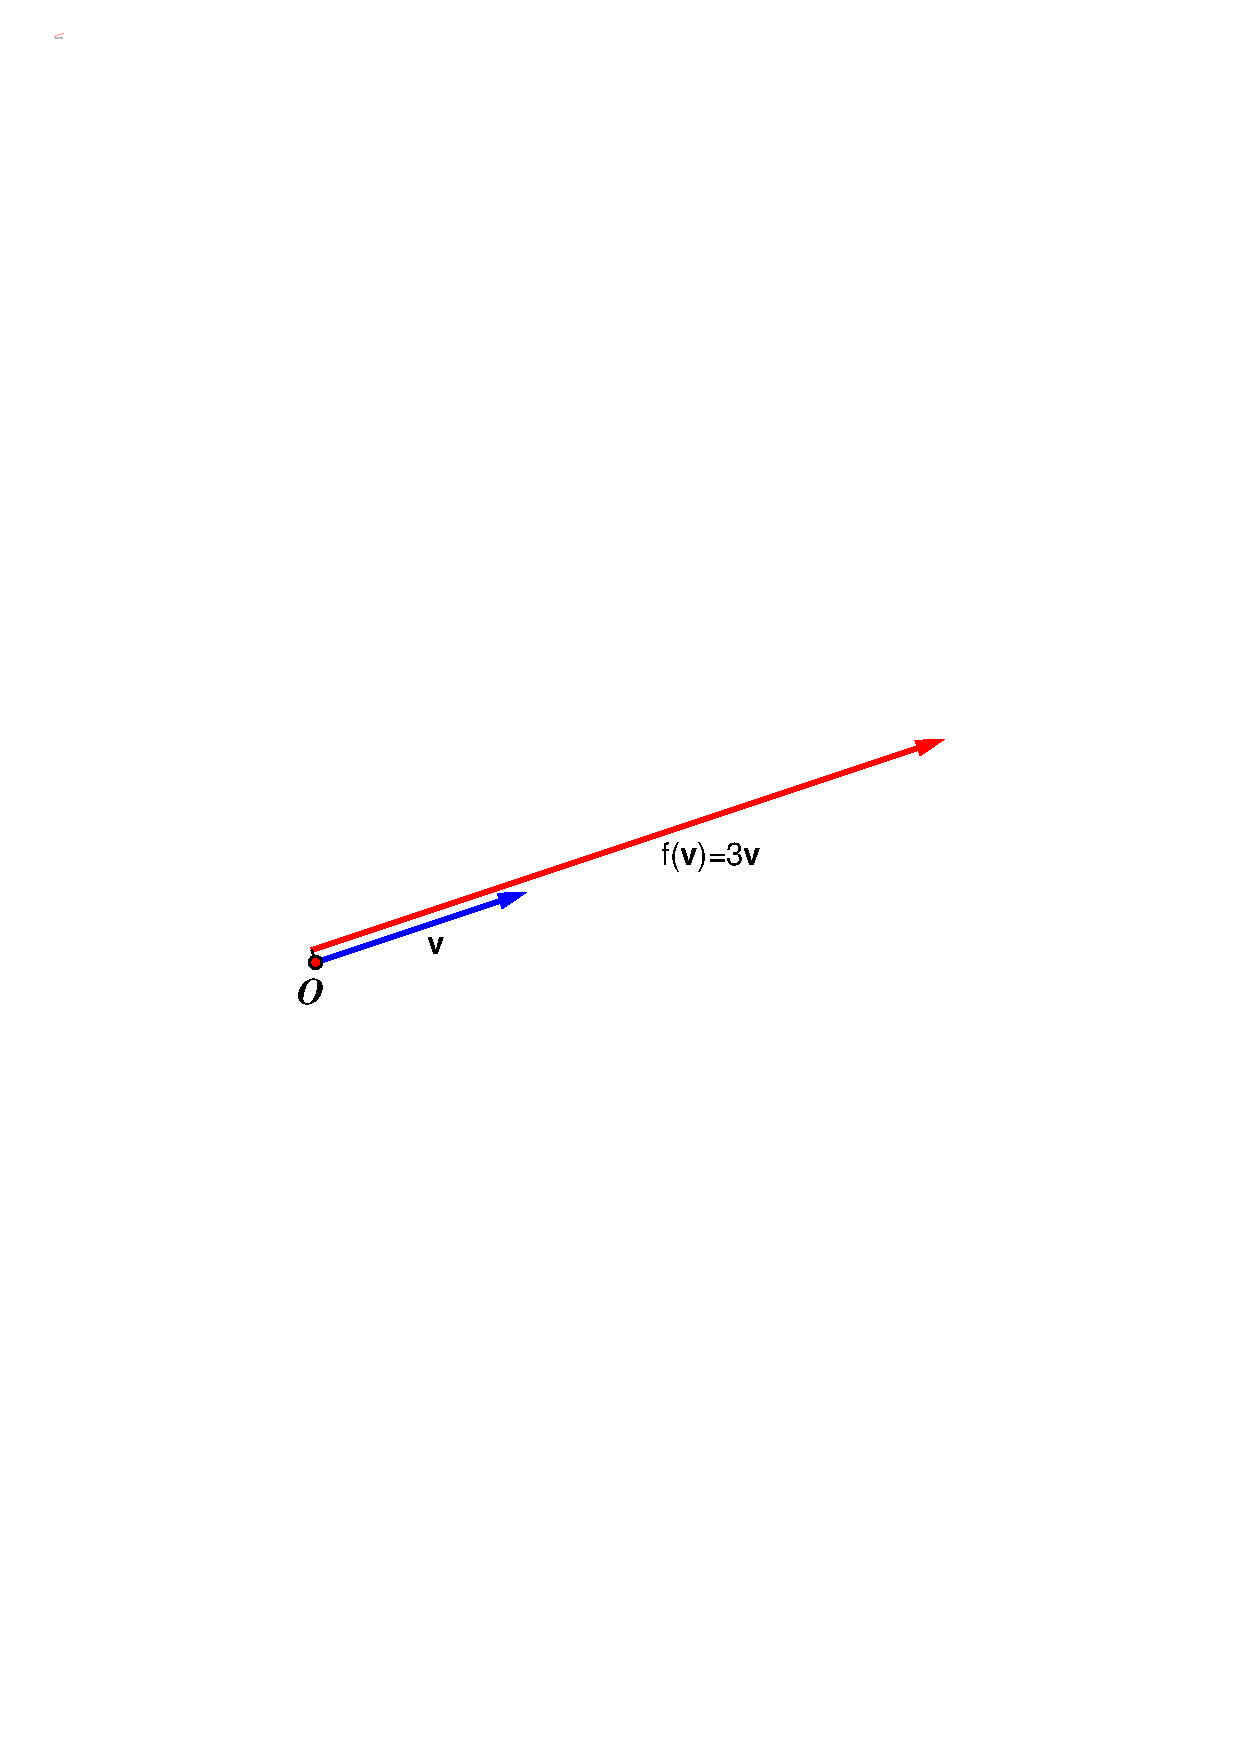
\includegraphics[trim=5cm 12cm 5cm 12cm,width=0.40\textwidth,clip]{skalering.pdf}
%
%\begin{equation}
%\matind vMa \cdot \matind aFa \cdot \matind aMv = \matind vFv \, ,
%\end{equation}
%hvor
%\begin{equation}
%\matind aMv = \begin{matr}{cccc} \vekind av_1 & \vekind av_2 & \cdots & \vekind av_n \end{matr} \quad \mathrm{og} \quad %\matind vFv = \diag(\lambda_1, \lambda_2, \ldots, \lambda_n) \, .
%\end{equation}
%
%$\vekind{e}{F}$
%$\matind{e}{F}{w}$
%
%\href{http://www-groups.dcs.st-and.ac.uk/~history/}{http://www-groups.dcs.st-and.ac.uk/~history/}

%%%%%%%%%%%%%%%%%%%%%%%%%%%%%%%%%%%%%%%%%%%%%%%%%%%
%%%%%%%%%%%%%%%%%%%%%%%%%%%%%%%%%%%%%%%%%%%%%%%%%%%
%%%%%%%%%%%%%%%%%%%%%%%%%%%%%%%%%%%%%%%%%%%%%%%%%%%
%%%%%%%%%%%%%%%%%%%%%%%%%%%%%%%%%%%%%%%%%%%%%%%%%%%

\chapter{Stokes' rotationssætning} \label{tn27}


\begin{basis}
I denne eNote vil vi benytte Gauss' divergenssætning fra \tref{NUID42-tn26}{eNote} til  at motivere, bevise, og illustrere Stokes' sætning, som udtrykker en præcis sammenhæng mellem \emph{rotation} og \emph{cirkulation} af et givet vektorfelt: For enhver glat parametriseret flade $F_{\mathbf{r}}$ er fluxen af rotationen af et glat vektorfelt $\mathbf{V}(x,y,z)$ igennem $F_{\mathbf{r}}$ lig med cirkulationen af vektorfeltet langs randkurven $\partial F$. Som hermed antydet får vi brug for både rum-, flade-, og kurve-integraler samt viden om vektorfelter og deres restriktioner til flader og kurver. Det vil sige, at basismaterialet for nærværende eNote skal findes i en række eNoter: \tref{NUID37-tn22}{eNote} (om plan- og kurve-integraler), \tref{NUID39-tn23}{eNote} (om fladeintegraler), \tref{NUID40-tn24}{eNote} (om vektorfelter), \tref{NUID41-tn25}{eNote} (om tangentielle kurveintegraler ogcirkulationer), og \tref{NUID42-tn26}{eNote} (om flux-beregninger og Gauss' sætning).
\end{basis}


%%%%%%%%%%%%%%%%%%%%%%%%%%%%%%%%%%%%%%%%%%%%%%%%%%%
%%%%%%%%%%%%%%%%%%%%%%%%%%%%%%%%%%%%%%%%%%%%%%%%%%%
%%%%%%%%%%%%%%%%%%%%%%%%%%%%%%%%%%%%%%%%%%%%%%%%%%%
%%%%%%%%%%%%%%%%%%%%%%%%%%%%%%%%%%%%%%%%%%%%%%%%%%%
%%%%%%%%%%%%%%%%%%%%%%%%%%%%%%%%%%%%%%%%%%%%%%%%%%%


%%%%%%%%%%%%%%%%%%%%%%%%%%%%%%%%%%%%%%%%%%%%%%%%%%%
%%%%%%%%%%%%%%%%%%%%%%%%%%%%%%%%%%%%%%%%%%%%%%%%%%%
%%%%%%%%%%%%%%%%%%%%%%%%%%%%%%%%%%%%%%%%%%%%%%%%%%%



\section{Stokes' sætning}  \label{secIntro}


\begin{figure}[h]
\centerline{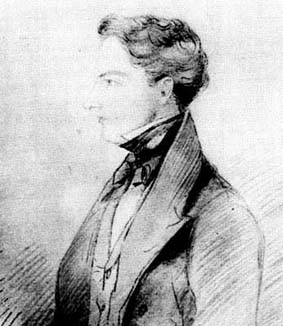
\includegraphics[height=50mm]{FIGS/PERSStokes_4}}
\begin{center}
\caption{\small{George Gabriel Stokes. Se \href{http://www-history.mcs.st-and.ac.uk/Mathematicians/Stokes.html}{Biografi}.}} \label{figStokes}
\end{center}
\end{figure}



{Stokes' sætning} er en af de mest elegante og mest
benyttede resultater fra analysen af vektorfelter
i rummet. Sætningen har ligesom Gauss'
divergenssætning mangfoldige anvendelser - f.eks.
i fluid mekanik og i elektromagnetisme. \\

Her er et
citat som fortæller lidt om
historien bag resultatet:\\

\begin{quote}
The history of Stokes' Theorem is clear but very
complicated. It was first given by Stokes without
proof - as was necessary since it was given as
an examination question for the Smith's Prize
Examination of that year [at Cambridge in 1854]!
Among the candidates for the prize was Maxwell,
who later traced to Stokes the origin of the
theorem, which by 1870 was frequently used. On
this see George Gabriel Stokes, {\em{Mathematical
and Physical Papers}}, vol. V (Cambridge,
England, 1905), 320--321. See also the important
historical footnote which indicates that Kelvin
in a letter of 1850 was the first who actually
stated the theorem, although others as Amp\'{e}re
had employed "the same kind of analysis ... in
particular cases."

\begin{flushright}
M. J. Crowe, [A history of vector analysis, 1967],  s. 147.
\end{flushright}
\end{quote}


\begin{figure}[h]
\centerline{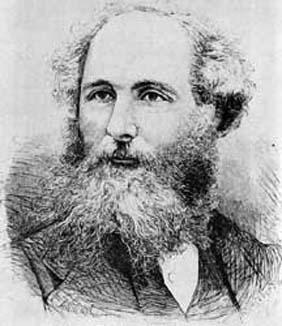
\includegraphics[height=50mm]{FIGS/PERSMaxwell_8}\qquad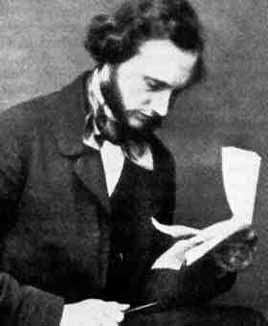
\includegraphics[height=50mm]{FIGS/Thomson01}\qquad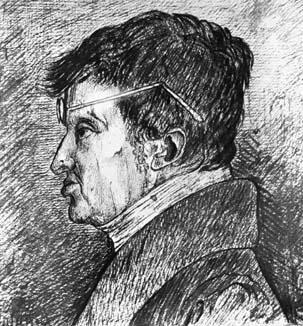
\includegraphics[height=50mm]{FIGS/Ampere_9}}
\begin{center}
\caption{\small{James Clerk Maxwell \href{http://www-history.mcs.st-and.ac.uk/Mathematicians/Maxwell.html}{(Biografi)},
William Thomson (Lord Kelvin)  \href{http://www-history.mcs.st-and.ac.uk/Mathematicians/Thomson.html}{(Biografi)}, og
Andr\`{e}-Marie Amp\'{e}re  \href{http://www-history.mcs.st-and.ac.uk/Mathematicians/Ampere.html}{(Biografi)}.}} \label{figStokesKelvinAmpere}
\end{center}
\end{figure}




Som antydet er Stokes' resultat af
samme kaliber som Gauss' divergens-sætning. De er
begge to medlemmer af en 'familie' af resultater,
hvor hovedideen er at omskrive et integral over
et område til en andet integral over områdets
rand - altså så at sige 'skubbe integrationen ud
på randen'. Det ældste medlem af den familie er
Integralregningens fundamental-sætning, jvf. \tref{NUID36-thmAnalyseFundamental}{sætning} \tref{NUID36-tn21}{eNote}
som vi gentager her med følgende formulering:

\begin{theorem}[Integralregningens fundamentalsætning]  \label{thmFundamCalc}
Lad $f(u)$ betegne en kontinuert funktion på
$\mathbb{R}$. Så er følgende funktion
differentiabel
\begin{equation} \label{eqAP}
A(x) \, = \,  \int_{0}^{x}\,f(u)\, du \qquad
\textrm{med}\qquad A'(x) \, = \, f(x) \quad .
\end{equation}
Hvis $F(x)$ er en (anden) funktion, som  opfylder
$F'(x) \, = \, f(x)$, så er
\begin{equation} \label{eqIntFundam}
\int_{a}^{b}\,f(u)\,du \, = \, F(b) - F(a) \quad
.
\end{equation}
\end{theorem}

Her er nu formuleringen af {Stokes' sætning}:

\begin{theorem}[Stokes' sætning] \label{thmStokes}
Lad $F_{\bf{r}}$ betegne en glat parametriseret flade
med randkurven $\partial F_{\bf{r}}$ og
en\-heds\--nor\-mal\-vek\-tor\-felt
$\,{\bf{n}}_{F}$ og lad ${\bf{V}}$ være et glat
vektorfelt i $\mathbb{R}^{3}$. Så gælder
\begin{equation} \label{eqStokes}
\int_{F}\, \Rot({\bf{V}})\bm{\cdot} {\bf{n}}_{F} \,
\,d\mu \, = \, \int_{\partial F} \, {\bf{V}}
\bm{\cdot} {\bf{e}}_{\partial F} \, d\mu \quad .
\end{equation}
Ved beregning af højresiden skal orienteringen
(givet ved retningen af enheds-tangent-vektorfeltet $\, {\bf{e}}_{\partial F}\,$) af randen vælges
således at krydsproduktet  ${\bf{e}}_{\partial F}
\times {\bf{n}}_{F}$ peger væk fra fladen langs
med randen.
\end{theorem}

\begin{think}
Stokes' sætning udtrykker altså -- ligesom (\ref{eqIntFundam}) -- at et indre integral (her på et fladestykke) kan udtrykkes som et rand-integral (langs fladestykkets rand). \\
Stokes' sætning kan også formuleres som følger, idet vi henviser til
definitionerne af flux og cirkulation i henholdsvis \tref{NUID42-tn26}{eNote} og \tref{NUID41-tn25}{eNote}:
\begin{equation}
\Flux(\Rot(\mathbf{V}), F_{\mathbf{r}}) = \operatorname{Cirk}(\mathbf{V}, \partial F) \quad .
\end{equation}
Det vil sige: Fluxen af \emph{rotationen af} vektorfeltet $\mathbf{V}$ igennem fladen $F_{\mathbf{r}}$ er lig med \emph{cirkulationen} af vektorfeltet
langs fladestykkets lukkede randkurve  $\partial F$.
\end{think}

\begin{aha}
Læg mærke til, at hvis $F_{\mathbf{r}}$ er \emph{hele} overfladen af et rumligt område, så er $\partial F = \emptyset$, og derfor følger det af Stokes' sætning at
\begin{equation}
\Flux(\Rot(\mathbf{V}), F_{\mathbf{r}}) = 0
\end{equation}
i overensstemmelse med den følgesætning fra Gauss' divergenssætning som er nævnt i \tref{NUID42-CorTotFlux0}{sætning} i \tref{NUID42-tn26}{eNote}.
\end{aha}


%%%%%%%%%%%%%%%%%%%%%%%%%%%%%%%%%%%%%%%%%%%%%%%%%%%%%%%%%%%%%%%%%%%%%%%%%%
\section{Motivering af -- og et bevis for --  Stokes' sætning } \label{secBridge}

Vi får brug for følgende resultat, som også er nævnt i \tref{NUID40-secBridge}{afsnit} i \tref{NUID40-tn24}{eNote}:

\begin{theorem}\label{exerGaussVgrad}
Lad $\,{\bf{V}}(x,y,z)\,$ og
$\,{\bf{W}}(x,y,z)\,$ betegne to vektorfelter i
$\mathbb{R}^{3}$. Så gælder følgende identitet
\begin{equation}
\Div({\bf{V}}\times {\bf{W}}) \, = \,
\Rot({\bf{V}})\bm{\cdot} {\bf{W}} - {\bf{V}}\bm{\cdot}
\Rot({\bf{W}}) \quad .
\end{equation}
Specielt har vi derfor: Hvis  $\,{\bf{W}}$ er et
gradient-vektorfelt for en funktion $\psi(x,y,z)$
i $\mathbb{R}^{3}$, dvs.  $\,{\bf{W}} \, = \,
\bm{\nabla}(\psi)\,$, så får vi fra $\,\Rot (
\bm{\nabla}(\psi) ) \, = \, {\bf{0}}\,$:
\begin{equation}\label{eqRotDivGrad}
\Div({\bf{V}}\times \bm{\nabla}(\psi)) =
\Rot({\bf{V}})\bm{\cdot}\bm{\nabla}(\psi) \quad .
\end{equation}
\end{theorem}

Ved at bruge Gauss' divergens-sætning (\tref{NUID42-thmGauss}{sætning} \tref{NUID42-tn26}{eNote}) i forbindelse med (\ref{eqRotDivGrad}) får vi direkte et interessant resultat om
integraler over rumlige områder således:

\begin{theorem}[En konsekvens af Gauss' divergenssætning] \label{thmGaussStokes}
Lad $\,\psi(x,y,z)\,$ betegne en glat funktion og
${\bf{V}}(x,y,z)\,$ et glat vektorfelt i
$\mathbb{R}^{3}$. Lad $\Omega$ være et rumligt
område med randen $\partial \Omega$ og udadrettet
enheds-normalvektorfelt $\,{\bf{n}}_{\partial
\Omega}\,$ på $\partial \Omega$. \\

Så har vi direkte fra Gauss' \tref{NUID42-thmGauss}{sætning}:
\begin{equation} \label{eqIntDivRotA}
\int_{\Omega}\, \Div({\bf{V}}\times
\bm{\nabla}(\psi))\, d\mu \,  = \, \int_{\partial
\Omega}\,  \left({\bf{V}}\times
\bm{\nabla}(\psi)\right)\bm{\cdot} {\bf{n}}_{\partial
\Omega} \,\, d\mu \quad .
\end{equation}
Ved brug af  (\ref{eqRotDivGrad}) har vi derfor
også
\begin{equation} \label{eqIntDivRotB}
\int_{\Omega}\, \Rot({\bf{V}})\bm{\cdot}\bm{\nabla}(\psi)\,
d\mu \,  = \, \int_{\partial \Omega}\,
\left({\bf{n}}_{\partial \Omega}\, \times
{\bf{V}}\right) \bm{\cdot} \bm{\nabla}(\psi)
 \, \,d\mu \quad .
\end{equation}
\end{theorem}

\begin{think}
På højresiden i ligning (\ref{eqIntDivRotB}) har vi
benyttet, at rumproduktet $\,[{\bf{a}} {\bf{b}}
{\bf{c}}\,]\, = \, ({\bf{a}} \times {\bf{b}})
\bm{\cdot} {\bf{c}}\, $  af tre vektorer ${\bf{a}}$,
${\bf{b}}$, og ${\bf{c}}$ tilfredsstiller
følgende identiteter (hvoraf vi har brugt den
første):
\begin{equation}
[{\bf{a}} {\bf{b}} {\bf{c}}\,]\, = \, [{\bf{c}}
{\bf{a}} {\bf{b}}\,] \, = \, [{\bf{b}} {\bf{c}}
{\bf{a}}\,] \, = \, - [{\bf{b}} {\bf{a}}
{\bf{c}}\,]\, = \, -[{\bf{c}} {\bf{b}}
{\bf{a}}\,] \, = \, -[{\bf{a}} {\bf{c}}
{\bf{b}}\,] \quad .
\end{equation}
\end{think}


Specielt får vi den totale rotationsvektor af
vektorfeltet ${\bf{V}}$ i $\Omega\,$ således:

\begin{corollary}[Totale rotation i et rumligt område]\label{lemmaTotalRot}
Lad $\Omega$ være et rumligt
område med randen $\partial \Omega$ og udadrettet
enheds-normalvektorfelt $\,{\bf{n}}_{\partial
\Omega}\,$ på $\partial \Omega$. Så gælder for ethvert glat vektorfelt $\mathbf{V}(x,y,z)$:
\begin{equation} \label{eqVridning}
\int_{\Omega}\, \Rot({\bf{V}})\, d\mu \,  = \,
\int_{\partial \Omega}\, {\bf{n}}_{\partial
\Omega}\, \times {\bf{V}}
 \, \,d\mu \quad .
\end{equation}
\end{corollary}

\begin{bevis}
Dette følger direkte af  (\ref{eqIntDivRotB}) ved
at vælge, skiftevis, $\psi(x,y,z) \, = \, x\,$,
$\psi(x,y,z) \, = \, y\,$, og $\psi(x,y,z) \, =
\, z\,$, således at $\bm{\nabla}(\psi)$ er henholdsvis
$(1,0,0)$, $(0,1,0)$, og $(0,0,1)$.
\end{bevis}

Højresiden af ligningen (\ref{eqVridning}) vil vi
tillade os at kalde {\em{den totale {vridning}}} af
fladen $\partial \Omega$ med vektorfeltet
$\bf{V}$ med hensyn til normalvektorfeltet
${\bf{n}}_{\partial \Omega}$ og iøvrigt betegne
denne vektor med ${\operatorname{\bf{Vrid}}}({\bf{V}},
\partial \Omega)$ således:

\begin{definition}[Vridning]\label{defVridning}
Lad $F_{\mathbf{r}}$ betegne en glat flade i rummet med standard enheds-normalvetorfelt $\mathbf{n}_{F}$, og lad $\mathbf{V}(x,y,z)$ være et glat vektorfelt. Så definerer vi vridningen af $F_{\mathbf{r}}$ med vektorfeltet $\mathbf{V}(x,y,z)$ på følgende måde:
\begin{equation}
{\operatorname{\bf{Vrid}}}({\bf{V}},
F_{\mathbf{r}}) \, = \, \int_{F_{\mathbf{r}}}\, {\bf{n}}_{F}\, \times {\bf{V}}
 \, \,d\mu  \quad .
\end{equation}
\end{definition}

Generelt er den totale rotation af et givet vektorfelt i et rumligt område (også kaldet
'total vorticity' i fluid mekanik) altså --  via \ref{lemmaTotalRot} -- lig
med vridningen af områdets overflade med vektorfeltet. Dette minder meget om  Gauss' tilsvarende
identitet for den totale divergens af et glat vektorfelt, \tref{NUID42-thmGauss}{sætning}: Den totale divergens af vektorfeltet i et
område er lig med fluxen af vektorfeltet ud igennem overfladen
af området. \\

I lighed med \tref{NUID42-thmDivGeom}{sætning}
har vi da også følgende tolkning og konstruktion
af rotationsvektoren i et givet punkt:

\begin{theorem} \label{thmRotGeom}
Rotationen af et vektorfelt udtrykker {\em{den
{volumen-relative lokale vridning} af overfladen}}
for vektorfeltet i følgende forstand: Lad
$K_{\rho}$ betegne en massiv kugle med radius
$\rho$ og centrum i punktet $(x_{0}, y_{0},
z_{0})$. Så gælder:
\begin{equation} \label{eqVridRot}
\lim_{\rho \to 0}\left(
\frac{1}{\Vol(K_{\rho})}\,{\operatorname{\bf{Vrid}}}({\bf{V}},
\partial K_{\rho})\right) \, =  \,
\Rot({\bf{V}})(x_{0}, y_{0}, z_{0}) \quad .
\end{equation}
\end{theorem}

\begin{think}
Sætning \ref{thmRotGeom} indses på samme måde som for den
analoge identitet for divergensen.
Vektorfeltet udvikles til første orden med
udviklingspunkt $p$ og indsættes i
vridningsudtrykket, hvorefter følgende identiteter benyttes:

\begin{equation} \label{eqKugleintegraler}
\begin{aligned}
&\int_{\partial K_{\rho}}\,x \,\,d\mu \, = \,
\int_{\partial K_{\rho}}\,y \,\,d\mu \, = \,
\int_{\partial K_{\rho}}\,z \,\,d\mu \, = \,0 \quad , \\
&\int_{\partial K_{\rho}}\,x^{2}\,\, d\mu \, = \,
\int_{\partial K_{\rho}}\,y^{2}\,\, d\mu \, = \,
\int_{\partial K_{\rho}}\,z^{2}\,\, d\mu \, = \, (4\,\pi/3)\,\rho^{4}\, = \, \rho\,\Vol(K_{\rho})\quad , \\
& \int_{\partial K_{\rho}}\,x\,y \,\,d\mu \, = \,
\int_{\partial K_{\rho}}\,x\,z \,\,d\mu \, =
\,\int_{\partial K_{\rho}}\,z\,y \,\,d\mu \, =
\,0 \quad .
\end{aligned}
\end{equation}

De eneste
partielle afledede af vektorfeltets
koordinatfunktioner, der ikke integreres væk, er
præcis dem, der optræder i rotationsvektoren
$\,\Rot({\bf{V}})\,$ når denne evalueres i $p$.
Prøv det!
\end{think}

\begin{example}[Lokal vridning af kugleflade giver rotationsvektoren]
Vi ser på et roterende vektorfelt
${\bf{V}}(x,y,z)\, = \, (-y, x, 1)$. Dette felt har den konstante
rotation $\,\Rot({\bf{V}})\, = \, (0, 0, 2)\,$. Vi vil vise, hvordan
$\operatorname{\bf{Vrid}}({\bf{V}},
\partial K_{\rho})$ netop giver denne rotation i
punktet $(0,0,0)$. Lad altså $\,K_{\rho}\,$
betegne den kugleflade, der har radius
$\,\rho\,$, centrum i $(0,0,0)$, og overflade
$\partial K_{\rho}$ med udadrettet
normalvektorfelt ${\bf{n}}\, = \,
\frac{1}{\rho}(x,y,z)$. Så er
$$
\begin{aligned}
\operatorname{\bf{Vrid}}({\bf{V}}, \partial K_{\rho}) \, = \,
&\int_{\partial K_{\rho}}\, {\bf{n}_{\partial K}}\times
{\bf{V}} \, \, d\mu \,
\\ = \,  &\frac{1}{\rho}\,\int_{\partial K_{\rho}}\, (x, y, z) \times (-y, x, 1 ) \, \, d\mu \, \\ = \,
&\frac{1}{\rho}\,\int_{\partial K_{\rho}}\, (\,y
- x\,z\, , \,\, -x - y\,z\, , \,\, x^{2} +
y^{2}\,) \, \, d\mu \, \\ = \, &\qquad (0, \,
0,\, 2\,\Vol(K_{\rho})\,) \, \\ = \, &\qquad
\Vol(K_{\rho})\,\Rot({\bf{V}})(0,0,0) \quad ,
\end{aligned}
$$
i overensstemmelse med sætning \ref{thmRotGeom}.
\end{example}

\begin{aha}
I mere komplicerede tilfælde kan den totale
vridning af en flade med et givet vektorfelt
beregnes med Maple. Hvis den aktuelle
flade er randoverfladen af et givet rumligt
område kan vridningen også beregnes som integralet af det tilhørende  rotationsvektorfelt over det rumlige område. Derved muliggøres
naturligvis også konkrete eftervisninger af
ligning (\ref{eqVridning}).
\end{aha}



%%%%%%%%%%%%%%%%%%%%%%%%%%%%%%%%%%%%%%%%%%%%%%%%%%%%%%%%%%%%%%%%%%%%%%%%%%
%%%%%%%%%%%%%%%%%%%%%%%%%%%%%%%%%%%%%%%%%%%%%%%%%%%%%%%%%%%%%%%%%%%%%%%%%%
%%%%%%%%%%%%%%%%%%%%%%%%%%%%%%%%%%%%%%%%%%%%%%%%%%%%%%%%%%%%%%%%%%%%%%%%%%
%%%%%%%%%%%%%%%%%%%%%%%%%%%%%%%%%%%%%%%%%%%%%%%%%%%%%%%%%%%%%%%%%%%%%%%%%%

\subsection{Fladen, randen, og normal-vektorfeltet} \label{secSurf}
De flader, der betragtes i Stokes' sætning er
parametriserede på sædvanlig vis:
\begin{equation}
F_{\bf{r}}: \qquad  {\bf{r}}(u,v) \, = \,
(x(u,v), y(u,v), z(u,v)) \in \mathbb{R}^{3} \quad ,
\end{equation}
hvor
\begin{equation}
(u,v) \in D\, = \, [a, b]\times[c, d]
\subset \mathbb{R}^{2} \quad.
\end{equation}

Randen $\partial F_{\bf{r}}$ af $F_{\bf{r}}$
fremkommer ved at bruge vektorfunktionen $\bf{r}$
på de 4 rette linjestykker, der udgør randen
$\partial D$ af det rektangulære parameterområde
$D\, = \, [a, b]\times[c, d]$. Vi parametriserer
hele $\partial D$ på \'{e}n gang ved hjælp af en
parameter $\theta$ og en vektor-funktion
$\bf{d}$:
$$
\partial D: \qquad  {\bf{d}}(\theta) \, = \, (u(\theta), v(\theta)) \in
\partial D \subset \mathbb{R}^{2} \,\, , \,\, \theta \in I \subset \mathbb{R} \quad,
$$
hvor $u(\theta)$ og $v(\theta)$ kun er stykkevis
differentiable funktioner af $\theta$. De kan
f.eks. vælges som lineære funktioner af $\theta$
for hvert enkelt  af de 4 linjestykker der udgør
$\partial D$.

Randen af $F_{\bf{r}}$ er så
$$
\partial F_{\bf{r}}: \qquad  {\bf{b}}(\theta)\,
= \,{\bf{r}}({\bf{d}}(\theta)) \, = \,
{\bf{r}}(u(\theta), v(\theta)) \in
\mathbb{R}^{3}\,\, , \,\, \theta \in I \subset
\mathbb{R} \quad.
$$

Jacobi-funktionerne for ${\bf{r}}$ og ${\bf{b}}$
er henholdsvis:
\begin{equation}
\Jac_{{\bf{r}}}(u,v) \, = \, \Vert
{\bf{r}}'_{u}\times {\bf{r}}'_{v} \Vert  \quad ,
\quad \textrm{og}
\end{equation}
\begin{equation}
\Jac_{{\bf{b}}}(\theta) \, = \,  \Vert
{\bf{b}}'_{\theta} \Vert \quad .
\end{equation}
Regulariteten af  ${\bf{r}}$ giver
$$
\Jac_{{\bf{r}}}(u,v)\, > \, 0 \quad \textrm{for
all} \quad (u,v) \in D\quad .
$$
Enheds-normalvektorfeltet langs  $F_{\bf{r}}$ er
tilsvarende ${\bf{n}}_{F}\, = \, {\bf{n}}(u,v)$:
\begin{equation}
{\bf{n}}(u,v) \, = \, \frac{{\bf{r}}'_{u}\times
{\bf{r}}'_{v}}{\Vert {\bf{r}}'_{u}\times
{\bf{r}}'_{v}  \Vert} \quad \textrm{for alle}
\quad (u,v) \in D\quad .
\end{equation}

%%%%%%%%%%%%%%%%%%%%%%%%%%%%%%%%%%%%%%%%%%%%%%%%%%%%%%%%%%%%%%%%%%%%%%%%%%
\subsection{Tubulære skaller og en afstandsfunktion} \label{secShell}

Vi definerer {\em{den {tubulære skal} med tykkelse
$t$ ud fra $F_{\bf{r}}$}} som følgende område i
$\mathbb{R}^{3}$:
\begin{equation} \label{eqOmegaT}
 \Omega_{t}: \quad
{\bf{R}}(u,v,w)\, = \, {\bf{r}}(u,v) +
w\,{\bf{n}}(u,v)  \,\, , \,\, (u,v) \in D \,\, ,
\,\, w \in [0, t] \,\, .
\end{equation}
Specielt er  {\em{fladen}} $F_{\bf{r}}$ netop
basis-fladen for skallen og fås ved at bruge
afbildningen ${\bf{R}}$ på $D$ (hvor $w\, = \,
0$):
\begin{equation}
F_{0}\, = \, F_{\bf{R}}(0) \, = \, F_{\bf{r}} \quad :
\quad {\bf{r}}(u,v) \, = \, {\bf{R}}(u,v,0)\,\,
, \,\, (u,v) \in D \quad.
\end{equation}
Tilsvarende får vi, for $w\,=\,t$, top-fladen
af skallen.
Den er parametriseret således:
\begin{equation}
F_{t}\, = \, F_{\bf{R}}(t) \, = \, F_{\bf{\widehat{r}}} \quad :
\quad {\bf{\widehat{r}}}(u,v) \, = \, {\bf{R}}(u,v,t)\,\,
, \,\, (u,v) \in D \quad.
\end{equation}









%%%%%%%%%%%%%%%%%%%%%%%%%%%%%%%%%%%%%%%%%%%%%%%%%%%%%%%%%%%%%

\begin{figure}[h]
\centerline{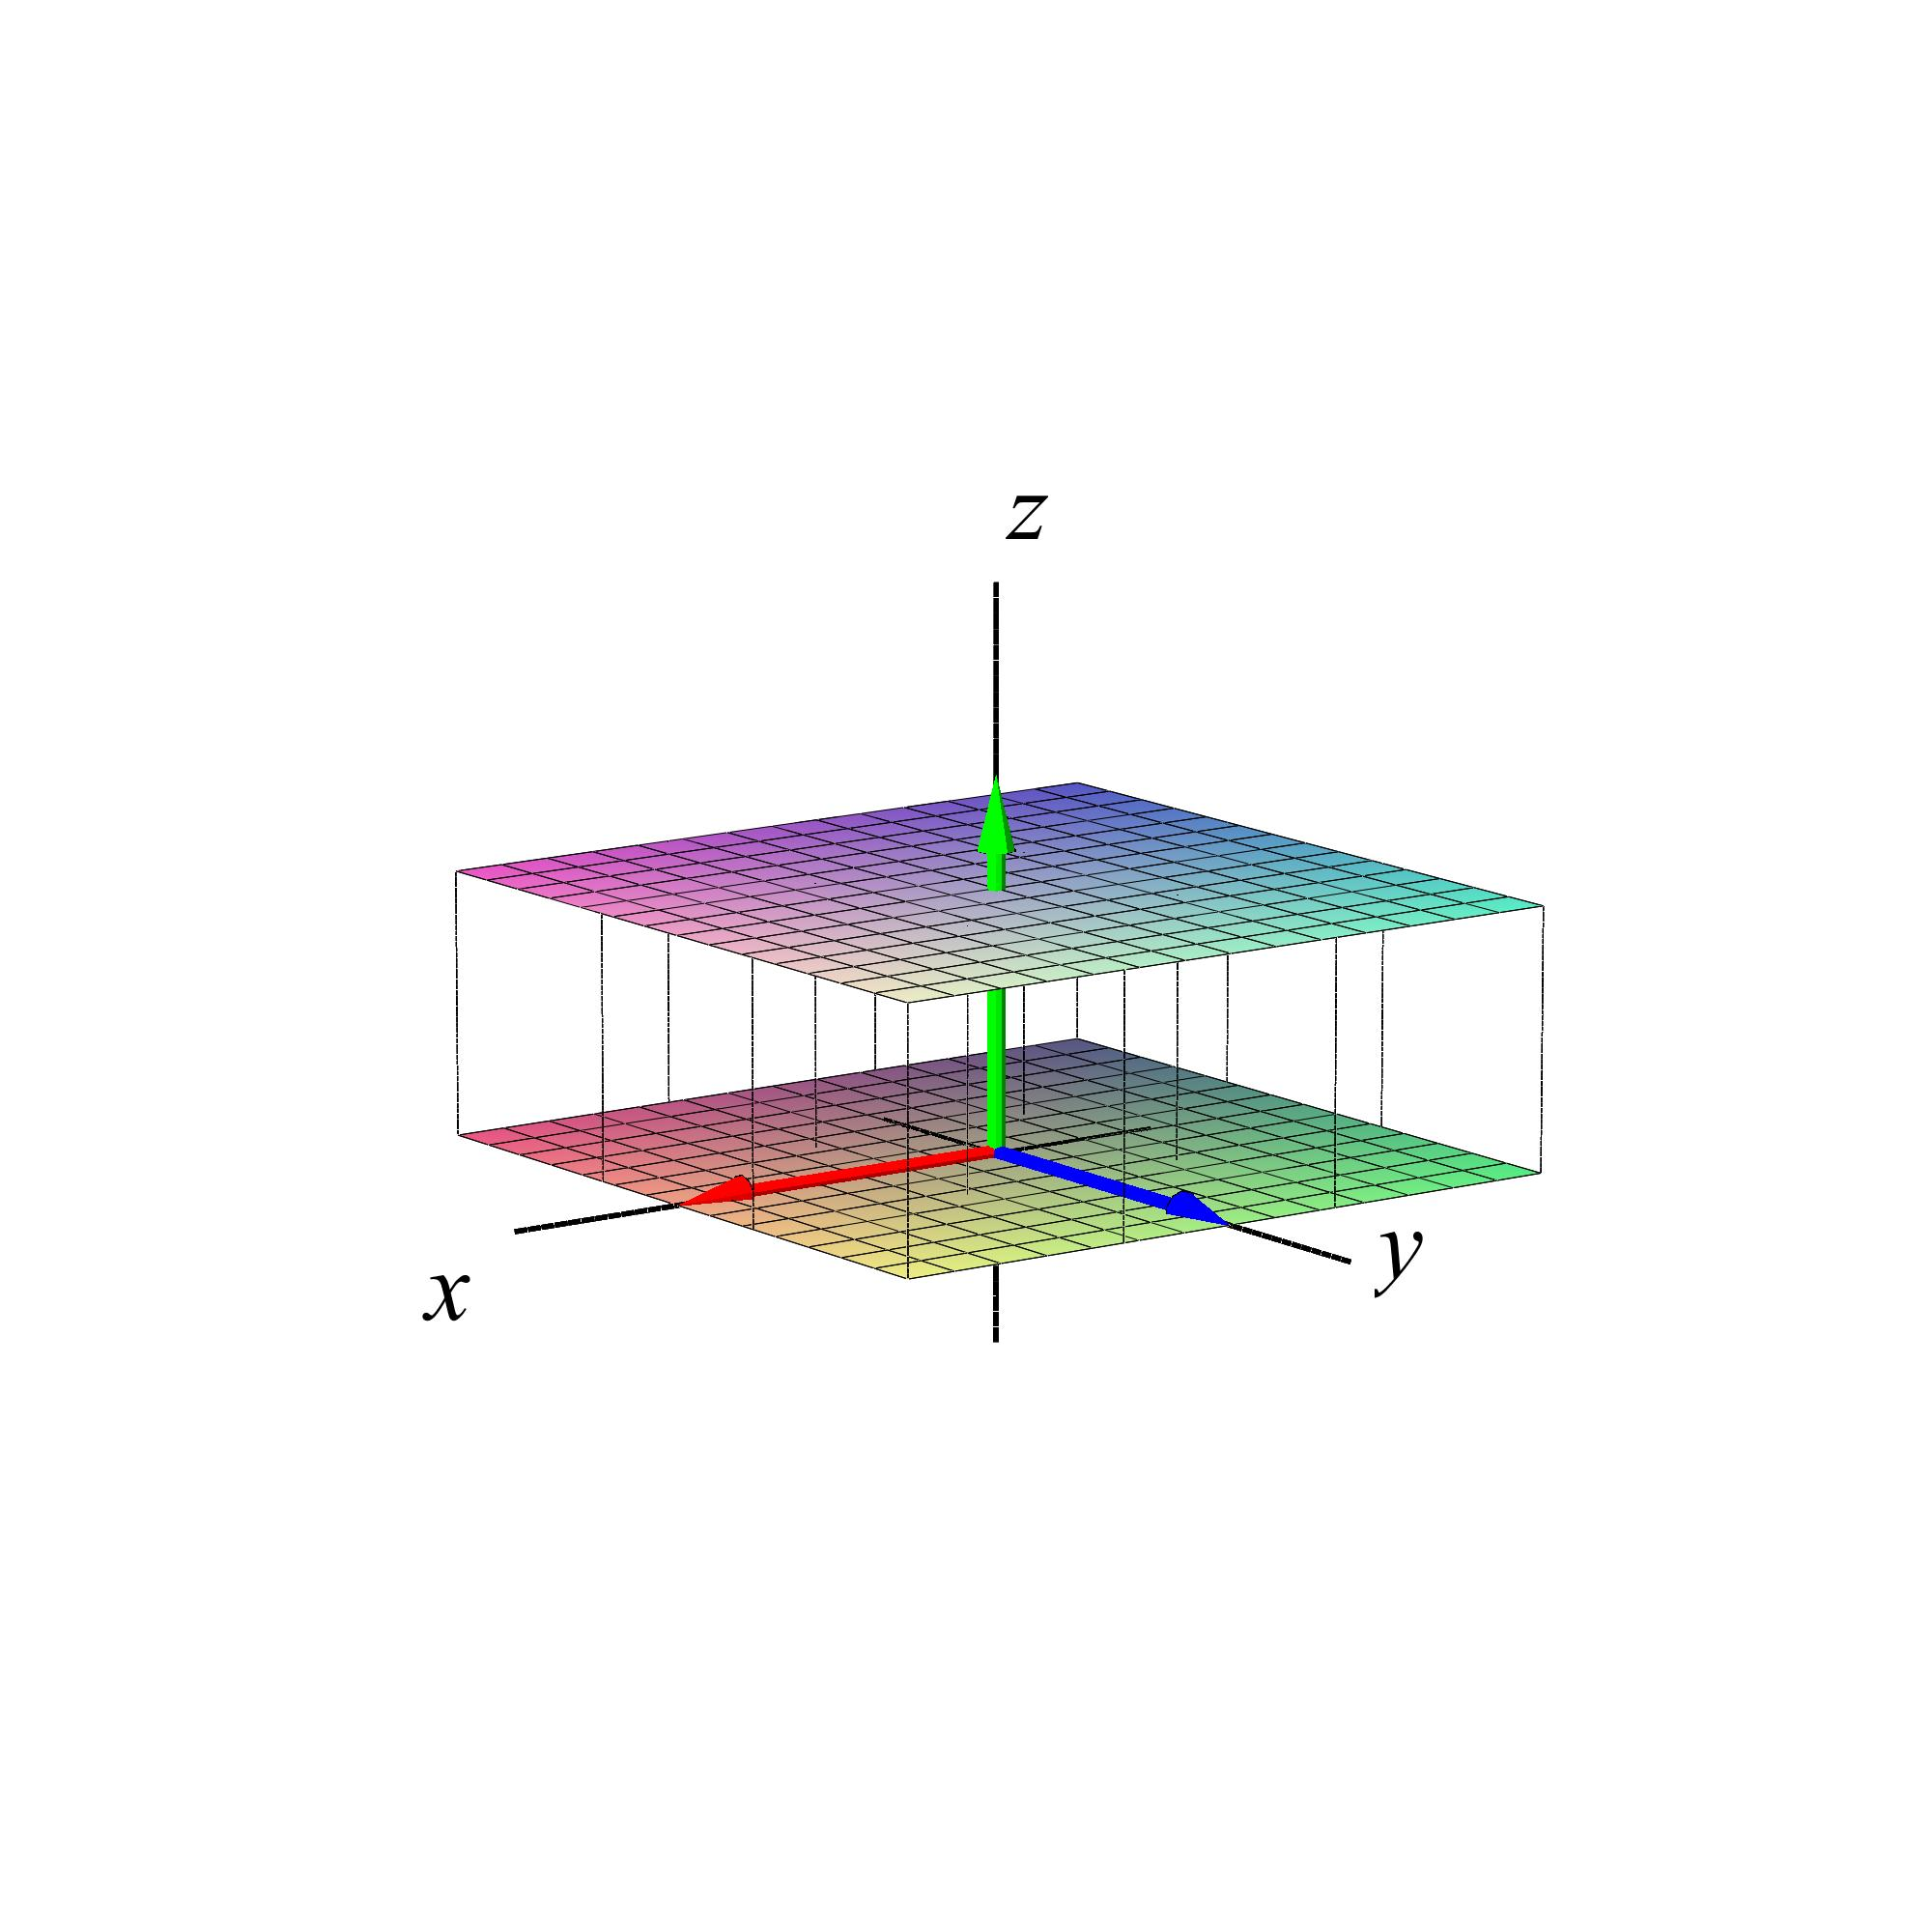
\includegraphics[height=70mm]{FIGS/plotNormalKvadratFlow} 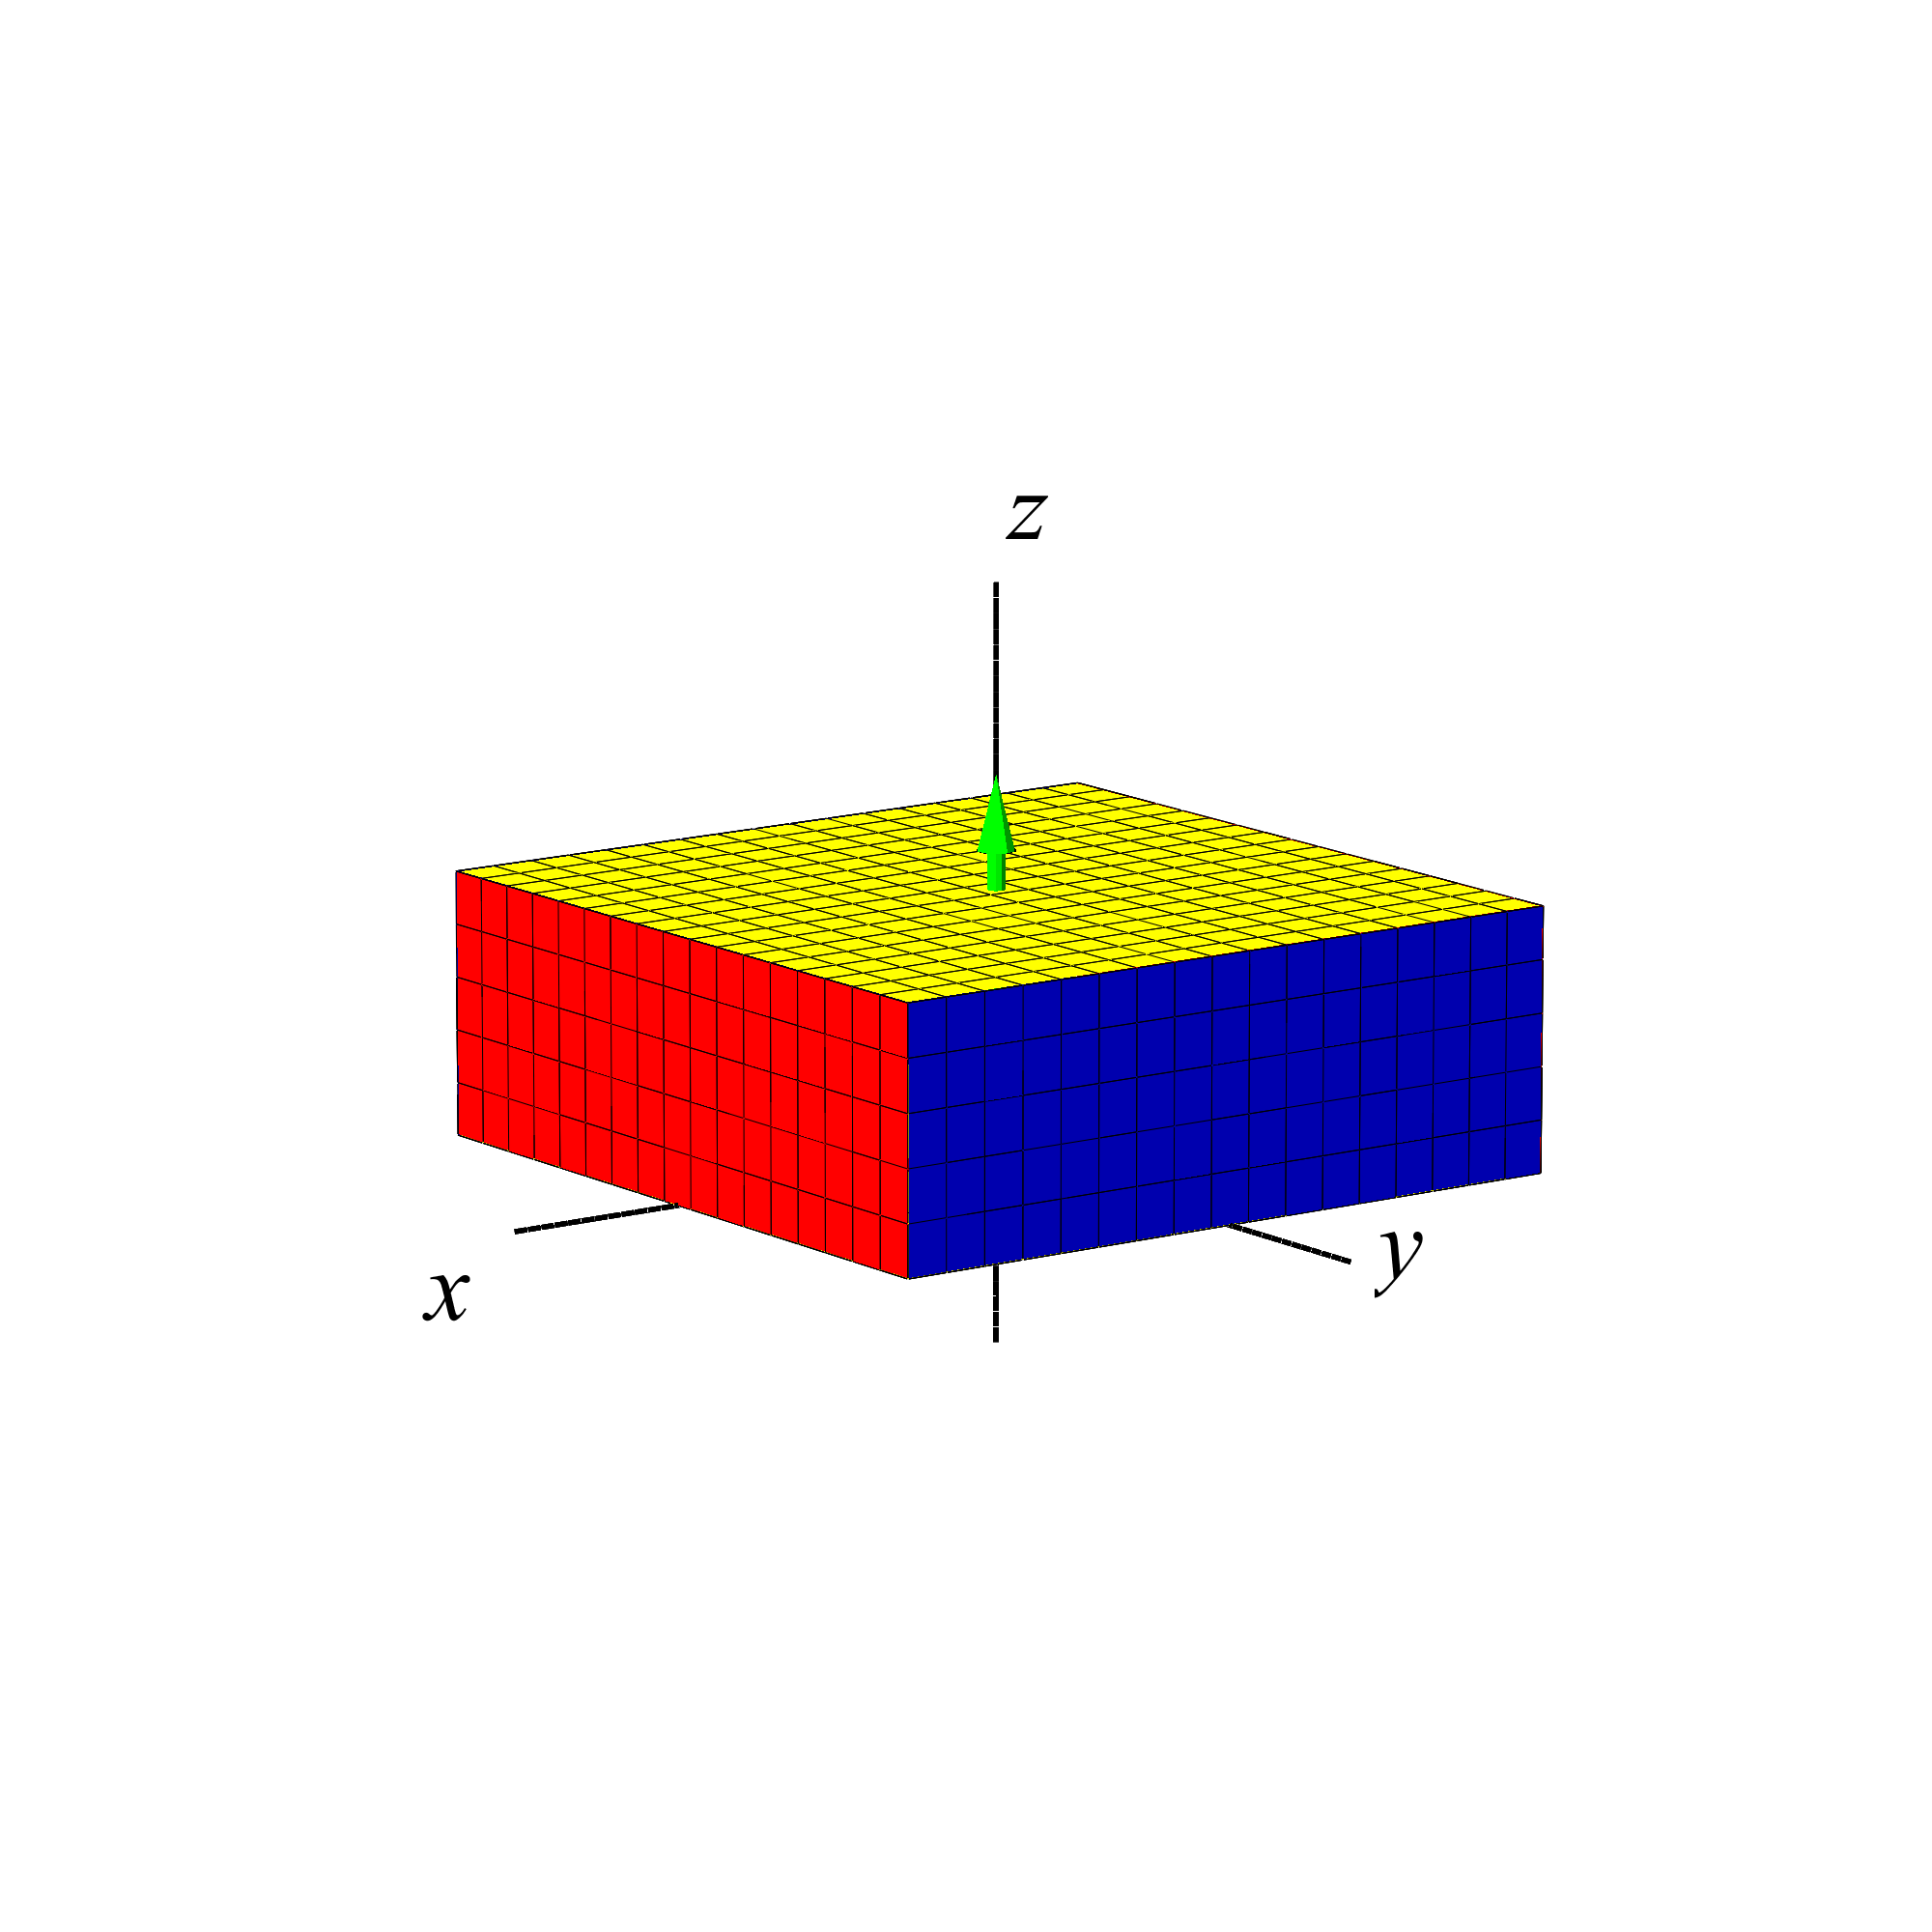
\includegraphics[height=70mm]{FIGS/plotNormalKvadratFlowSolid}}
\begin{center}
\caption{En tubulær skal der er defineret ved flow langs  \emph{enheds-normalvektorfeltet} $\mathbf{n}_{F}$
fra et
kvadrat.} \label{figShell12A}
\end{center}
\end{figure}


\begin{figure}[h]
\centerline{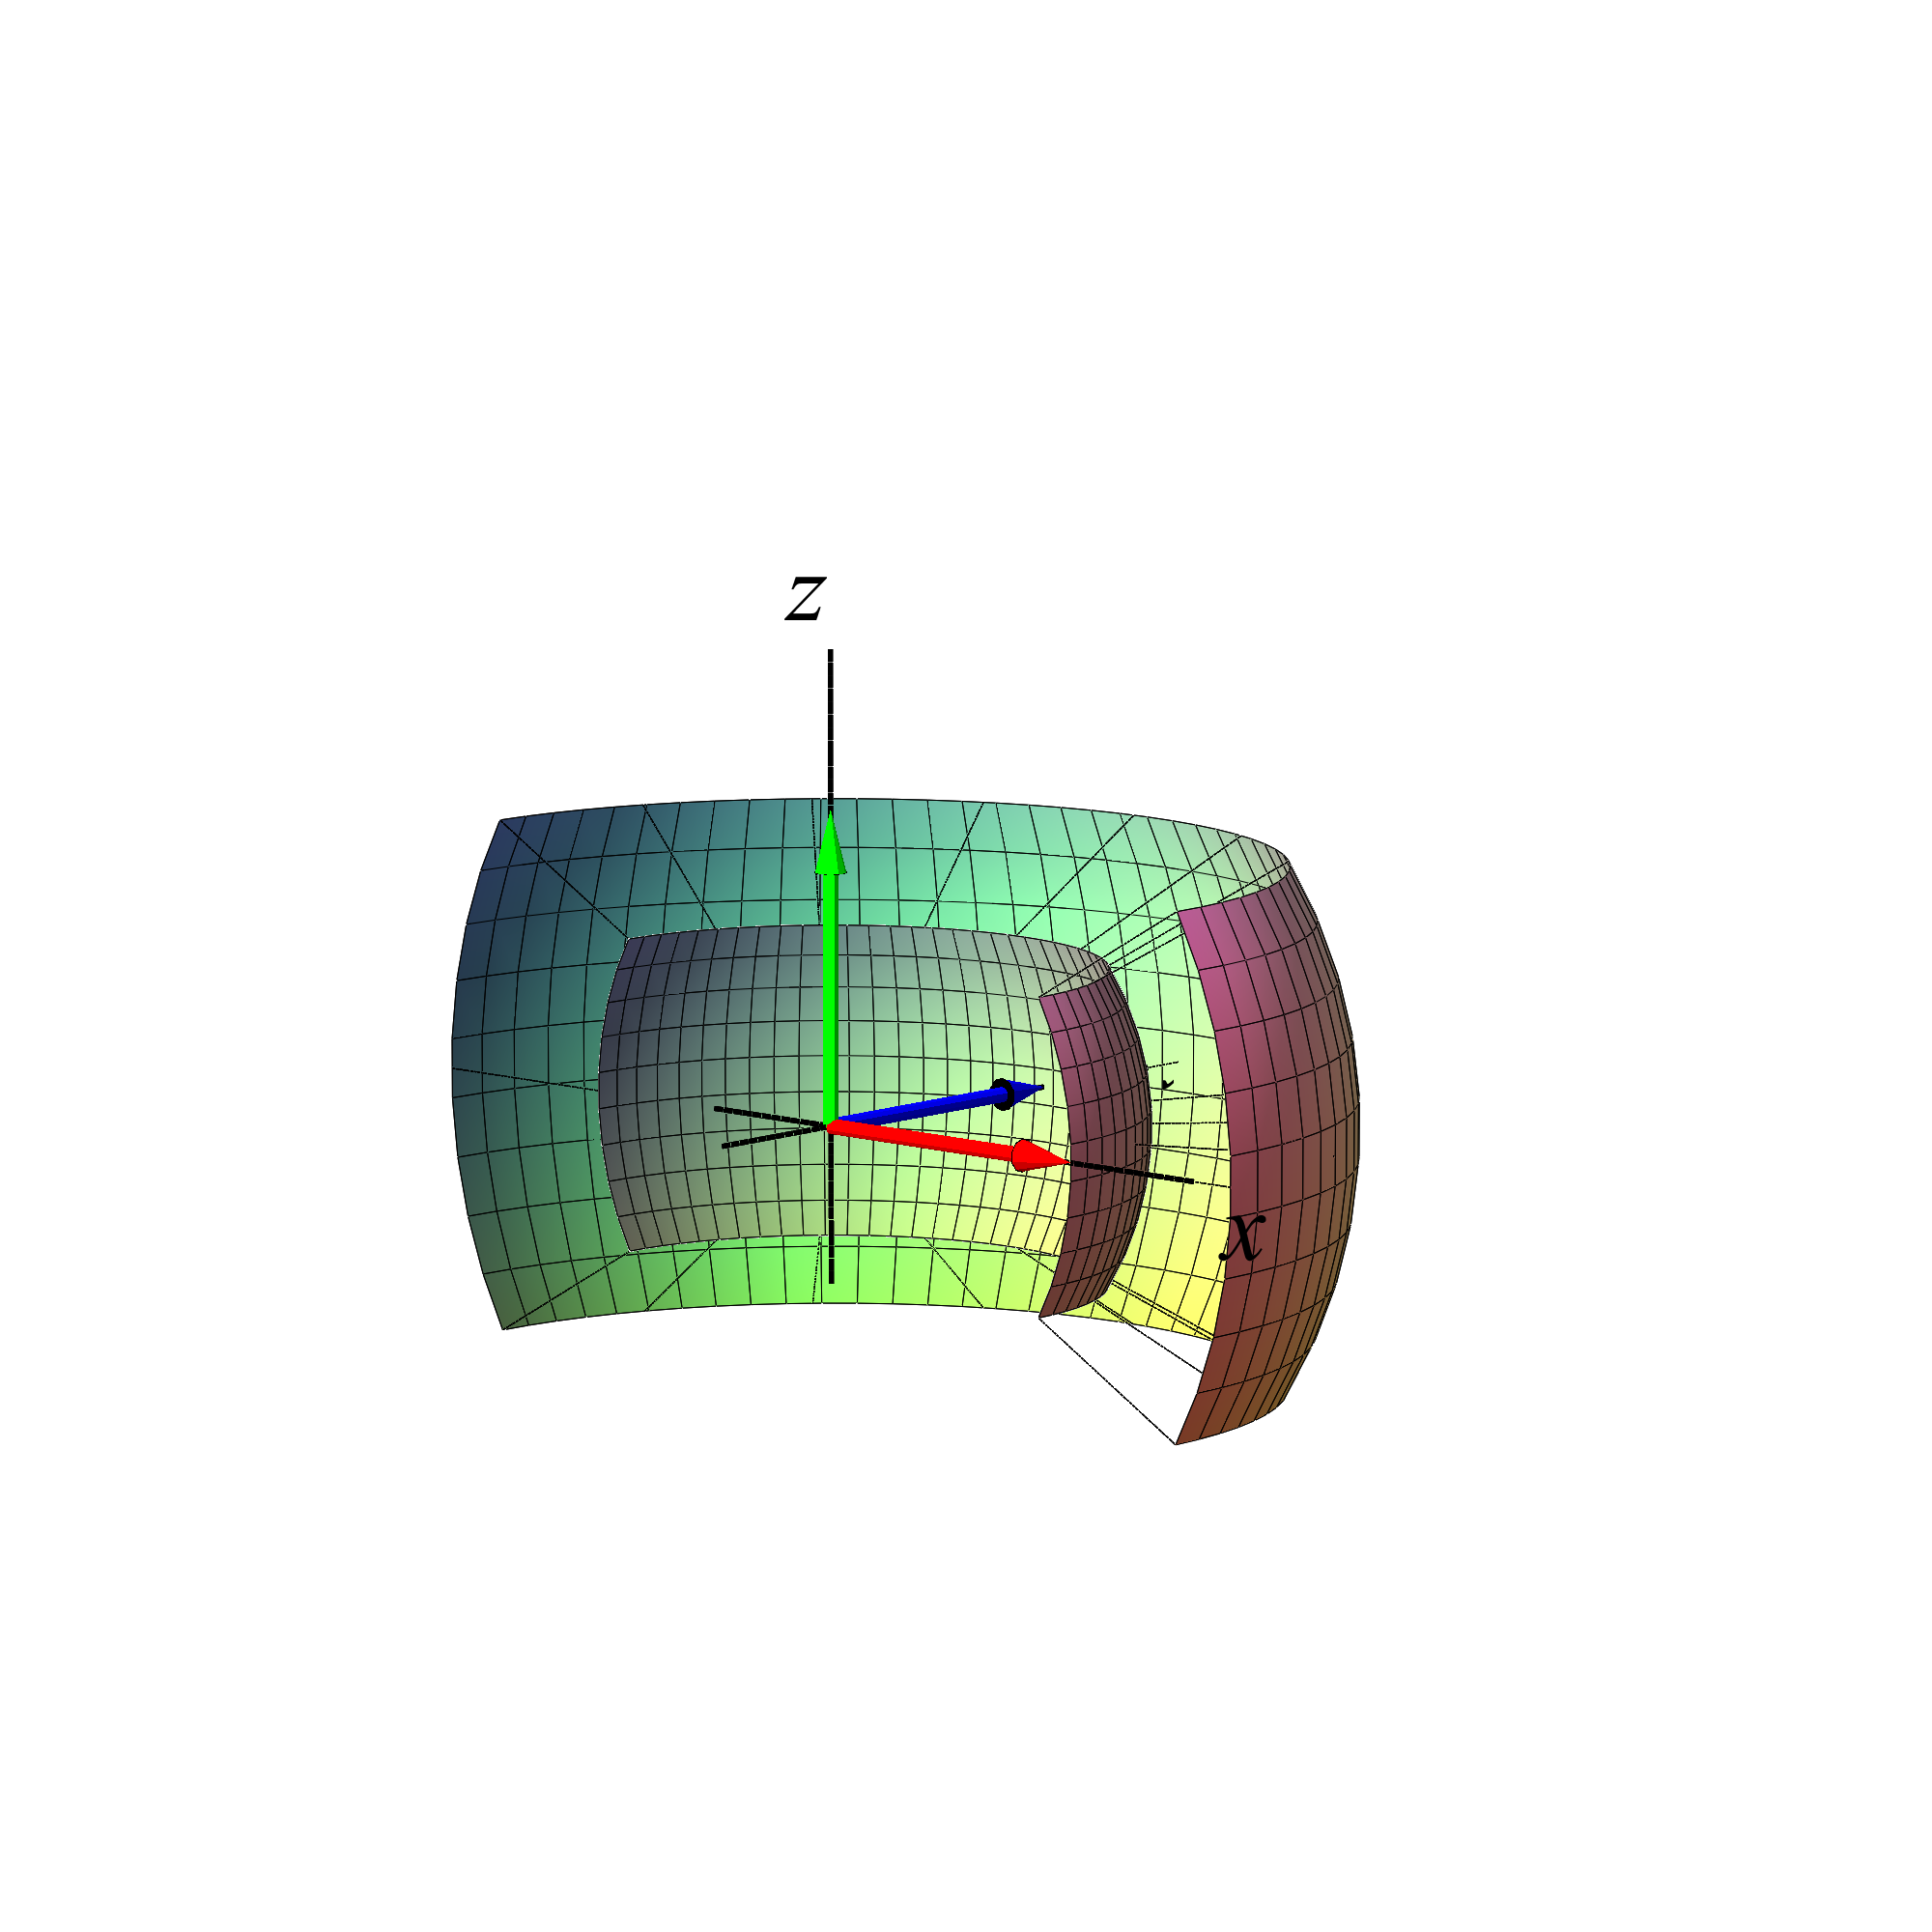
\includegraphics[height=70mm]{FIGS/plotNormalSphFlow} 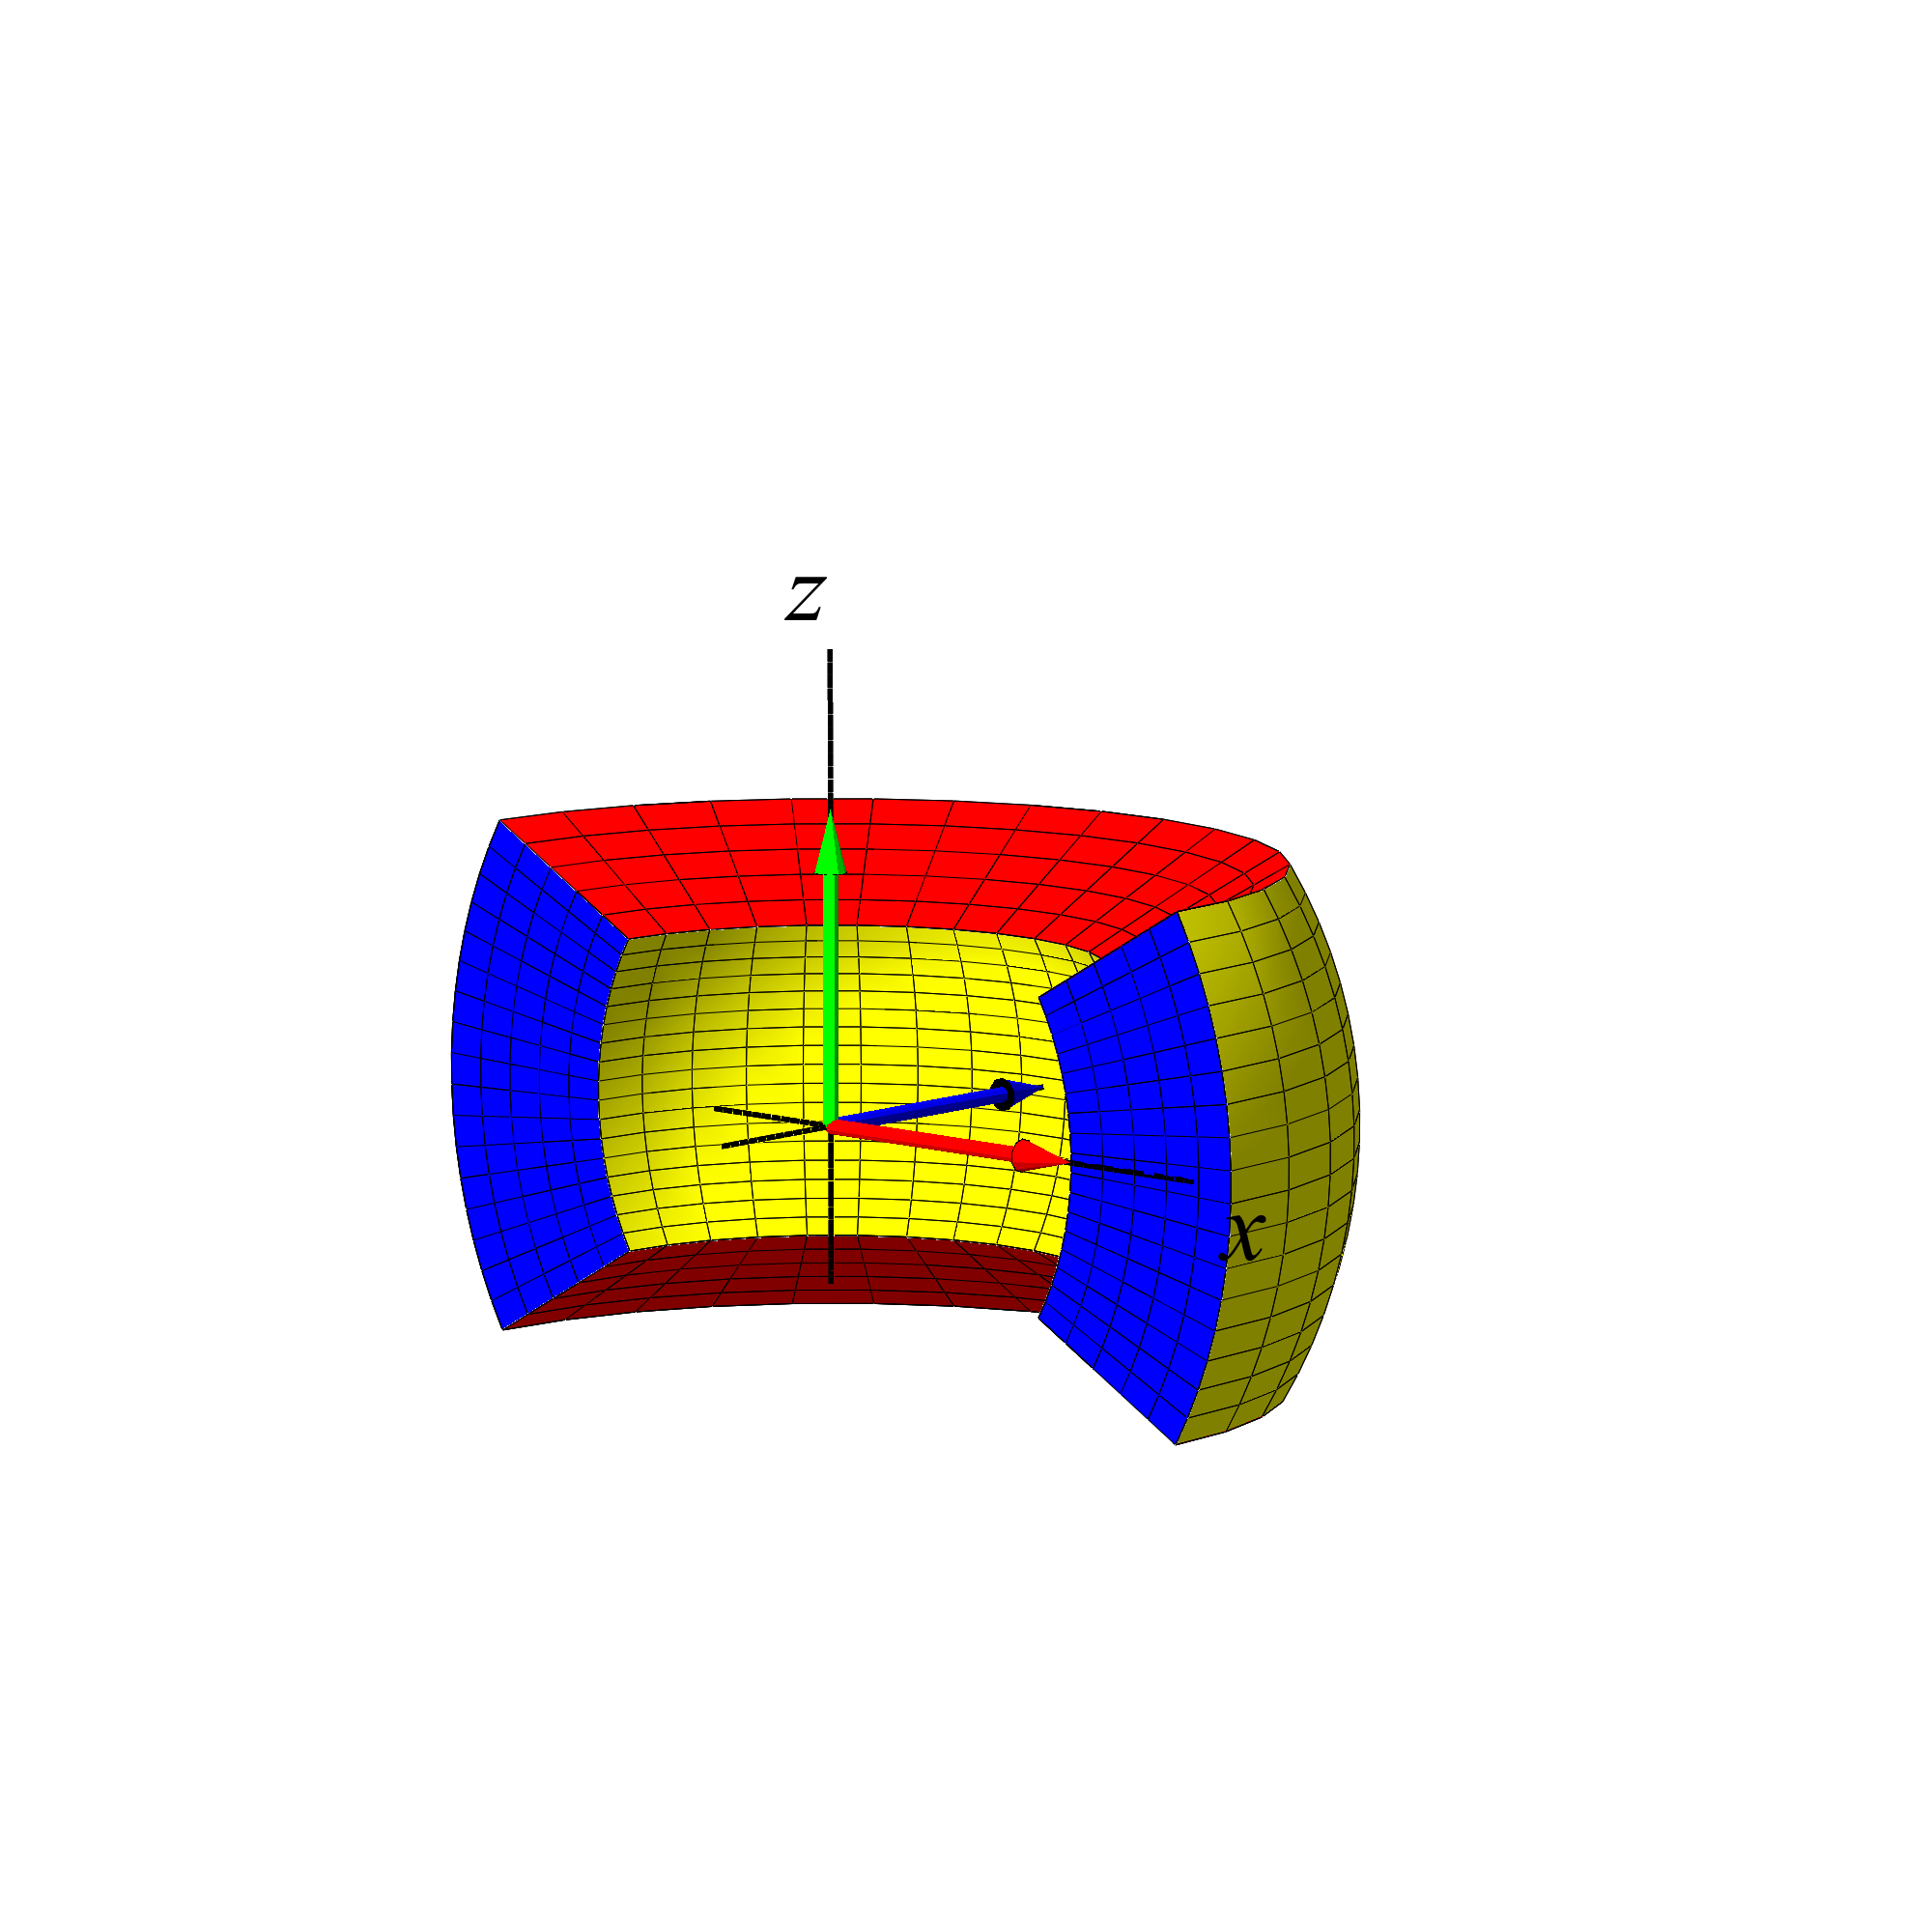
\includegraphics[height=70mm]{FIGS/plotNormalSphFlowSolid}}
\begin{center}
\caption{En tubulær skal der er defineret ved flow langs  \emph{enheds-normalvektorfeltet} $\mathbf{n}_{F}$
fra et
fladestykke af en kugleflade.} \label{figShell12B}
\end{center}
\end{figure}



%%%%%%%%%%%%%%%%%%%%%%%%%%%%%%%%%%%%%%%%%%%%%%%%%%%%%%%%%%%%%


Jacobi-funktionen for  ${\bf{R}}$ er
\begin{equation} \label{eqFatJac}
\begin{aligned}
\Jac_{{\bf{R}}}(u,v,w) \, &= \, |\left(
{\bf{R}}'_{u} \times {\bf{R}}'_{v}\right)\bm{\cdot}
{\bf{R}}'_{w}| \\ &= \, |\left( ({\bf{r}}'_{u} +
w\,{\bf{n}}'_{u} ) \times ({\bf{r}}'_{v}+ w\,
{\bf{n}}'_{v})\right)\bm{\cdot} {\bf{n}}_{F}| \quad .
\end{aligned}
\end{equation}
Da ${\bf{n}}_{F}$ er et enhedsvektorfelt som er
parallelt med ${\bf{r}}'_{u} \times
{\bf{r}}'_{v}$ langs $F_{\bf{r}}$, får vi
specielt (for $w\, = \, 0$):
\begin{equation} \label{eqFatJac0}
\begin{aligned}
\Jac_{{\bf{R}}}(u,v,0) \, &= \,
|\left({\bf{r}}'_{u} \times
{\bf{r}}'_{v}\right)\bm{\cdot} {\bf{n}}_{F}|
\\ &=  \, \Vert {\bf{r}}'_{u} \times
{\bf{r}}'_{v} \Vert   \\ &= \Jac_{{\bf{r}}}(u,v)
\, > \, 0 \quad .
\end{aligned}
\end{equation}


Afbildningen  ${\bf{R}}$ er regulær og bijektiv
på $D \times [0, t]$ - hvis blot $t$ er
tilstrækkelig lille. Det følger dels af
$\Jac_{{\bf{R}}}(u,v,0) \,
> \, 0$ og dels af kontinuiteten af
$\Jac_{{\bf{R}}}(u,v,w)$.\\

Værdien af $w$ betragtet som en funktion på
$\Omega_{t} \subset \mathbb{R}^{3}$ er en
differentiabel funktion af de tre rum-variable
$(x,y,z)$. Selv om dette kan forekomme at være
helt tydeligt, rent intuitivt, så er det faktisk
et resultat, der finder sin bedste formulering og
begrundelse i den såkaldte {\em{{invers
funktions-sætning}}}, som dyrkes i kurset
\href{http://www.mat.dtu.dk/Uddannelse/Civil.aspx?coursecode=01330}{Matematik 3}:

%%%%%%%%%%%%%%%%%%%%%%%%%%%%%%%%%%%%%%%%%%%%%%%%%%%%%%%%%%%%%%%%%%%%%

\begin{theorem} [Invers funktionssætning] \label{thmInvFunct}
Lad $Q$ betegne en åben mængde i $\mathbb{R}^{3}$
og lad $\,{\bf{f}}\, : Q \to \mathbb{R}^{3}$
betegne en differentiabel bijektiv afbildning med
$\Jac_{\bf{f}}({\bf{x}}) \,
> \, 0\,$ for alle ${\bf{x}} \in Q$. \\

 Så er den omvendte afbildning ${\bf{f}}^{\circ -1}\, :
{\bf{f}}(Q) \to Q$ også differentiabel med
$\Jac_{\bf{f}^{\circ -1}}({\bf{y}}) \,
> \, 0\,$ for alle ${\bf{y}} \in {\bf{f}}(Q)$.
\end{theorem}


Intuitionen er altså i dette tilfælde præcis og korrekt. Når
$t$ er tilstrækkelig lille, så er $w$ en
differentiabel funktion af de tre rum-variable,
$(x,y,z)$; lad os kalde den funktion $h(x,y,z)$,
$(x,y,z) \in \Omega_{t}$. Den funktion har så en
egentlig gradient $\bm{\nabla}(h)(x,y,z)$, som er
vinkelret på niveaufladerne for $h$. Specielt er
$\bm{\nabla}(h)$ vinkelret på top-fladen
$F_{t}\,=\,F_{\bf{R}}(t)$ af skallen
$\Omega_{t}$, hvor $h\, = \, t$ og den er
tilsvarende vinkelret på basis-fladen
$F_{0}\,=\,F_{\bf{R}}(0)\,
= \, F_{\bf{r}}$, hvor $h\, = \, 0$. \\

Gradienten  $\bm{\nabla}(h)$ er faktisk præcis lig med
${\bf{n}}_{F}$ på basis-fladen. For at indse
dette behøver vi kun at vise, at længden af
gradienten der er 1. Retningen er jo den samme.
Lad derfor $(u_{0},v_{0})$ betegne et punkt i $D$
og betragt restriktionen af $h$ til den rette
linje ${\bf{r}}(u_{0},v_{0}) +
w\,{\bf{n}}(u_{0},v_{0})$, hvor $w \in [0, t]$.
Lad os benytte notationen ${\bf{r}}_{0}\, = \,
{\bf{r}}(u_{0},v_{0})$ og ${\bf{n}}_{0}\, = \,
{\bf{n}}(u_{0},v_{0})$. Så giver kædereglen
\begin{equation}
\begin{aligned}
1 \, &= \, |\,\frac{d}{dw}h({\bf{r}}_{0} +
w\,{\bf{n}}_{0})\,| \,
\\ &= \, |\,{\bf{n}}_{0} \bm{\cdot} \bm{\nabla}(h)({\bf{r}}_{0} +
w\,{\bf{n}}_{0})\,| \\ &= \Vert
\bm{\nabla}(h)({\bf{r}}_{0} + w\,{\bf{n}}_{0})\,\Vert
\quad ,
\end{aligned}
\end{equation}
således at vi på fladen $F_{\bf{r}}$, hvor $w =
0$, har $\,\Vert \bm{\nabla}(h)({\bf{r}}_{0}) \Vert \,
= \, 1\,$. Det var det, vi skulle vise. Vi har derfor:
\begin{equation}
\bm{\nabla}(h)_{|_{F}} \, = \,{\bf{n}}_{F} \quad .
\end{equation}

\begin{think}
Funktionen $h(x,y,z)$ er den {\em{Euklidiske
afstand}} fra punktet $(x,y,z)$
til fladen $F_{\bf{r}}$. Lokalt, dvs. tilstrækkeligt tæt på (og i normalretningen af) fladen $F_{\bf{r}}$ er
$\bm{\nabla}h(x,y,z)$ en \emph{udvidelse} af enhedsnormalvektorfeltet $\mathbf{n}_{F}$ til fladen.
Vektorfeltet $\bm{\nabla}h(x,y,z)$ er selv et enhedsvektorfelt.
Ved at lade $F_{\bf{r}}$ flyde tiden $t$ langs flowkurverne for $\bm{\nabla}h(x,y,z)$ dannes (udfejes) det rumlige område, den massive skal, $\Omega_{t}$, se figurerne \ref{figShell12A}, \ref{figShell12B}.
\end{think}



%%%%%%%%%%%%%%%%%%%%%%%%%%%%%%%%%%%%%%%%%%%%%%%%%%%%%%%%%%%%%%%%%%%%%%%%%%
\subsection{Integration i skallen} \label{secShellInt}
For en funktion $f(x,y,z)$ som er defineret i
$\Omega_{t}$ fås integralet af $f$ over området
således:
\begin{equation}
\begin{aligned}
&\phantom{= \,\,\,}\int_{\Omega_{t}}\, f\,d\mu \,
\\ &= \,\int_{0}^{t}\left(\int_{D}\,
f({\bf{R}}(u,v,w))
\Jac_{{\bf{R}}}(u,v,w)\,du\,dv\,\right)dw  \quad
.
\end{aligned}
\end{equation}
Den $t$-afledede af dette integral er, for $t =
0$, simpelthen fladeintegralet af $f$ over $F_{\bf{r}}$:
\begin{lemma}[Fladeintegral som $t$-afledet af rumintegral] \label{lemFladeIntFraRumint}
\begin{equation} \label{eqShellDeriv}
\left(\frac{d}{dt}\right)_{|_{t=0}}\int_{\Omega_{t}}\,
f\,d\mu \, \, = \,
 \int_{F_{\bf{r}}}\,f \, d\mu \quad .
\end{equation}
\end{lemma}
\begin{bevis}
Det følger direkte af fundamentalsætningen
\ref{thmFundamCalc}:
\begin{equation}
\begin{aligned}
&\phantom{= \,\,\,}\left(\frac{d}{dt}\right)_{|_{t=0}}\int_{\Omega_{t}}\, f\,d\mu \, \\
&= \,
\left(\frac{d}{dt}\right)_{|_{t=0}}\int_{0}^{t}\left(\int_{D}\,
f({\bf{R}}(u,v,w))
\Jac_{{\bf{R}}}(u,v,w)\,du\,dv\,\right)dw \\ &=
\, \int_{D}\, f({\bf{R}}(u,v,0)) \Jac_{{\bf{R}}}(u,v,0)\,du\,dv \\
&= \, \int_{D} \,f({\bf{r}}(u,v))
\Jac_{{\bf{r}}}(u,v)\,du\,dv \\ &= \,
 \int_{F_{\bf{r}}}\,f \, d\mu \quad .
\end{aligned}
\end{equation}

\end{bevis}


%%%%%%%%%%%%%%%%%%%%%%%%%%%%%%%%%%%%%%%%%%%%%%%%%%%%%%%%%%%%%%%%%%%%%%%%%%
%%%%%%%%%%%%%%%%%%%%%%%%%%%%%%%%%%%%%%%%%%%%%%%%%%%%%%%%%%%%%%%%%%%%%%%%%%
%%%%%%%%%%%%%%%%%%%%%%%%%%%%%%%%%%%%%%%%%%%%%%%%%%%%%%%%%%%%%%%%%%%%%%%%%%


%%%%%%%%%%%%%%%%%%%%%%%%%%%%%%%%%%%%%%%%%%%%%%%%%%%%%%%%%%%%%%%%%%%%%%%%%%
\subsection{The Wall - Væggen} \label{secWall}

Skallen $\Omega_{t}$ har en rand $\partial
\Omega_{t}$ som består af top-fladen $F_{t}$,
basis-fladen $F_{0} \,=\, F_{\bf{r}} \, = \,
F_{\bf{R}}(0)$ og en 'væg'  $W_{t}$ med højden
$t$. Se figurerne \ref{figShell12A} og \ref{figShell12B}. Væg-komponenten
fås ved restriktion af afbildningen ${\bf{R}}$
til $\partial D \times [0, t]$ således:
\begin{equation}
\begin{aligned}
W_{t}: \qquad  {\bf{B}}(\theta, w) \, &=
{\bf{R}}(u(\theta), v(\theta), w) \\ &=
{\bf{r}}(u(\theta), v(\theta)) +
w\,{\bf{n}}(u(\theta), v(\theta)) \\ &=
{\bf{b}}(\theta) + w\,{\bf{n}}({\bf{d}}(\theta))
\,\, , \,\, \theta \in I \,\, , \, \, w \in [0,
t] \quad .
\end{aligned}
\end{equation}


Jacobi-funktionen for denne afbildning er derfor
\begin{equation} \label{eqFatWall}
\begin{aligned}
\Jac_{{\bf{B}}}(\theta, w) \, &= \, \Vert {\bf{B}}'_{\theta} \times {\bf{B}}'_{w} \Vert \\
&= \, \Vert ({\bf{b}}'_{\theta} + w\,({\bf{n}}
\circ {\bf{d}})'_{\theta} ) \times {\bf{n}}_{F}
\Vert \quad .
\end{aligned}
\end{equation}
Da ${\bf{n}}_{F}$ står vinkelret på  fladen
$F_{\bf{r}}$ og derfor også på randen $\partial
F_{\bf{r}}$ (parametriseret via ${\bf{b}}$), får
vi:
\begin{equation}
\begin{aligned}
\Jac_{{\bf{B}}}(\theta, 0) = \,
\Vert{\bf{b}}'_{\theta} \times {\bf{n}}_{F} \Vert
\, &= \,\Vert {\bf{b}}'_{\theta} \Vert \, = \,
\Jac_{{\bf{b}}}(\theta)\, \quad .
\end{aligned}
\end{equation}


%%%%%%%%%%%%%%%%%%%%%%%%%%%%%%%%%%%%%%%%%%%%%%%%%%%%%%%%%%%%%%%%%%%%%%%%%%
\subsection{Integration langs væggen} \label{secWallInt}
For en given funktion $g(x,y,z)$ defineret på
$W_{t}$ fås integralet af $g$ over den flade:
\begin{equation}
\int_{W_{t}}\, g\, d\mu \, = \,
\int_{0}^{t}\left(\int_{I}\,g({\bf{B}}(\theta,
w))\,\Jac_{{\bf{B}}}(\theta, w)\,d\theta\right)
dw \quad.
\end{equation}

Den $t$-afledede af dette integral er, for $t=0$,
kurve-integralet af $g$ over $\partial F$:

\begin{lemma}[Kurveintegral som $t$-afledet af fladeintegral] \label{lemKurveFraFlade}
\begin{equation}\label{eqFatWallTderiv}
\left(\frac{d}{dt}\right)_{|_{t=0}}\int_{W_{t}}\,
g\,d\mu \, = \,
 \int_{\partial F}\,g \, d\mu \quad .
\end{equation}
\end{lemma}

\begin{bevis}
Det følger igen af fundamentalsætningen, Sætning
\ref{thmFundamCalc}:
\begin{equation}
\begin{aligned}
&\phantom{= \,\,\,}\left(\frac{d}{dt}\right)_{|_{t=0}}\int_{W_{t}}\, g\,d\mu\, \\
&= \,
\left(\frac{d}{dt}\right)_{|_{t=0}}\int_{0}^{t}\left(\int_{I}\, g({\bf{B}}(\theta,w)) \Jac_{{\bf{B}}}(\theta,w)\,d\theta\,\right)dw \\
&= \, \int_{I}\, g({\bf{B}}(\theta,0)) \Jac_{{\bf{B}}}(\theta,0)\,d\theta \\
&= \, \int_{I} \,g({\bf{b}}(\theta)) \Jac_{{\bf{b}}}(\theta)\,d\theta \\
&= \,
 \int_{\partial F}\,g \, d\mu \quad .
\end{aligned}
\end{equation}
\end{bevis}

%%%%%%%%%%%%%%%%%%%%%%%%%%%%%%%%%%%%%%%%%%%%%%%%%%%%%%%%%%%%%%%%%%%%%%%%%%
\subsection{Bevis for Stokes' sætning} \label{secStokesSurf}

Vi er nu parate til at bevise Sætning
\ref{thmStokes}.
\begin{bevis}
Funktionen  $h(x,y,z)$ fra det foregående afsnit
\ref{secShell} indsættes i stedet for
$\psi(x,y,z)$ i Sætning \ref{thmGaussStokes},
ligning (\ref{eqIntDivRotB}). Med
integrations-området $\Omega \, = \, \Omega_{t}$
får vi så:
\begin{equation} \label{eqReduce}
\begin{aligned}
\int_{\Omega_{t}}\,
\Rot({\bf{V}})&\bm{\cdot}\bm{\nabla}(h)\, d\mu \,\\ &= \,
\int_{\partial \Omega_{t}}\,
\left({\bf{n}}_{\partial \Omega_{t}}\, \times
{\bf{V}}\right) \bm{\cdot} \bm{\nabla}(h)
 \, \,d\mu  \\ &= \,
\int_{F_{t}}\,  \left({\bf{n}}_{F_{t}}\, \times
{\bf{V}}\right) \bm{\cdot} \bm{\nabla}(h)
 \, \,d\mu \, \\ &  - \,
 \int_{F_{0}}\,  \left({\bf{n}}_{F_{0}}\,
\times {\bf{V}}\right) \bm{\cdot} \bm{\nabla}(h)
 \, \,d\mu \, \\ &  + \,
 \int_{W_{t}}\,  \left({\bf{n}}_{W_{t}}\,
\times {\bf{V}}\right) \bm{\cdot} \bm{\nabla}(h)
 \, \,d\mu
\quad .
\end{aligned}
\end{equation}
Men i ligning (\ref{eqReduce}) har vi
\begin{equation}
\begin{aligned}
\int_{F_{t}}\,  \left({\bf{n}}_{F_{t}}\, \times
{\bf{V}}\right) \bm{\cdot} \bm{\nabla}(h)
 \, \,d\mu\,  &= \, 0 \quad \textrm{og} \\
 \int_{F_{0}}\,  \left({\bf{n}}_{F_{0}}\,
\times {\bf{V}}\right) \bm{\cdot} \bm{\nabla}(h)
 \, \,d\mu \, &= \, 0 \quad,
\end{aligned}
\end{equation}
idet $\bm{\nabla}(h)$ er vinkelret på  begge fladerne
$F_{t}$ og $F_{0}$ således at  $\bm{\nabla}(h)$ er
proportional med henholdsvis ${\bf{n}}_{F_{t}}$
og
${\bf{n}}_{F_{0}}$ på de respektive flader.\\





Langs $\partial F \subset W_{t}$ har vi
${\bf{n}}_{W_{t}}\, = \, {\bf{e}}_{\partial F}
\times {\bf{n}}_{F}$ og derfor
${\bf{e}}_{\partial F}\, = \, {\bf{n}}_{F}\,
\times {\bf{n}}_{W_{t}}$ - i overensstemmelse med
orienterings-reglen i Sætning \ref{thmStokes}.
Hvis vi $t$-afleder begge sider af den reducerede
ligning  (\ref{eqReduce}) får vi:
\begin{equation}
\begin{aligned}
&\phantom{=
\,\,\,}\left(\frac{d}{dt}\right)_{|_{t=0}}\int_{\Omega_{t}}\,
\Rot({\bf{V}})\bm{\cdot}\bm{\nabla}(h)\, d\mu \, \\ &= \,
\left(\frac{d}{dt}\right)_{|_{t=0}}\int_{W_{t}}\,
\left({\bf{n}}_{W_{t}}\, \times {\bf{V}}\right)
\bm{\cdot} \bm{\nabla}(h)
 \, \,d\mu
\quad ,
\end{aligned}
\end{equation}
således at vi endelig har - i kraft af
ligningerne (\ref{eqShellDeriv}) og
(\ref{eqFatWallTderiv}):
\begin{equation}
\begin{aligned}
&\phantom{= \,\,\,}\int_{F}\, \Rot({\bf{V}})\bm{\cdot}
{\bf{n}}_{F} \, d\mu \,
\\ &= \,\int_{\partial F}\,
\left({\bf{n}}_{W_{t}}\, \times {\bf{V}}\right)
\bm{\cdot} {\bf{n}}_{F}
 \, \,d\mu \\ &= \,
\int_{\partial F}\,
{\bf{V}}\bm{\cdot}\left({\bf{n}}_{F}\, \times
{\bf{n}}_{W_{t}} \right)
 \, \,d\mu \\ &= \,
\int_{\partial F}\, {\bf{V}} \bm{\cdot}
{\bf{e}}_{\partial F}
 \, \,d\mu
\quad .
\end{aligned}
\end{equation}
Stokes' sætning er dermed bevist.
\end{bevis}


%%%%%%%%%%%%%%%%%%%%%%%%%%%%%%%%%%%%%%%%%%%%%%%%%%%%%%%%%%%%%%%%%%%%%%%%%%%%
%%%%%%%%%%%%%%%%%%%%%%%%%%%%%%%%%%%%%%%%%%%%%%%%%%%%%%%%%%%%%%%%%%%%%%%%%%%%
%%%%%%%%%%%%%%%%%%%%%%%%%%%%%%%%%%%%%%%%%%%%%%%%%%%%%%%%%%%%%%%%%%%%%%%%%%%%
%%%%%%%%%%%%%%%%%%%%%%%%%%%%%%%%%%%%%%%%%%%%%%%%%%%%%%%%%%%%%%%%%%%%%%%%%%%%

\section{Verificering af Stokes' sætning i konkrete eksempler} \label{secVerif}


I lighed med Gauss' divergens-sætning kan Stokes'
sætning verificeres ved i konkrete givne tilfælde
at beregne \emph{begge sider} af identiteten
(\ref{eqStokes}) i Stokes' sætning.



%%%%%%%%%%%%%%%%%%%%%%%%%%%%%%%%%%%%%%%%%%%%%%%%%%%%%%%%%%%%%%%%%%%%%%%%%%%%
%%%%%%%%%%%%%%%%%%%%%%%%%%%%%%%%%%%%%%%%%%%%%%%%%%%%%%%%%%%%%%%%%%%%%%%%%%%%
%%%%%%%%%%%%%%%%%%%%%%%%%%%%%%%%%%%%%%%%%%%%%%%%%%%%%%%%%%%%%%%%%%%%%%%%%%%%
%%%%%%%%%%%%%%%%%%%%%%%%%%%%%%%%%%%%%%%%%%%%%%%%%%%%%%%%%%%%%%%%%%%%%%%%%%%%




\begin{example}[Stokes' sætning med en cirkelskive] \label{exampDiskStokes}
En standard cirkelskive i $(x,y)$-planen er givet ved sin sædvanlige parameterfremstilling:
\begin{equation}
F_{\mathbf{r}}\quad : \quad \mathbf{r}(u,v) = (u\cdot \cos(v), u \cdot \sin(v), 0) \quad , \quad (u,v) \in [0, 1] \times [-\pi, \pi]
\end{equation}
med Jacobifunktionen
\begin{equation}
\Jac_{\mathbf{r}}(u,v) = u \quad ,
\end{equation}
standard enhedsnormalvektorfelt til fladen
\begin{equation}
\mathbf{n}_{F} = (0,0,1) \quad ,
\end{equation}
og standard enheds-tangentvektorfelt langs den \emph{cirkulære} rand $\partial F$:
\begin{equation}
\mathbf{e}_{\partial F} = \mathbf{r}'_{v}(1, v) = (-\sin(v)\, , \, \cos(v)\, , \, 0 ) \quad .
\end{equation}
\begin{aha}
Bemærk, at det er $\mathbf{r}(1, v)$, $v \in [-\pi, \pi]$,  der giver \emph{hele randen}, at $\mathbf{r}'_{v}(1, v)$ er en enhedsvektor for alle $v$, og at $\mathbf{r}'_{v}(1, v)\times \mathbf{n}_{F}$ peger væk fra cirkelskiven langs hele randkurven.\\
\end{aha}
Et glat vektorfelt i rummet er givet ved sine koordinatfunktioner således:
\begin{equation}
\mathbf{V}(x,y,z) = (x\cdot y \, , \, x \, , \, x^{2}) \quad ,
\end{equation}
og har det tilhørende rotationsvektorfelt
\begin{equation}
\Rot(\mathbf{V})(x,y,z) = (0\, , \, -2\cdot x \, , \,  1-x) \quad .
\end{equation}
Vi vil verificere Stokes' sætning ved at beregne ''begge sider'' af ligning (\ref{eqStokes}) i dette konkrete tilfælde.\\

Den totale flux af vektorfeltet $\Rot(\mathbf{V})(x,y,z)$ igennem $F_{\mathbf{r}}$ i retning af standard-enhedsnormalen $\mathbf{n}_{F} = (0,0,1)$ er
\begin{equation}
\begin{aligned}
\Flux(\Rot(\mathbf{V}), F_{\mathbf{r}} ) &= \int_{F_{\mathbf{r}}}\Rot(\mathbf{V}) \bm{\cdot} \mathbf{n}_{F} \, d\mu \\
&= \int_{F_{\mathbf{r}}} (1- x) \, d\mu \\
&= \int_{-\pi}^{\pi}\int_{0}^{1}(1 - u\cdot \cos(v)) \cdot u \, du \, dv \\
&= \int_{-\pi}^{\pi}\left(\frac{1}{2} - \frac{1}{3}\cdot \cos(v)\right)\, dv \\
&= \pi \quad .
\end{aligned}
\end{equation}
Cirkulationen af vektorfeltet $\mathbf{V}(x,y,z)$ langs $\partial F_{\mathbf{r}}$ i retning af stan\-dard-en\-heds\-tan\-gent\-vek\-to\-rfeltet $\mathbf{e}_{\partial F} = (-\sin(v), \, \cos(v)\, , \, 0 )$ er
\begin{equation}
\begin{aligned}
\operatorname{Cirk}(\mathbf{V}, \partial F) &= \int_{\partial F}\mathbf{V} \bm{\cdot} \mathbf{e}_{\partial F} \, d\mu \\
&= \int_{-\pi}^{\pi}\mathbf{V}(\mathbf{r}(1, v)) \bm{\cdot}  (-\sin(v),  \, \cos(v)\, , \, 0 ) \, dv \\
&= \int_{-\pi}^{\pi} (\cos(v)\cdot \sin(v)\, , \, \cos(v) \, , \, * ) \bm{\cdot}  (-\sin(v), \, \cos(v)\, , \, 0 ) \, dv \\
&= \int_{-\pi}^{\pi} (- \cos(v)\cdot \sin^{2}(v) + \cos^{2}(v))  \, dv \\
&= \int_{-\pi}^{\pi} \cos^{2}(v)  \, dv \\
&= \frac{1}{2}\int_{-\pi}^{\pi} \left( \cos^{2}(v) + \sin^{2}(v)\right) \, dv \\
&= \frac{1}{2}\int_{-\pi}^{\pi} 1 \, dv \\
&= \pi \quad .
\end{aligned}
\end{equation}
Begge sider i ligningen (\ref{eqStokes}) giver altså $\pi$ i dette eksempel -- og vi har derfor verificeret Stokes' sætning.
\end{example}



\begin{figure}[h]
\centerline{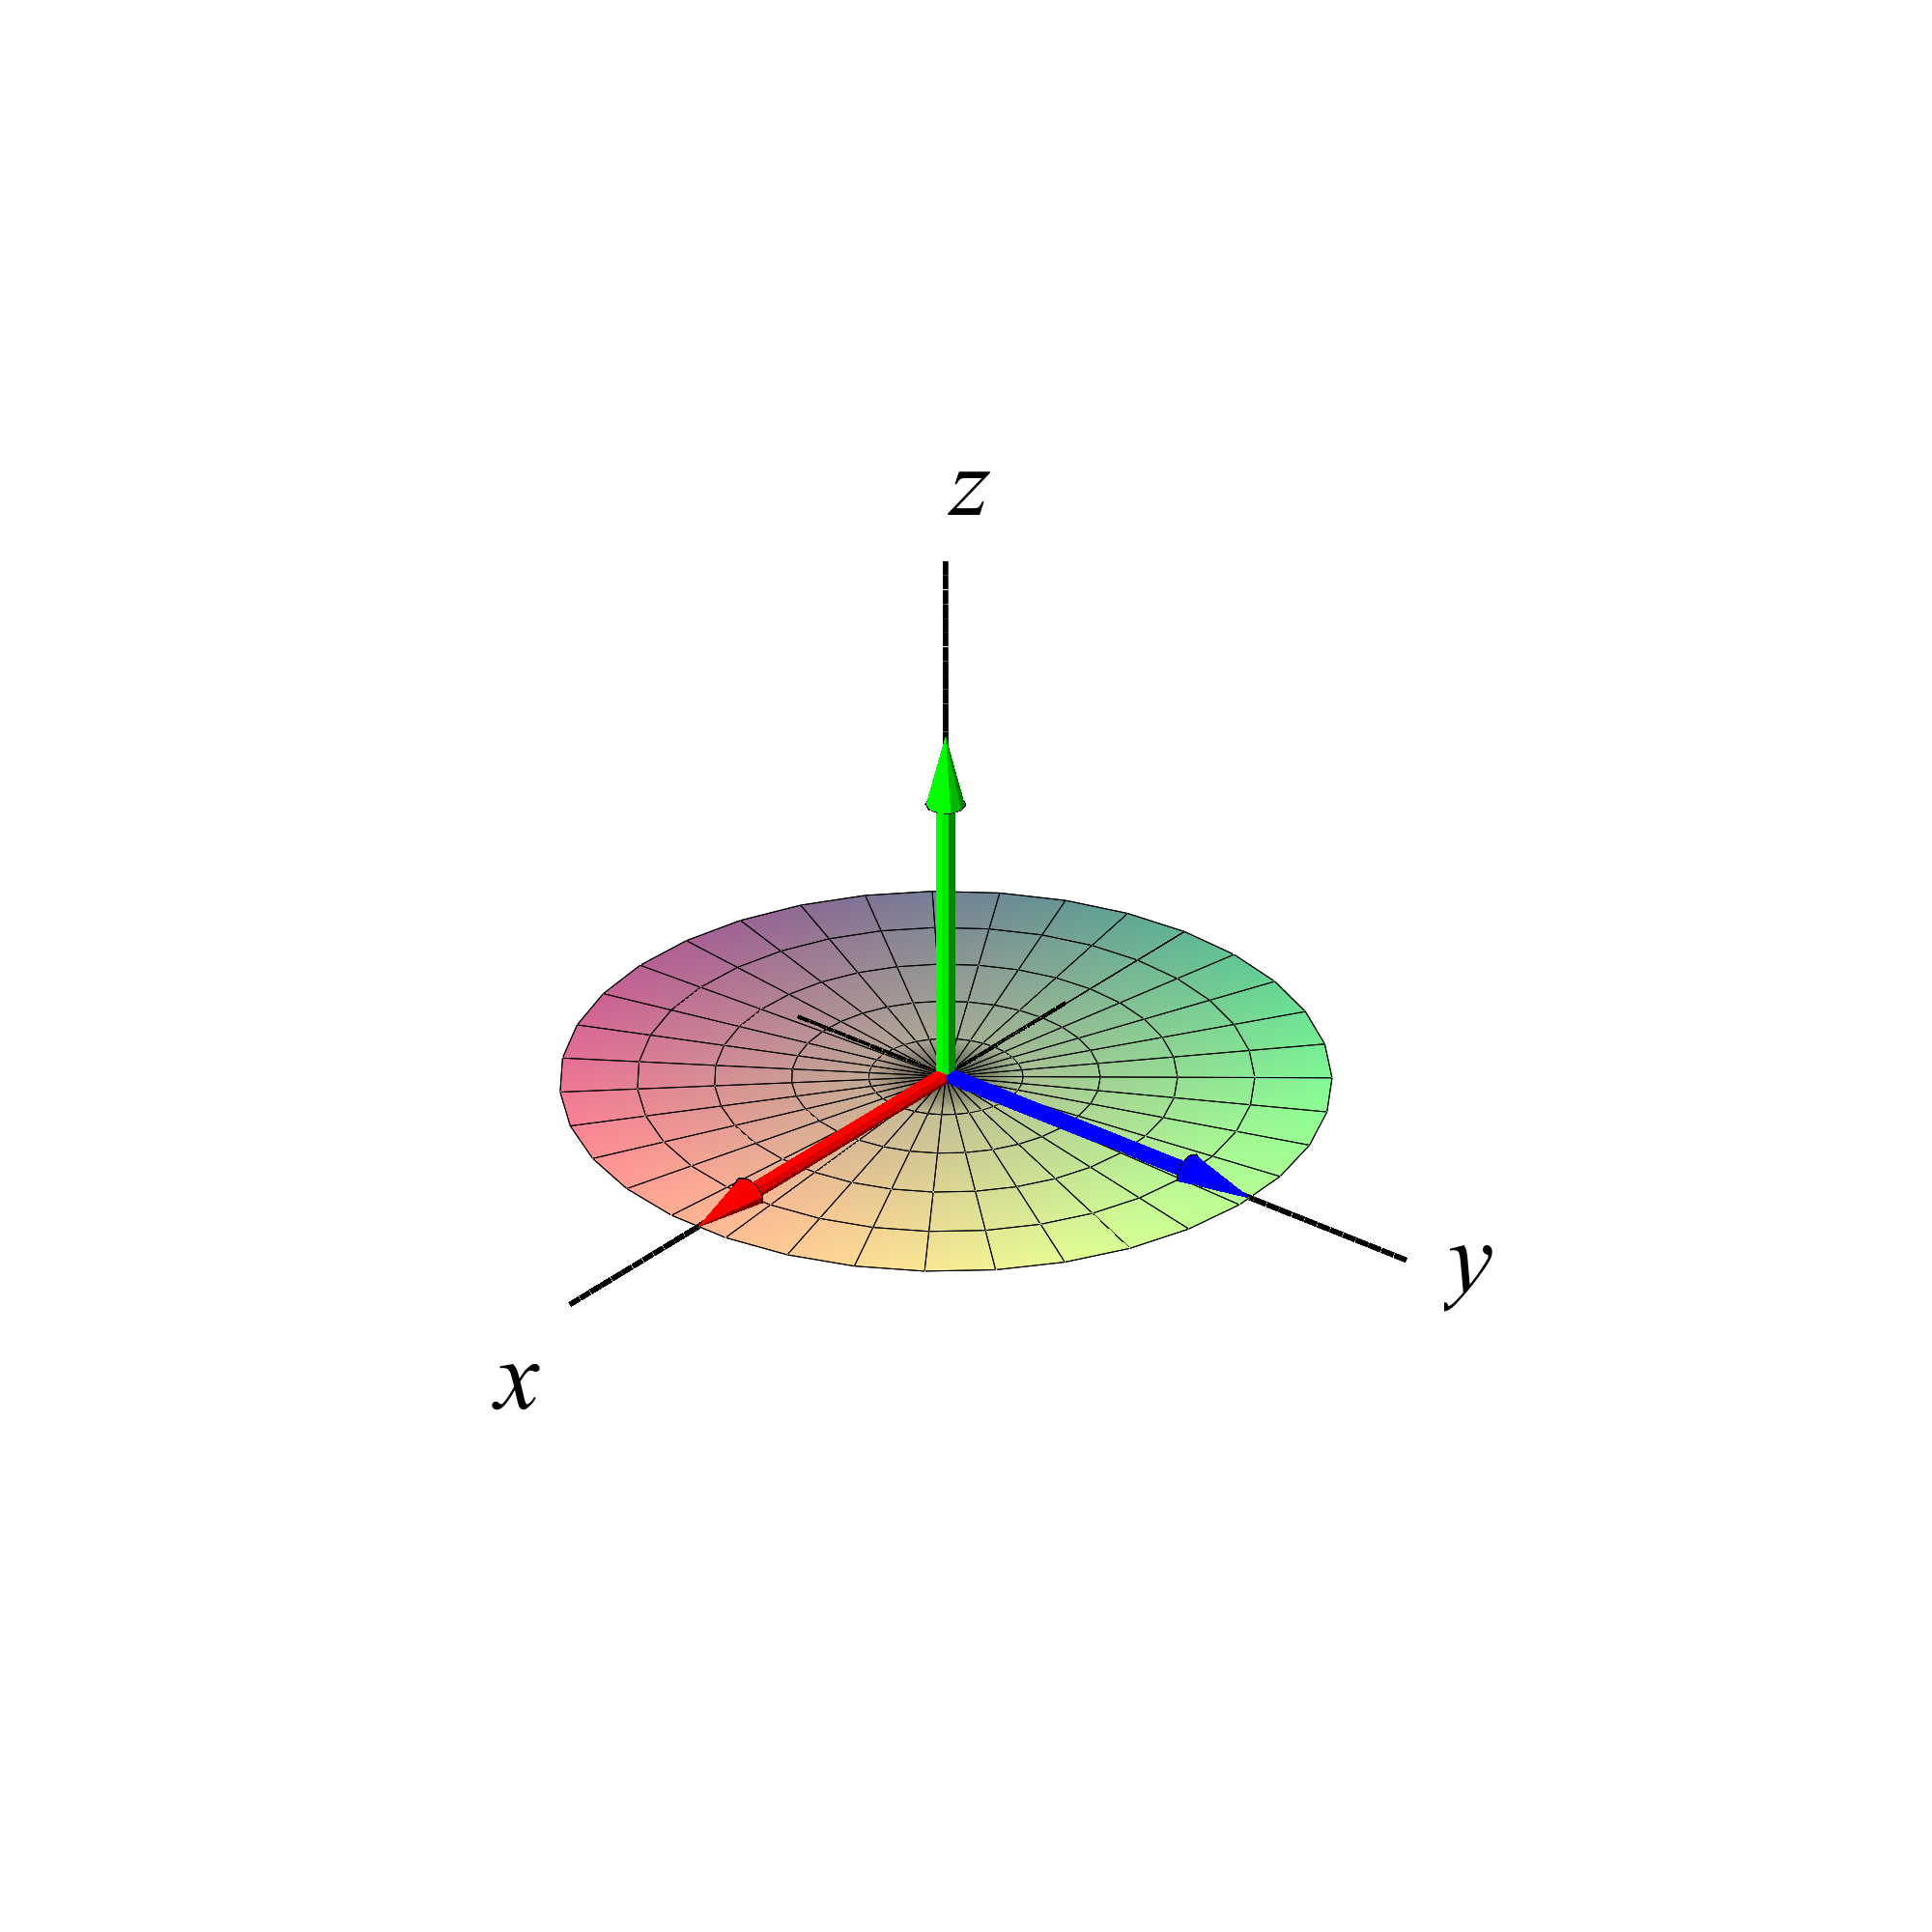
\includegraphics[height=70mm]{FIGS/plotDiskStokes1}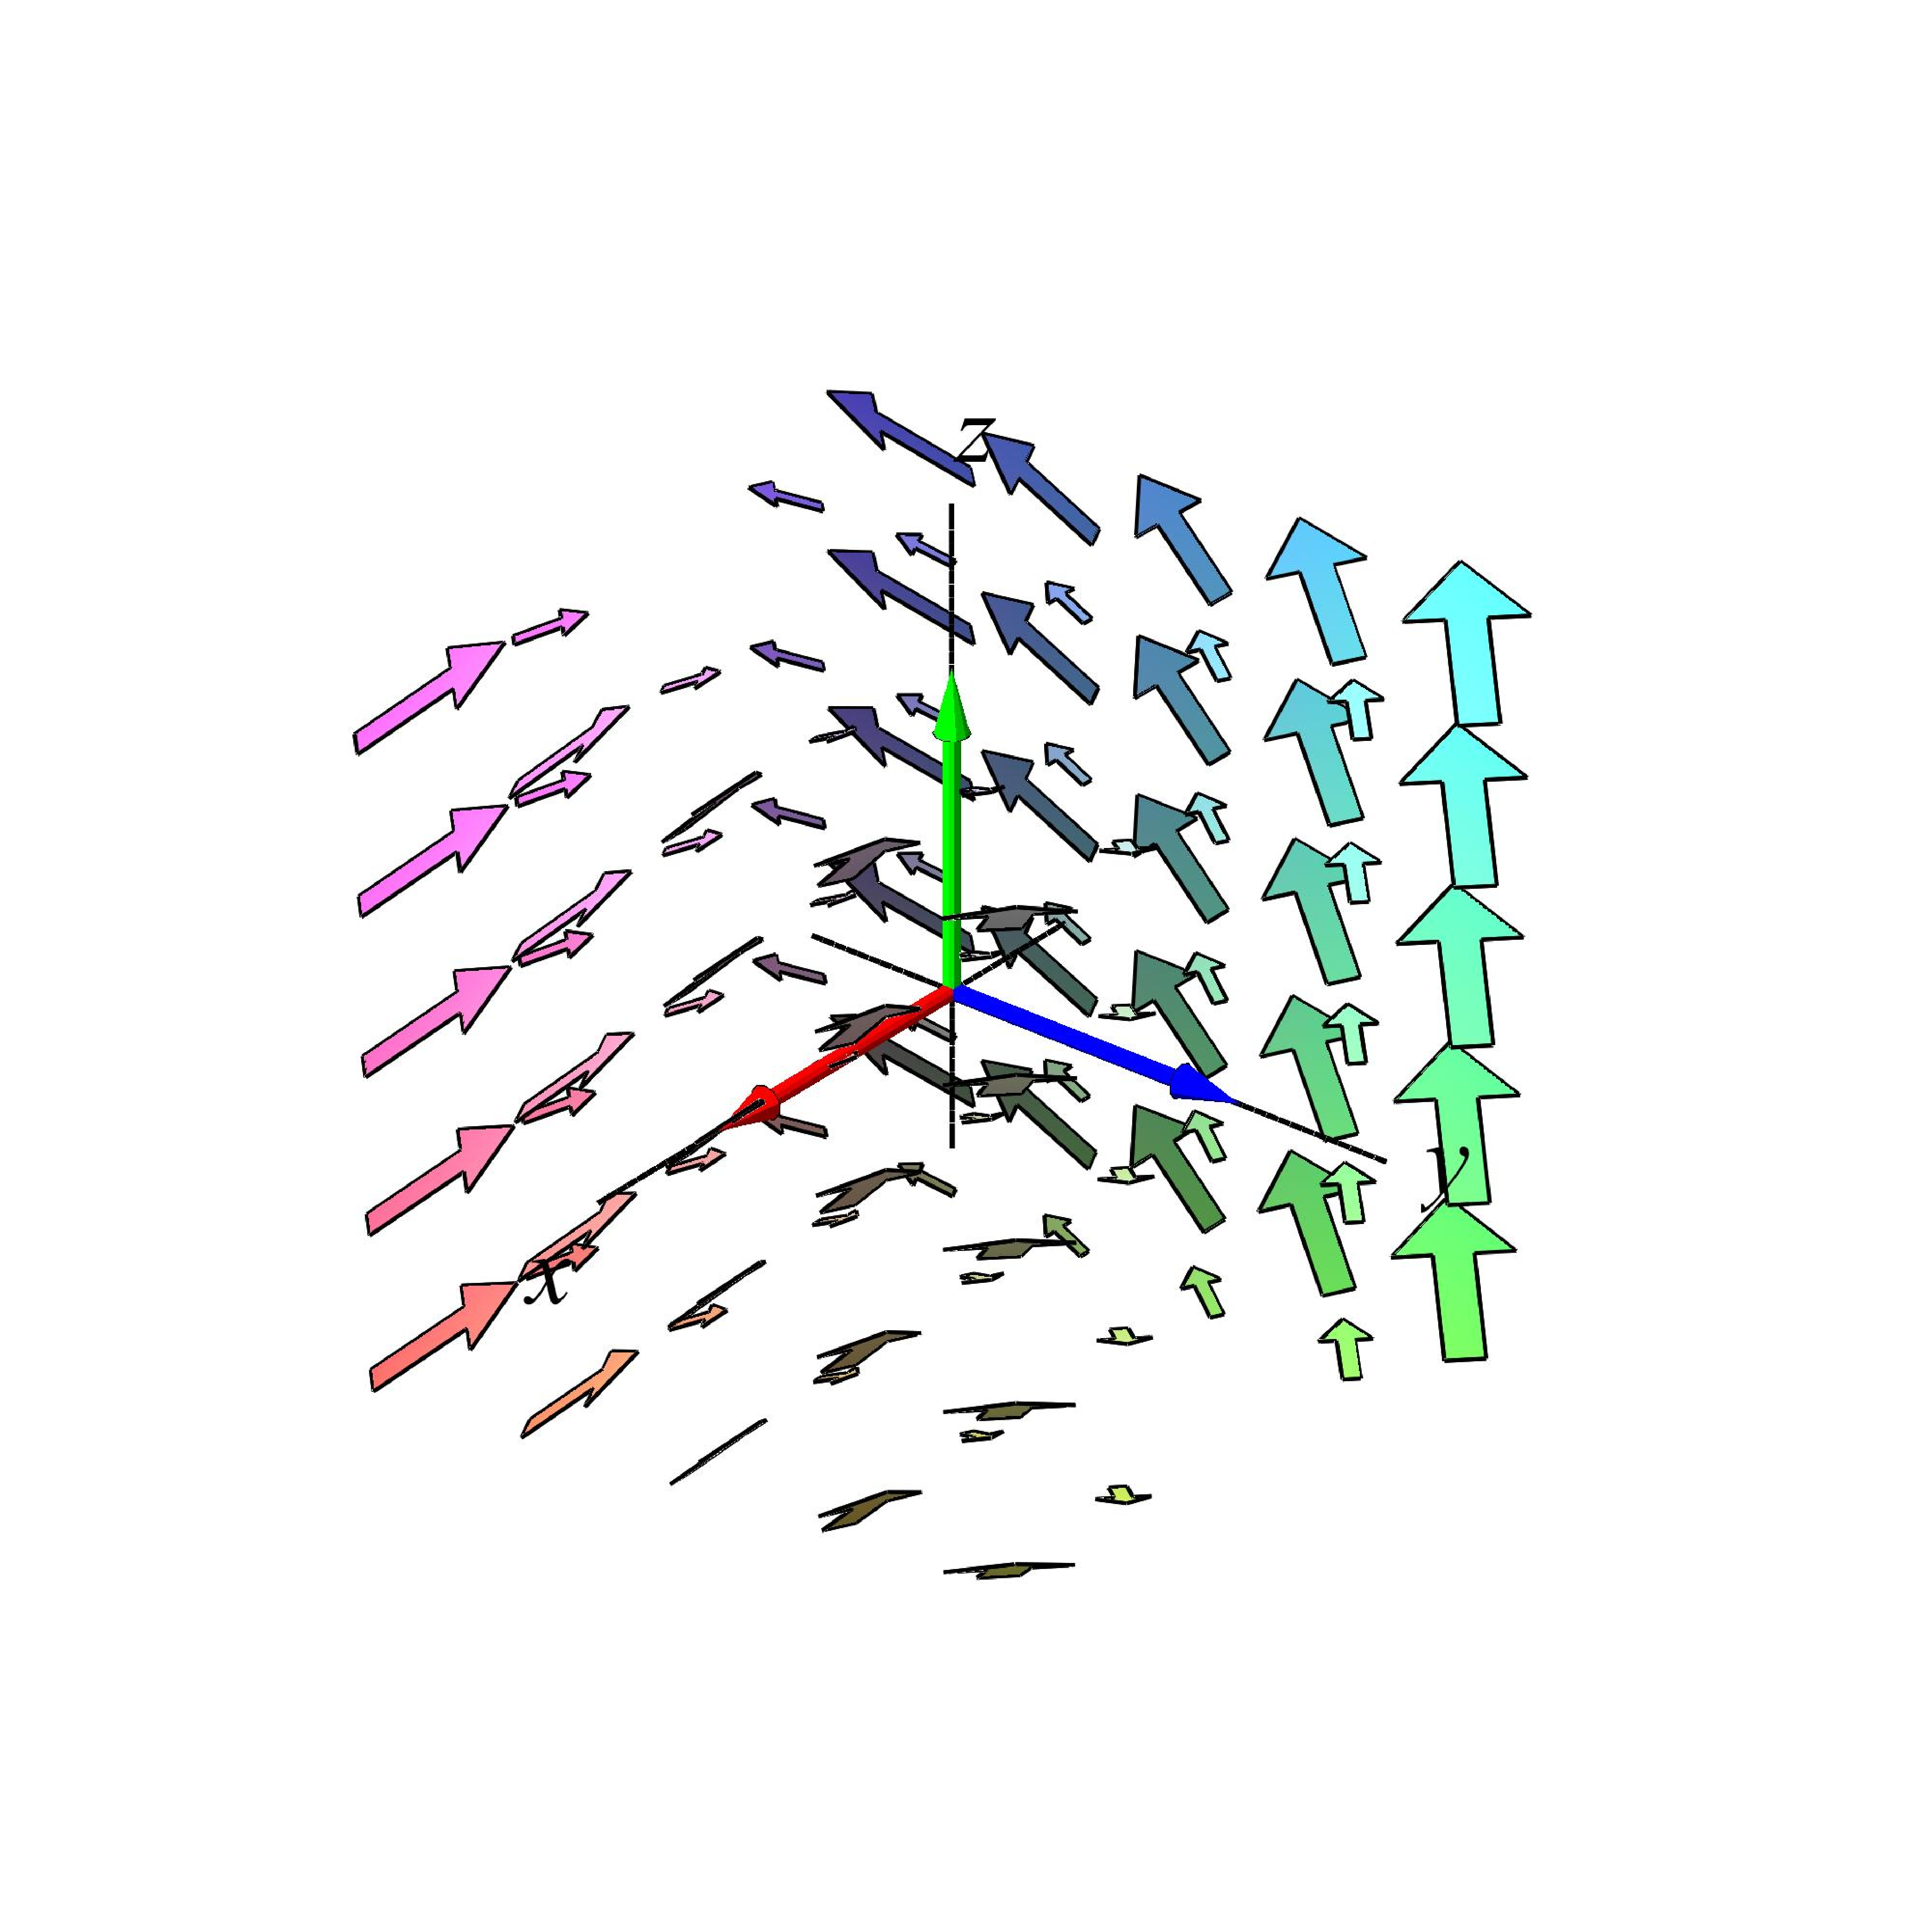
\includegraphics[height=70mm]{FIGS/plotDiskStokes2}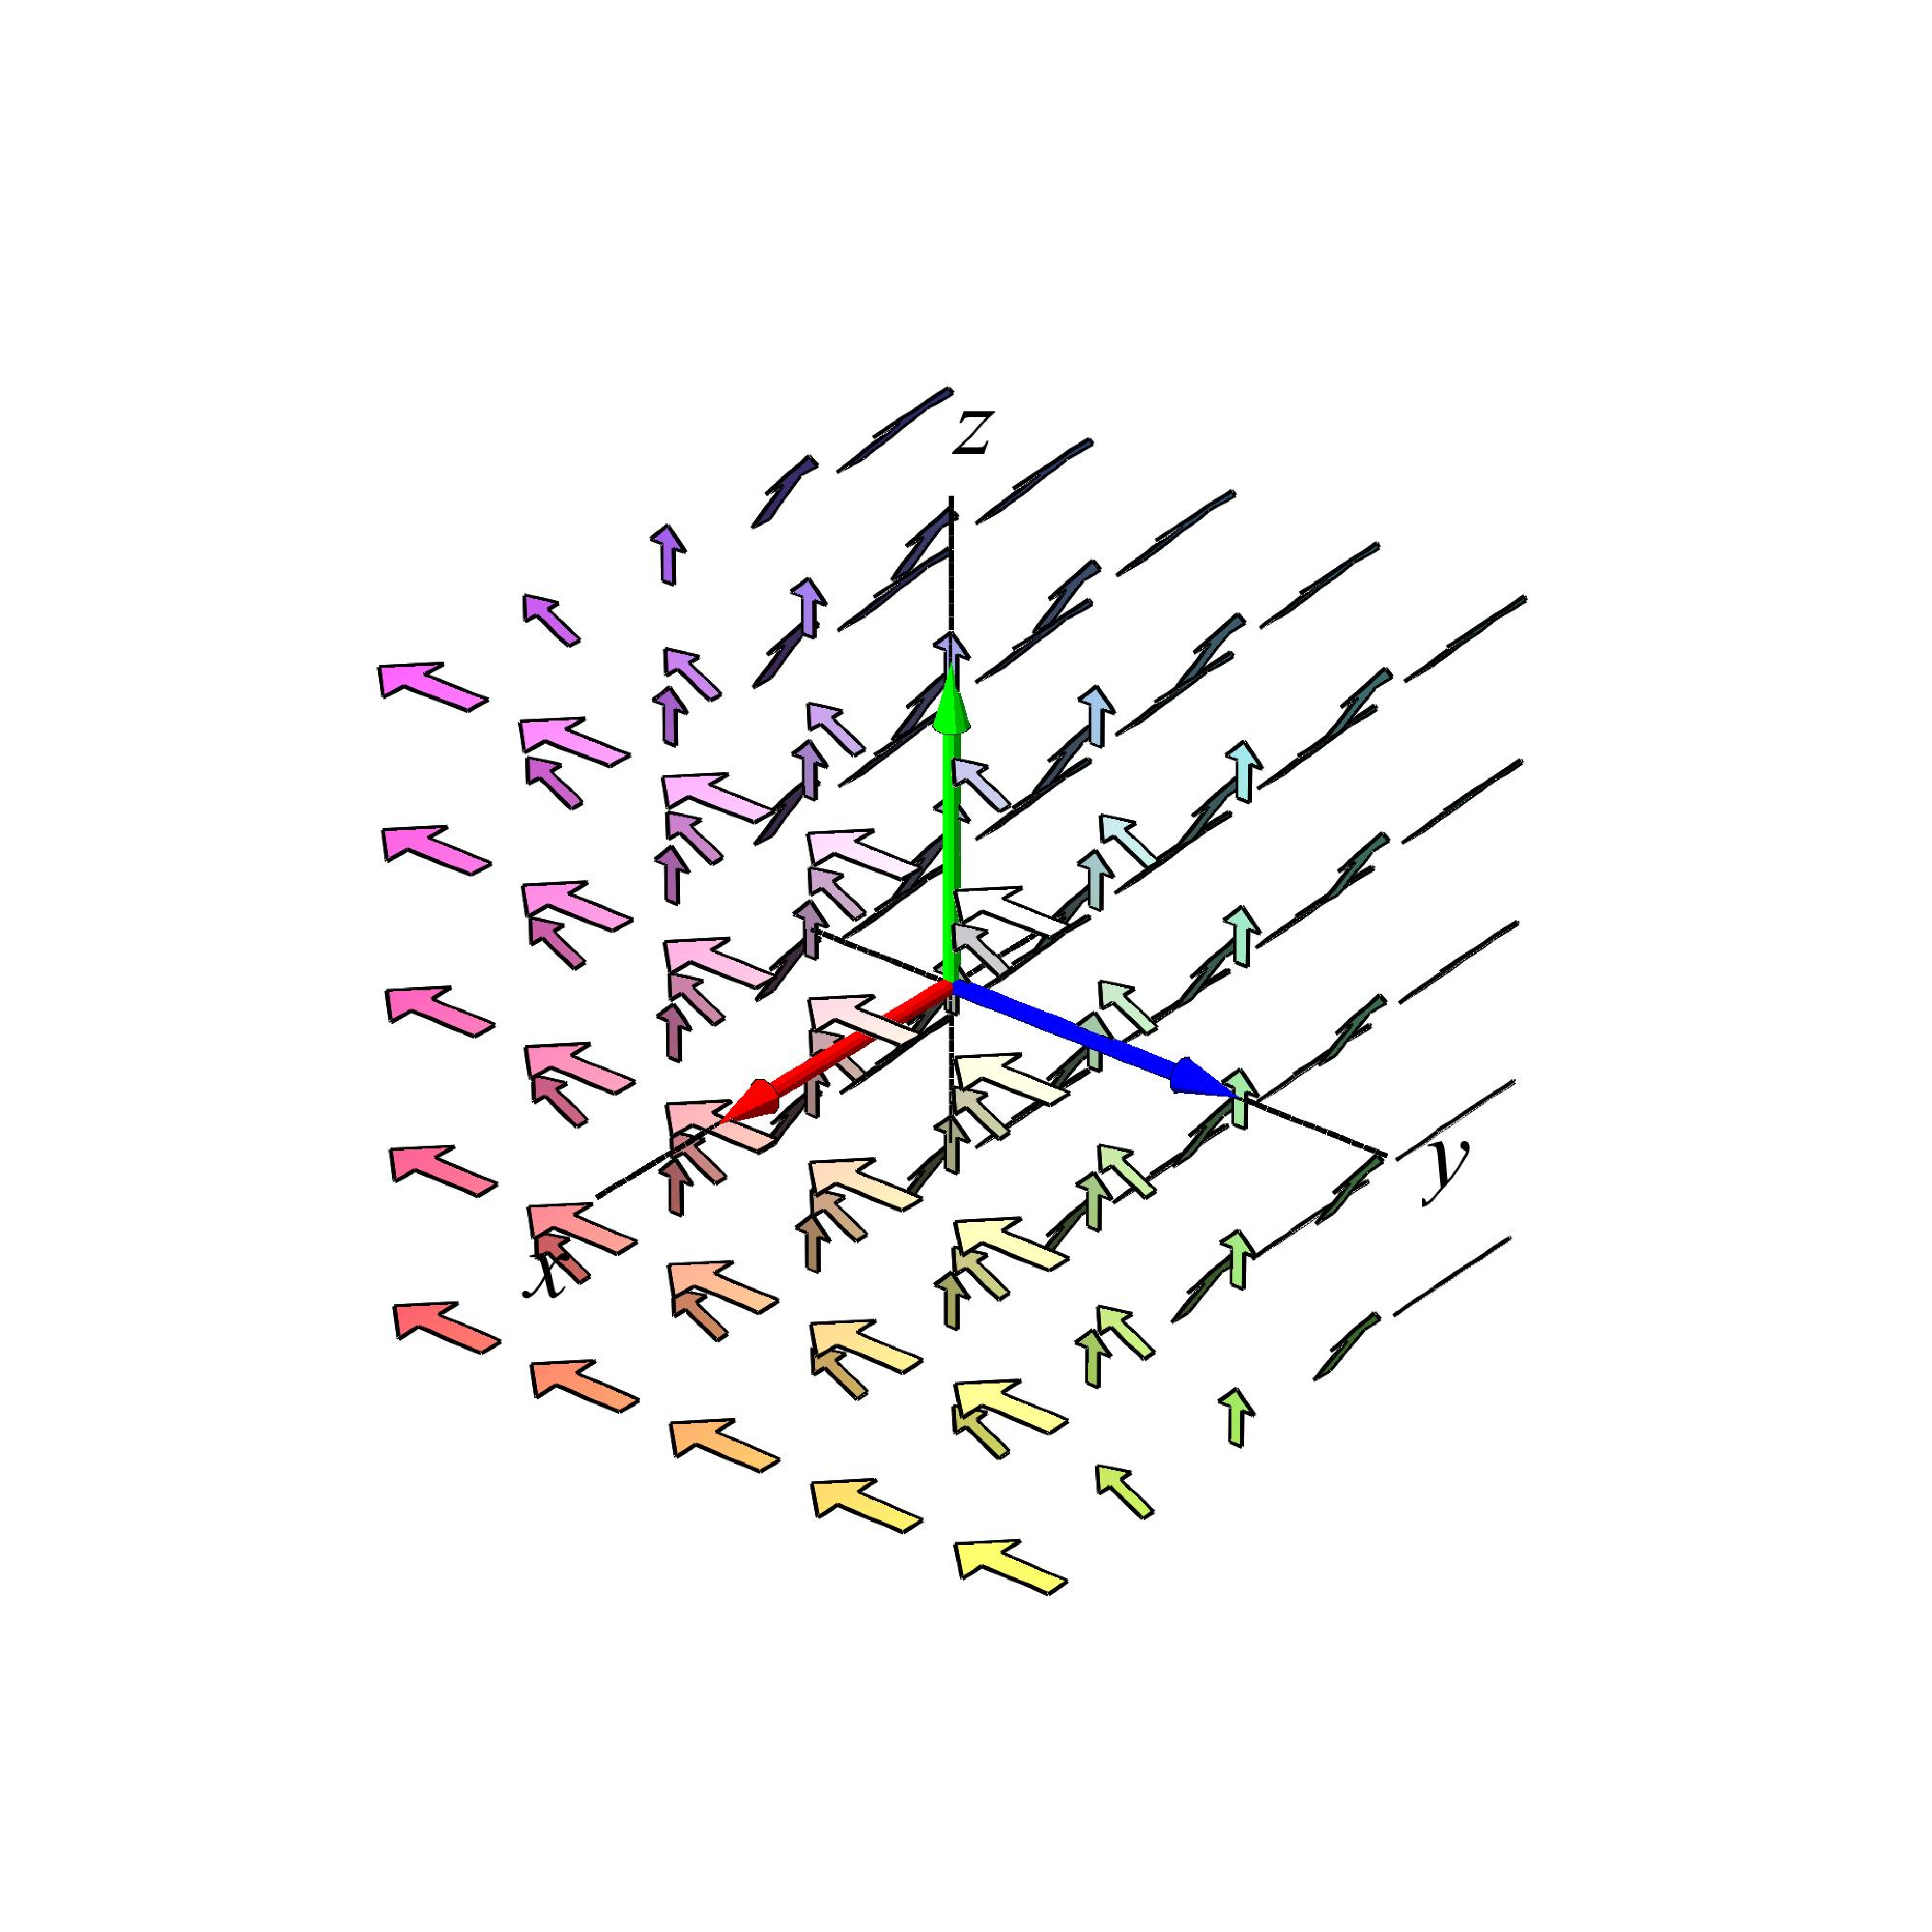
\includegraphics[height=70mm]{FIGS/plotDiskStokes3}}
\begin{center}
\caption{\small{En cirkelskive i et vektorfelt $\mathbf{V}(x,y,z) = (x\cdot y, \, x, \, x^{2})$ (i midten) og  vektorfeltets rotationsvektorfelt  $\Rot(\mathbf{V})(x,y,z)= (0, \, -2\cdot x, \, 1-x)$.}}
\label{figDiskStokesA}
\end{center}
\end{figure}


\begin{figure}[h]
\centerline{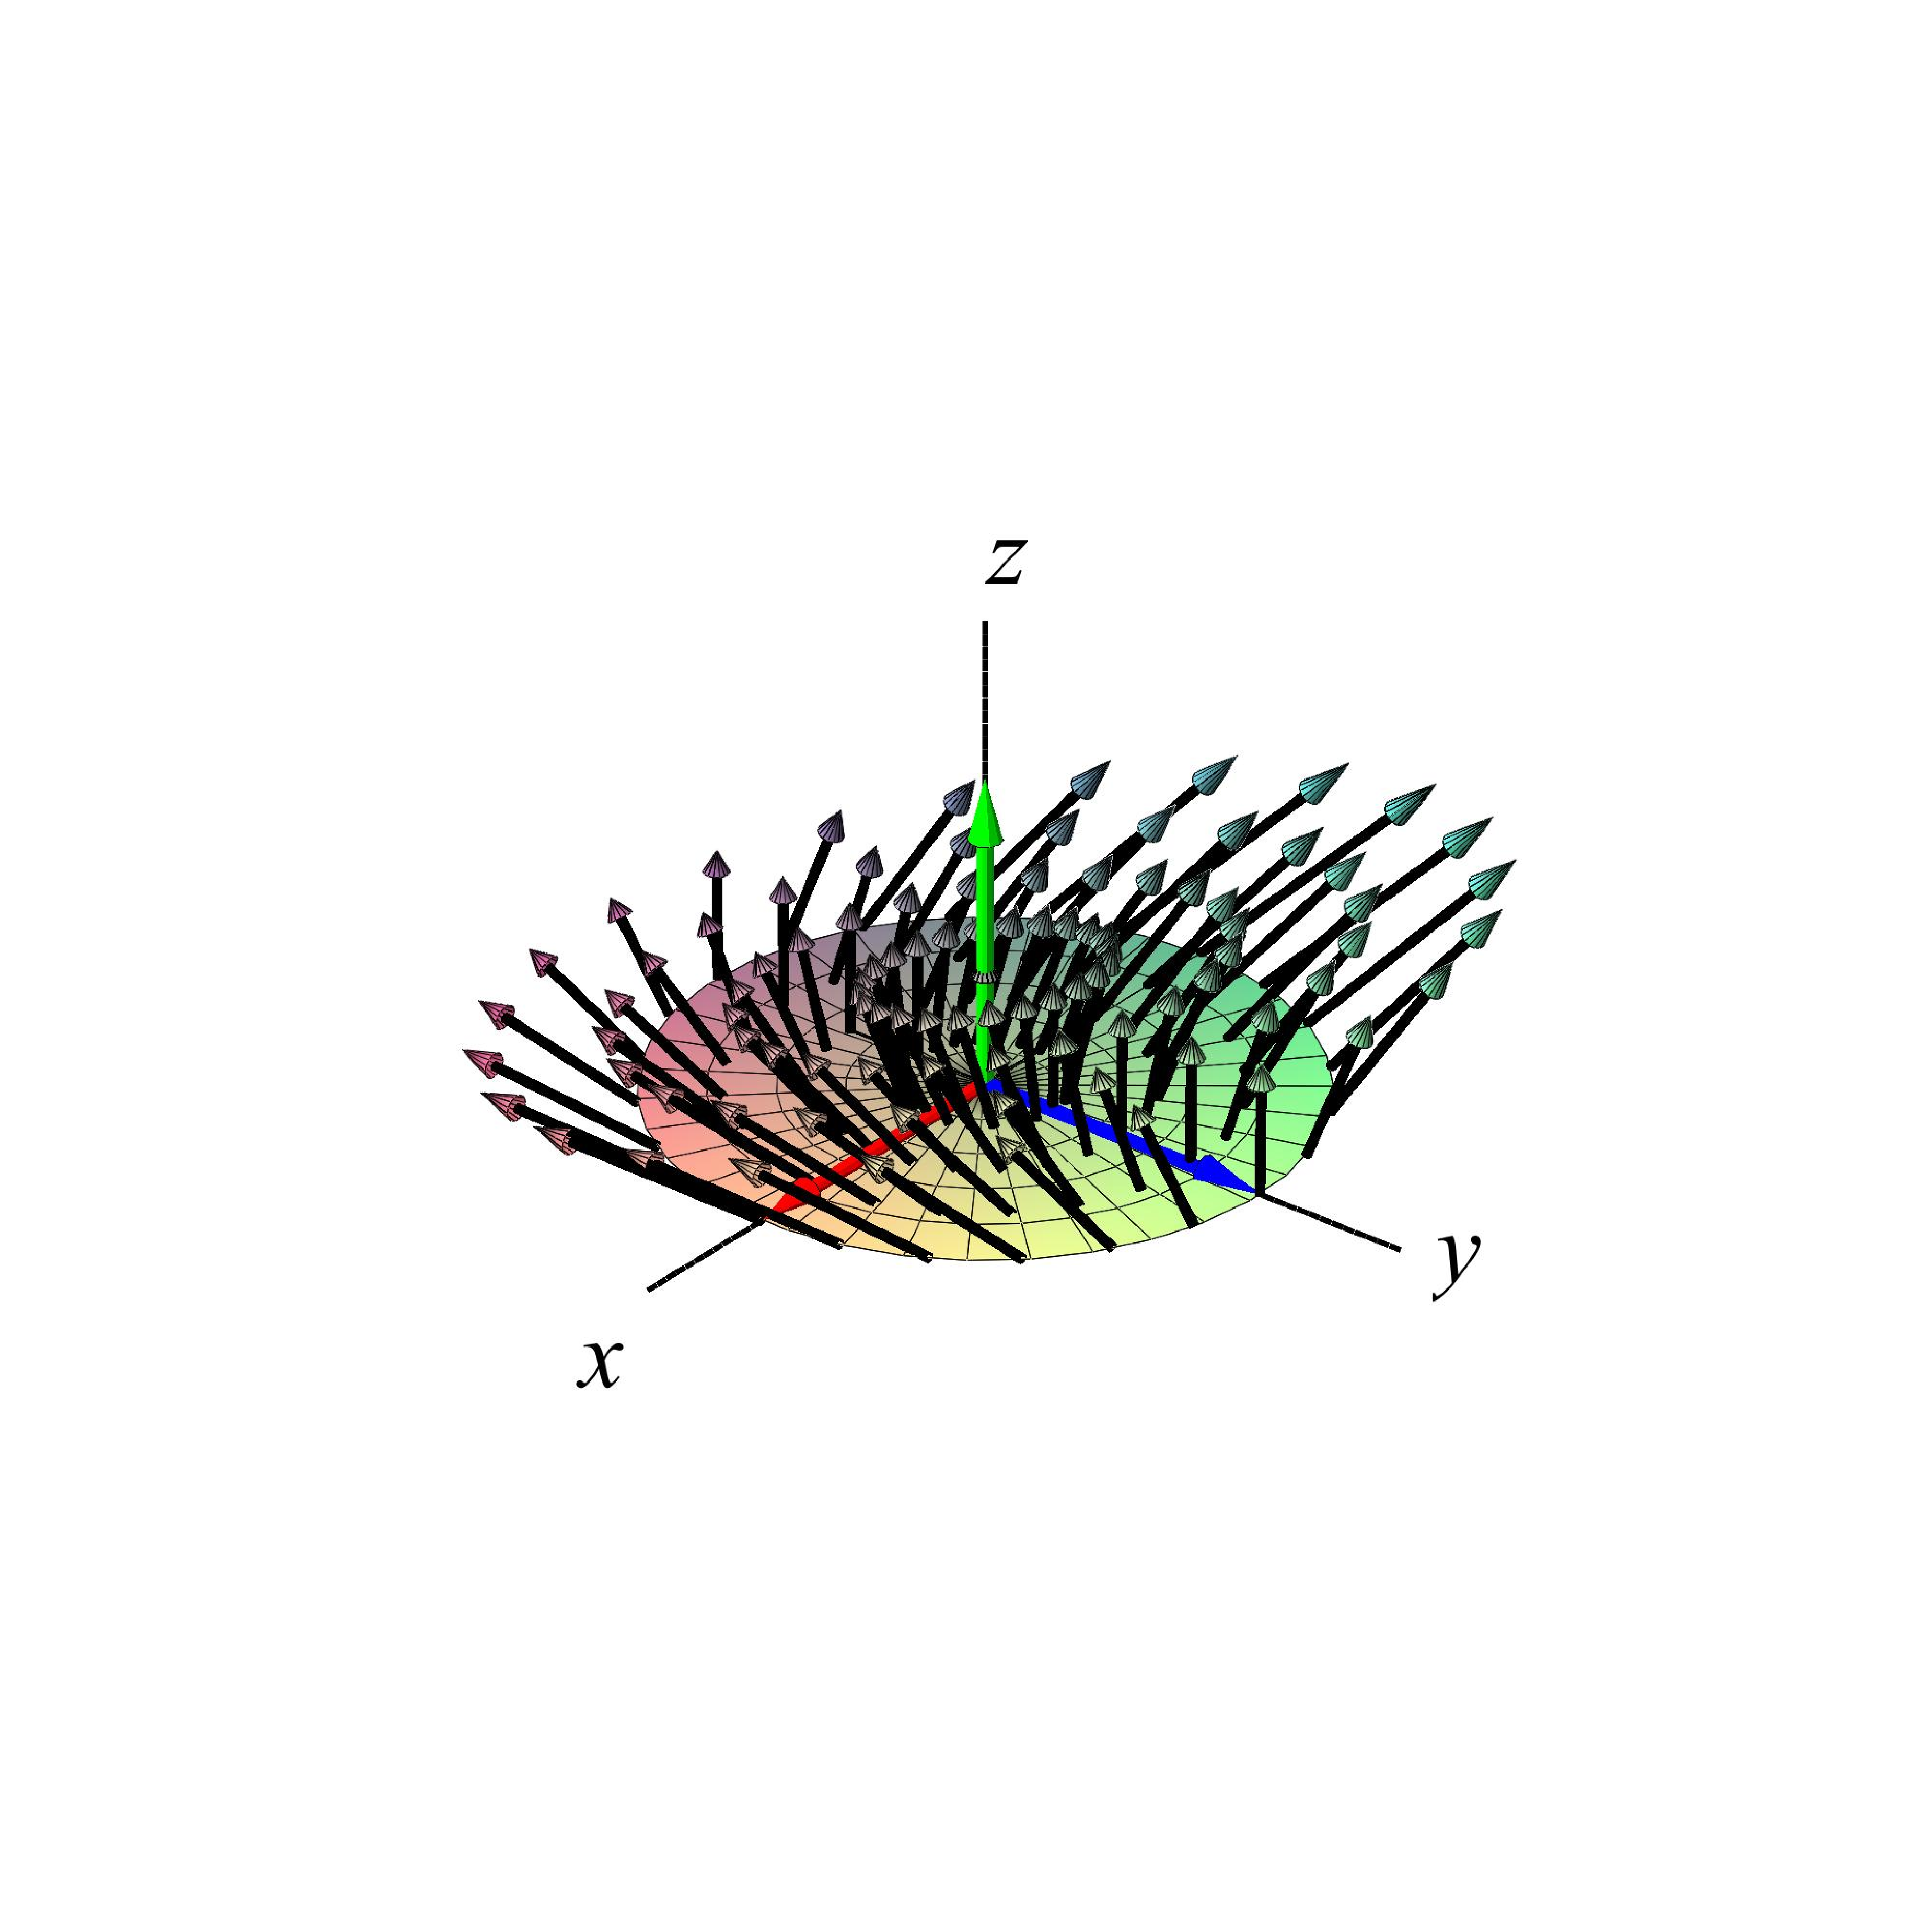
\includegraphics[height=70mm]{FIGS/plotDiskStokes4}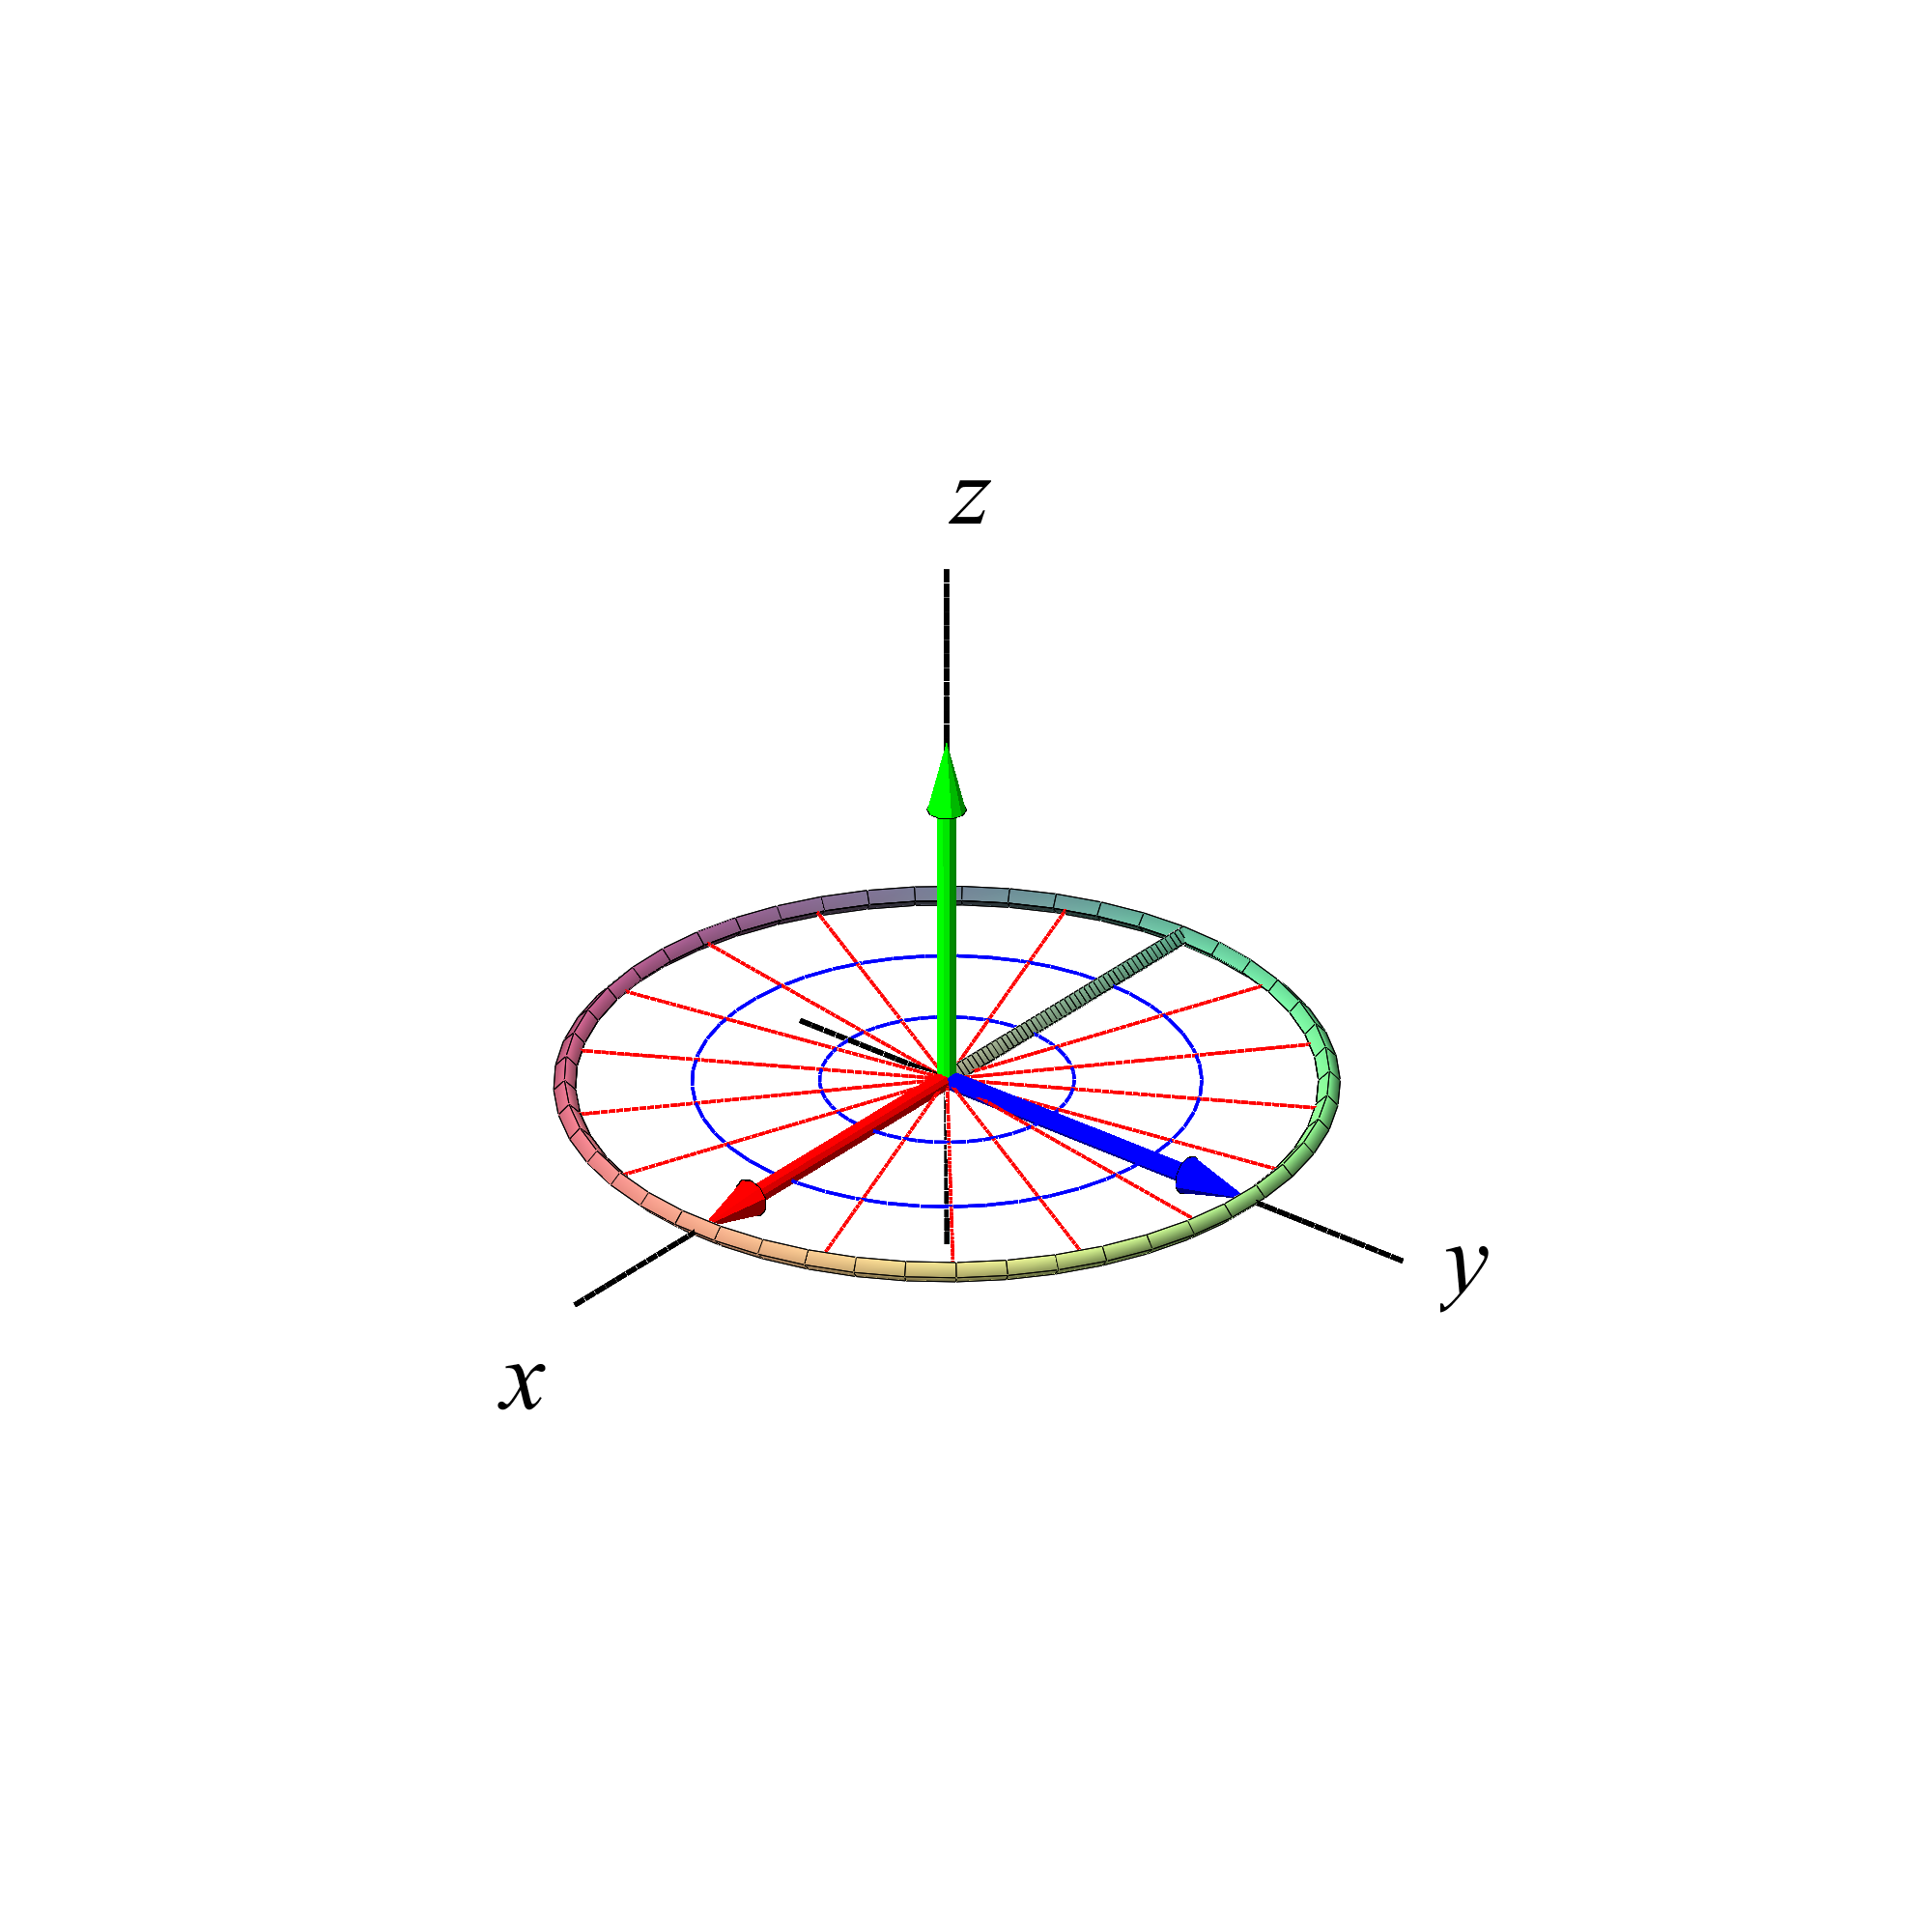
\includegraphics[height=70mm]{FIGS/plotDiskStokes5}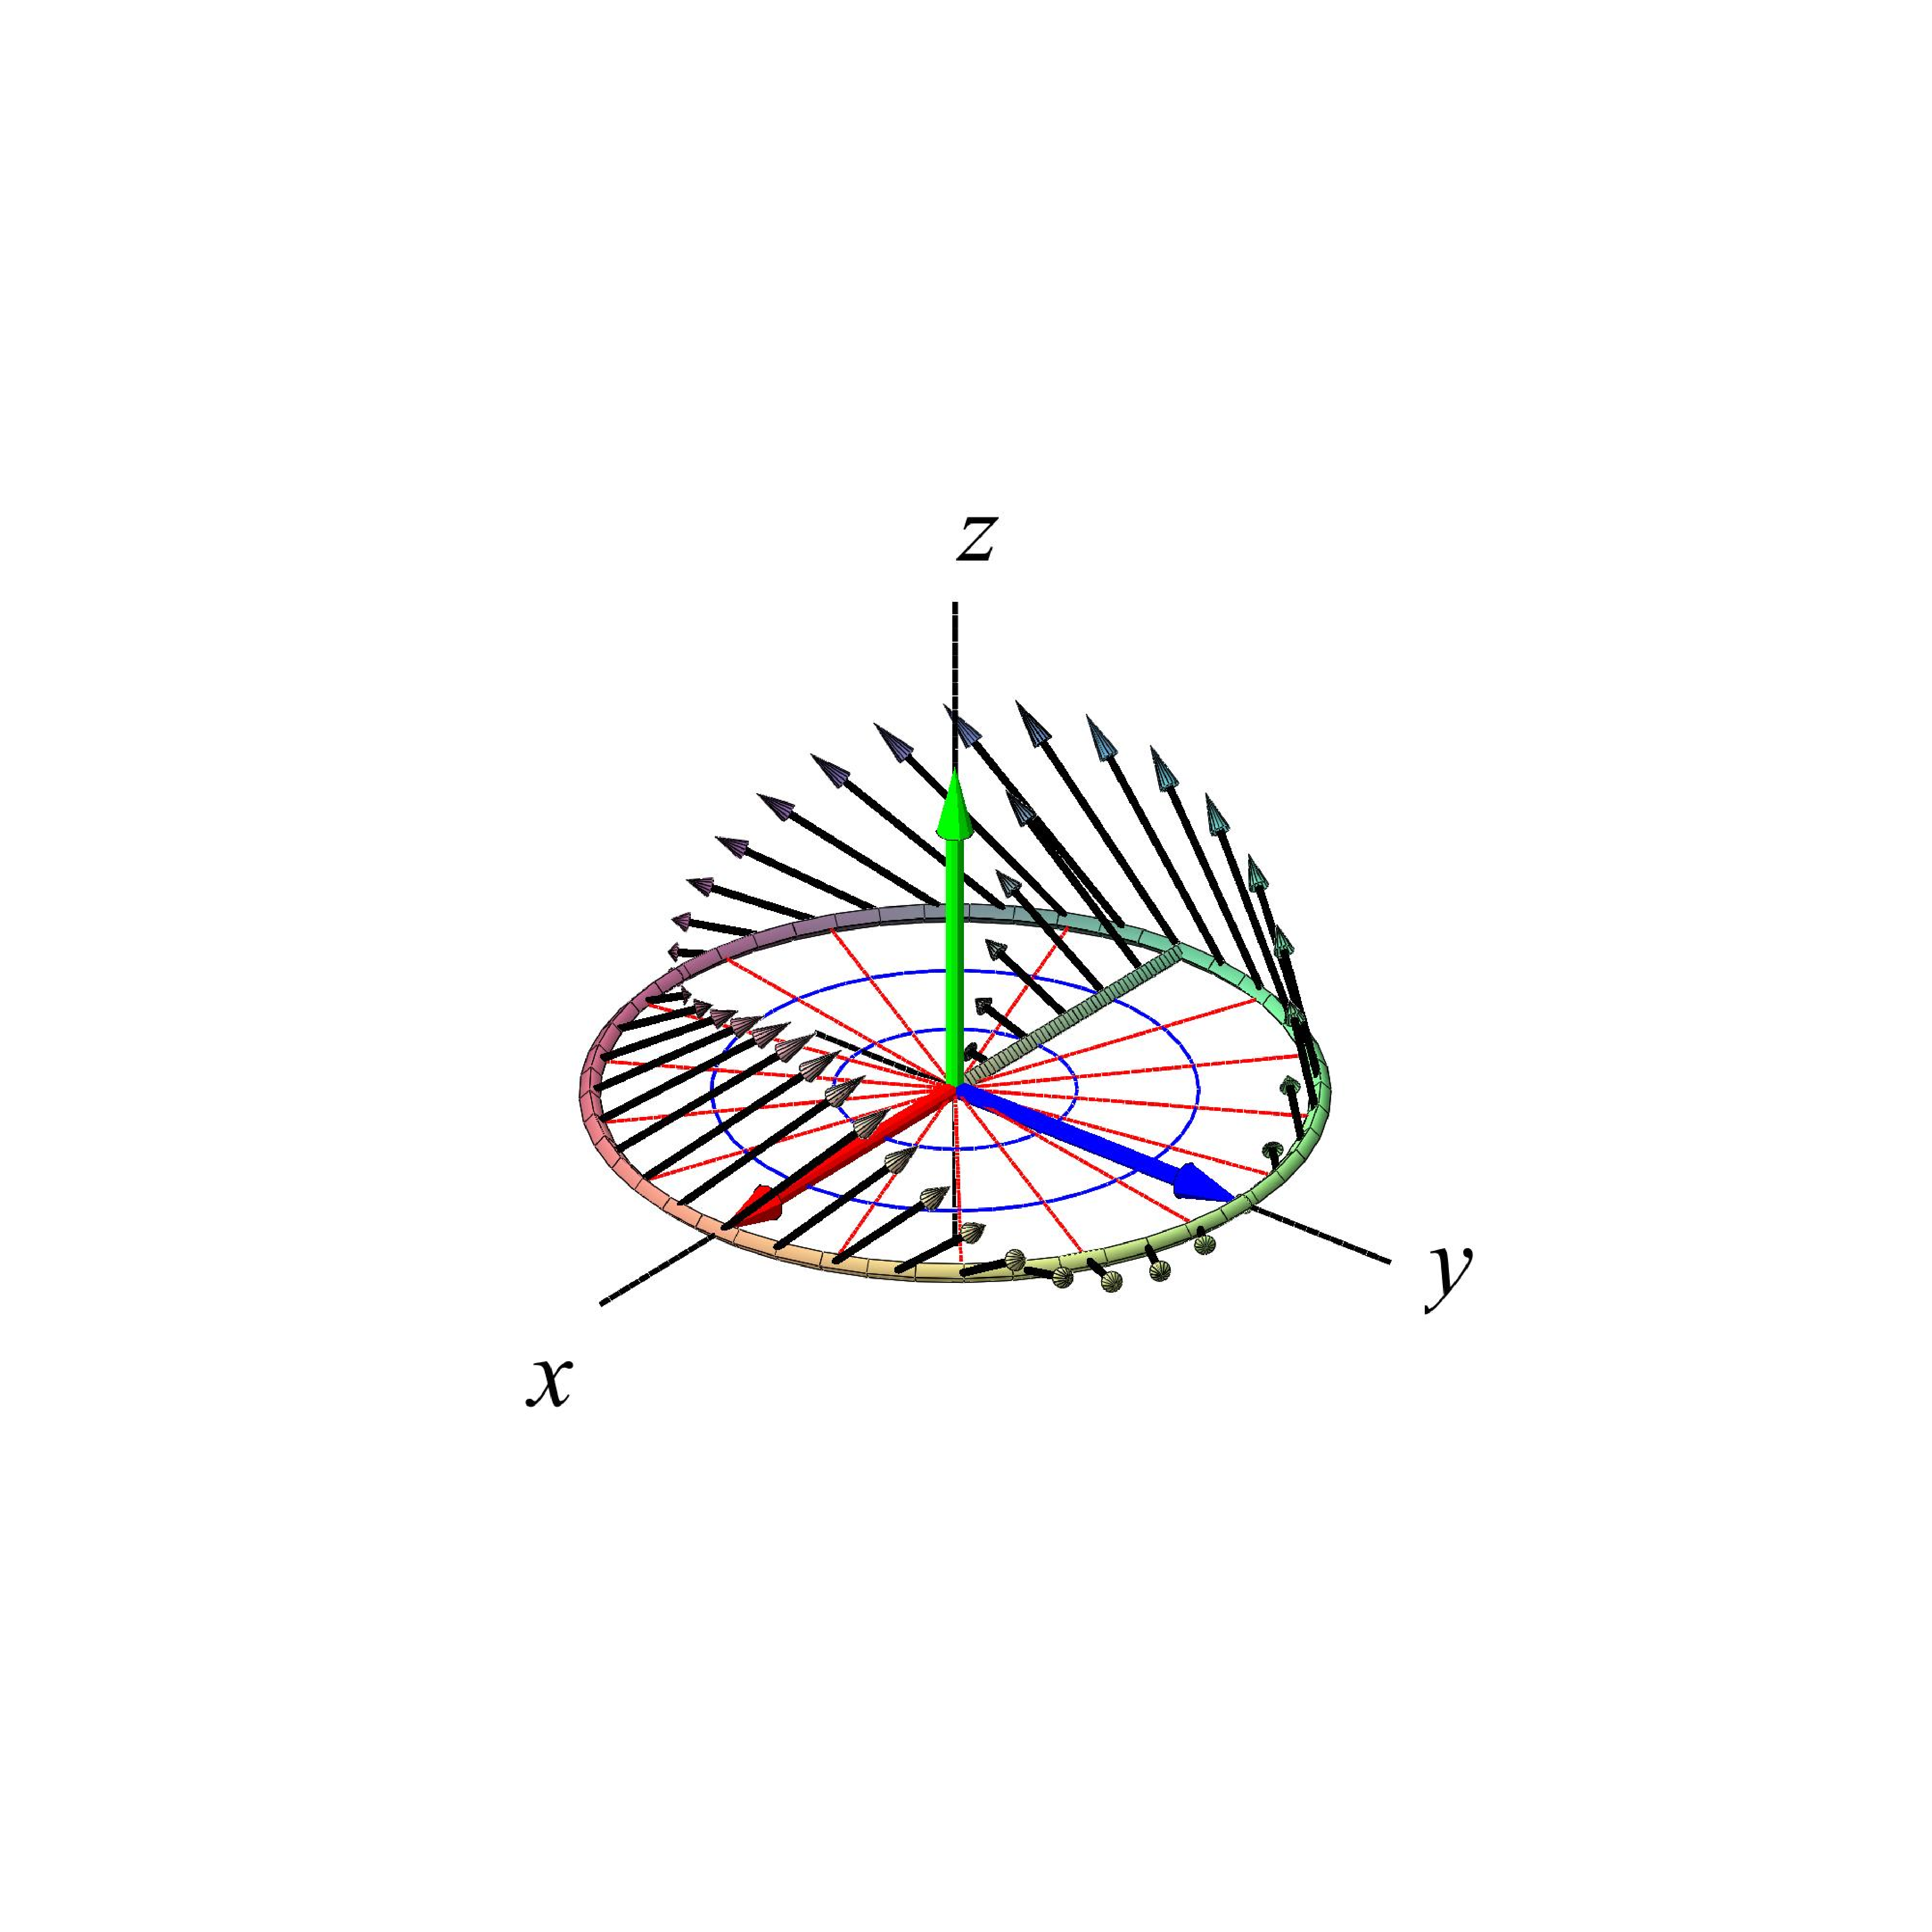
\includegraphics[height=70mm]{FIGS/plotDiskStokes6}}
\begin{center}
\caption{\small{Restriktionen af  rotationsvektorfeltet $\Rot(\mathbf{V})(x,y,z)= (0, \, -2\cdot x, \, 1-x)$ til en cirkelskive, cirkelskivens rand, og vektorfeltet $\mathbf{V}(x,y,z) = (x\cdot y, \, x, \, x^{2})$ restringeret til randen.}}
\label{figDiskStokesB}
\end{center}
\end{figure}



%%%%%%%%%%%%%%%%%%%%%%%%%%%%%%%%%%%%%%%%%%%%%%%%%%%%%%%%%%%%%%%%%%%%%%%%%%%%
%%%%%%%%%%%%%%%%%%%%%%%%%%%%%%%%%%%%%%%%%%%%%%%%%%%%%%%%%%%%%%%%%%%%%%%%%%%%
%%%%%%%%%%%%%%%%%%%%%%%%%%%%%%%%%%%%%%%%%%%%%%%%%%%%%%%%%%%%%%%%%%%%%%%%%%%%
%%%%%%%%%%%%%%%%%%%%%%%%%%%%%%%%%%%%%%%%%%%%%%%%%%%%%%%%%%%%%%%%%%%%%%%%%%%%



%%%%%%%%%%%%%%%%%%%%%%%%%%%%%%%%%%%%%%%%%%%%%%%%%%%%%%%%%%%%%%%%%%%%%%%%%%%%
%%%%%%%%%%%%%%%%%%%%%%%%%%%%%%%%%%%%%%%%%%%%%%%%%%%%%%%%%%%%%%%%%%%%%%%%%%%%
%%%%%%%%%%%%%%%%%%%%%%%%%%%%%%%%%%%%%%%%%%%%%%%%%%%%%%%%%%%%%%%%%%%%%%%%%%%%
%%%%%%%%%%%%%%%%%%%%%%%%%%%%%%%%%%%%%%%%%%%%%%%%%%%%%%%%%%%%%%%%%%%%%%%%%%%%


\begin{example}[Stokes' sætning med en  paraboloide] \label{exampDiskStokes}
Et udsnit af en paraboloide er givet ved en parameterfremstilling således:
\begin{equation}
F_{\mathbf{r}}\quad : \quad \mathbf{r}(u,v) = (2\cdot u \cdot \cos(v), 2\cdot u \cdot \sin(v), u^{2} ) \quad ,
\end{equation}
hvor
\begin{equation}
\quad (u,v) \in [1/2, 1] \times [0, \pi]
\end{equation}
Parameterfremstillingen har  Jacobifunktionen
\begin{equation}
\Jac_{\mathbf{r}}(u,v) = 4\cdot u \cot \sqrt{1 + u^{2}} \quad ,
\end{equation}
og standard-normalvektorfeltet (ikke nødvendigvis enheds-vektorer)  til fladen er givet ved
\begin{equation}
\mathbf{N}_{F}(u,v) = \mathbf{r}'_{u}(u,v) \times \mathbf{r}'_{v}(u,v) = (-4\cdot u^{2}\cdot \cos(v), \, -4\cdot u^{2}\cdot \sin(v), \,4\cdot u) \quad .
\end{equation}
Et glat vektorfelt i rummet er givet ved sine koordinatfunktioner således:
\begin{equation}
\mathbf{V}(x,y,z) = (z, y, -x) \quad ,
\end{equation}
med det tilhørende rotationsvektorfelt
\begin{equation}
\Rot(\mathbf{V})(x,y,z) = (0\, , \, 2 \, , \, 0) \quad .
\end{equation}
Vi vil verificere Stokes' sætning ved at beregne ''begge sider'' af ligning (\ref{eqStokes}) i dette konkrete tilfælde.\\

Den totale flux af vektorfeltet $\Rot(\mathbf{V})(x,y,z)$ igennem $F_{\mathbf{r}}$ i retning af standard-enhedsnormalen er, idet vi benytter
normalvektorfeltet $\mathbf{N}_{F}(u,v)$ direkte:
\begin{equation}
\begin{aligned}
\Flux(\Rot(\mathbf{V}), F_{\mathbf{r}} ) &= \int_{F_{\mathbf{r}}}\Rot(\mathbf{V}) \bm{\cdot} \mathbf{n}_{F} \, d\mu \\
&= \int_{0}^{\pi}\int_{1/2}^{1} \Rot(\mathbf{V}) \bm{\cdot} \mathbf{N}_{F}(u,v) \, du \, dv \\
&=  \int_{0}^{\pi}\int_{1/2}^{1} \left(-8\cdot u^{2} \cdot \sin(v) \right)  \, du \, dv \\
&= \int_{0}^{\pi} \left( \frac{-7}{3} \cdot \sin(v) \right)\, dv \\
&= \frac{-14}{3}\quad .
\end{aligned}
\end{equation}
Cirkulationen af vektorfeltet $\mathbf{V}(x,y,z)$ langs $\partial F_{\mathbf{r}}$ i retning af den korrekt orienterede randkurve består af fire
komponenter. De fås fra fladens parameterfremstilling $\mathbf{r}(u,v)$ dels ved at fastholde $v$ til at være henholdsvis $0$ og $\pi$, og dels ved at fastholde $u$ til at være henholdsvis $1/2$ og $1$,  idet det i hvert tilfælde samtidigt sikres, at den frie parameter løber den 'rigtige vej', dvs. således at alle fire randkomponenter får den rette orientering i forhold til fladens normalvektorfelt:
\begin{equation}
\begin{aligned}
\partial_{1} F \quad : \quad \mathbf{r}_{1}(u) &= \mathbf{r}(u, 0) = (2\cdot u , \, 0 , \, u^{2}) \quad , \quad  u \in [1/2, \, 1] \\
\mathbf{r}'_{1}(u) &= (2, \, 0, \, 2\cdot u)\\
\mathbf{V}(\mathbf{r}_{1}(u)) &= (u^{2},\, 0, \, -2\cdot u) \\
\mathbf{r}'_{1}(u)\cdot \mathbf{V}(\mathbf{r}_{1}(u)) &= -2\cdot u^{2} \quad ,
\end{aligned}
\end{equation}

\begin{equation}
\begin{aligned}
\partial_{3} F \quad : \quad \mathbf{r}_{3}(u) &= \mathbf{r}(1 - u + 1/2, v) = (-3 + 2 \cdot u, \, 0, \, (-3/2 + u)^{2})\quad , \quad  u \in [1/2, \, 1] \\
\mathbf{r}'_{3}(u) &= (2, \, 0 , \, 2\cdot u - 3) \\
\mathbf{V}(\mathbf{r}_{3}(u)) &= ((-3/2 + u)^{2}, \, 0, \, 3 - 2\cdot u)  \\
\mathbf{r}'_{3}(u)\cdot \mathbf{V}(\mathbf{r}_{3}(u)) &= \frac{-9}{2} + 6\cdot u - 2\cdot u^{2} \quad ,
\end{aligned}
\end{equation}

\begin{equation}
\begin{aligned}
\partial_{2} F \quad : \quad \mathbf{r}_{2}(v) &= \mathbf{r}(1, v) = (2\cdot \cos(v), \, 2\cdot \sin(v), \, 1) \quad , \quad  v \in [0, \, \pi] \\
\mathbf{r}'_{2}(v) &= (-2\cdot \sin(v), \, 2 \cdot \cos(v), \, 0) \\
\mathbf{V}(\mathbf{r}_{2}(v)) &= (1, \, 2\cdot \sin(v), \, -2\cdot \cos(v)) \\
\mathbf{r}'_{2}(v)\cdot \mathbf{V}(\mathbf{r}_{2}(v)) &= 2\cdot \sin(v)\cdot  \left(2\cdot \cos(v) -1 \right) \quad , \end{aligned}
\end{equation}

\begin{equation}
\begin{aligned}
\partial_{4} F \quad : \quad \mathbf{r}_{4}(v) &= \mathbf{r}(1/2, \, \pi - v) = (-\cos(v), \sin(v), 1/4) \quad , \quad  v \in [0, \, \pi] \\
\mathbf{r}'_{4}(v) &= (\sin(v), \, \cos(v) , \, 0) \\
\mathbf{V}(\mathbf{r}_{4}(v)) &= (\frac{1}{4}, \, \sin(v), \, \cos(v))  \\
\mathbf{r}'_{4}(v)\cdot \mathbf{V}(\mathbf{r}_{4}(v)) &= \frac{1}{4}\cdot \sin(v)\cdot  \left(\cos(v) +1 \right)  \quad .
\end{aligned}
\end{equation}

Vi har dermed følgende totale cirkulation af $\mathbf{V}(x,y,z)$ langs randen:
\begin{equation}
\begin{aligned}
\operatorname{Cirk}(\mathbf{V}, \partial F) &= \sum_{i=1}^{4} \operatorname{Cirk}(\mathbf{V}, \partial_{i} F) \\
&= \sum_{i=1}^{4} \int_{\partial_{i} F} \mathbf{V}(\mathbf{r}_{i}(t))\cdot \mathbf{r}'_{i}(t) \, \, dt \\
&= \int_{1/2}^{1} \left(-2\cdot u^{2}\right) \,\, du \\
&\phantom{abc}+ \int_{1/2}^{1} \left(\frac{-9}{2} + 6\cdot u - 2\cdot u^{2}\right) \,\, du \\
&\phantom{abcdef}+ \int_{0}^{\pi} 2\cdot \sin(v)\cdot  \left(2\cdot \cos(v) -1 \right) \,\, dv \\
&\phantom{abcdefghi}+ \int_{0}^{\pi} \frac{1}{4}\cdot \sin(v)\cdot  \left(\cos(v) +1 \right)\,\, dv \\
&= - \frac{7}{12} -  \frac{7}{12} - 4 + \frac{1}{2} = - \frac{14}{3} \quad .
\end{aligned}
\end{equation}
Begge sider i ligningen (\ref{eqStokes}) giver altså $-14/3$ i dette eksempel, og vi har således igen verificeret Stokes' sætning.
\end{example}



\begin{figure}[h]
\centerline{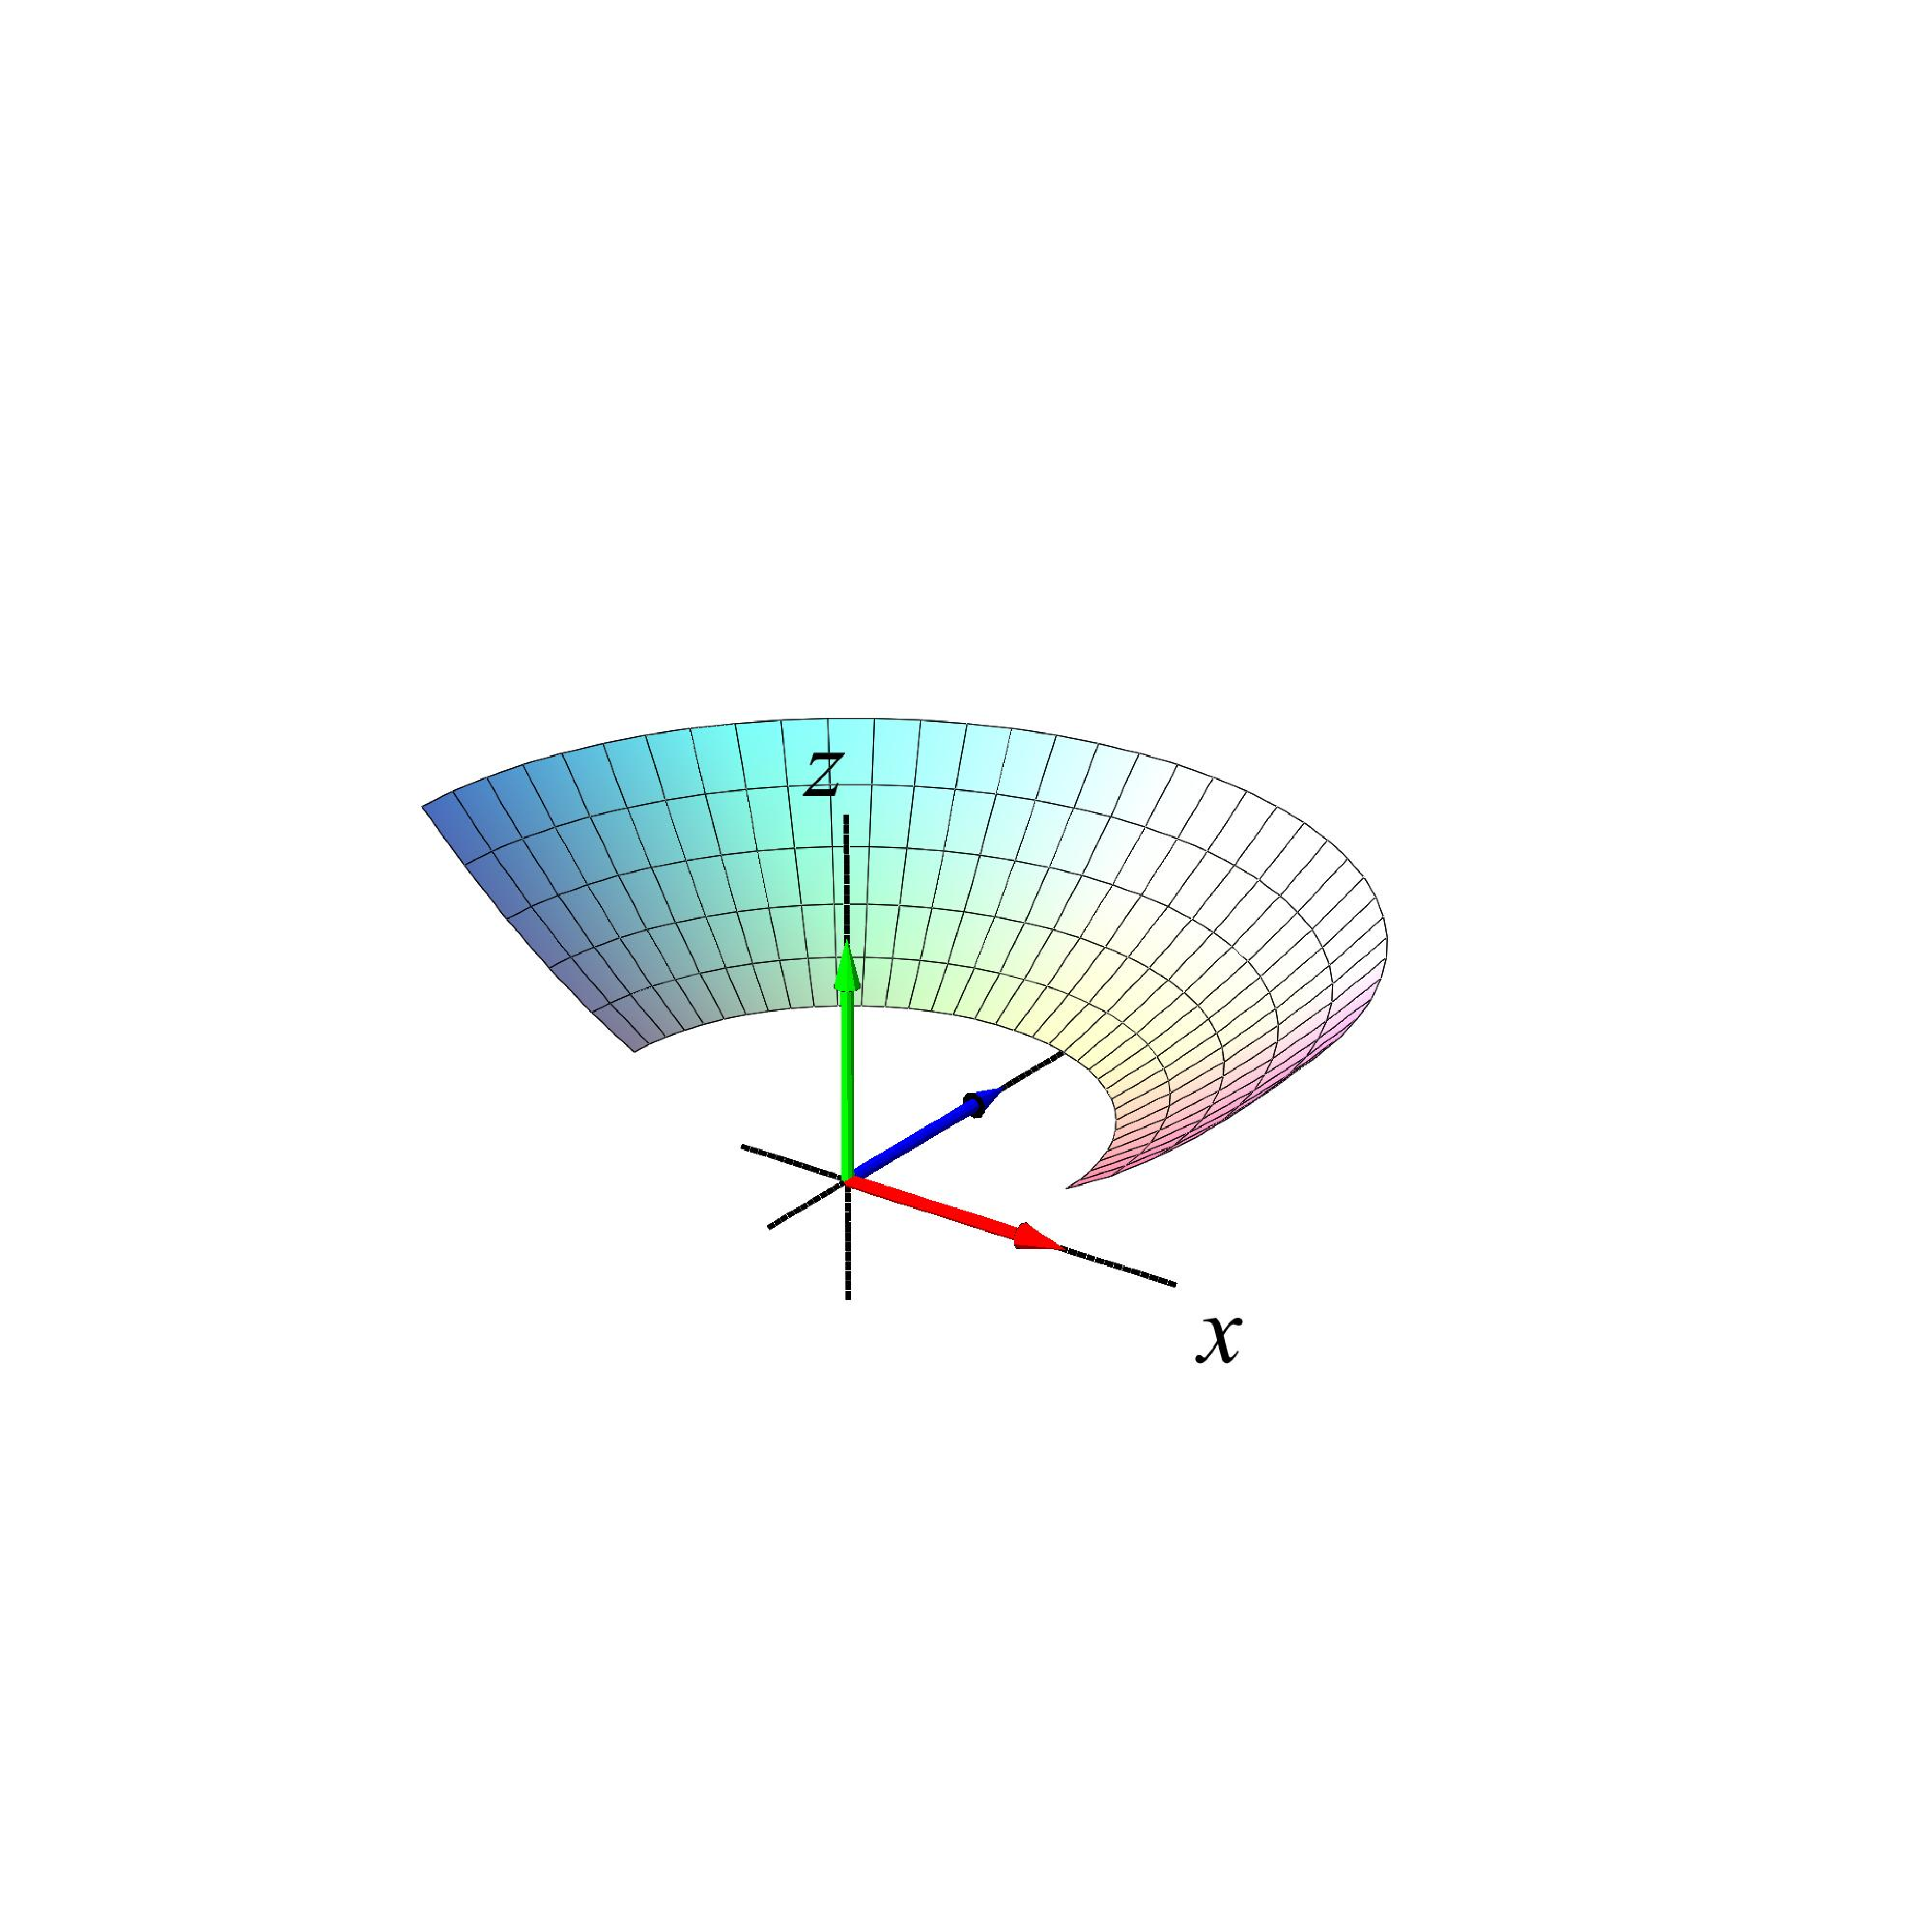
\includegraphics[height=70mm]{FIGS/plotParab1}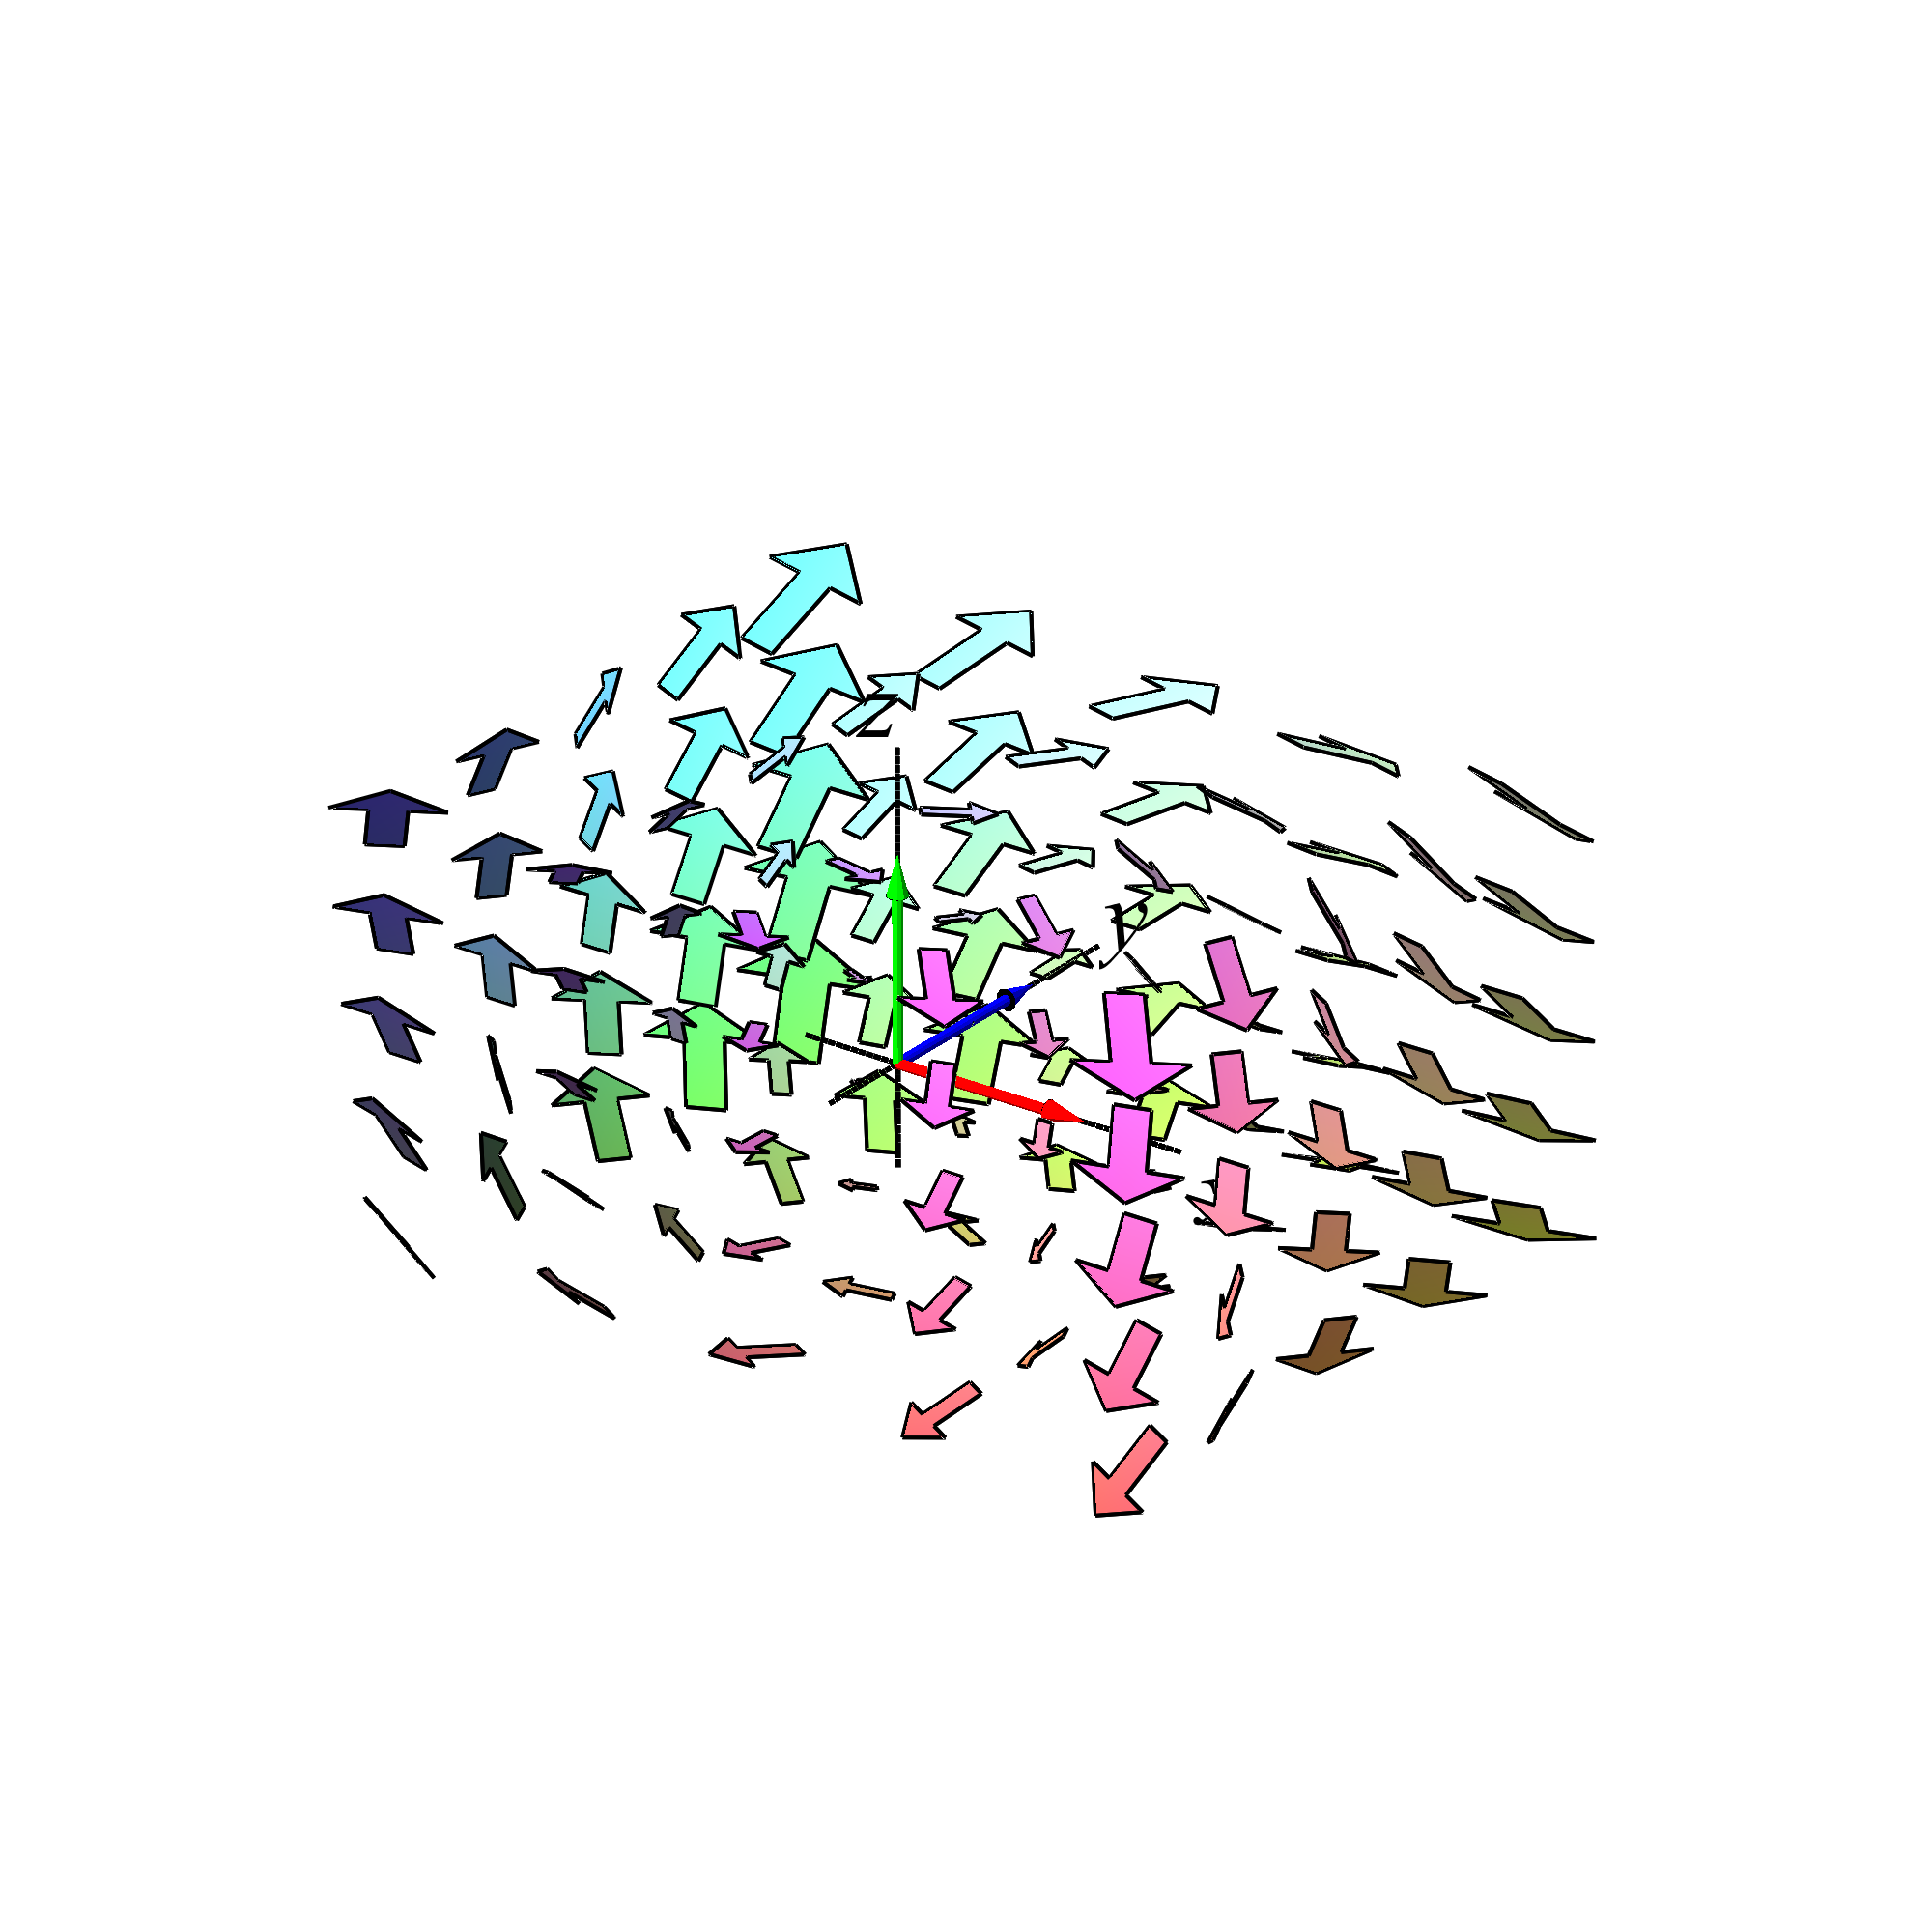
\includegraphics[height=70mm]{FIGS/plotParab2}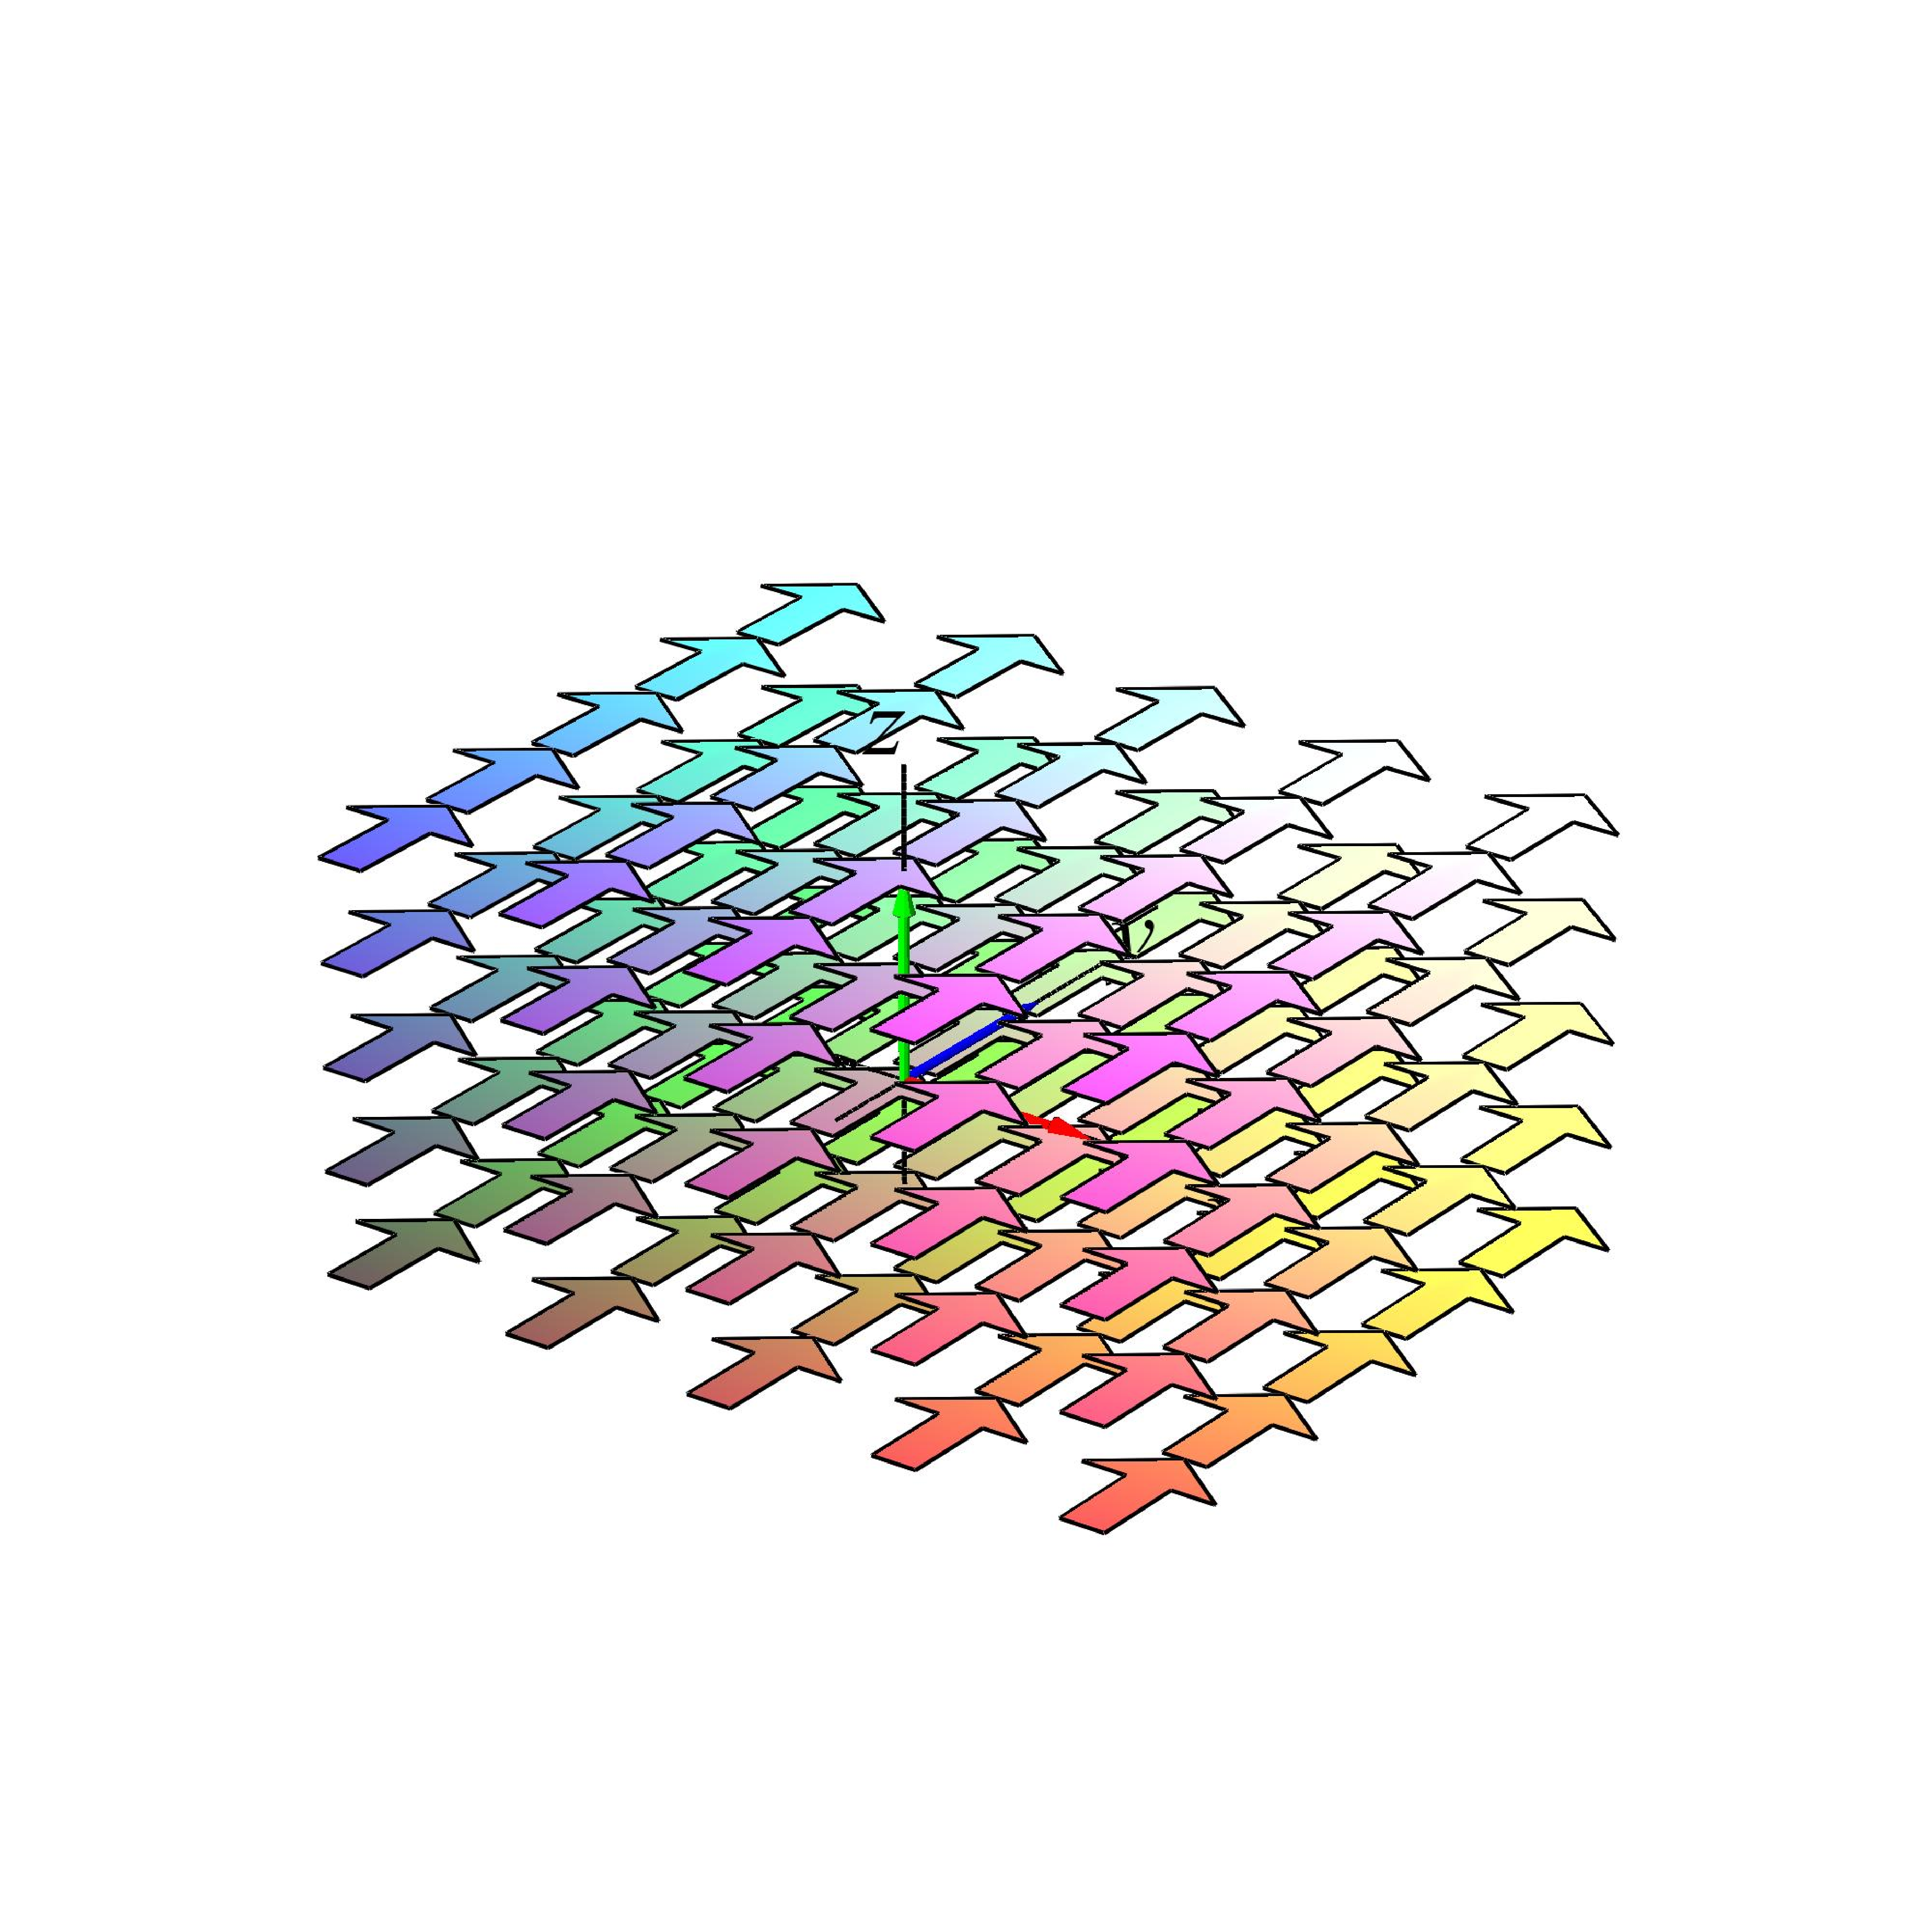
\includegraphics[height=70mm]{FIGS/plotParab3}}
\begin{center}
\caption{\small{Et stykke af en paraboloide i et vektorfelt $\mathbf{V}(x,y,z) = (z, \,y, \, -x)$ (i midten) og  vektorfeltets rotationsvektorfelt  $\Rot(\mathbf{V})(x,y,z)= (0, \, 2, \, 0)$.}}
\label{figParabA}
\end{center}
\end{figure}


\begin{figure}[h]
\centerline{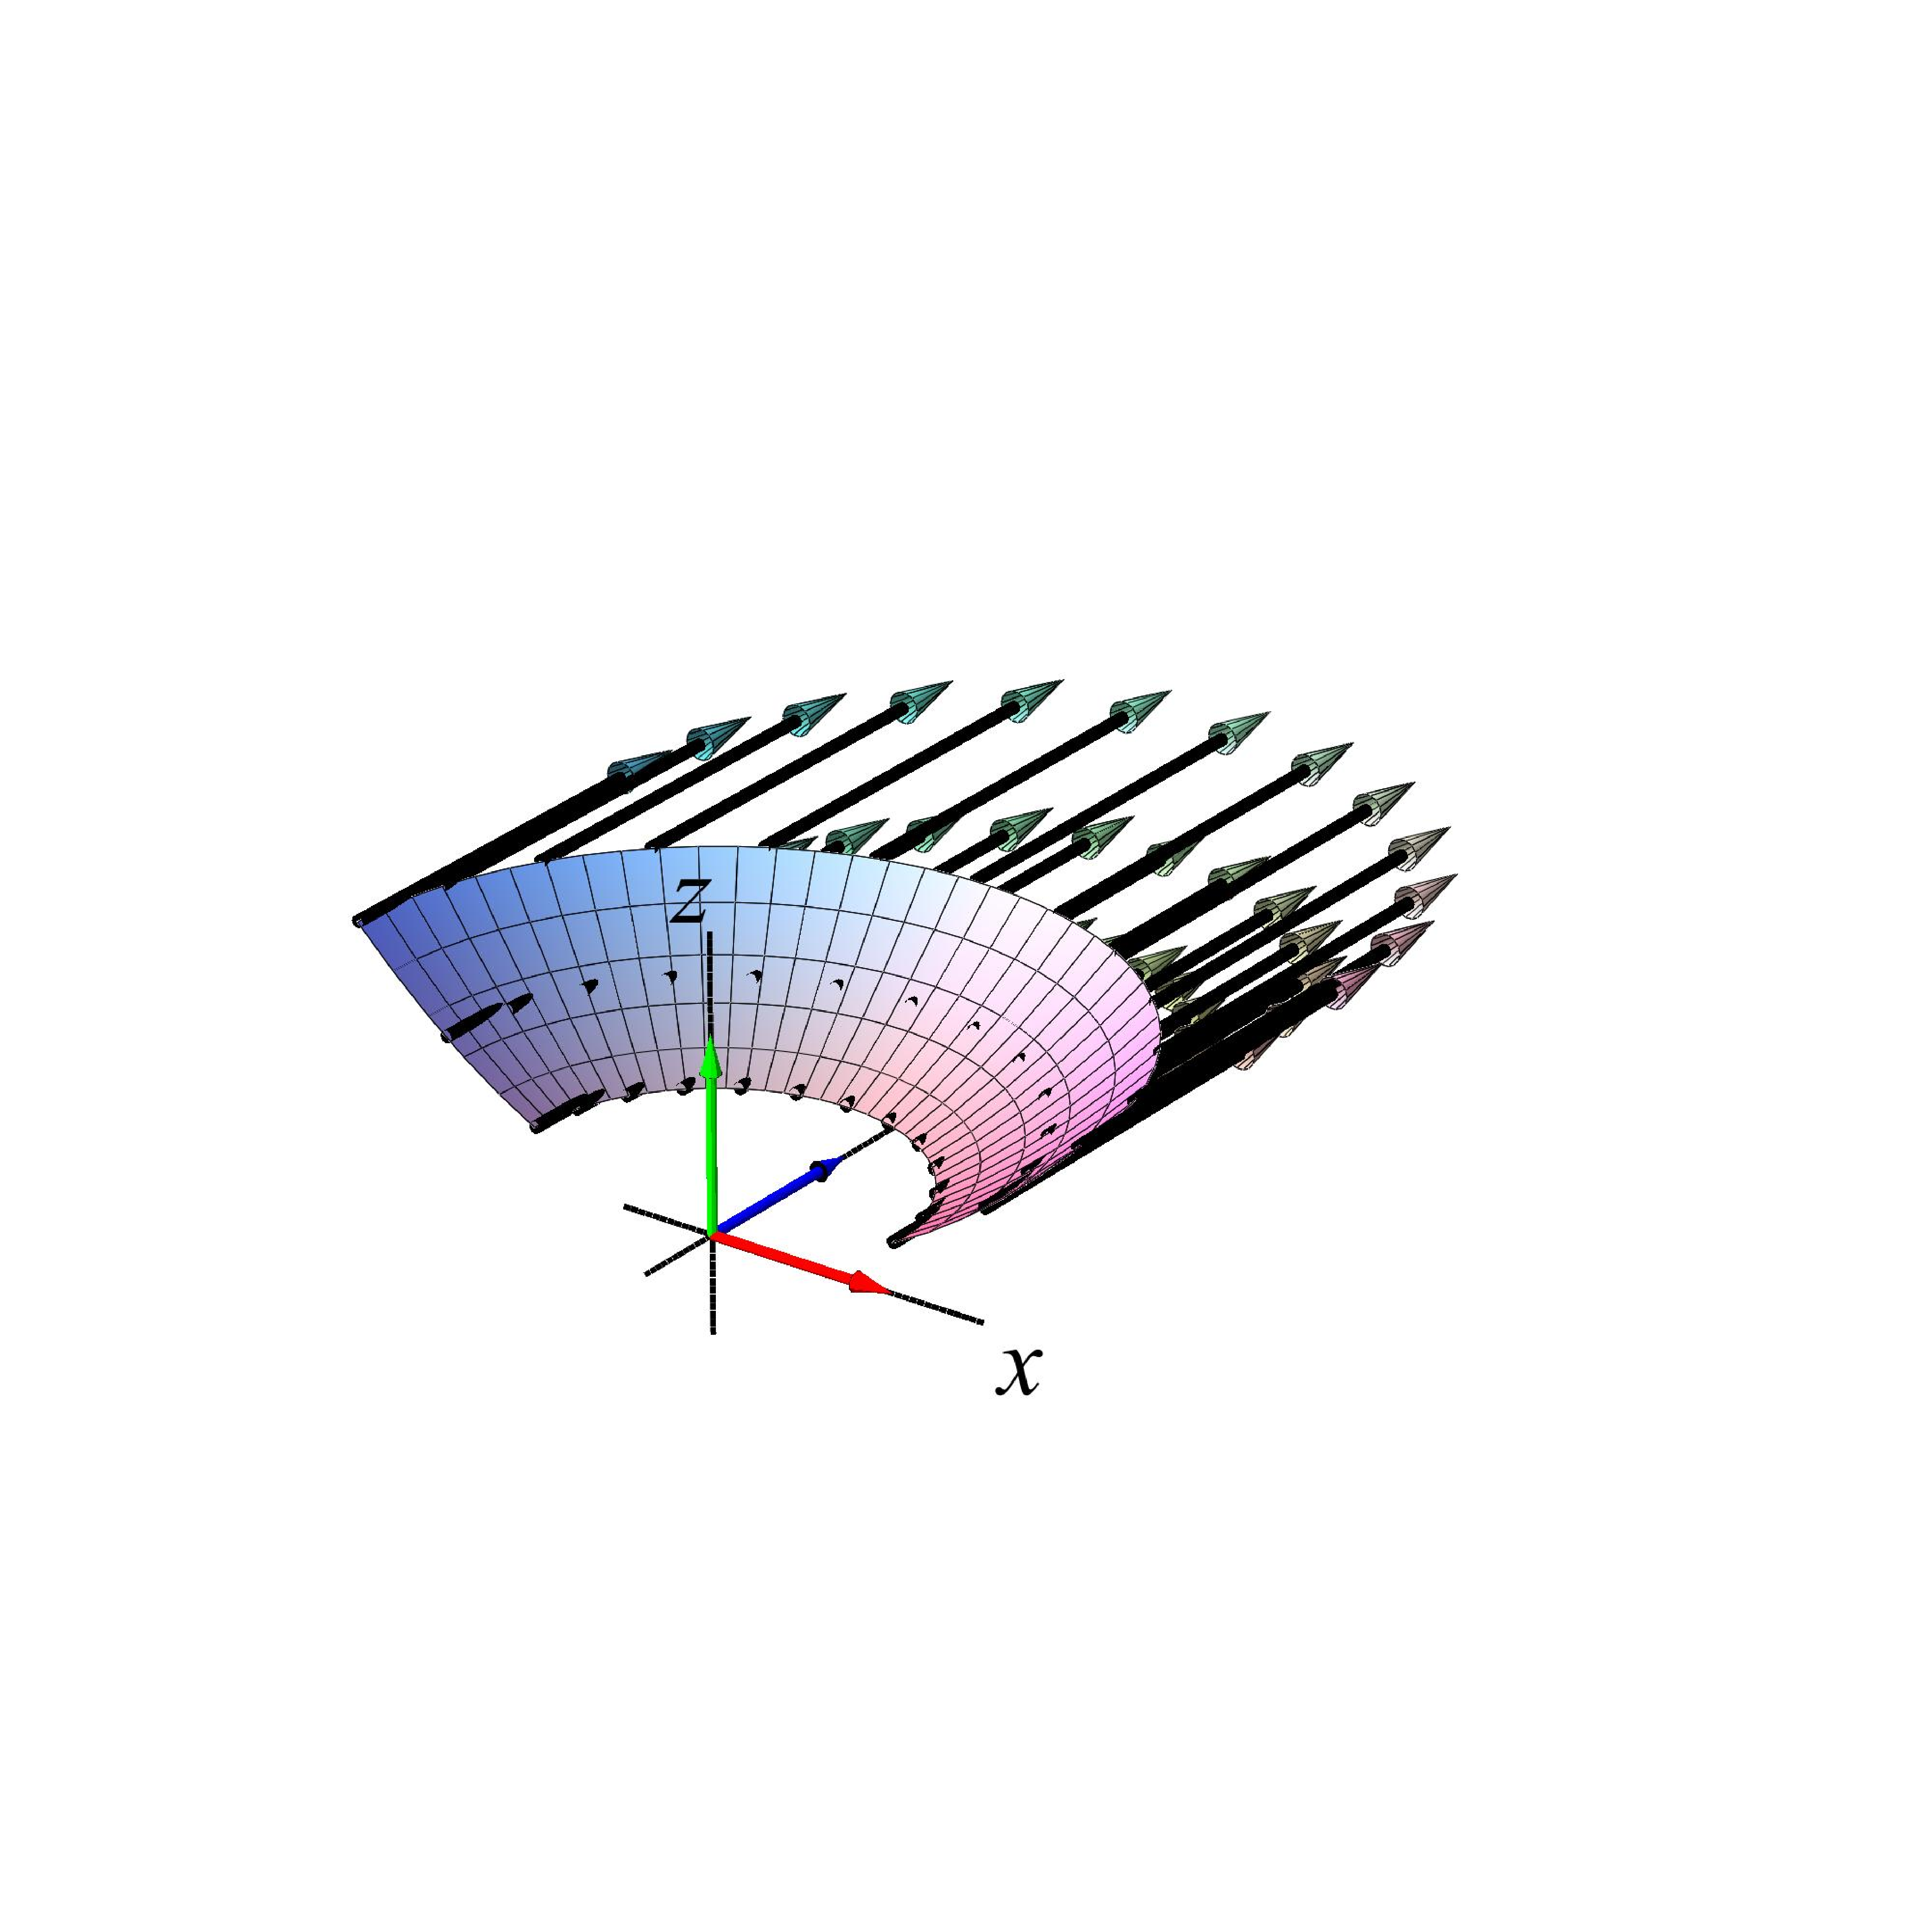
\includegraphics[height=70mm]{FIGS/plotParab4}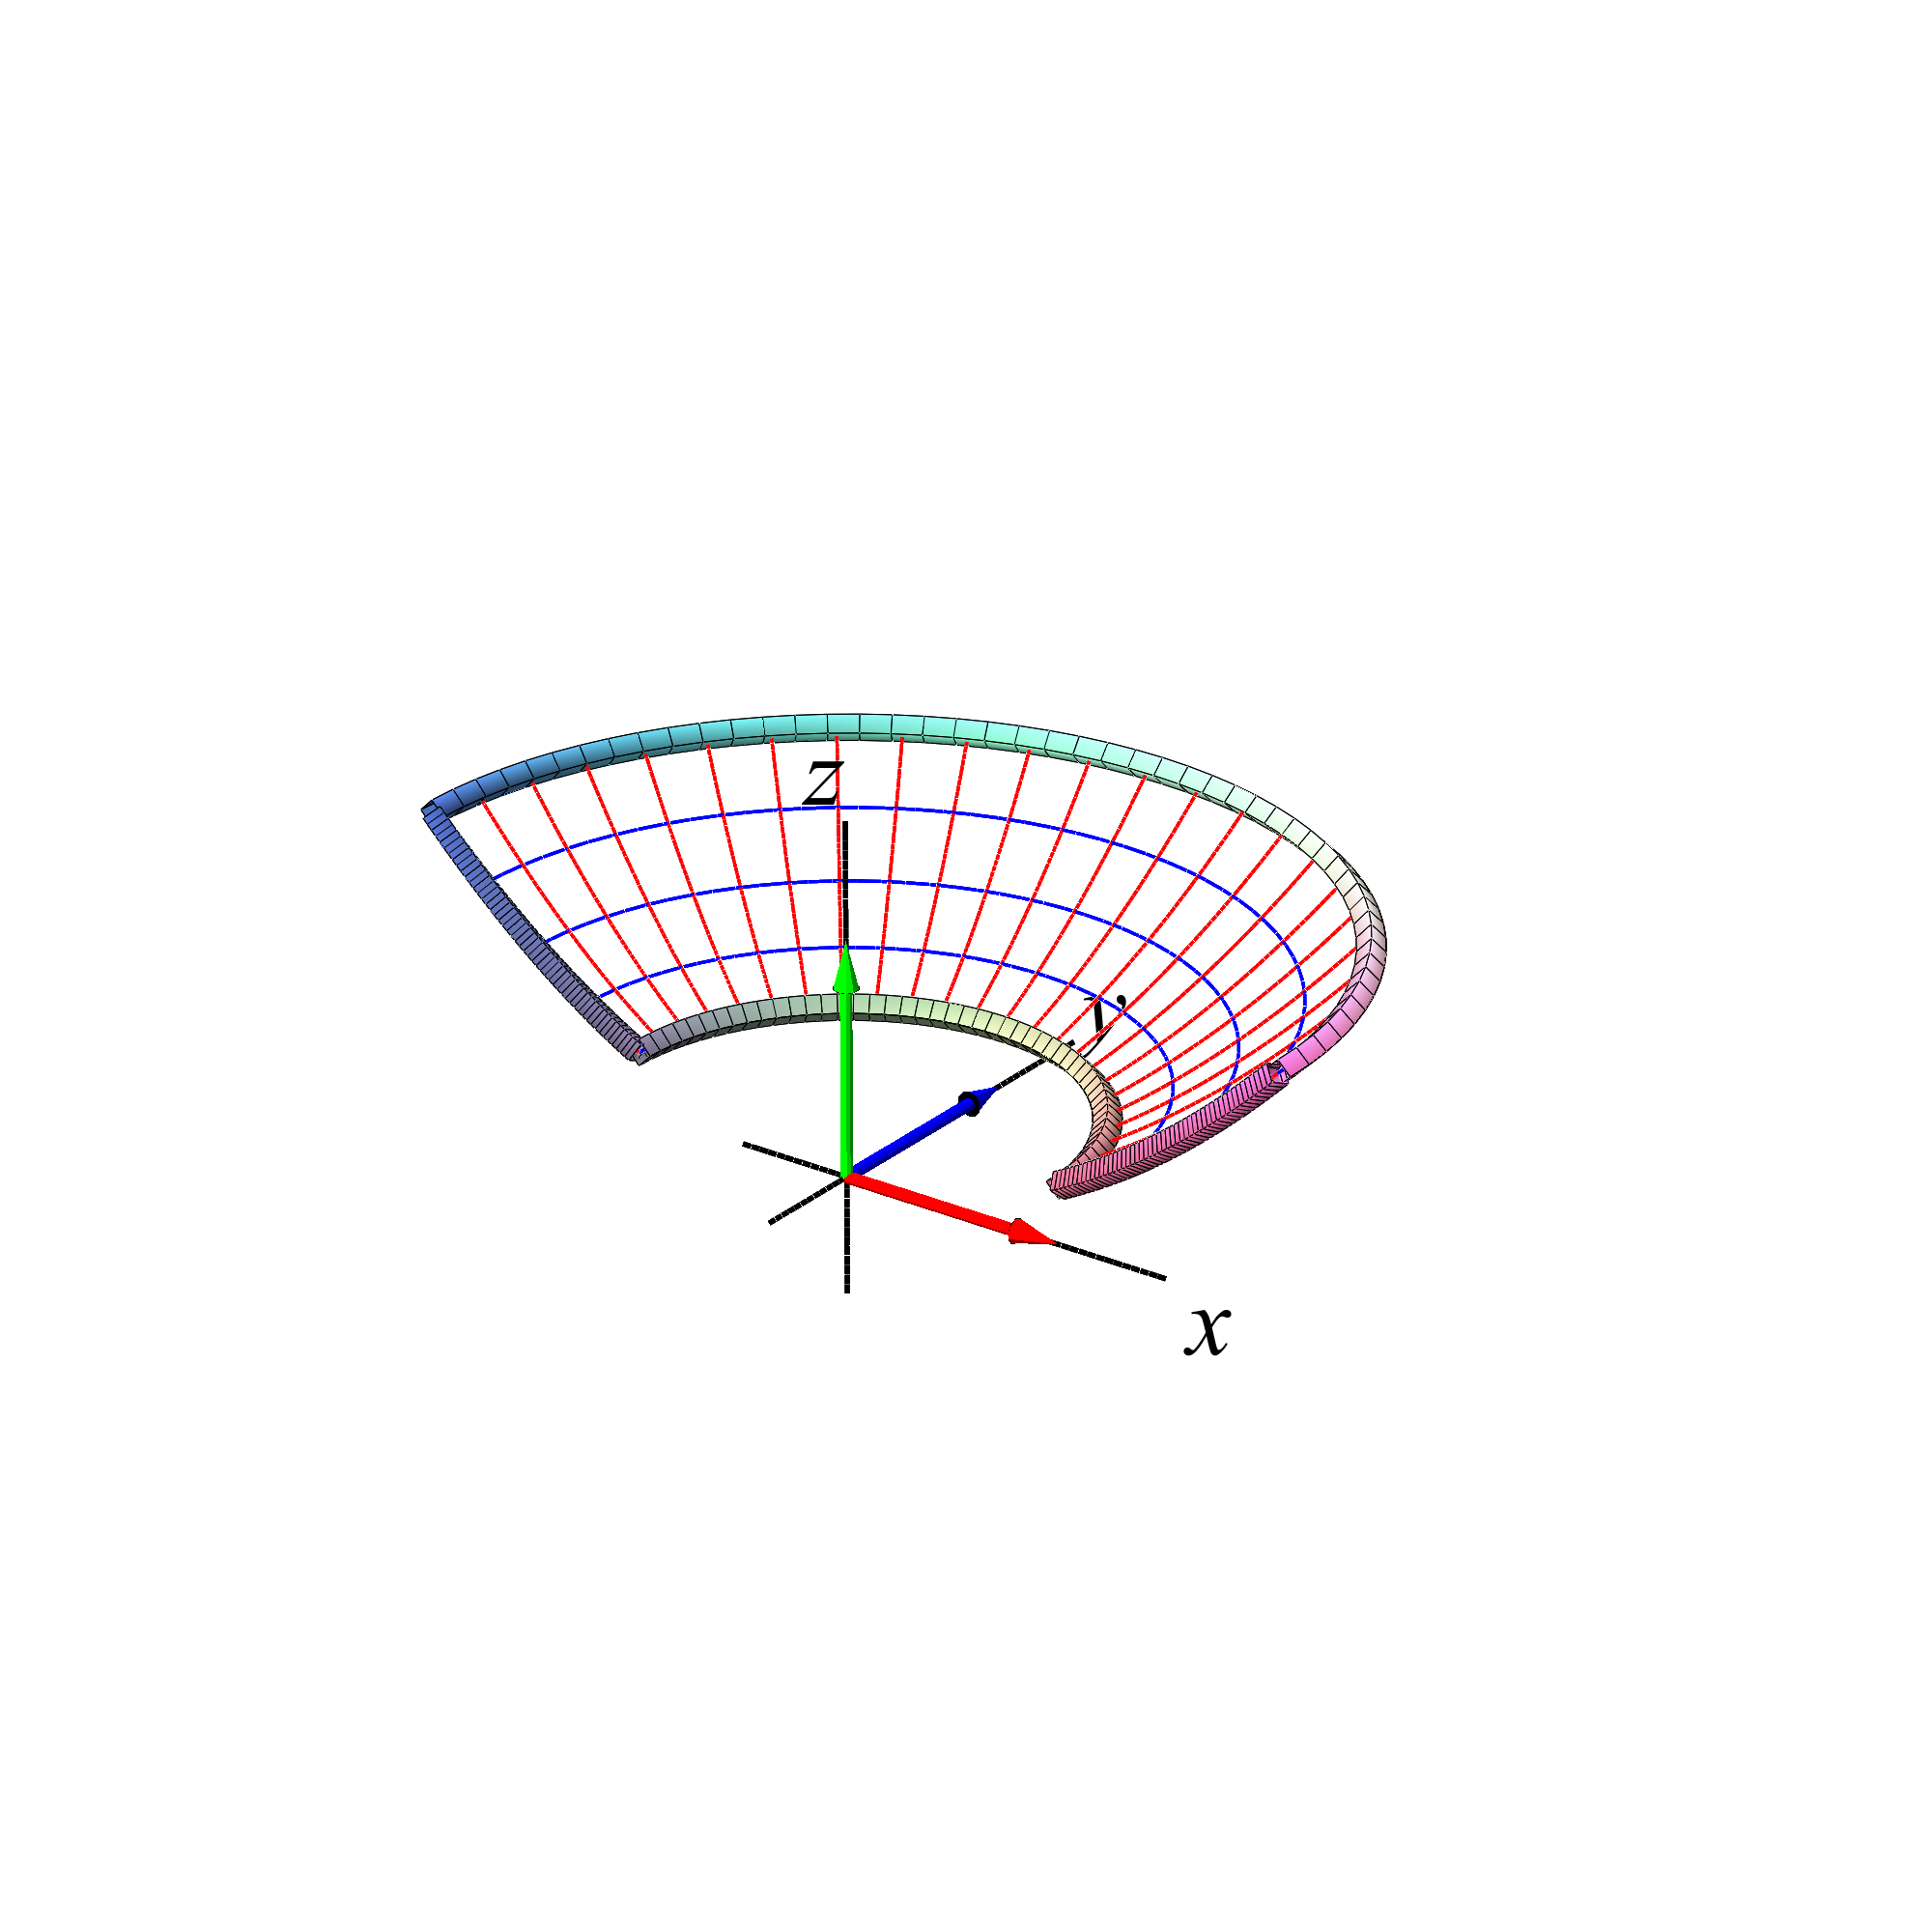
\includegraphics[height=70mm]{FIGS/plotParab5}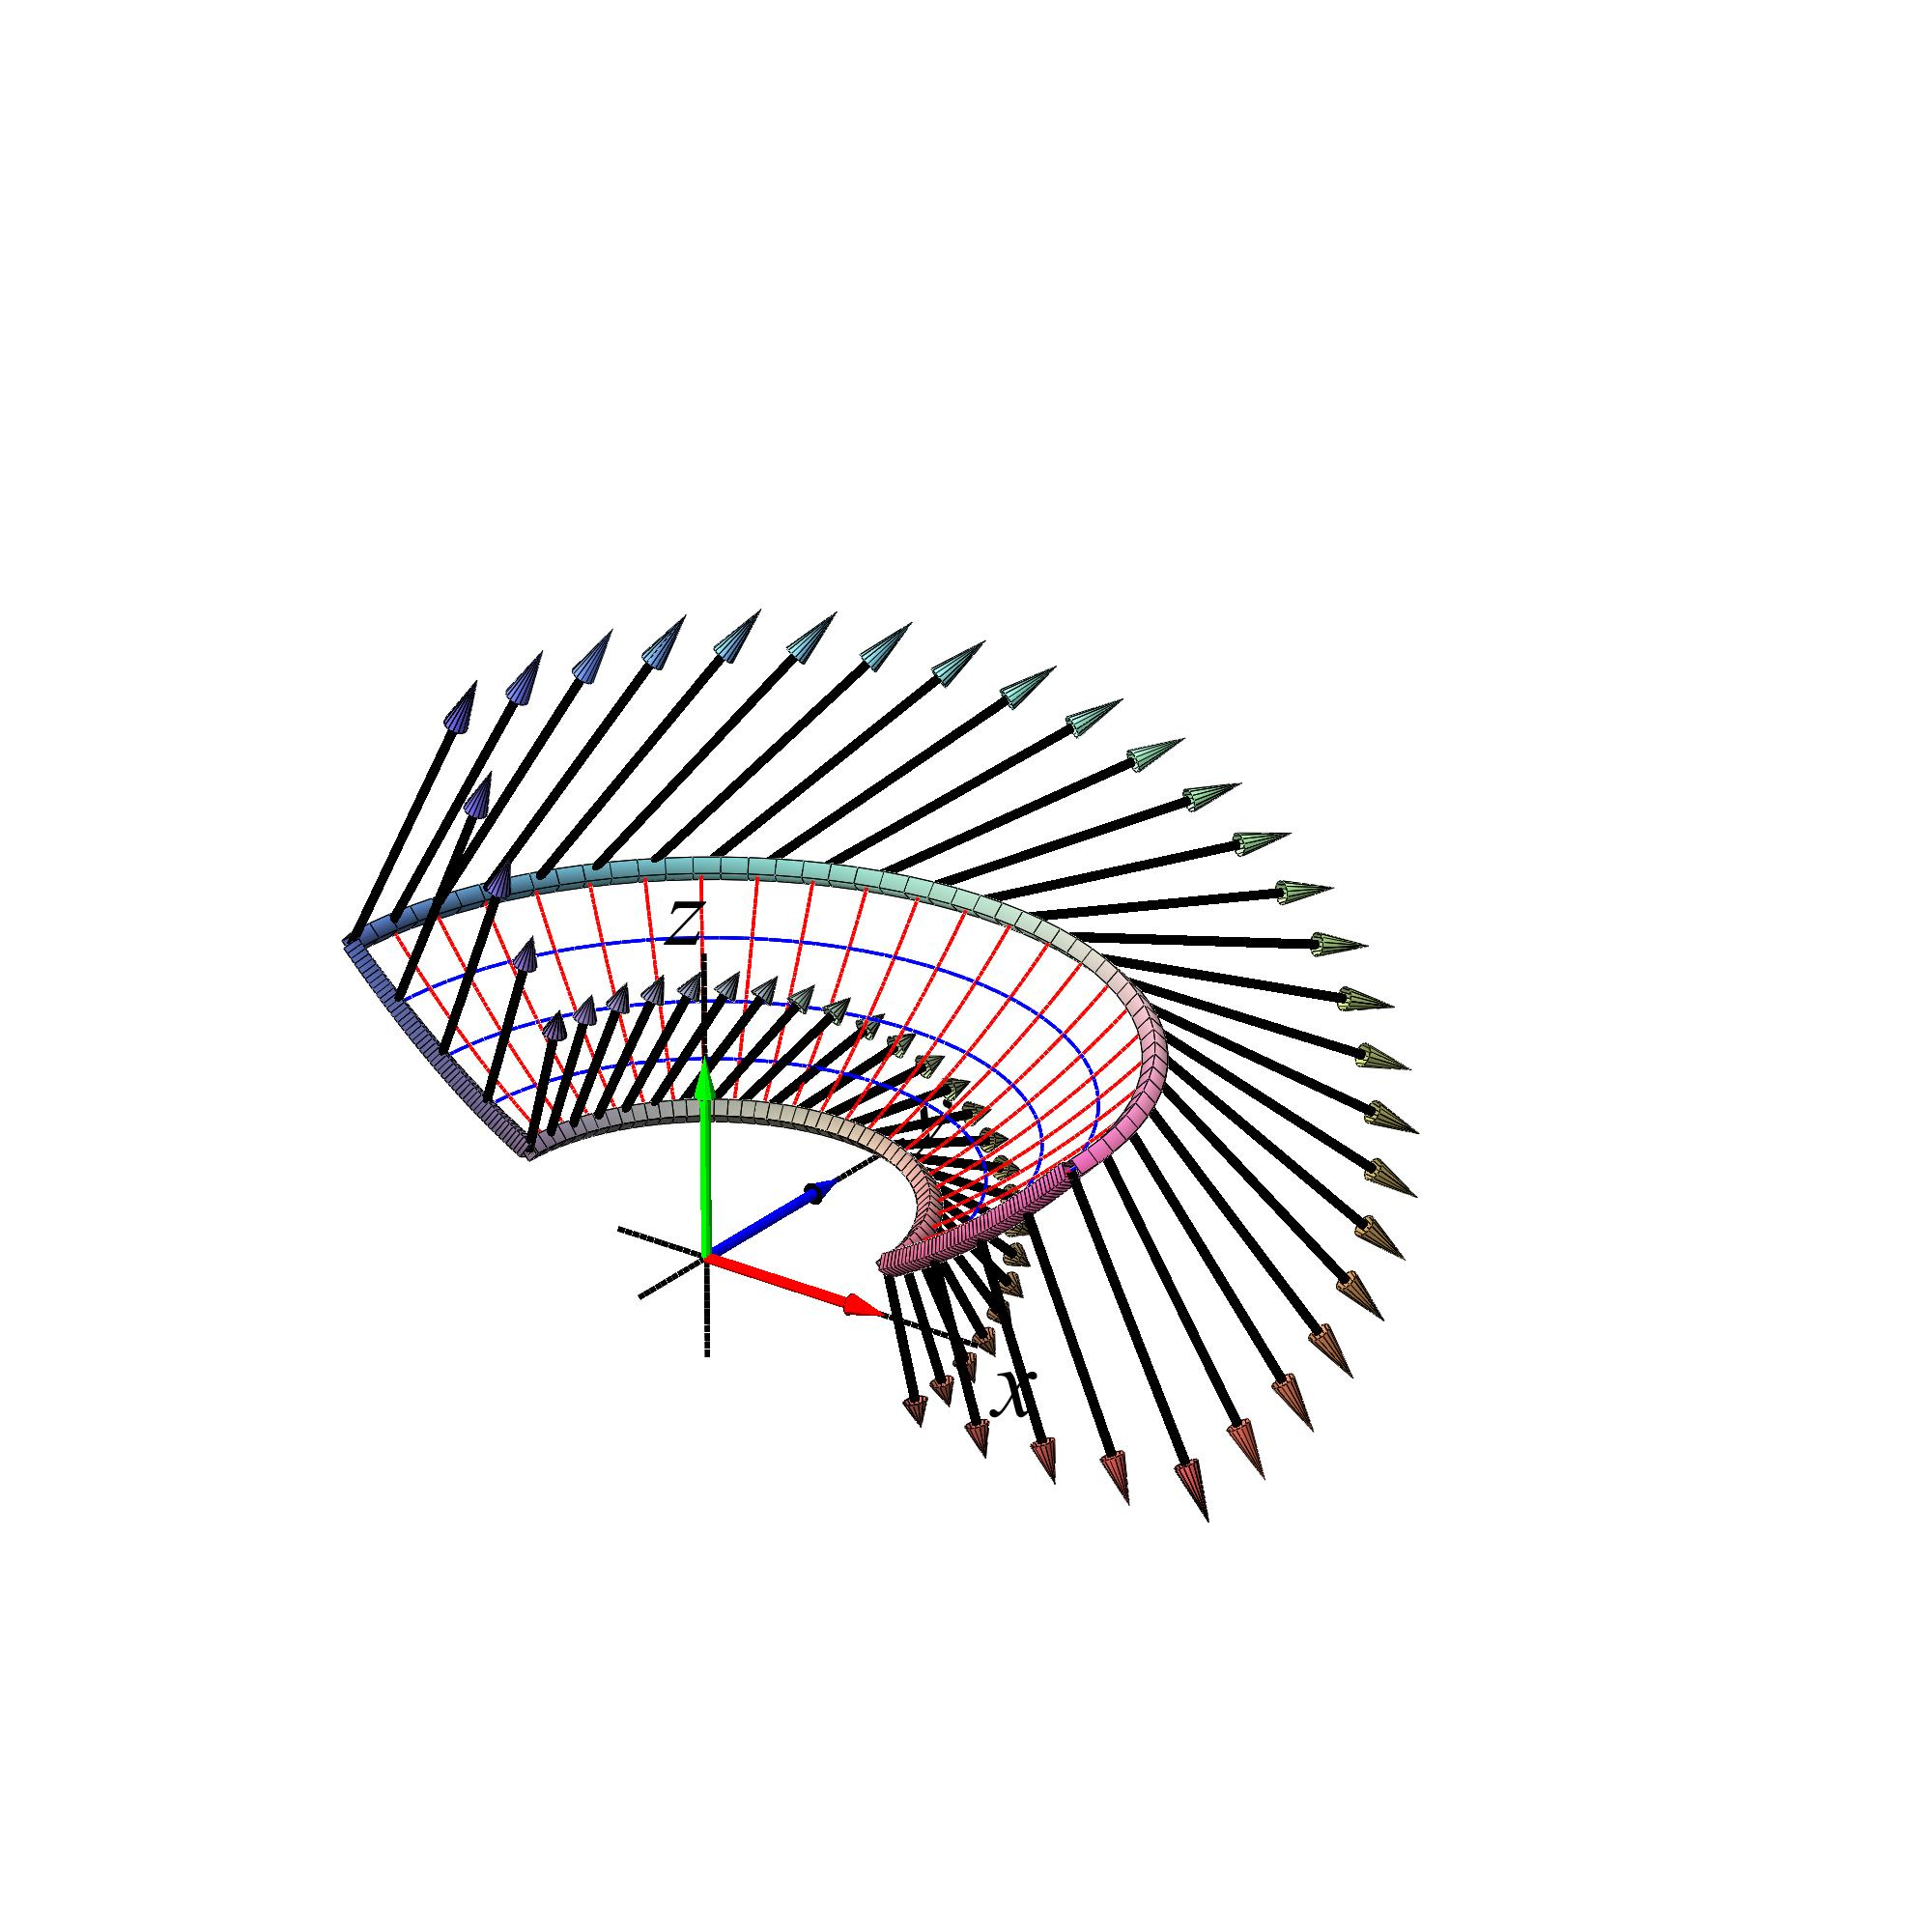
\includegraphics[height=70mm]{FIGS/plotParab6}}
\begin{center}
\caption{\small{Restriktionen af  rotationsvektorfeltet $\Rot(\mathbf{V})(x,y,z)= (0, \, 2, \, 0)$ til et stykke af en paraboloide, fladestykkets rand, og vektorfeltet $\mathbf{V}(x,y,z) = (z, \,y, \, -x)$ restringeret til randen.}}
\label{figParabB}
\end{center}
\end{figure}




%%%%%%%%%%%%%%%%%%%%%%%%%%%%%%%%%%%%%%%%%%%%%%%%%%%%%%%%%%%%%%%%%%%%%%%%%%%%
%%%%%%%%%%%%%%%%%%%%%%%%%%%%%%%%%%%%%%%%%%%%%%%%%%%%%%%%%%%%%%%%%%%%%%%%%%%%
%%%%%%%%%%%%%%%%%%%%%%%%%%%%%%%%%%%%%%%%%%%%%%%%%%%%%%%%%%%%%%%%%%%%%%%%%%%%
%%%%%%%%%%%%%%%%%%%%%%%%%%%%%%%%%%%%%%%%%%%%%%%%%%%%%%%%%%%%%%%%%%%%%%%%%%%%





\begin{exercise}
Lad $F_{\bf{r}}$ betegne den flade, der har
følgende parameterfremstilling og
parameter-område:
\begin{equation}
F_{\bf{r}}\, : \, {\bf{r}}(u,v)\, = \,
((1+u^2)\cos(v),\, (1+u^2)\sin(v),
\,\sin(u))\quad,
\end{equation}
hvor
\begin{equation}
(u,v)
\in [-\frac{\pi}{2},
\,\frac{\pi}{2}]\times[-\pi,\, \frac{\pi}{2}]
\quad .
\end{equation}
Verific\'{e}r at Stokes' sætning er opfyldt for
vektorfeltet ${\bf{V}}\, = \, (yx\,, \,yz\,,
\,xz)$ over fladen $F_{\bf{r}}$ med den givne
rand $\partial F_{\bf{r}}$.
\end{exercise}


\begin{figure}[h]
\centerline{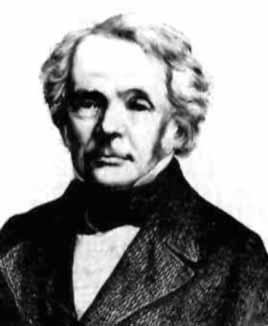
\includegraphics[height=40mm]{FIGS/PERSMobius1790-1868}}
\begin{center}
\caption{\small{August Ferdinand M\"{o}bius, se \href{http://www-history.mcs.st-and.ac.uk/Mathematicians/Mobius.html}{Biografi}.}}
\label{figPERSMob}
\end{center}
\end{figure}




\begin{exercise} \label{exercMob1}
Lad $F_{\bf{r}}$ betegne den flade  -- et såkaldt M\"{o}bius-bånd -- der har
følgende parameterfremstilling og
parameter-område:
\begin{equation}
\begin{aligned}
F_{\bf{r}}\, : \, &{\bf{r}}(u,v)\, \\
&= (2\cos(u)+v\cos(u/2)\cos(u)\, , \,  2\sin(u)+v\cos(u/2)\sin(u)\, , \, v\sin(u/2))
\quad ,
\end{aligned}
\end{equation}
hvor $(u, v) \in [-\pi, \pi] \times [-1, 1]$.
Verific\'{e}r at Stokes' sætning er opfyldt for
vektorfeltet ${\bf{V}}\, = \, (-y\,, \,x\,,
\,1)$ over fladen $F_{\bf{r}}$ med den givne
rand $\partial F_{\bf{r}}$, se Figur \ref{figMob1}: Vis eksplicit, at der
gælder:
\begin{equation} \label{eqMob1}
\int_{F}\, \Rot({\bf{V}})\bm{\cdot} {\bf{n}}_{F} \,
\,d\mu \, = \, \int_{\partial F} \, {\bf{V}}
\bm{\cdot} {\bf{e}}_{\partial F} \, d\mu \, = \, -32 \quad .
\end{equation}
\end{exercise}

\begin{figure}[h]
\centerline{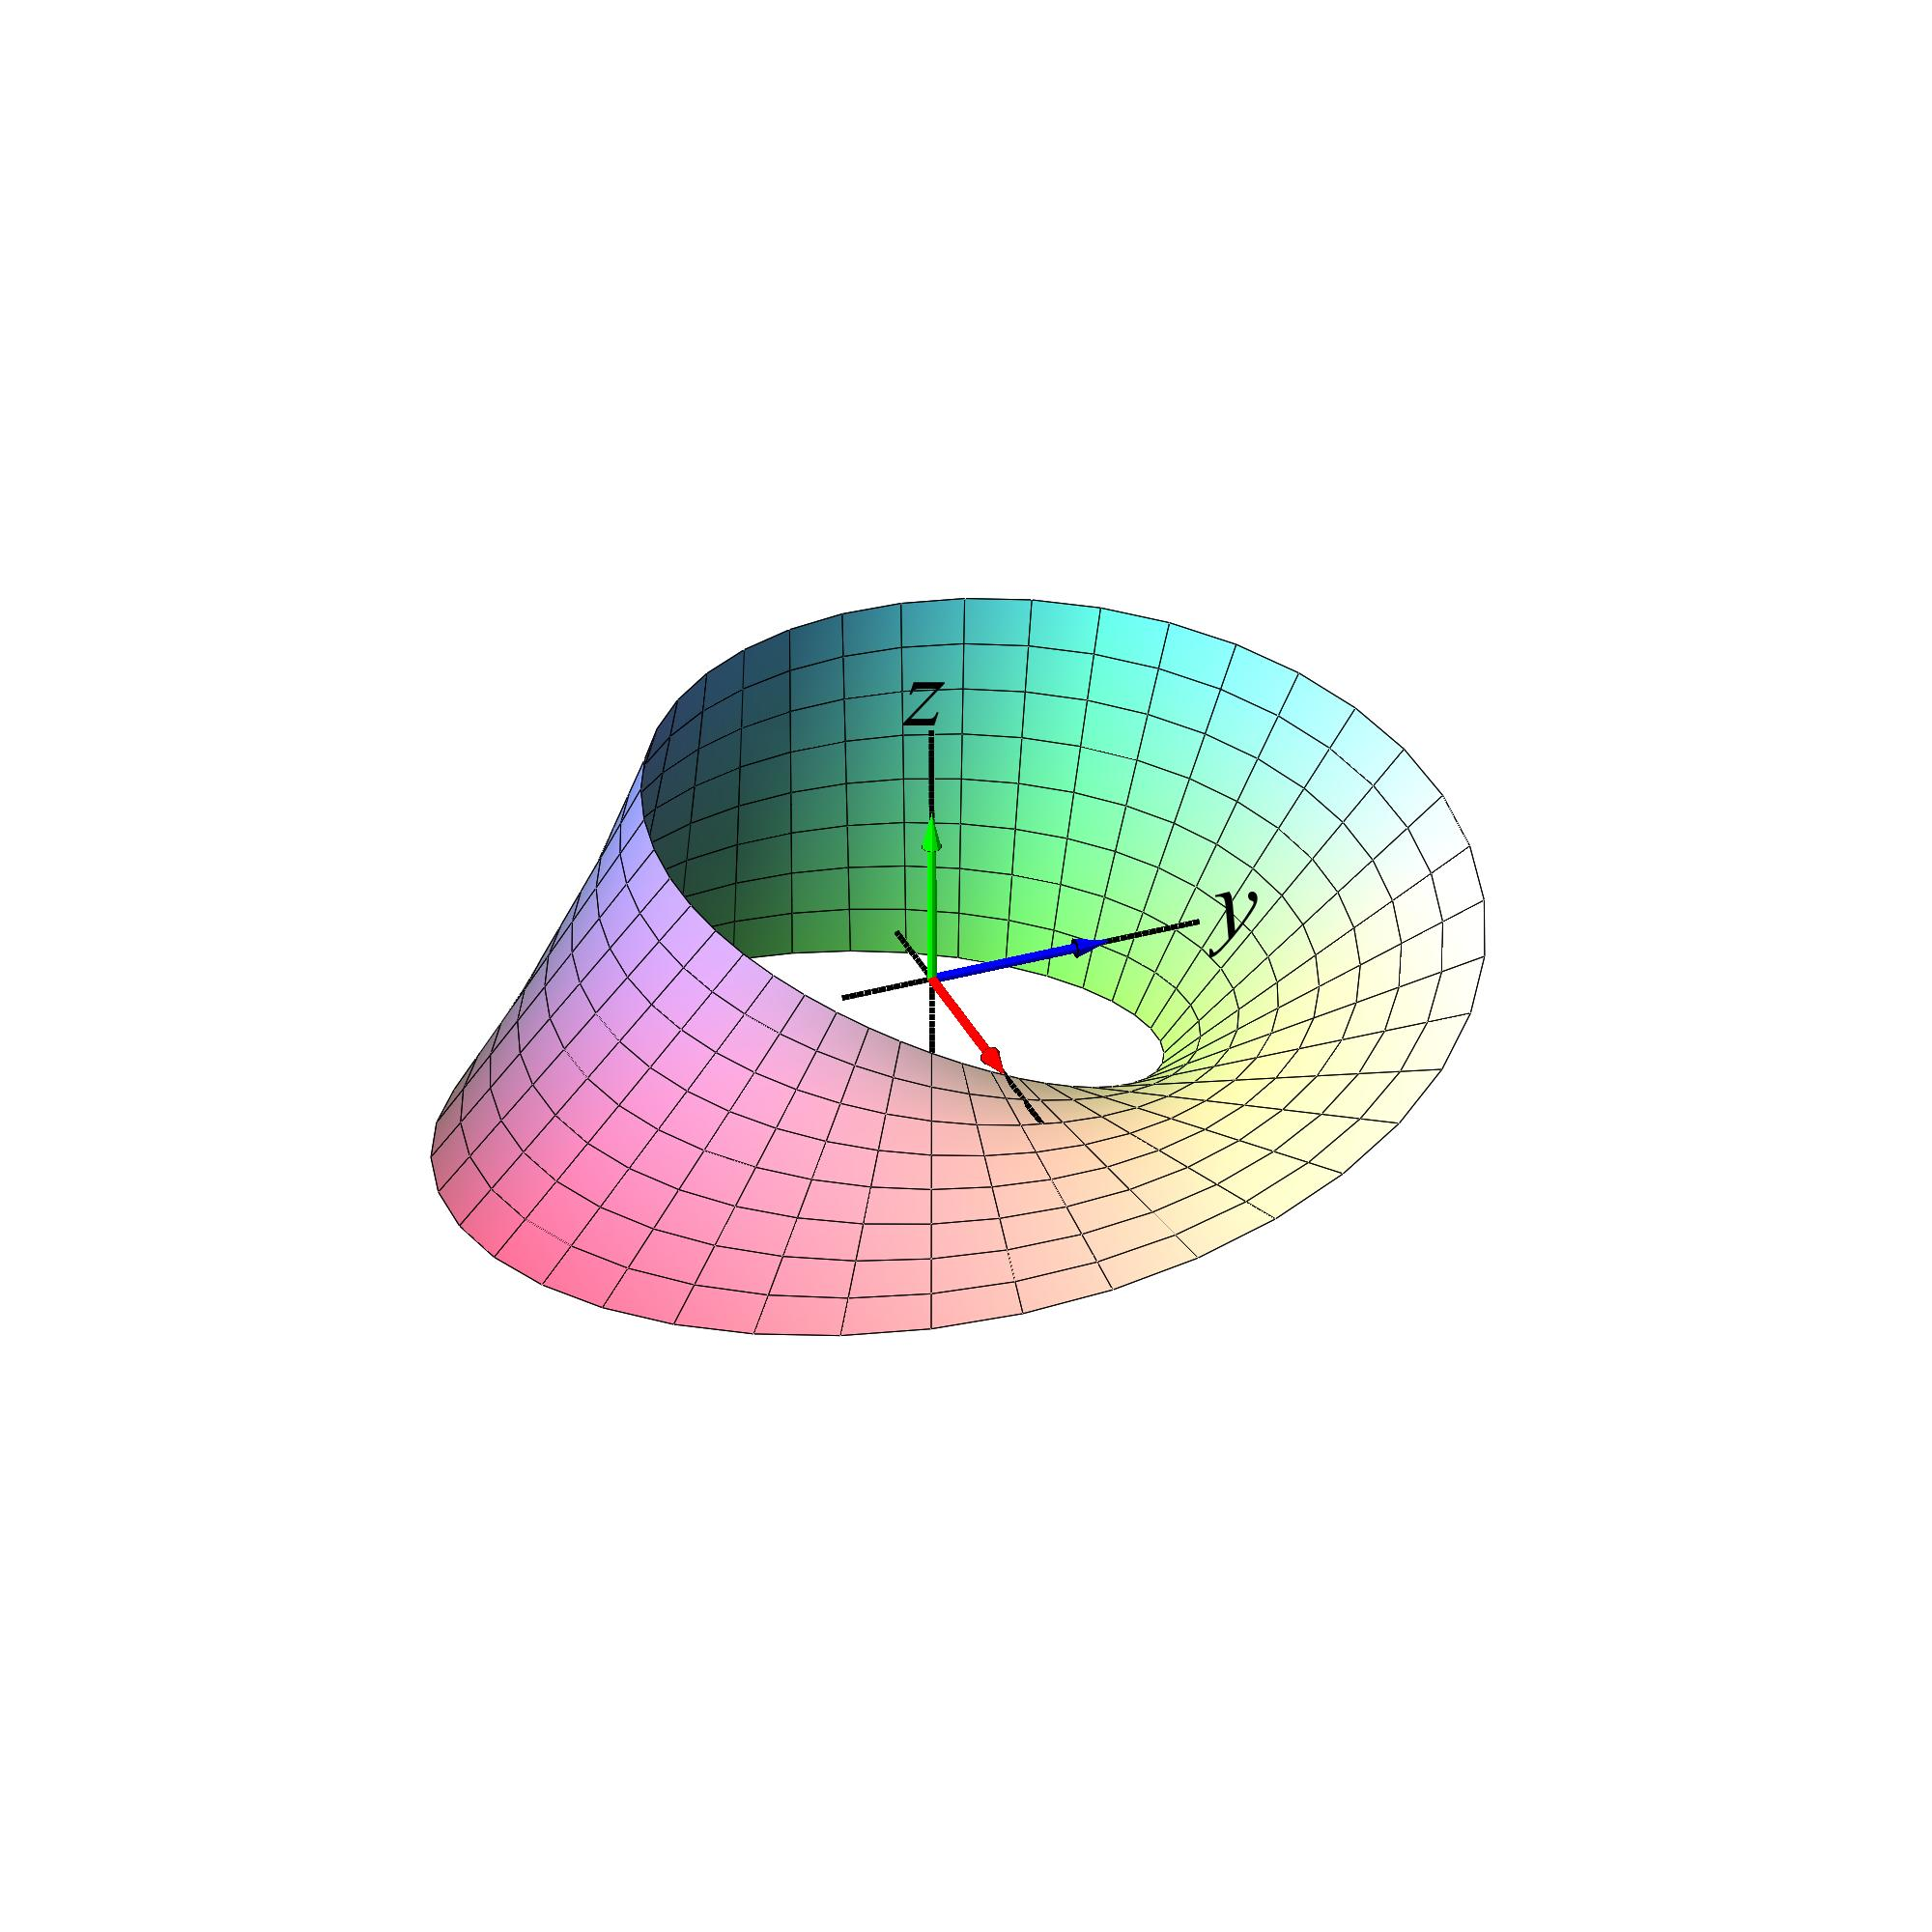
\includegraphics[height=70mm]{FIGS/plotMobius1}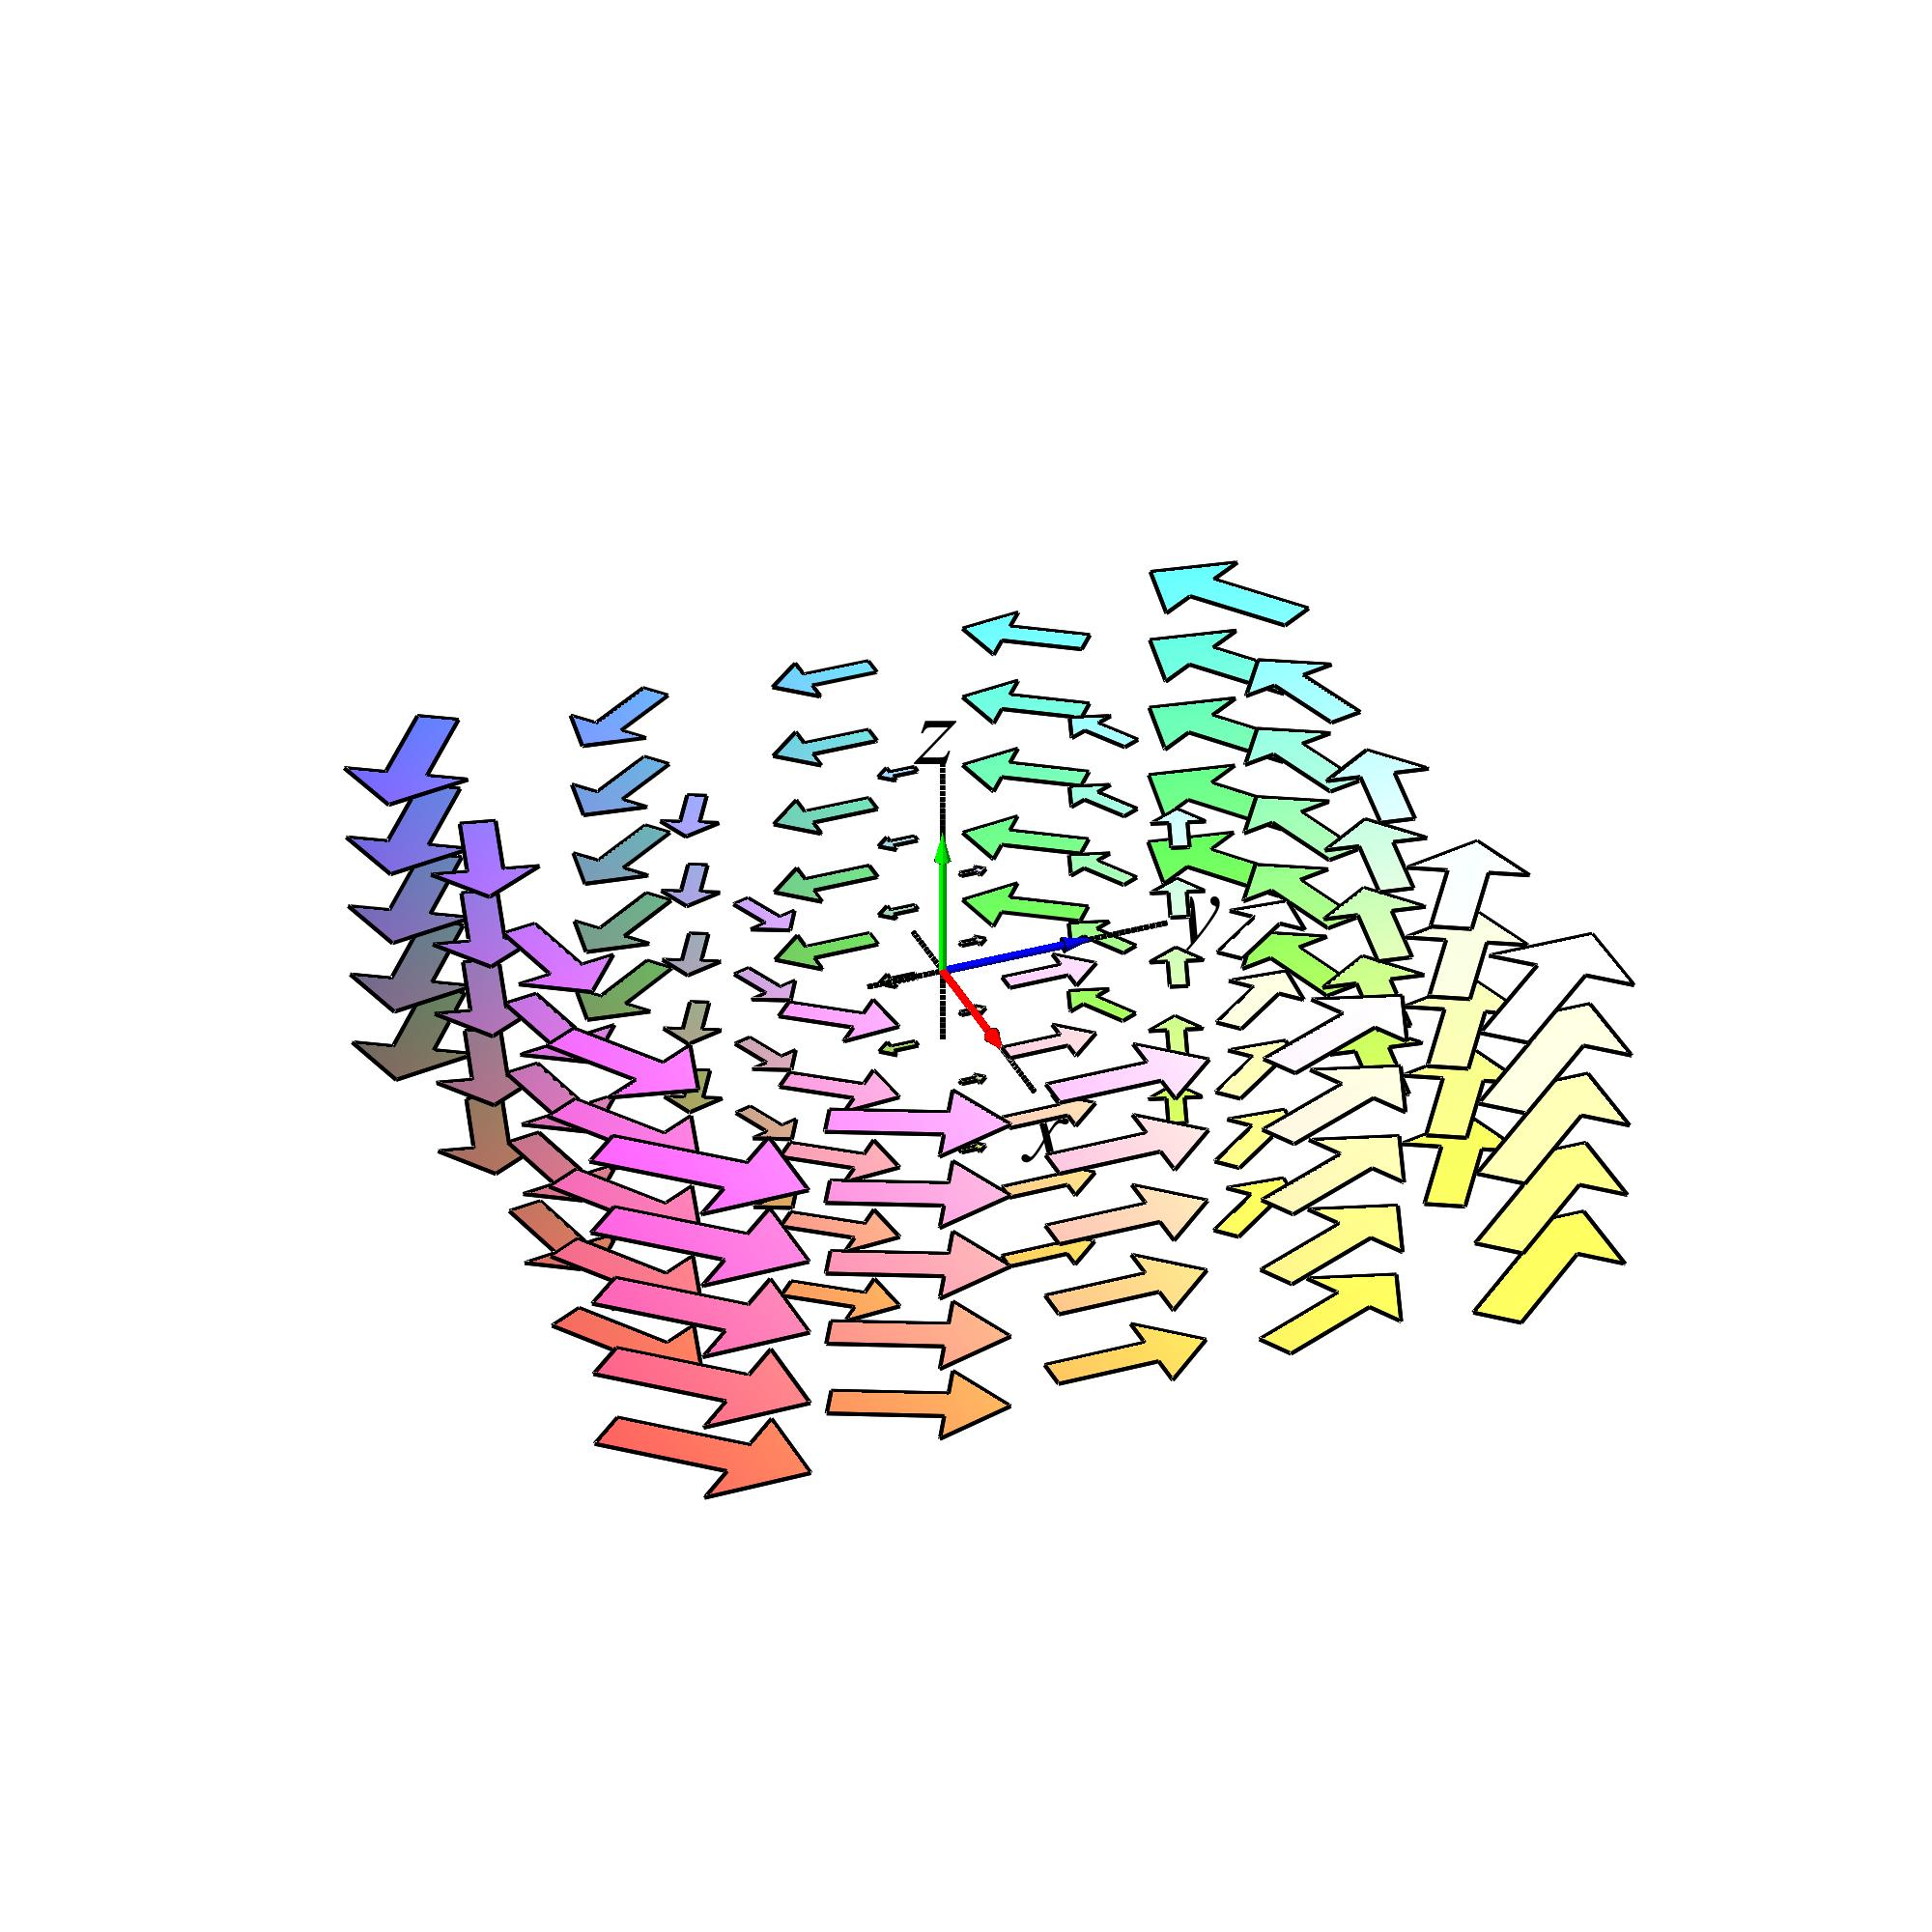
\includegraphics[height=70mm]{FIGS/plotMobius2}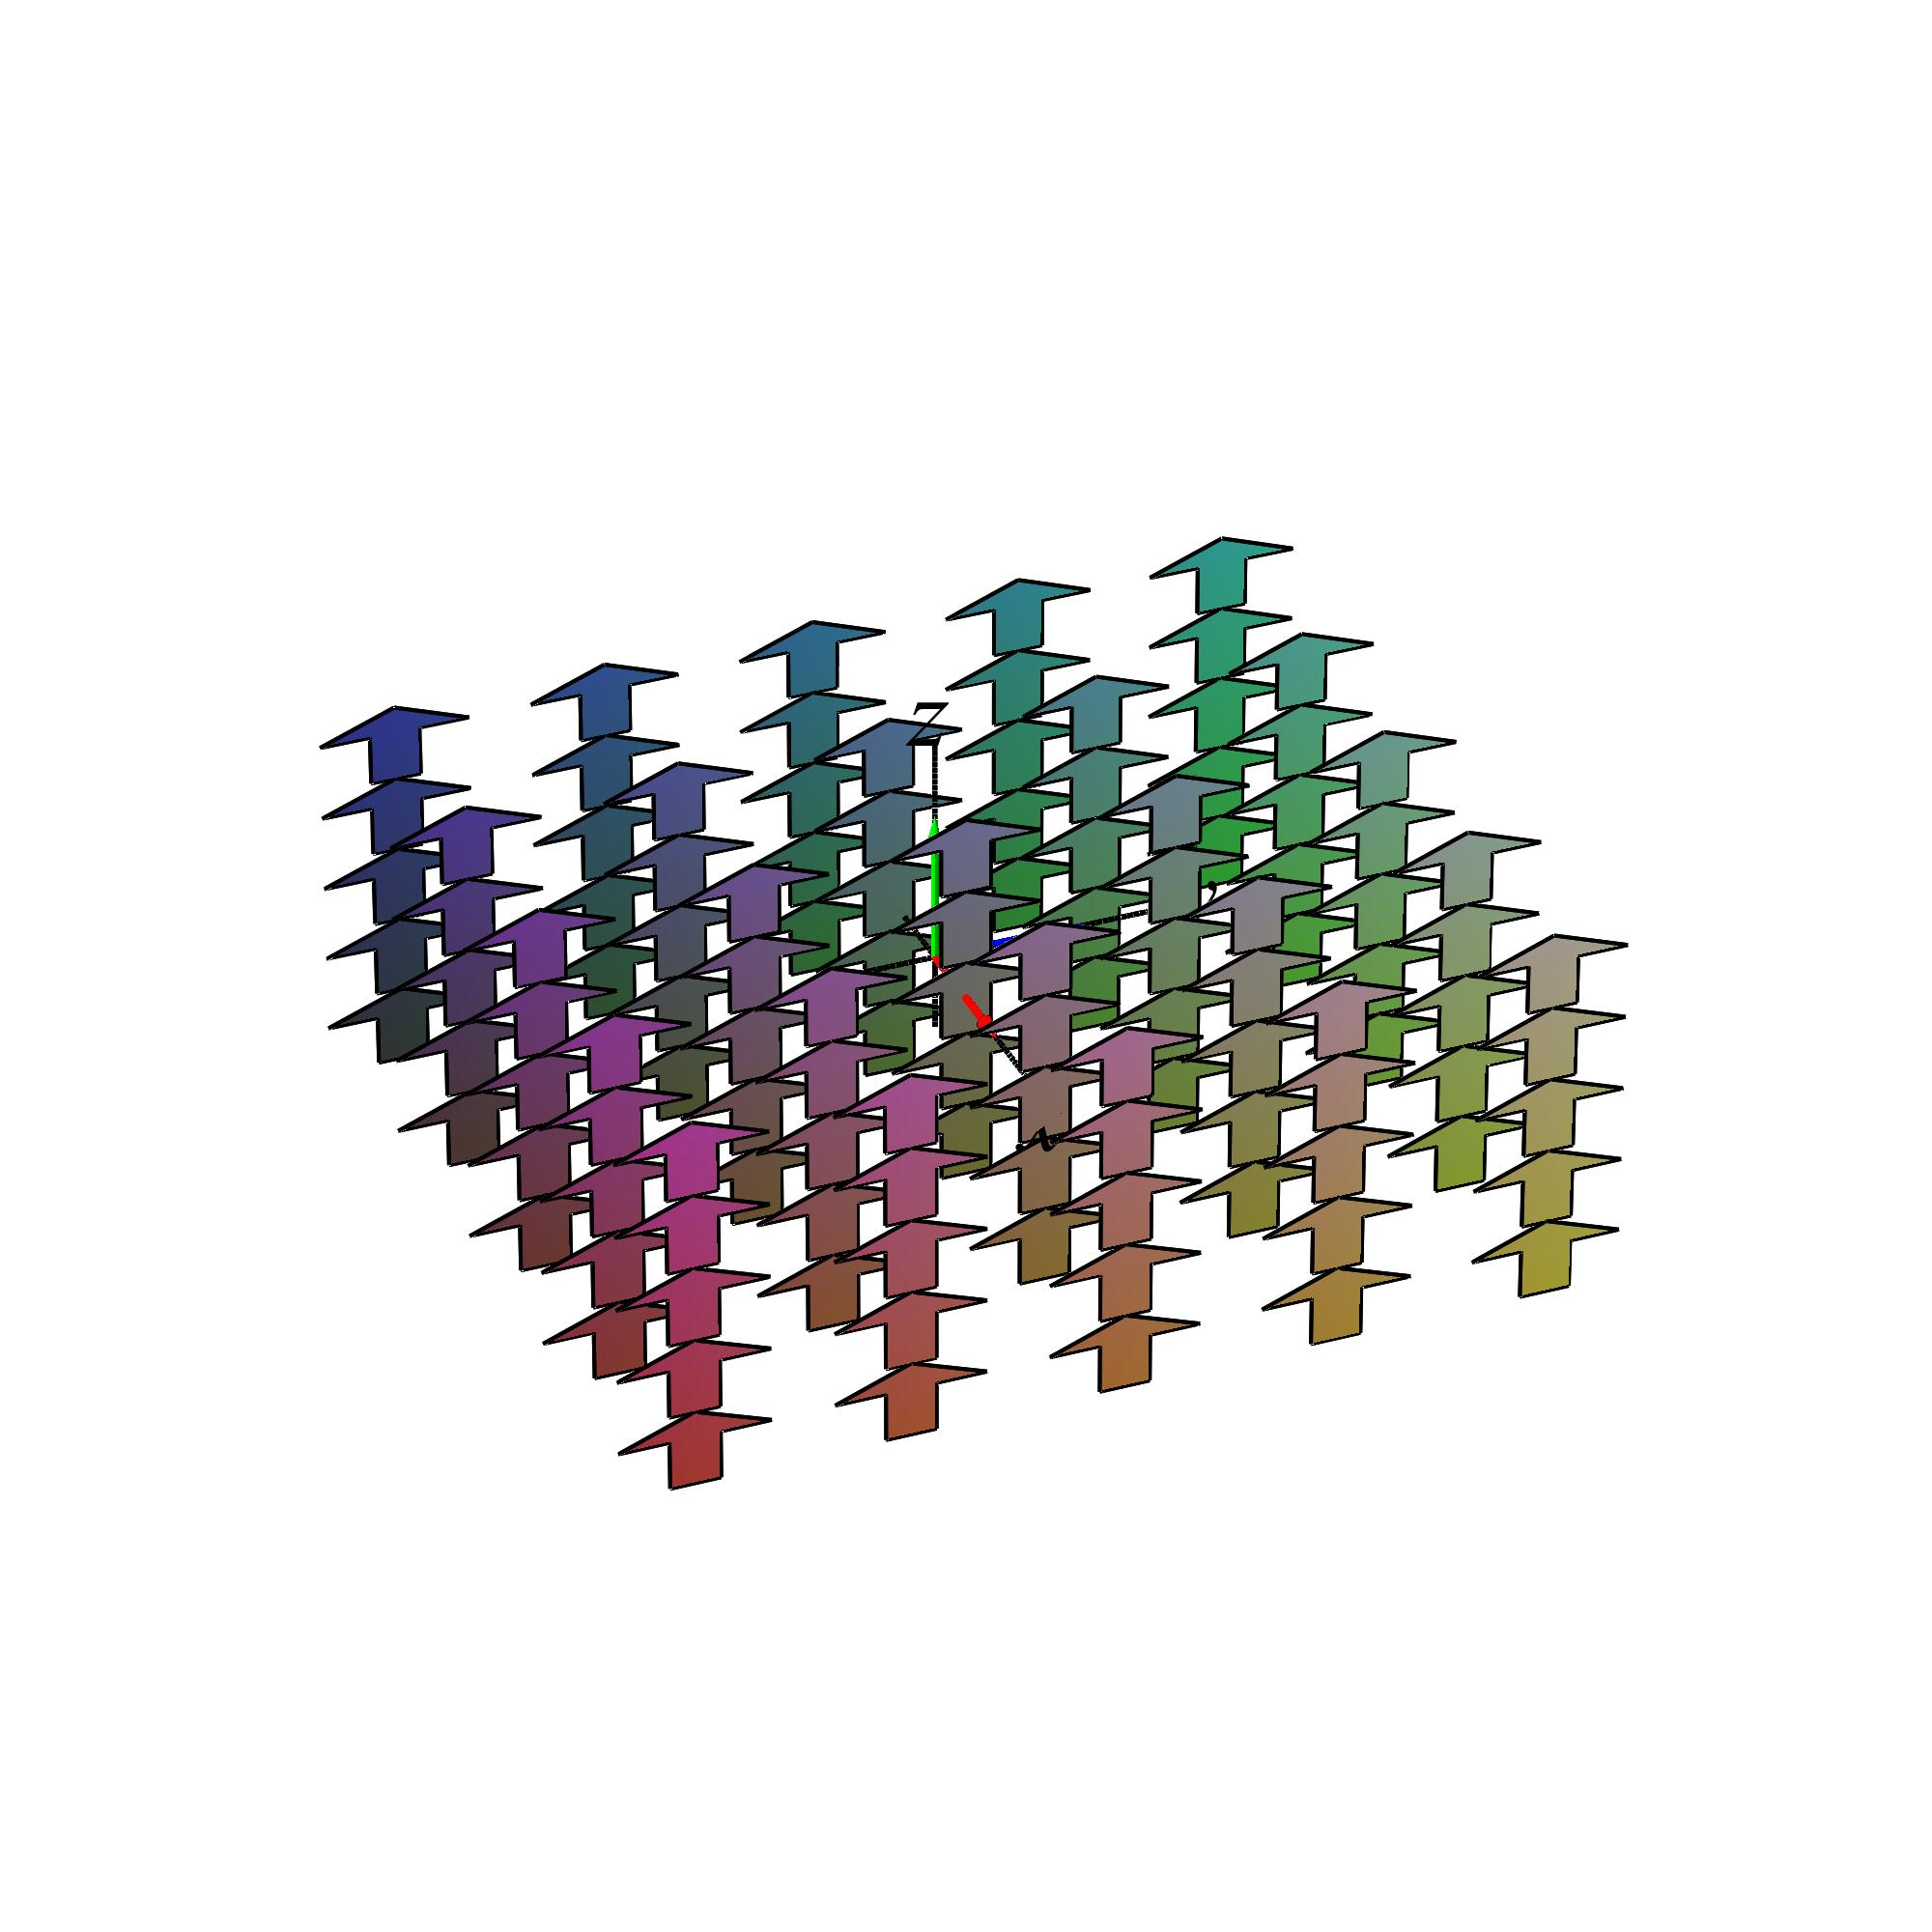
\includegraphics[height=70mm]{FIGS/plotMobius3}}
\begin{center}
\caption{\small{Et M\"{o}bius bånd i et vektorfelt $\mathbf{V}(x,y,z) = (-y, x, 1)$ (i midten) og  vektorfeltets rotationsvektorfelt  $\Rot(\mathbf{V})(x,y,z)= (0,0,2)$.}}
\label{figMob1}
\end{center}
\end{figure}


\begin{exercise} \label{exercMob2}
Lad nu $G_{\bf{r}}$ betegne det samme Møbius-bånd som  i opgave \ref{exercMob1}:
\begin{equation}
\begin{aligned}
G_{\bf{r}}\, : \, &{\bf{r}}(u,v)\, \\
&=
(2\cos(u)+v\cos(u/2)\cos(u)\, , \,  2\sin(u)+v\cos(u/2)\sin(u)\, , \, v\sin(u/2)) \quad ,
\end{aligned}
\end{equation}
men nu med et lidt modificeret parameterområde:
\begin{equation}
(u, v) \in [0, 2\pi] \times [-1, 1] \quad .
\end{equation}
Verific\'{e}r at Stokes' sætning er opfyldt for
vektorfeltet ${\bf{V}}\, = \, (-y\,, \,x\,,
\,1)$ over fladen $G_{\bf{r}}$ med den givne
rand $\partial G_{\bf{r}}$: Vis eksplicit, at der
gælder:
\begin{equation} \label{eqMob2}
\int_{G_{\mathbf{r}}}\, \Rot({\bf{V}})\bm{\cdot} {\bf{n}}_{G} \,
\,d\mu \, = \, \int_{\partial G_{\mathbf{r}}} \, {\bf{V}}
\bm{\cdot} {\bf{e}}_{\partial G} \, d\mu \, = \, 0 \quad .
\end{equation}
\end{exercise}



\begin{exercise} \label{exercMob3}
Forklar forskellen mellem de to (værdi-)resultater (henholdsvis $-32$ og $0$), der opnås i henholdsvis
(\ref{eqMob1}) og (\ref{eqMob2}). Vink: Hold øje med normalvektorfeltet $\mathbf{n}_{F}$. \\

Hvilke \emph{værdier} for rotationsflux og cirkulation opnås ved at
skifte intervaller i parametriseringen, dvs. ved blot at benytte følgende parameterintervaller for forskellige $\alpha \in \mathbb{R}$:
\begin{equation}
(u, v) \in [-\pi + \alpha, \pi + \alpha] \times [-1, 1] \quad ?
\end{equation}
\end{exercise}

\begin{figure}[h]
\centerline{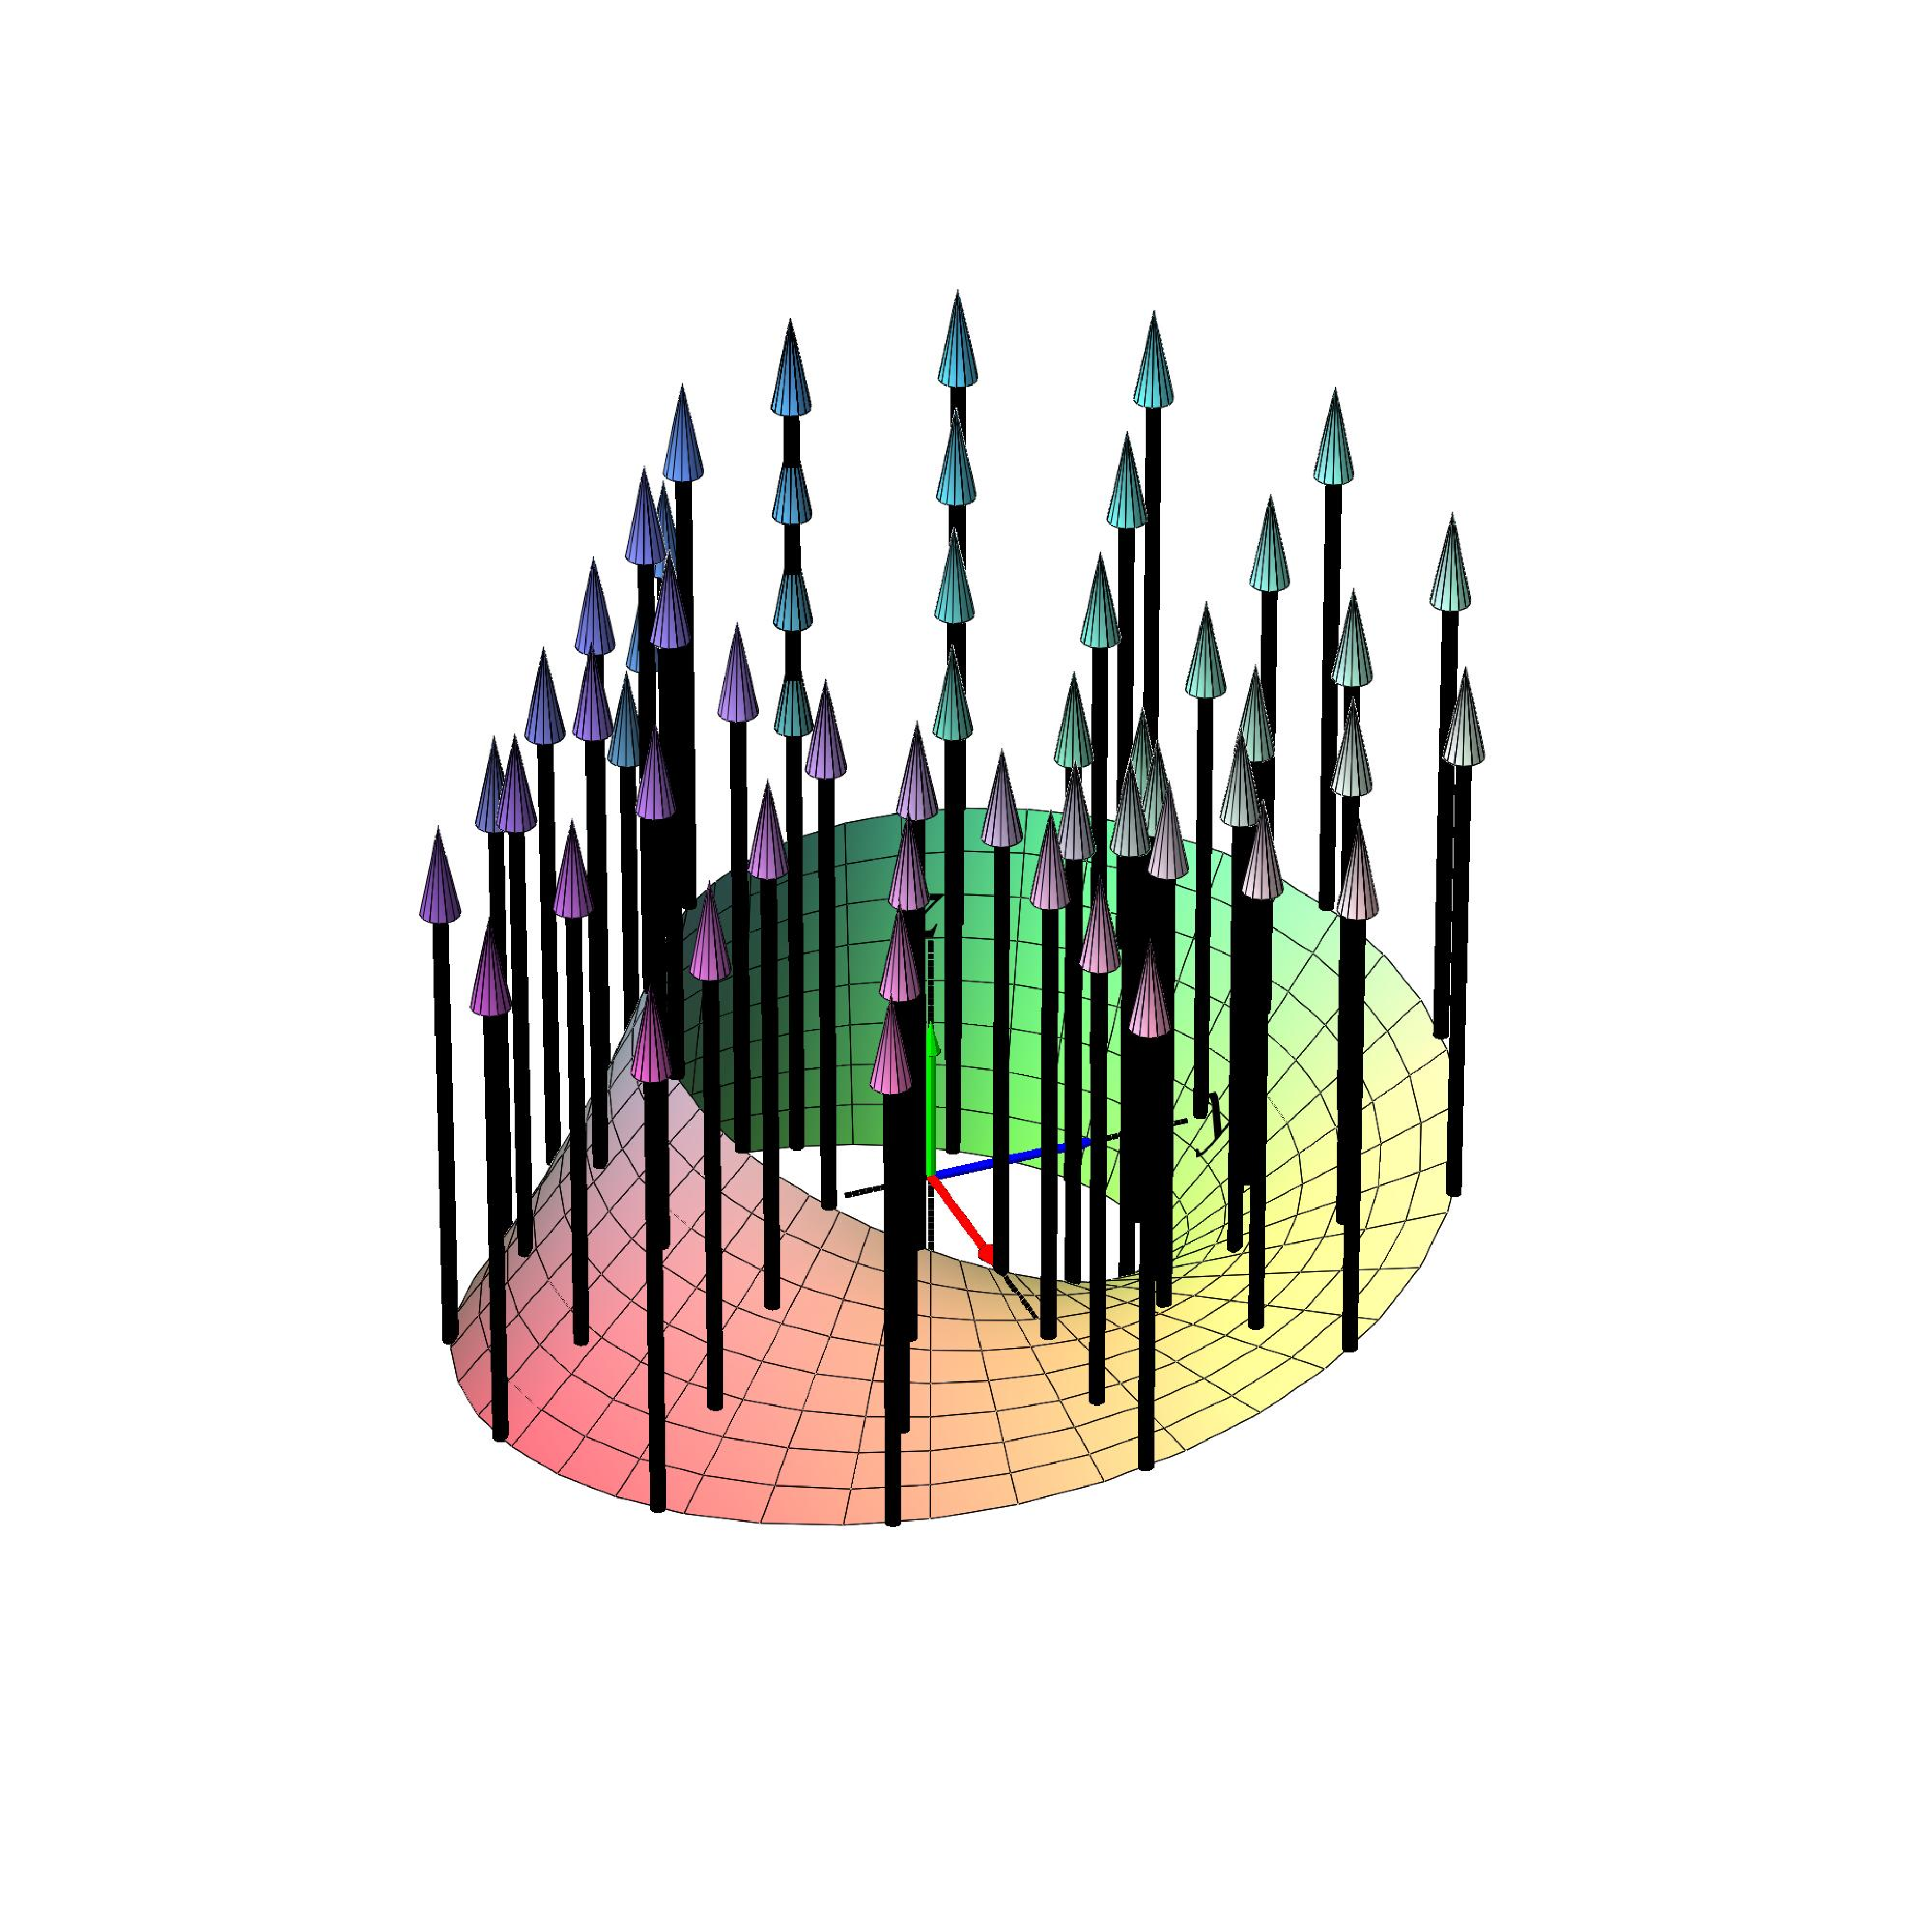
\includegraphics[height=70mm]{FIGS/plotMobius4}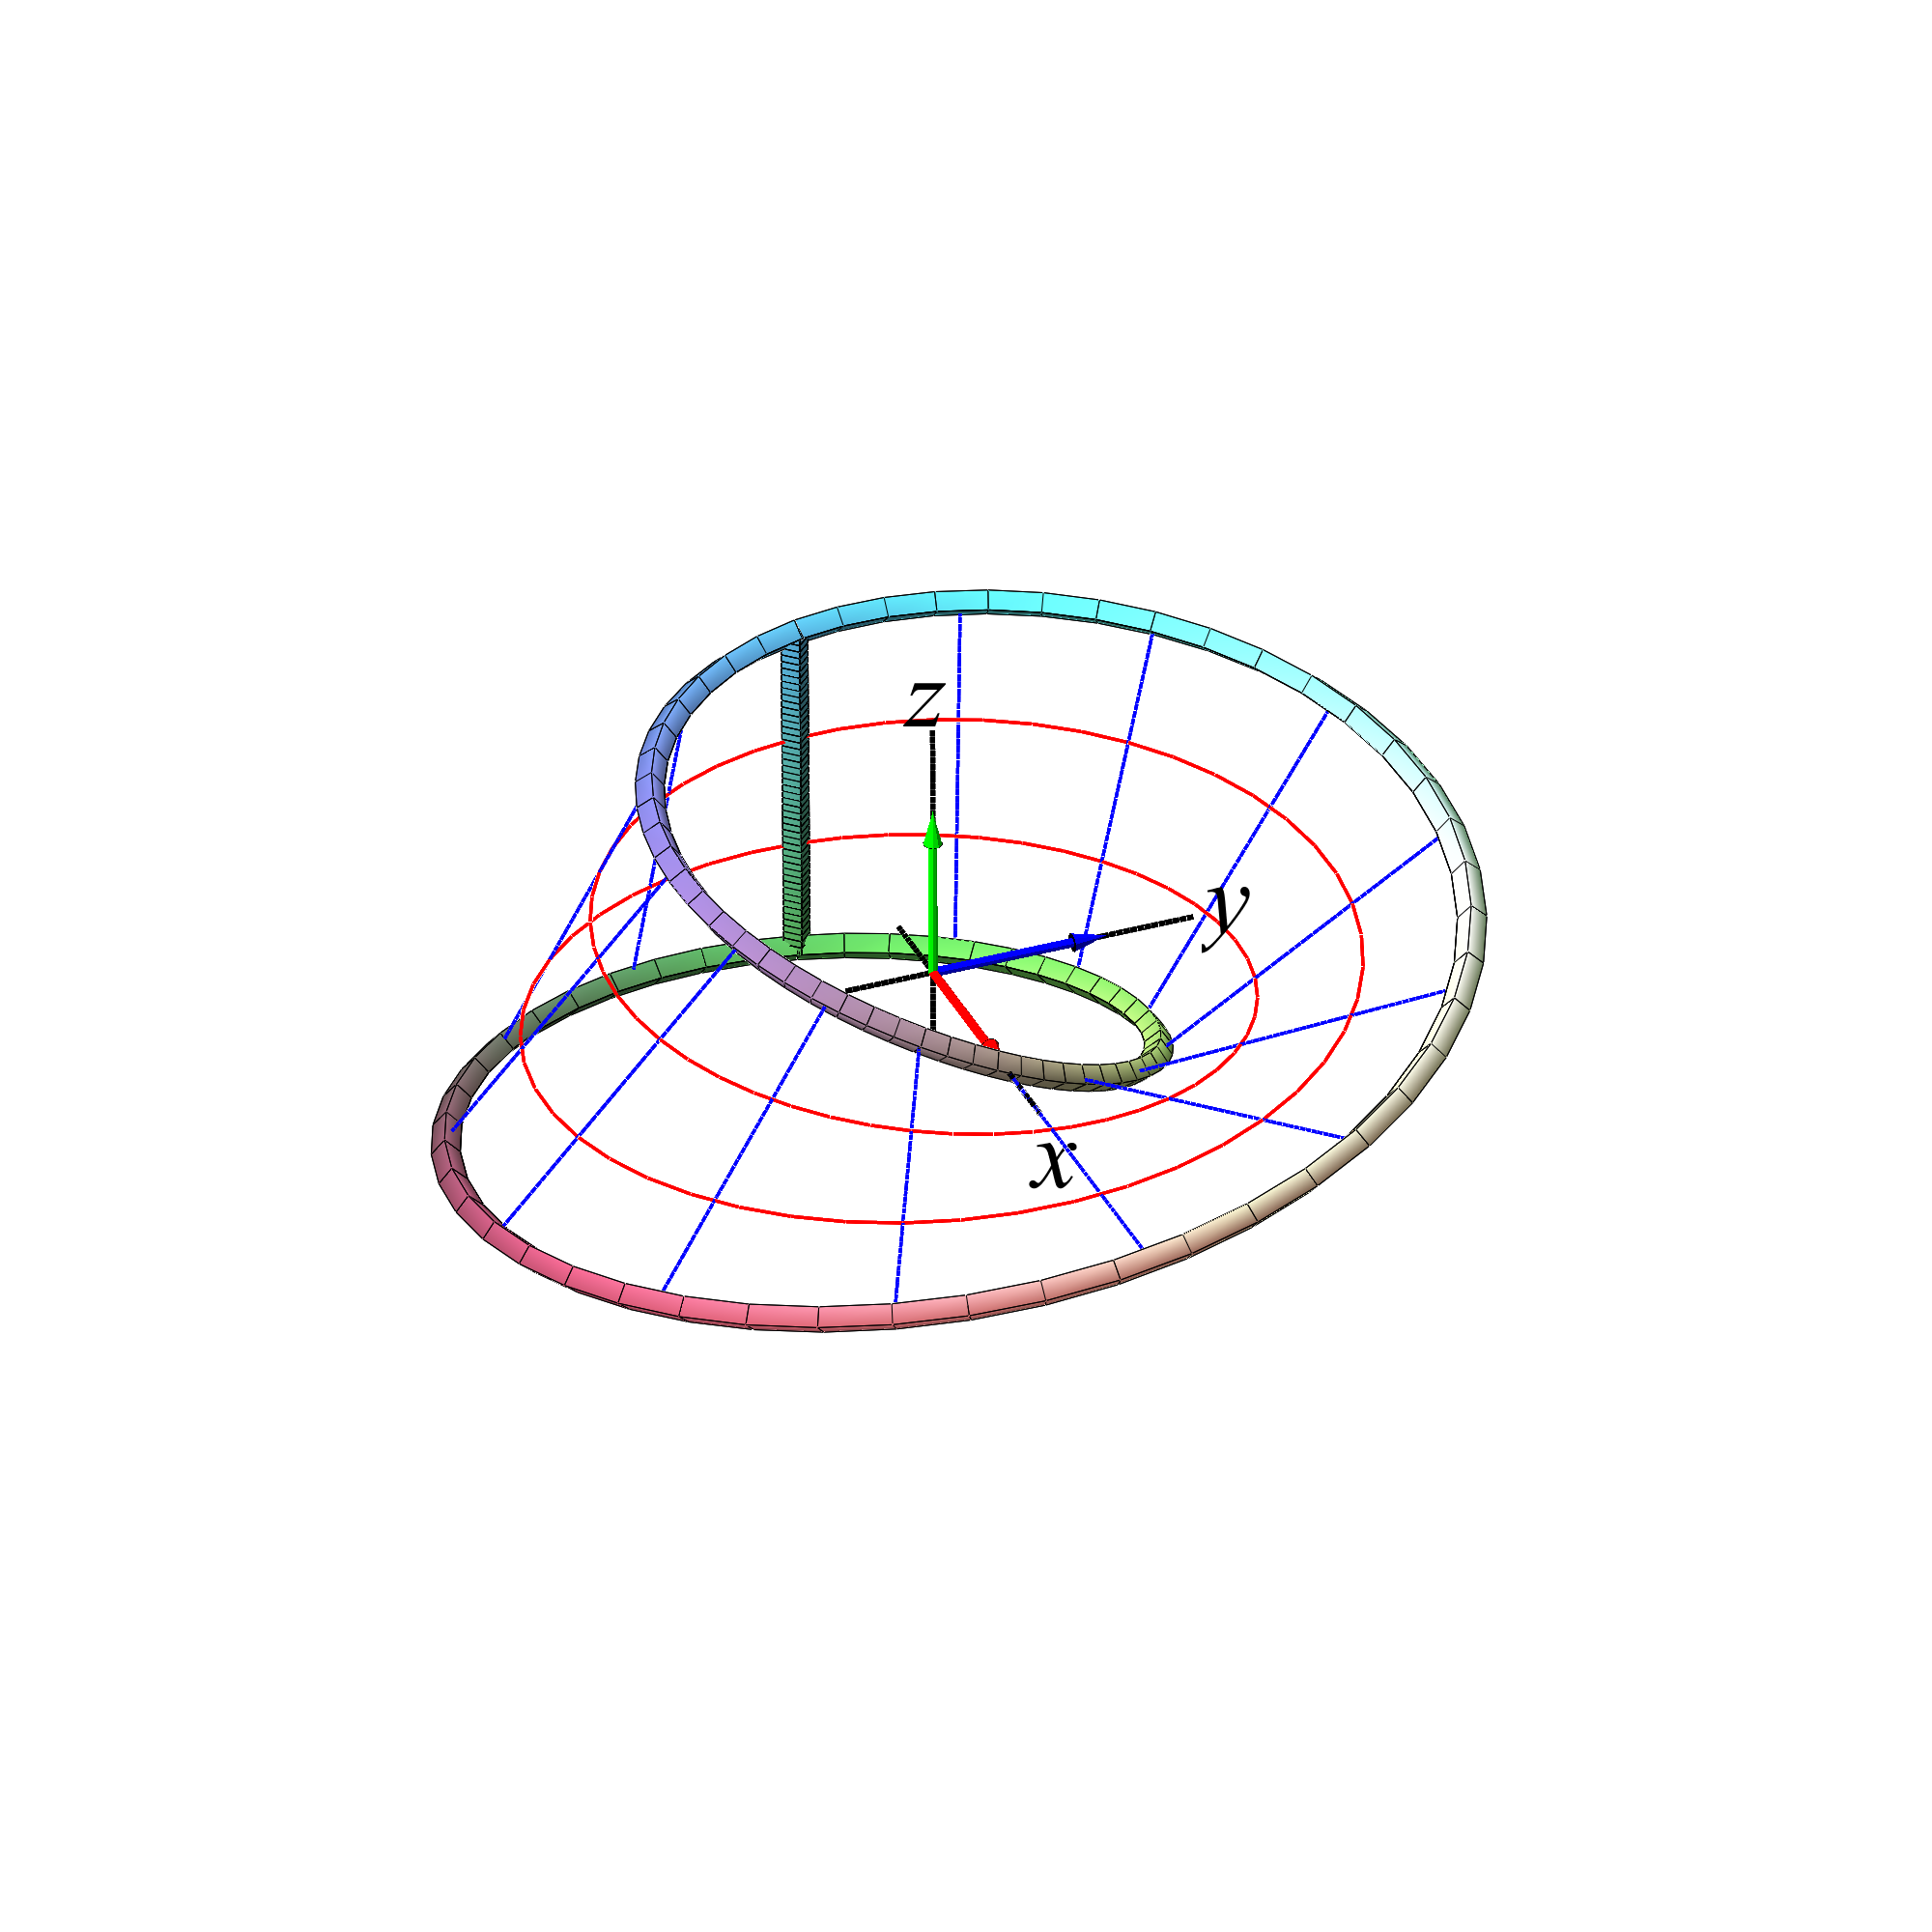
\includegraphics[height=70mm]{FIGS/plotMobius5}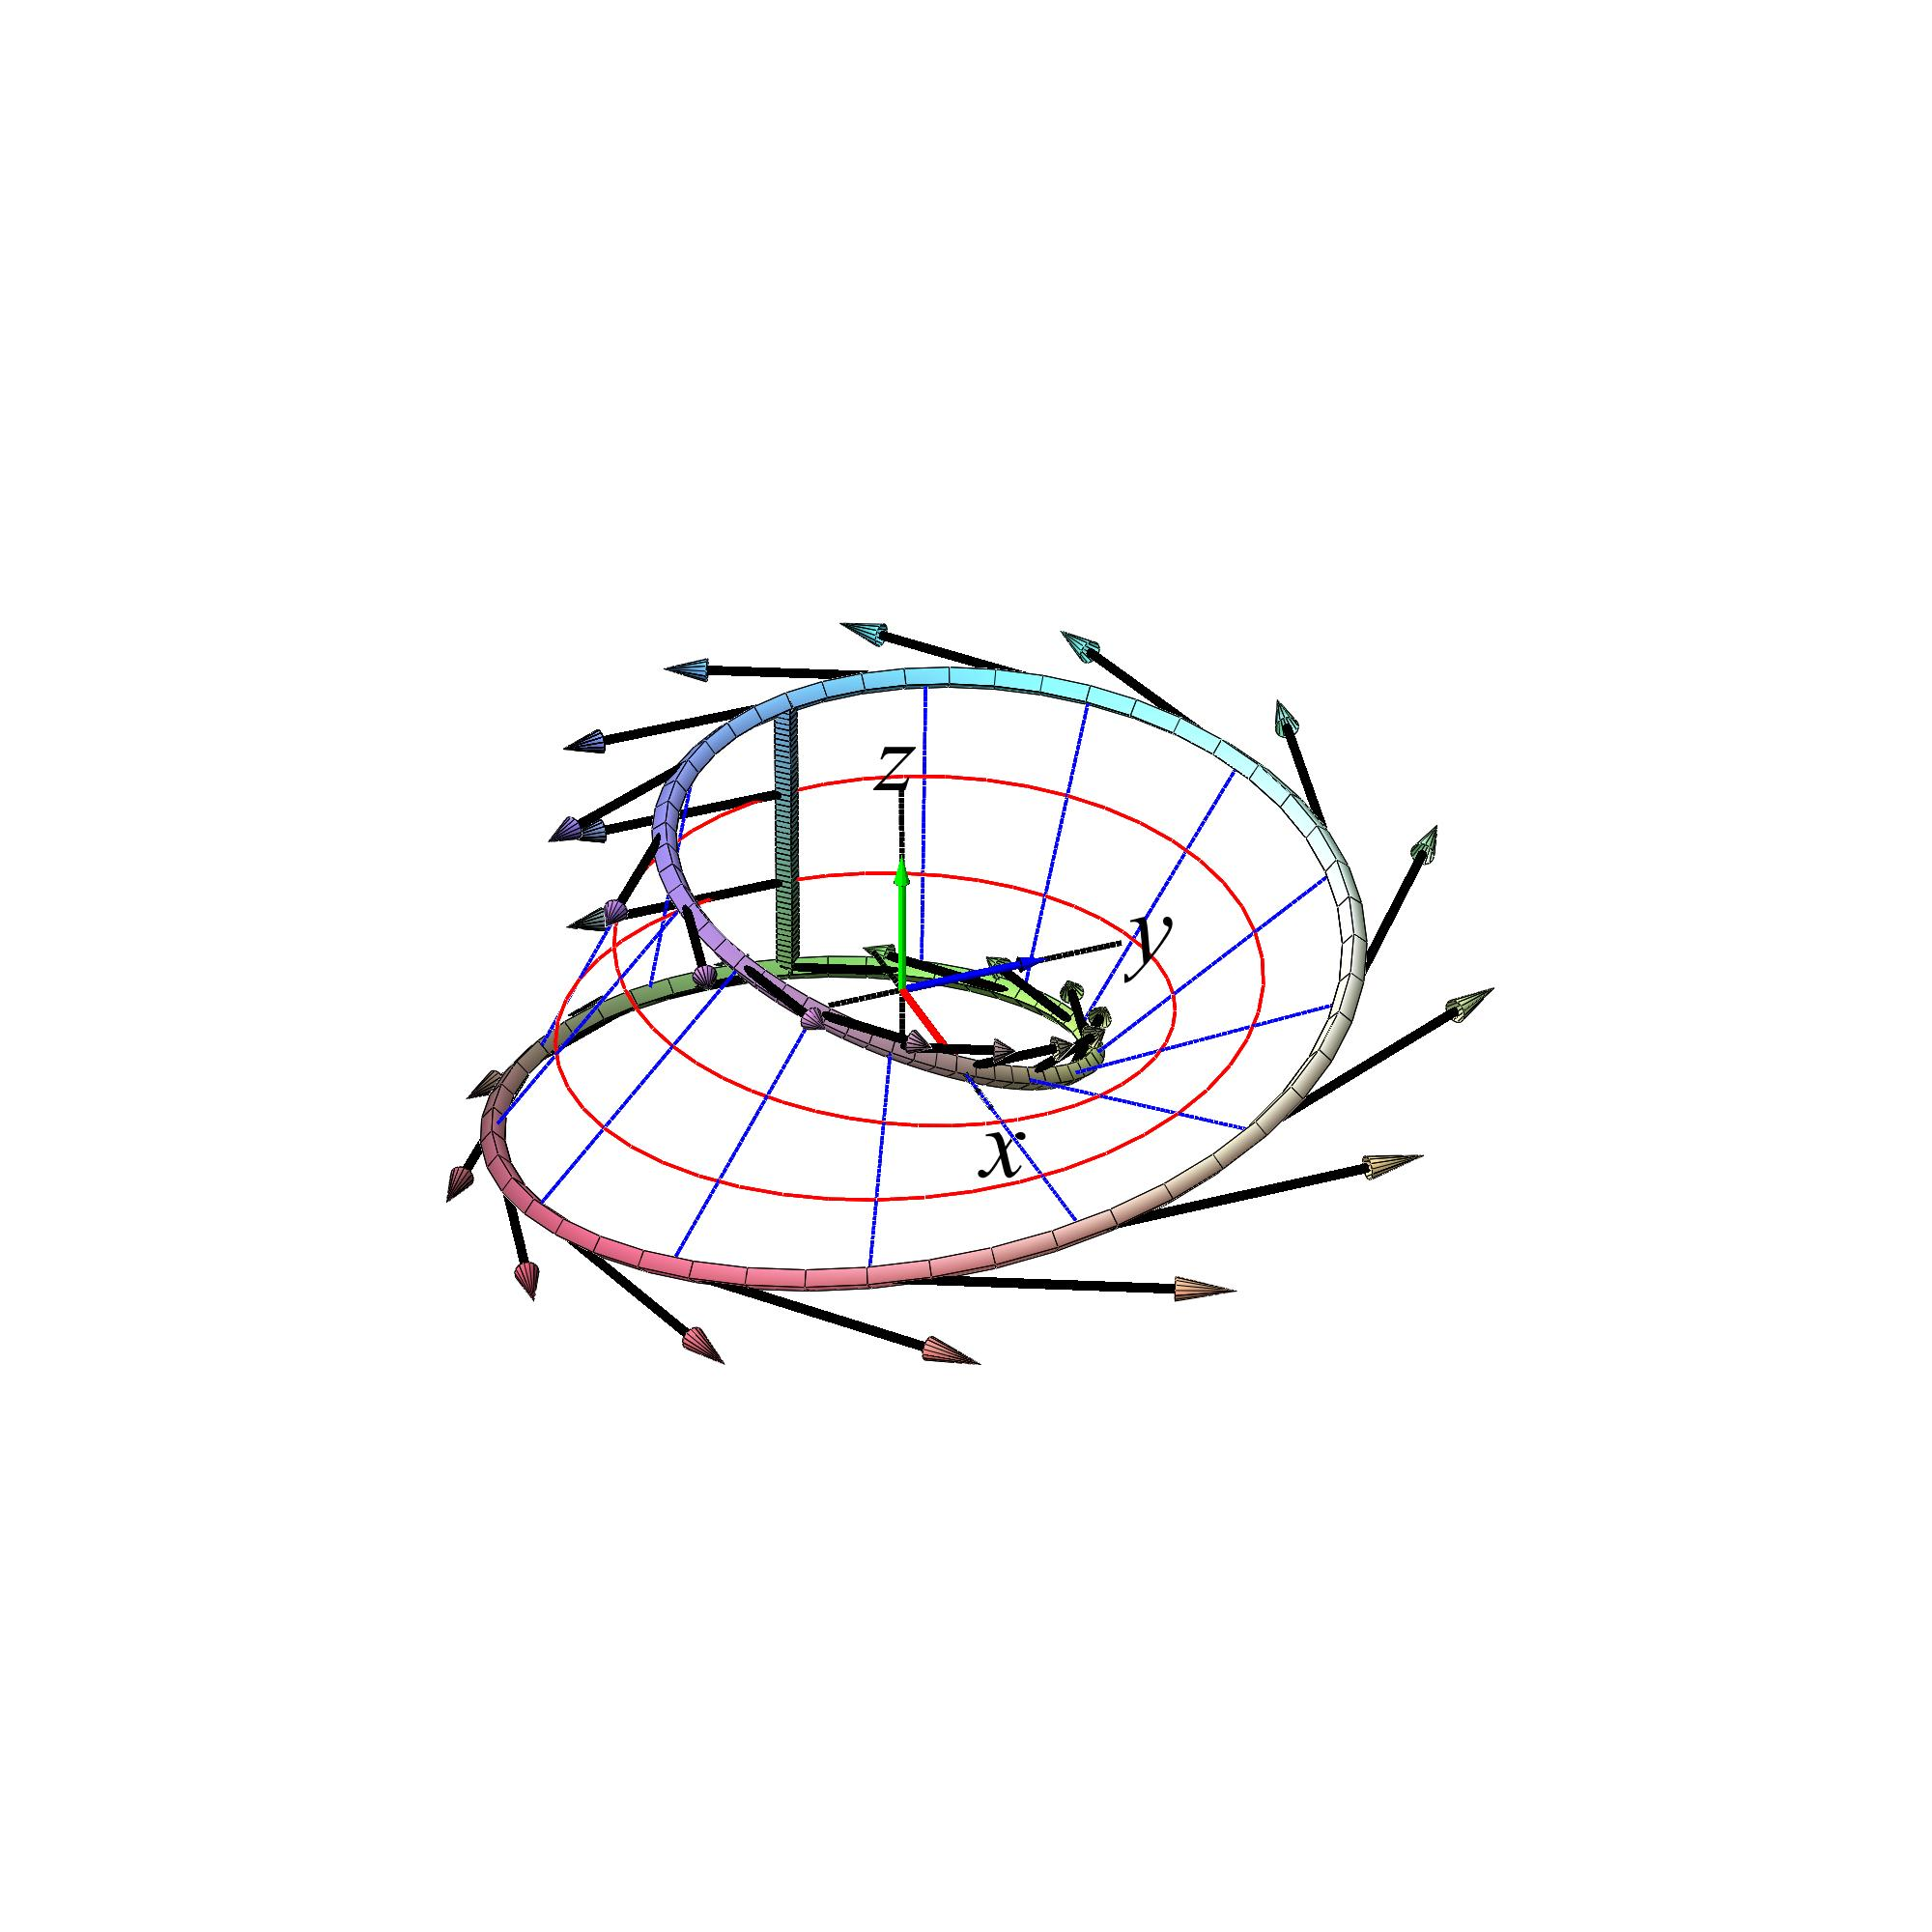
\includegraphics[height=70mm]{FIGS/plotMobius6}}
\begin{center}
\caption{\small{Restriktionen af  rotationsvektorfeltet $\Rot(\mathbf{V})(x,y,z)= (0, \, 0, \, 2)$ til et stykke af et M\"{o}bius bånd, båndets rand, og vektorfeltet $\mathbf{V}(x,y,z) = (-y, x, 1)$ restringeret til randen.}}
\label{figMob2}
\end{center}
\end{figure}




%%%%%%%%%%%%%%%%%%%%%%%%%%%%%%%%%%%%%%%%%%%%%%%%%%%%%%%%%%%%%%%%%%%%%%%%%%%%
%%%%%%%%%%%%%%%%%%%%%%%%%%%%%%%%%%%%%%%%%%%%%%%%%%%%%%%%%%%%%%%%%%%%%%%%%%%%
%%%%%%%%%%%%%%%%%%%%%%%%%%%%%%%%%%%%%%%%%%%%%%%%%%%%%%%%%%%%%%%%%%%%%%%%%%%%

\section{Stokes' sætning i planen} \label{secStokesInPlane}

Plane områder, for eksempel områder i $(x, y)-$planen, kan parametriseres således:
\begin{equation}
F_{\bf{r}}: \qquad  {\bf{r}}(u,v) \, = \,
(x(u,v), y(u,v), 0) \in \mathbb{R}^{3} \,\,
, \,\, (u,v) \in D\, = \, [a, b]\times[c, d]
\subset \mathbb{R}^{2} \quad.
\end{equation}

Et plant område har et særligt simpelt enhedsnormal-vektorfelt i rummet, dvs. når vi betragter
det plane område som en flade i rummet, der tilfældigvis ligger helt i $(x,y)-$planen:
$\mathbf{n}_{F} \, = \, (0, 0, 1)$. \\

Med hensyn til randen af det plane område repeterer vi notationen fra
afsnit \ref{secSurf}:
Randen $\partial F_{\bf{r}}$ af $F_{\bf{r}}$
fremkommer ved at bruge vektorfunktionen $\bf{r}$
på de 4 rette linjestykker, der udgør randen
$\partial D$ af det rektangulære parameterområde
$D\, = \, [a, b]\times[c, d]$. Vi parametriserer
hele $\partial D$ på \'{e}n gang ved hjælp af en
parameter $\theta$ og en vektor-funktion
$\bf{d}$:
$$
\partial D: \qquad  {\bf{d}}(\theta) \, = \, (u(\theta), v(\theta)) \in
\partial D \subset \mathbb{R}^{2} \,\, , \,\, \theta \in I \subset \mathbb{R} \quad,
$$
hvor $u(\theta)$ og $v(\theta)$ kun er stykkevis
differentiable funktioner af $\theta$. De kan
f.eks. vælges som lineære funktioner af $\theta$
for hvert enkelt  af de 4 linjestykker der udgør
$\partial D$.

Randen af $F_{\bf{r}}$ er så
\begin{equation}
\partial F_{\bf{r}}: \qquad  {\bf{b}}(\theta)\,
= \,{\bf{r}}({\bf{d}}(\theta)) \, = \,
{\bf{r}}(u(\theta), v(\theta)) \in
\mathbb{R}^{2} \subset \mathbb{R}^{3}\,\, , \,\, \theta \in I \, = \, [0, T] \subset
\mathbb{R} \quad.
\end{equation}


Lad nu $\,\mathbf{V}(x,y,z) \, = \, (V_{1}(x,y,z), V_{2}(x,y,z), V_{3}(x,y,z))\,$ betegne et vilkårligt vektorfelt i rummet, så har vi følgende konsekvens af Stokes' sætning:

\begin{theorem}[Stokes' sætning i planen] \label{thmStokesPlan}
Med ovenstående notation gælder:
\begin{equation}
\begin{aligned}
\int_{F_{\mathbf{r}}}\, \Rot({\bf{V}})\bm{\cdot} {\bf{n}}_{F} \,
\,d\mu \, &= \, \int_{\partial F} \, {\bf{V}}
\bm{\cdot} {\bf{e}}_{\partial F} \, d\mu \\
\int_{F_{\mathbf{r}}}\, \Rot({\bf{V}})\bm{\cdot} (0, 0, 1) \,
\,d\mu \, &= \, \int_{\partial F} \, (V_{1}, V_{2}, V_{3})
\bm{\cdot} {\bf{e}}_{\partial F} \, d\mu \\
\int_{F_{\mathbf{r}}}\, \Rot({\bf{V}})\bm{\cdot} (0, 0, 1) \,
\,d\mu \, &= \, \int_{I} \, (V_{1}, V_{2}, V_{3})
\bm{\cdot} {\mathbf{b}}'(\theta)\, d\theta \\
\int_{F_{\mathbf{r}}}\, \left( \frac{\partial V_{2}}{\partial x} -  \frac{\partial V_{1}}{\partial y}\right) \,
\,d\mu \, &= \, \int_{0}^{T} \,\left( V_{1}b_{1}'(\theta) +  V_{2}b_{2}'(\theta) \right) \,d\theta \quad ,
\end{aligned}
\end{equation}
og dermed
\begin{equation} \label{eqStokesPlan}
\int_{c}^{d}\int_{a}^{b}\, \left( \frac{\partial V_{2}}{\partial x} -  \frac{\partial V_{1}}{\partial y}\right) \, \Jac_{\mathbf{r}}(u,v)\,
\,du \, dv \, = \, \int_{0}^{T} \, \left( V_{1}b_{1}'(\theta) +  V_{2}b_{2}'(\theta)\right) \,d\theta \quad .
\end{equation}
\end{theorem}

\begin{remark}
Det ses, at vektorfeltets tredie koordinat-funktion $V_{3}(x,y,z)$ ikke spiller nogen rolle i sætningen. Sætningen er derfor et resultat om vektorfunktioner i {\em{planen}}: $\,\mathbf{V}(x,y) \, = \, \left(V_{1}(x,y), V_{2}(x,y)\right)\,$. Vi illustrerer med et detaljeret - men simpelt - eksempel nedenfor.
\end{remark}



\begin{example}[Stokes' sætning i planen] \label{exampStokesPlane}
Lad $\,\mathbf{V}(x,y) \, = \, \left( -y, x \right) \,$ og  $\mathbf{r}(u,v) \, = \, (3u, 4v)$, $u \in [a,b]$, $v \in [c,d]$,  så får vi:
$\Jac_{\mathbf{r}}(u,v)\, = \, 12$ og $\frac{\partial V_{2}}{\partial x} -  \frac{\partial V_{1}}{\partial y} \, = \, 2$ sådan at venstre side i ligning (\ref{eqStokesPlan}) giver:
\begin{equation} \label{eqStokesPlanEx}
\begin{aligned}
&\int_{c}^{d}\int_{a}^{b}\, \left( \frac{\partial V_{2}}{\partial x} -  \frac{\partial V_{1}}{\partial y}\right) \, \Jac_{\mathbf{r}}(u,v)\,
\,du \, dv \\
&= \int_{c}^{d}\int_{a}^{b}\, 2\cdot 12 \,
\,du \, dv \\
&= \, 24(b-a)(d-c) \quad .
\end{aligned}
\end{equation}
Højre side i ligning (\ref{eqStokesPlan}) skal give samme værdi.\\

Vi bestemmer  højre sides værdi ved at opdele randen af $F_{\bf{r}}$ i 4 retlinede komponenter og ved at beregne det tangentielle kurveintegral af $\mathbf{V}$ langs hver komponent, idet vi i hvert tilfælde sørger for at orientere (parametrisere) komponenten korrekt efter den forskrift, som er præciseret i Stokes' sætning. \\

Vi begynder med at sætte $T \, = \, 2(b-a) + 2(d-c)$, dvs. $T$ er den totale omkreds af parameterområdet $D$. Randen af $D$ kan vi så parametrisere på følgende måde:
\begin{equation}
\begin{aligned}
\mathbf{d}(\theta) \, &= \, (a + \theta \, , \,\, 0)\, \quad \textrm{for} \quad \theta \in [0\, , \,\, b-a] \\
\mathbf{d}(\theta) \, &= \, (b \, , \,\, c + \theta)\, \quad \textrm{for} \quad \theta \in [b-a\, , \,\, b-a + d-c] \\
\mathbf{d}(\theta) \, &= \, (b - \theta\, , \,\, d)\, \quad \textrm{for} \quad \theta \in [b-a + d-c\, , \,\, 2(b-a) + d-c] \\
\mathbf{d}(\theta) \, &= \, (a\, , \,\, d - \theta)\, \quad \textrm{for} \quad \theta \in [2(b-a) + d-c\, , \,\, 2(b-a) + 2(d-c)] \quad .
\end{aligned}
\end{equation}
Randen af $F_{\mathbf{r}}$ har vi dernæst på følgende form:
\begin{equation}
\begin{aligned}
\mathbf{b}(\theta) \, &= \, (3(a + \theta) \, , \,\, 0)\, \quad \textrm{for} \quad \theta \in [0\, , \,\, b-a] \\
\mathbf{b}(\theta) \, &= \, (3b \, , \,\, 4(c + \theta))\, \quad \textrm{for} \quad \theta \in [b-a\, , \,\, b-a + d-c] \\
\mathbf{b}(\theta) \, &= \, (3(b - \theta)\, , \,\, 4d)\, \quad \textrm{for} \quad \theta \in [b-a + d-c\, , \,\, 2(b-a) + d-c] \\
\mathbf{b}(\theta) \, &= \, (3a\, , \,\, 4(d - \theta))\, \quad \textrm{for} \quad \theta \in [2(b-a) + d-c\, , \,\, 2(b-a) + 2(d-c)] \quad ,
\end{aligned}
\end{equation}
og dermed:
\begin{equation}
\begin{aligned}
\mathbf{b}'(\theta) \, &= \, (3 \, , \,\, 0)\, \quad \textrm{for} \quad \theta \in [0\, , \,\, b-a] \\
\mathbf{b}'(\theta) \, &= \, (0 \, , \,\, 4)\, \quad \textrm{for} \quad \theta \in [b-a\, , \,\, b-a + d-c] \\
\mathbf{b}'(\theta) \, &= \, (-3\, , \,\, 0)\, \quad \textrm{for} \quad \theta \in [b-a + d-c\, , \,\, 2(b-a) + d-c] \\
\mathbf{b}'(\theta) \, &= \, (0\, , \,\, -4)\, \quad \textrm{for} \quad \theta \in [2(b-a) + d-c\, , \,\, 2(b-a) + 2(d-c)] \quad .
\end{aligned}
\end{equation}



Vi kan nu beregne højresiden i ligning (\ref{eqStokesPlan}) som summen af de 4 led, der stammer fra hver sin komponent af randkurven. For eksempel, for det første linjestykke i randkurven, som er parallel med $x-$aksen og med konstant $y=4c$ har vi:  $\theta \in [0, b-a]$ har vi $b_{1}'(\theta) = 3$,  $b_{2}'(\theta) = 0$, $V_{1}(x,y) = y = b_{2}(u,v) = 4v = 4c$ og ligeledes for de andre 3 bidrag (se figurerne \ref{figFlatStokesA} og \ref{figFlatStokesB}):
\begin{equation}
\begin{aligned}
\int_{0}^{T} \, V_{1}b_{1}'(\theta) &+  V_{2}b_{2}'(\theta) \,\,d\theta \, = \\ \,
& \phantom{+}\, \int_{0}^{b-a} \,12c \,\,d\theta  \,  \\
& +\, \int_{b-a}^{b-a+d-c} \, 12b\,\,d\theta   \, \\
& +\, \int_{b-a+d-c}^{2(b-a)+d-c} \, 12d \,\,d\theta   \,  \\
& +\, \int_{2(b-a) + d-c }^{2(b-a) + 2(d-c) } \, 12a \,\,d\theta  \, \\ = \\
&\phantom{+}\, 12c(b-a)\\
& +\, 12b(d-c)\\
& +\, 12d(b-a)\\
& +\, 12a(d-c) \, \\ = \\
& \phantom{+}\, 24(b-a)(d-c) \quad,
\end{aligned}
\end{equation}
i overensstemmelse med resultatet i ligning (\ref{eqStokesPlanEx}), sådan at den generelle ligning (\ref{eqStokesPlan}) dermed er verificeret i dette tilfælde.

\end{example}


\begin{figure}[h]
\centerline{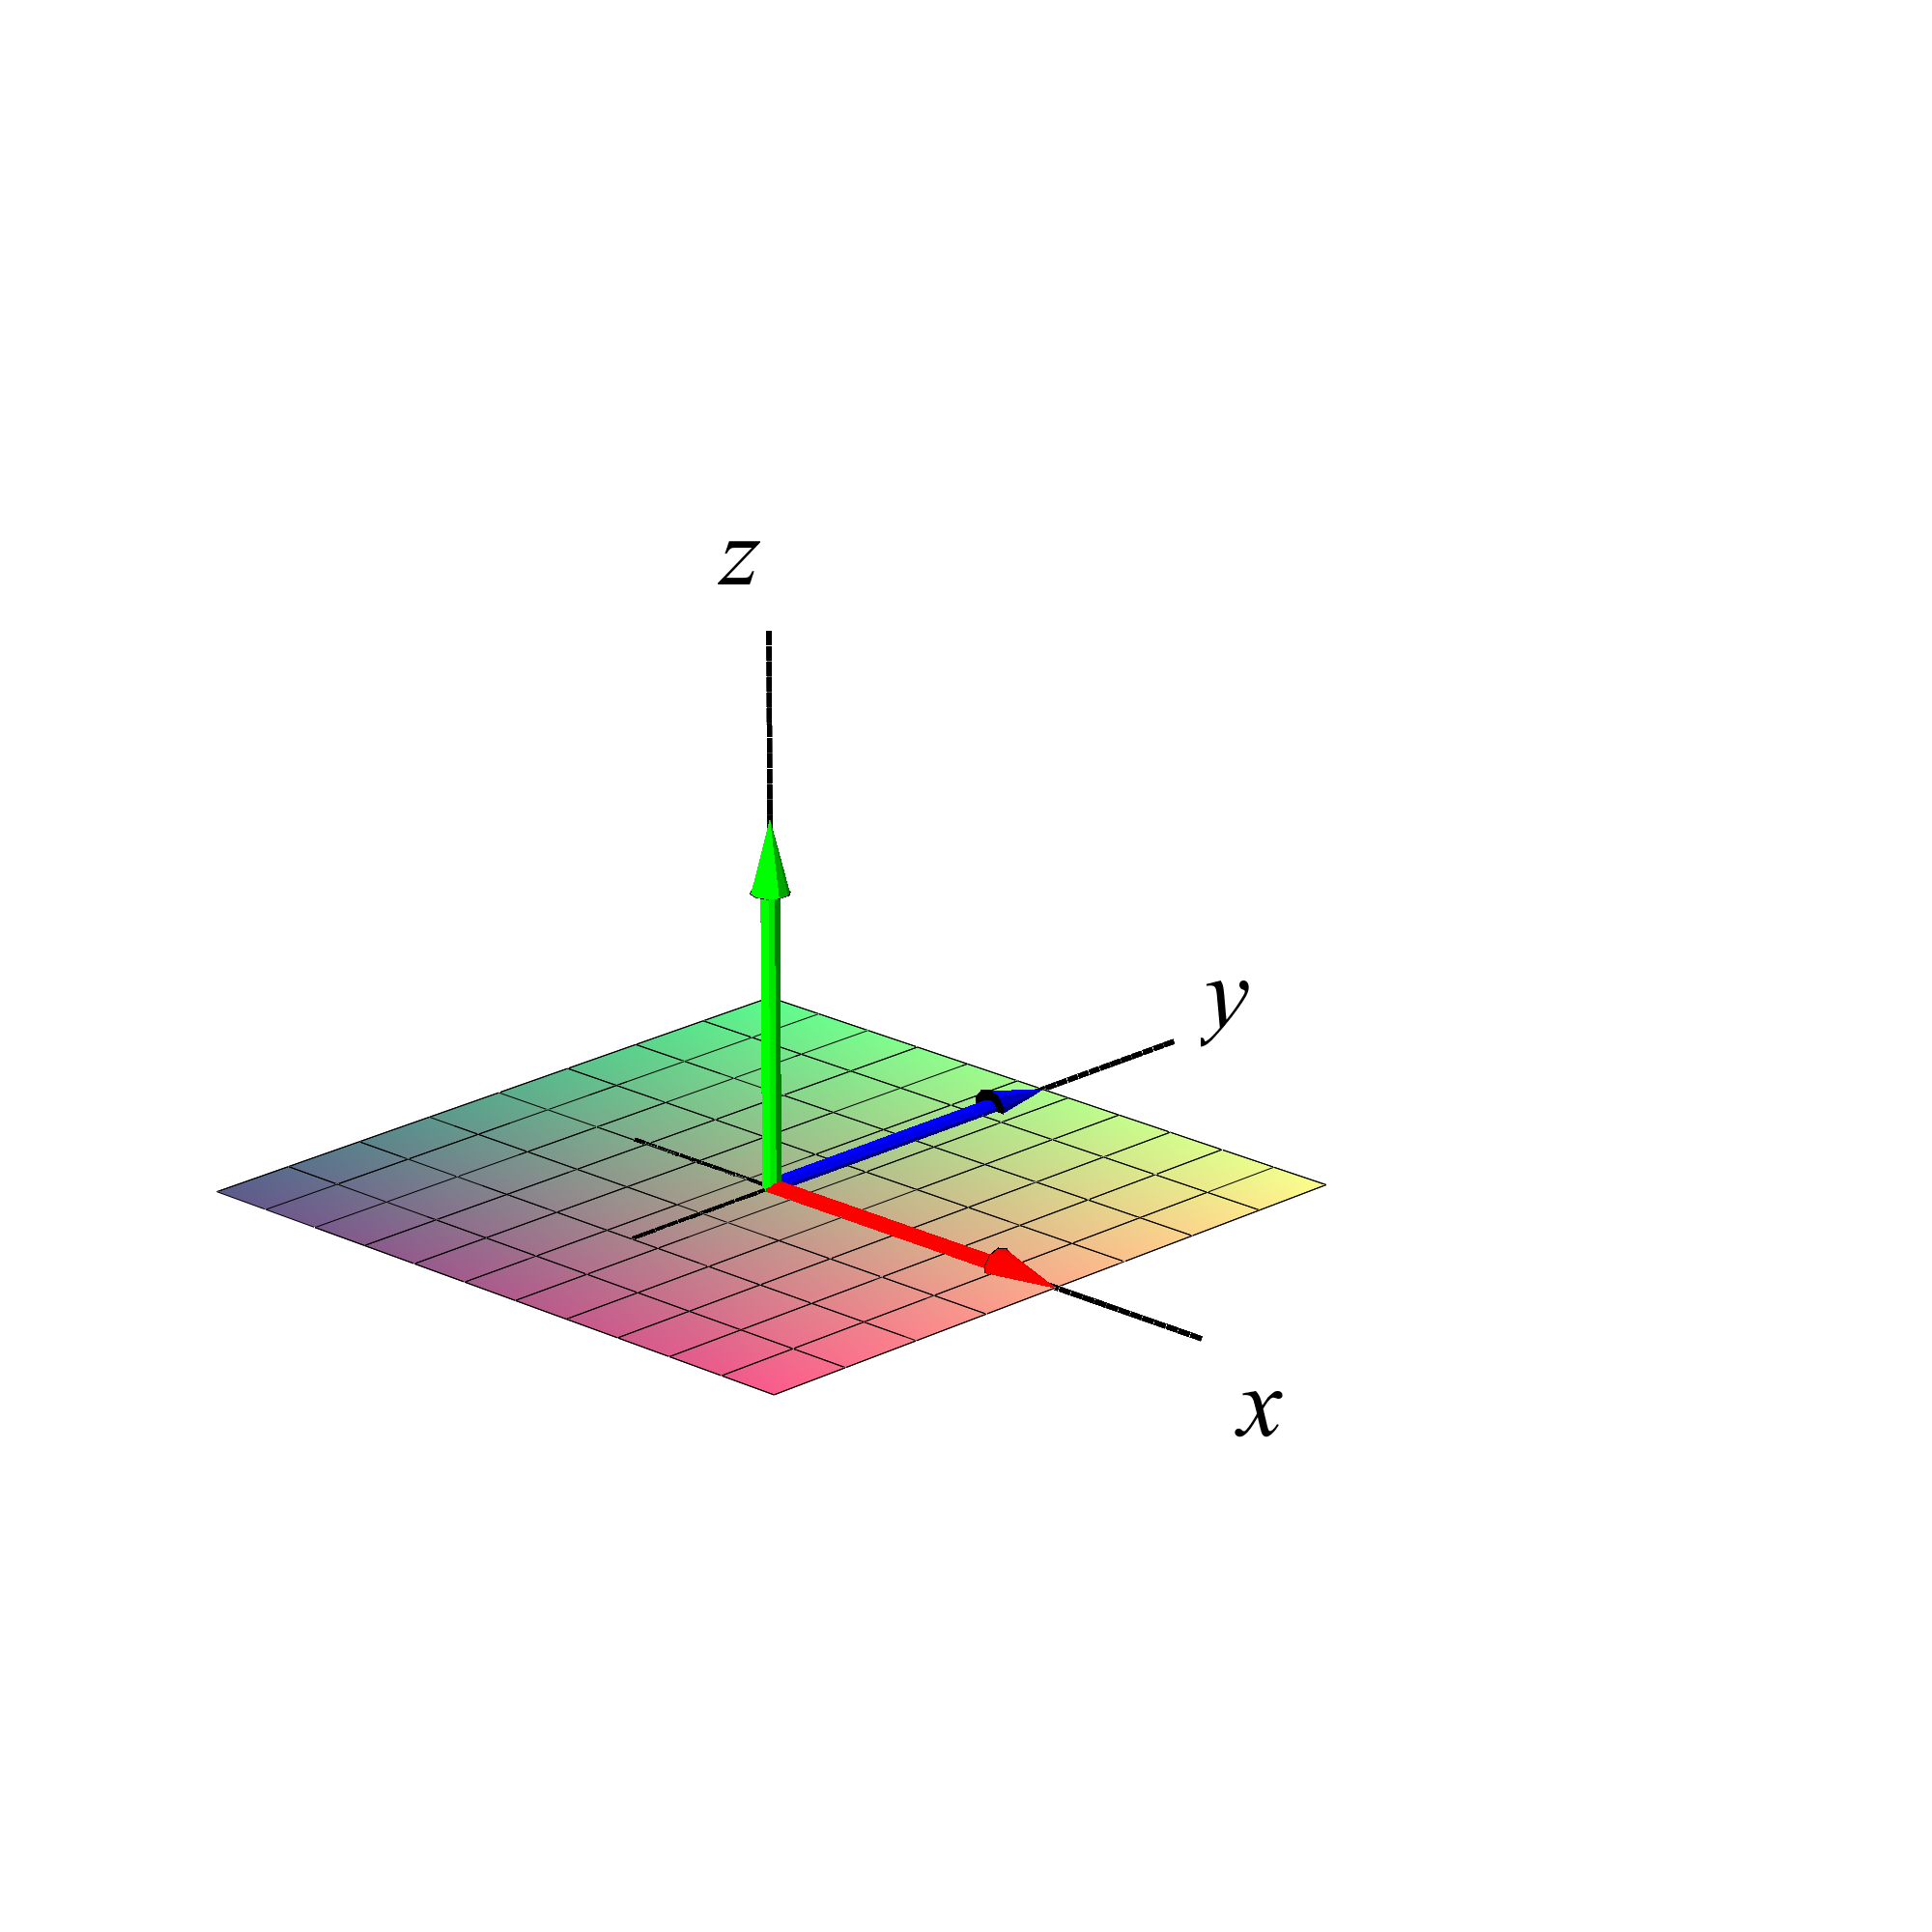
\includegraphics[height=70mm]{FIGS/plotFlat1}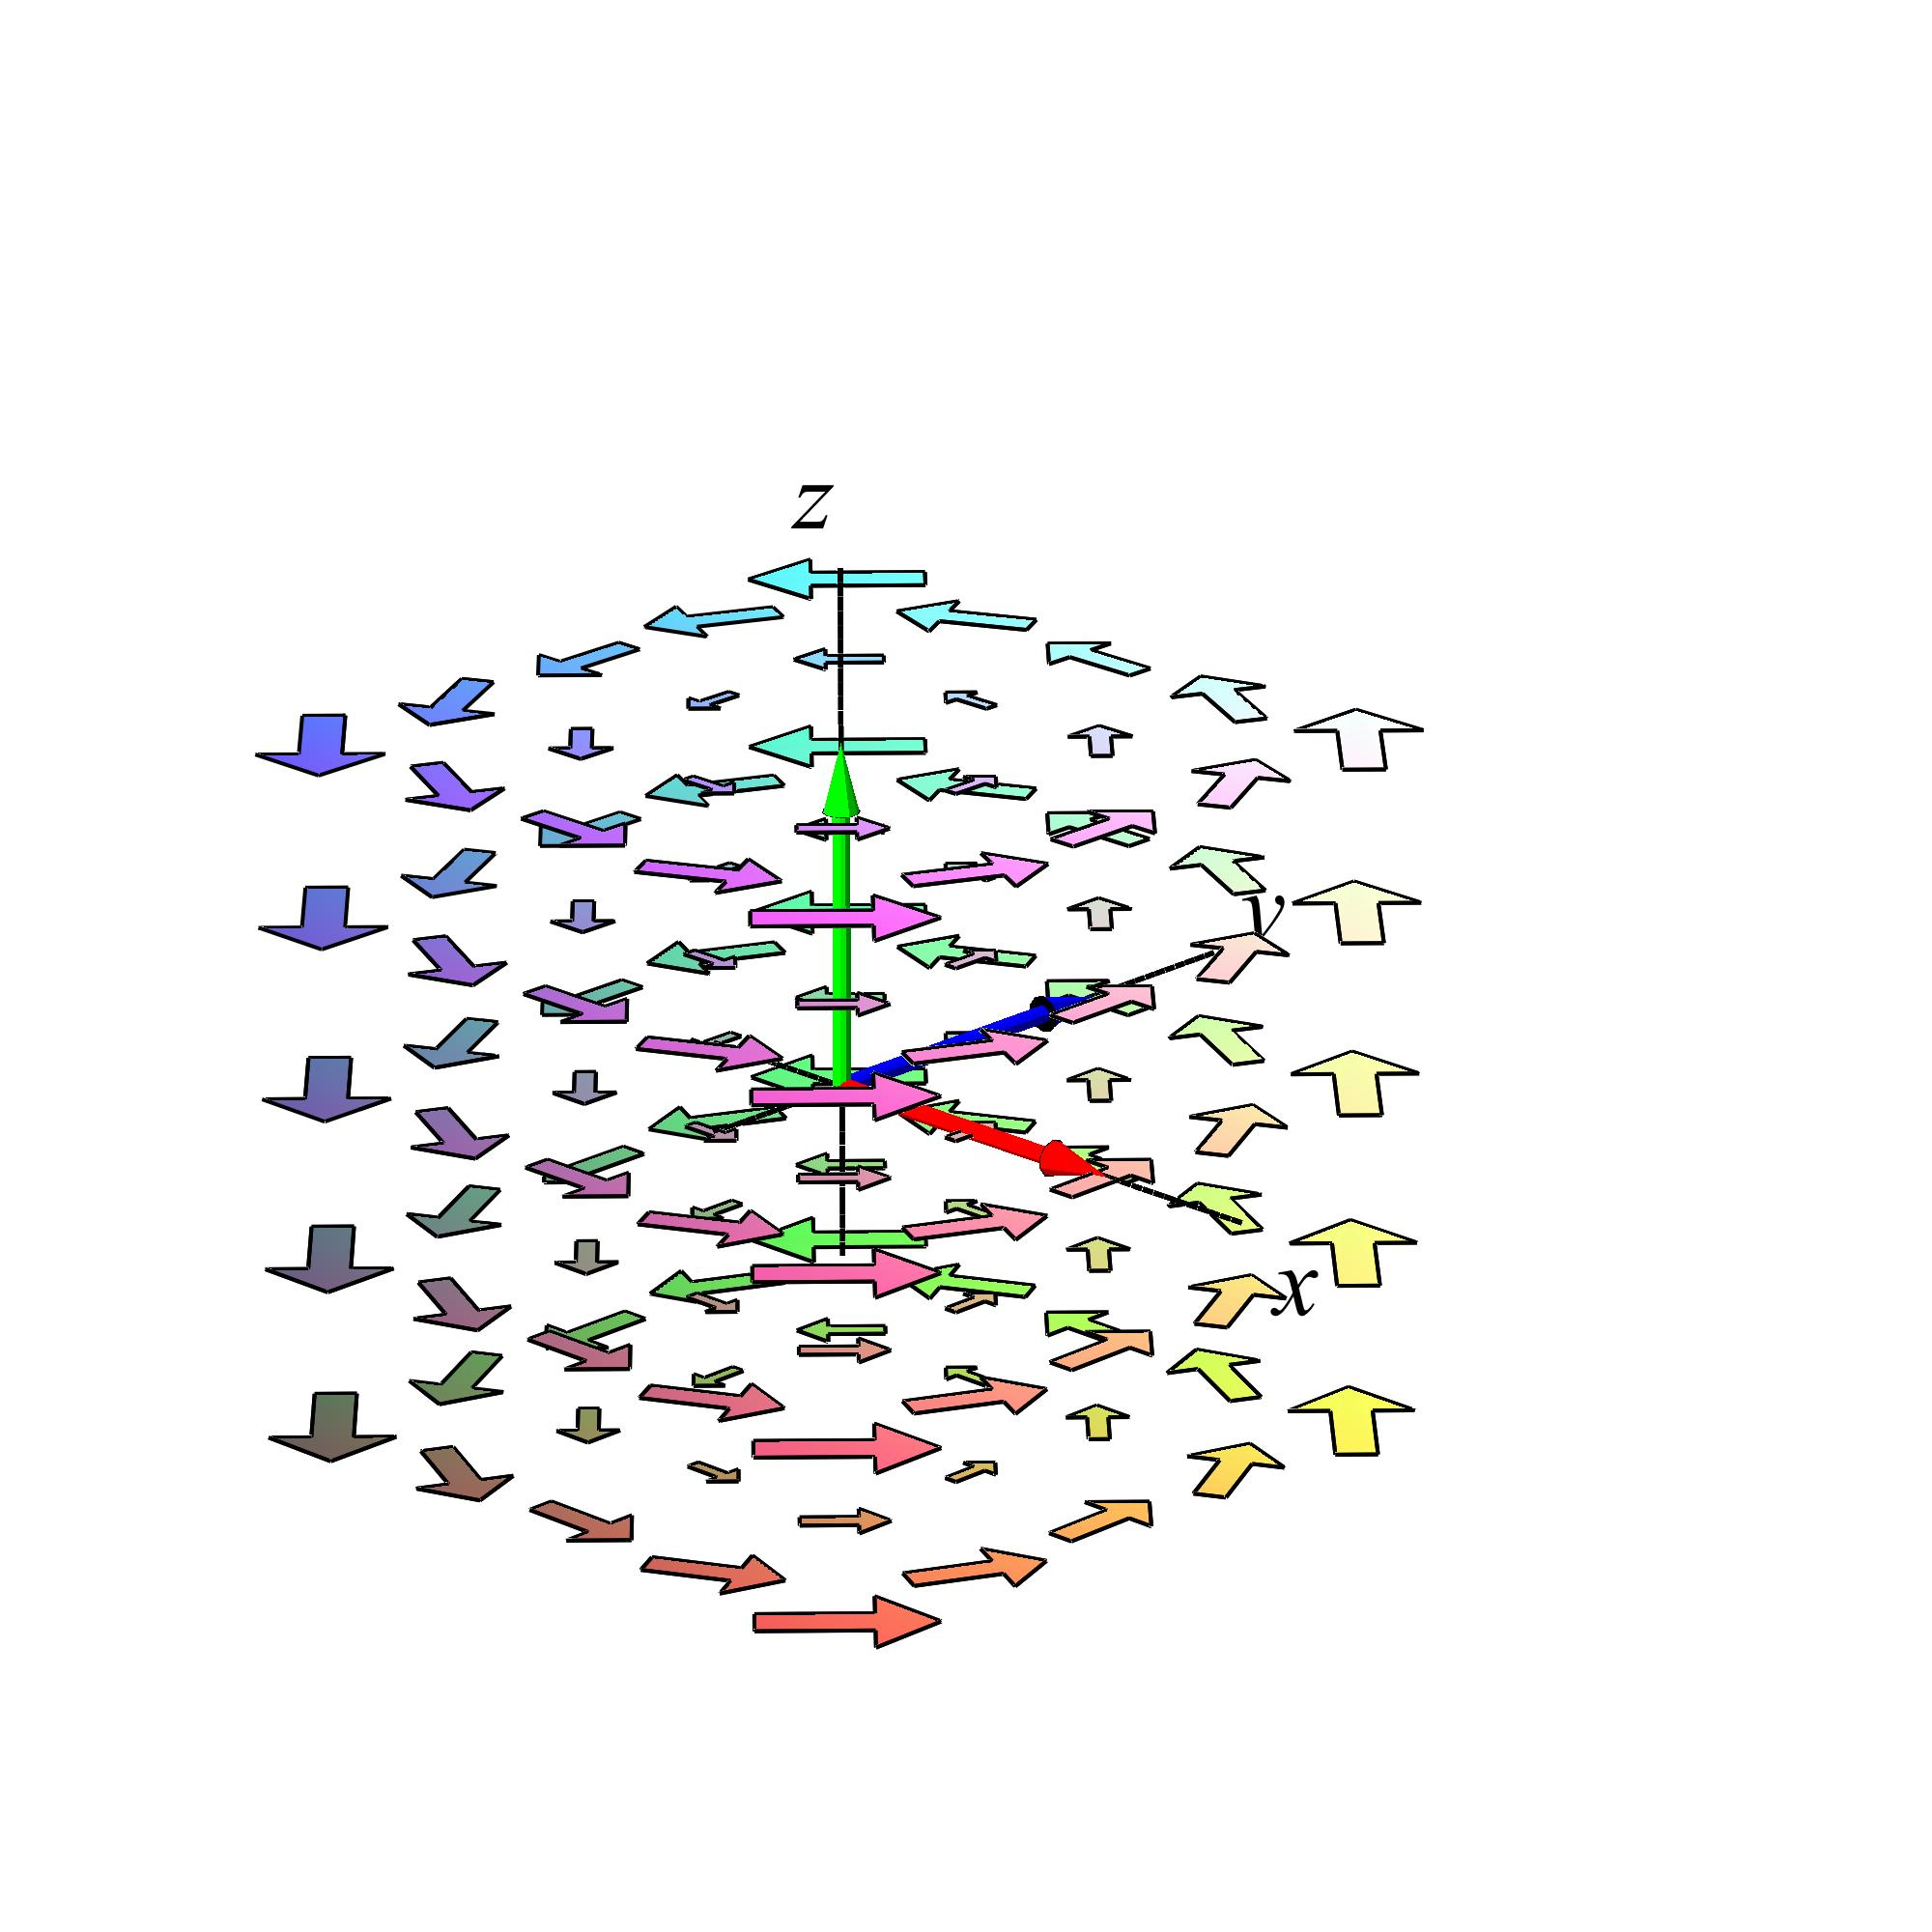
\includegraphics[height=70mm]{FIGS/plotFlat2}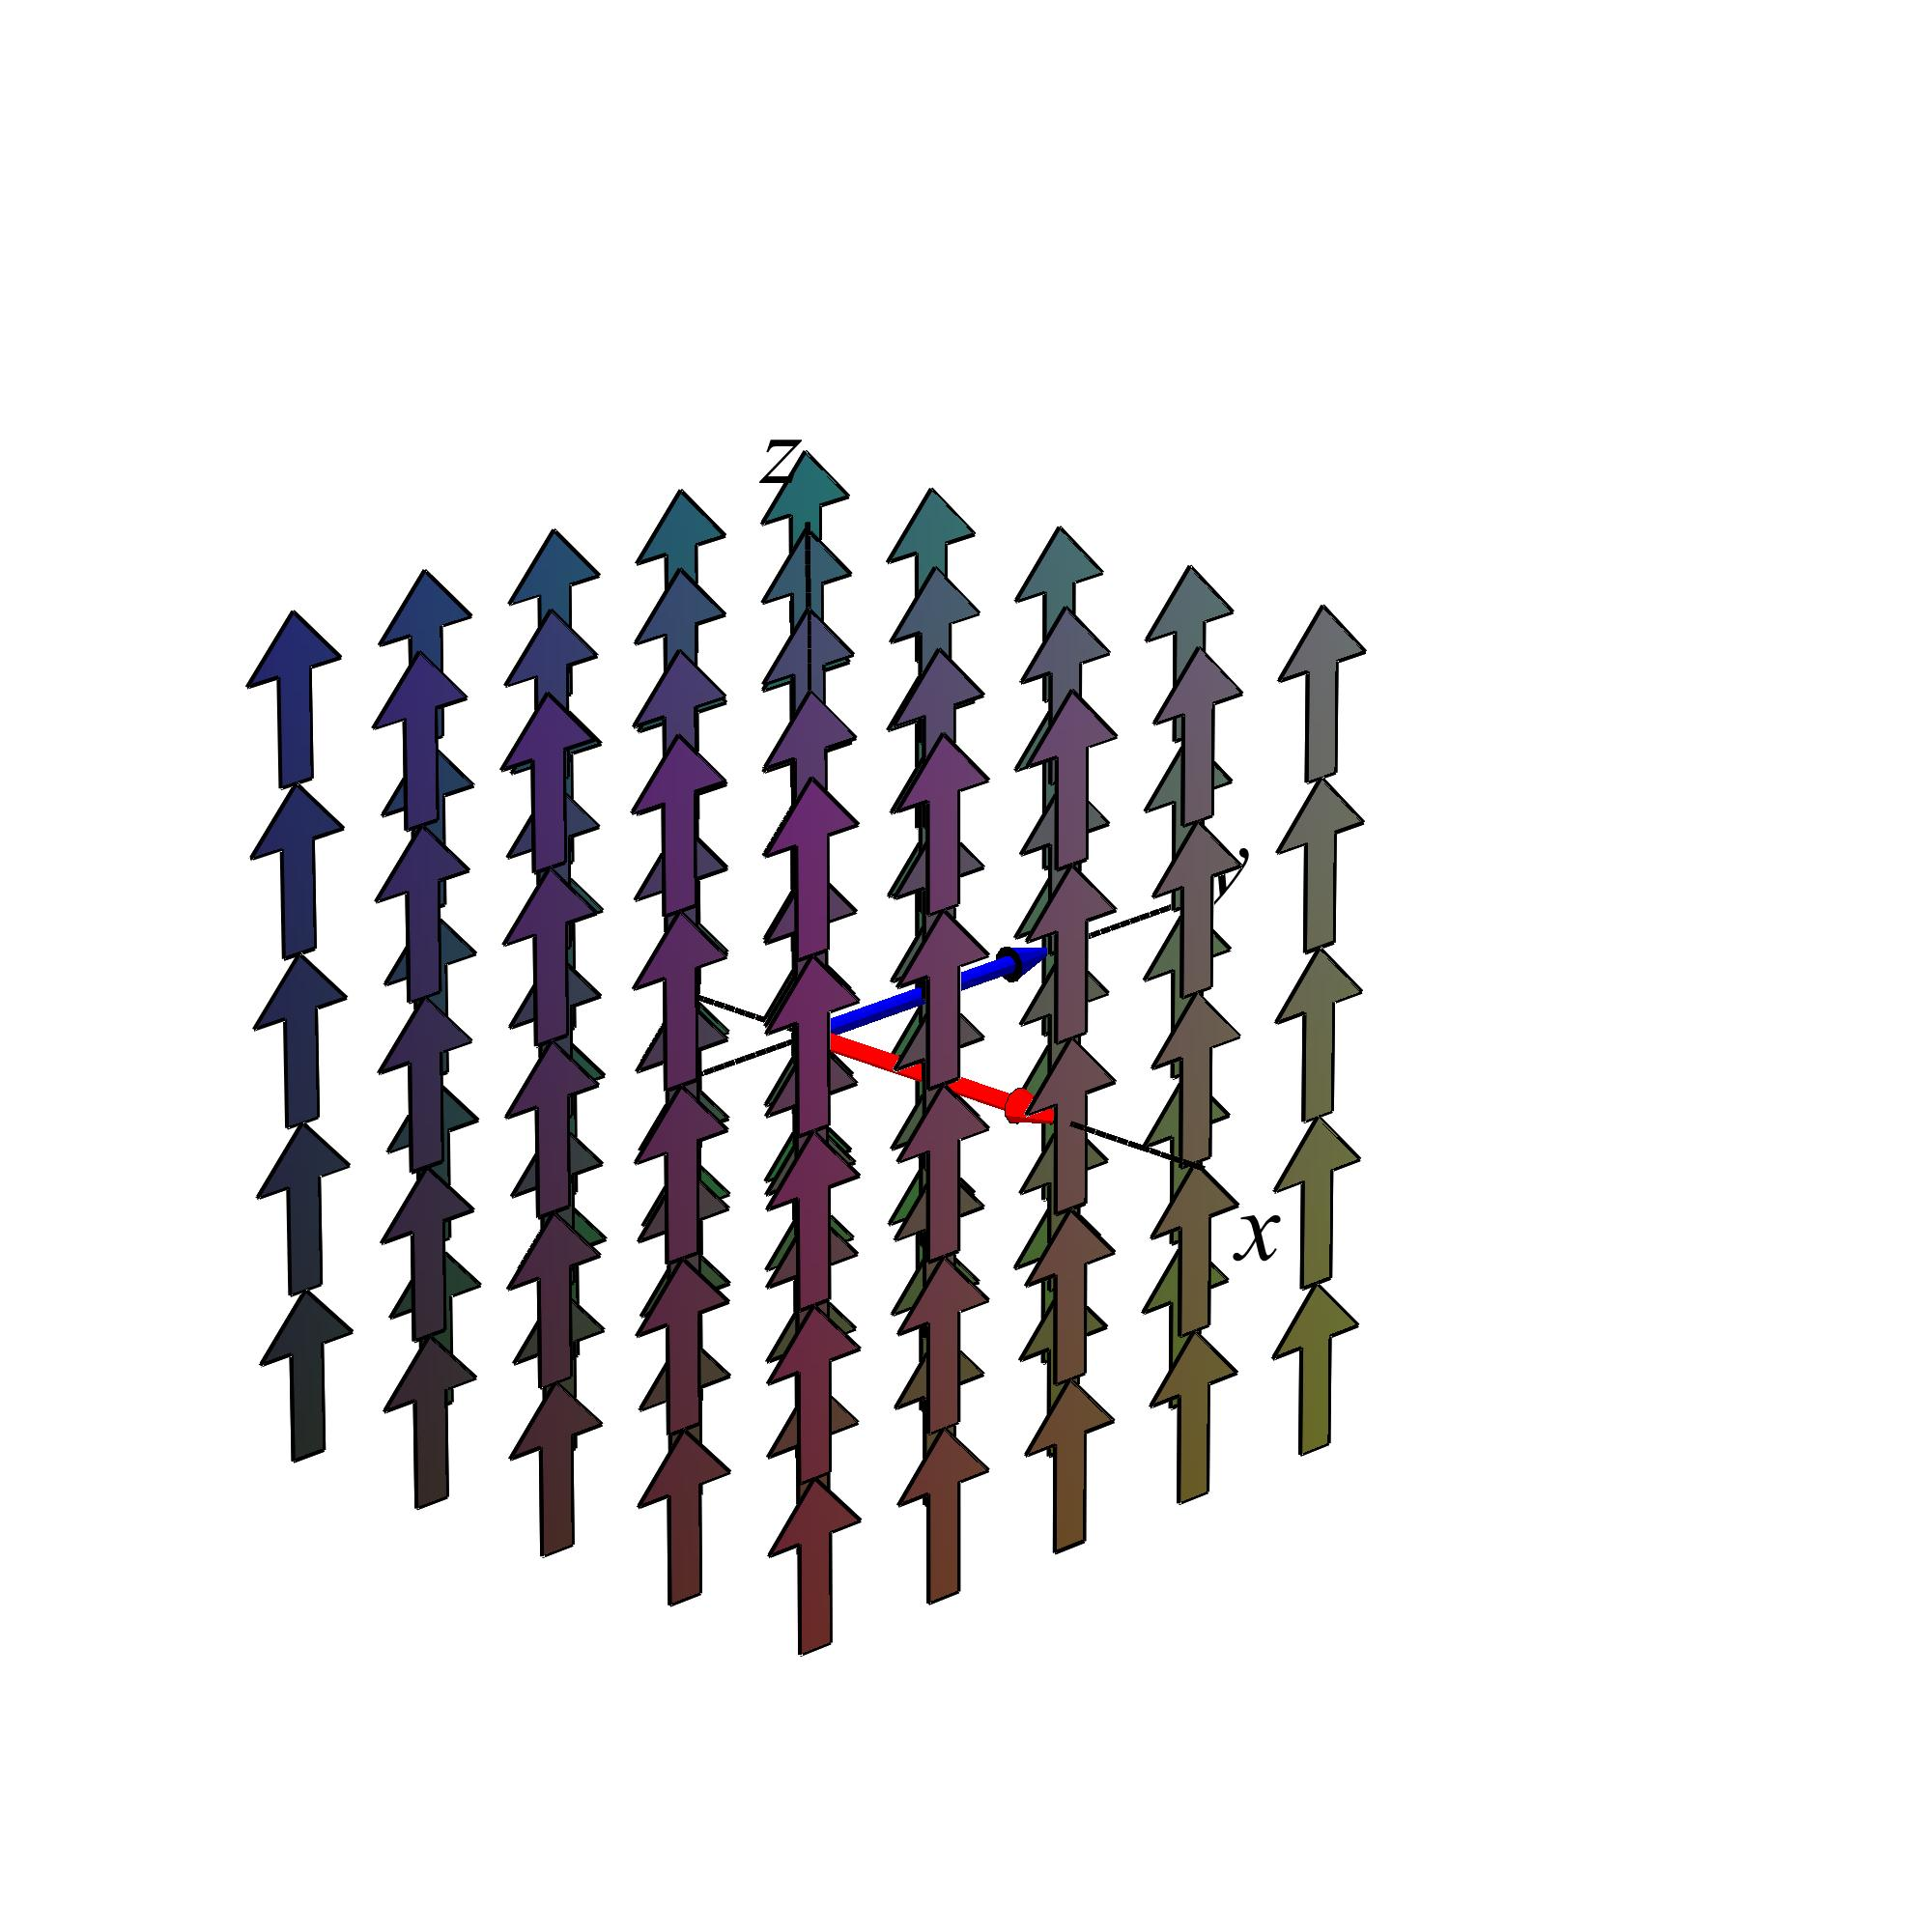
\includegraphics[height=70mm]{FIGS/plotFlat3}}
\begin{center}
\caption{\small{3D versionering af eksempel \ref{exampStokesPlane}. Vektorfeltet $\mathbf{V}(x,y) = (-y, x, 0)$ har rotationsvektorfeltet $(0,0,2)$. Her er valgt et kvadrat med parameterfremstilling $\mathbf{r}(u,v) = (3u,\, 4v, 0)\,$, $u \in [a, b]$, $v \in [c,d]$, $a=-1/3$, $b=1/3$, $c=-1/4$, og $d=1/4$.}}
\label{figFlatStokesA}
\end{center}
\end{figure}


\begin{figure}[h]
\centerline{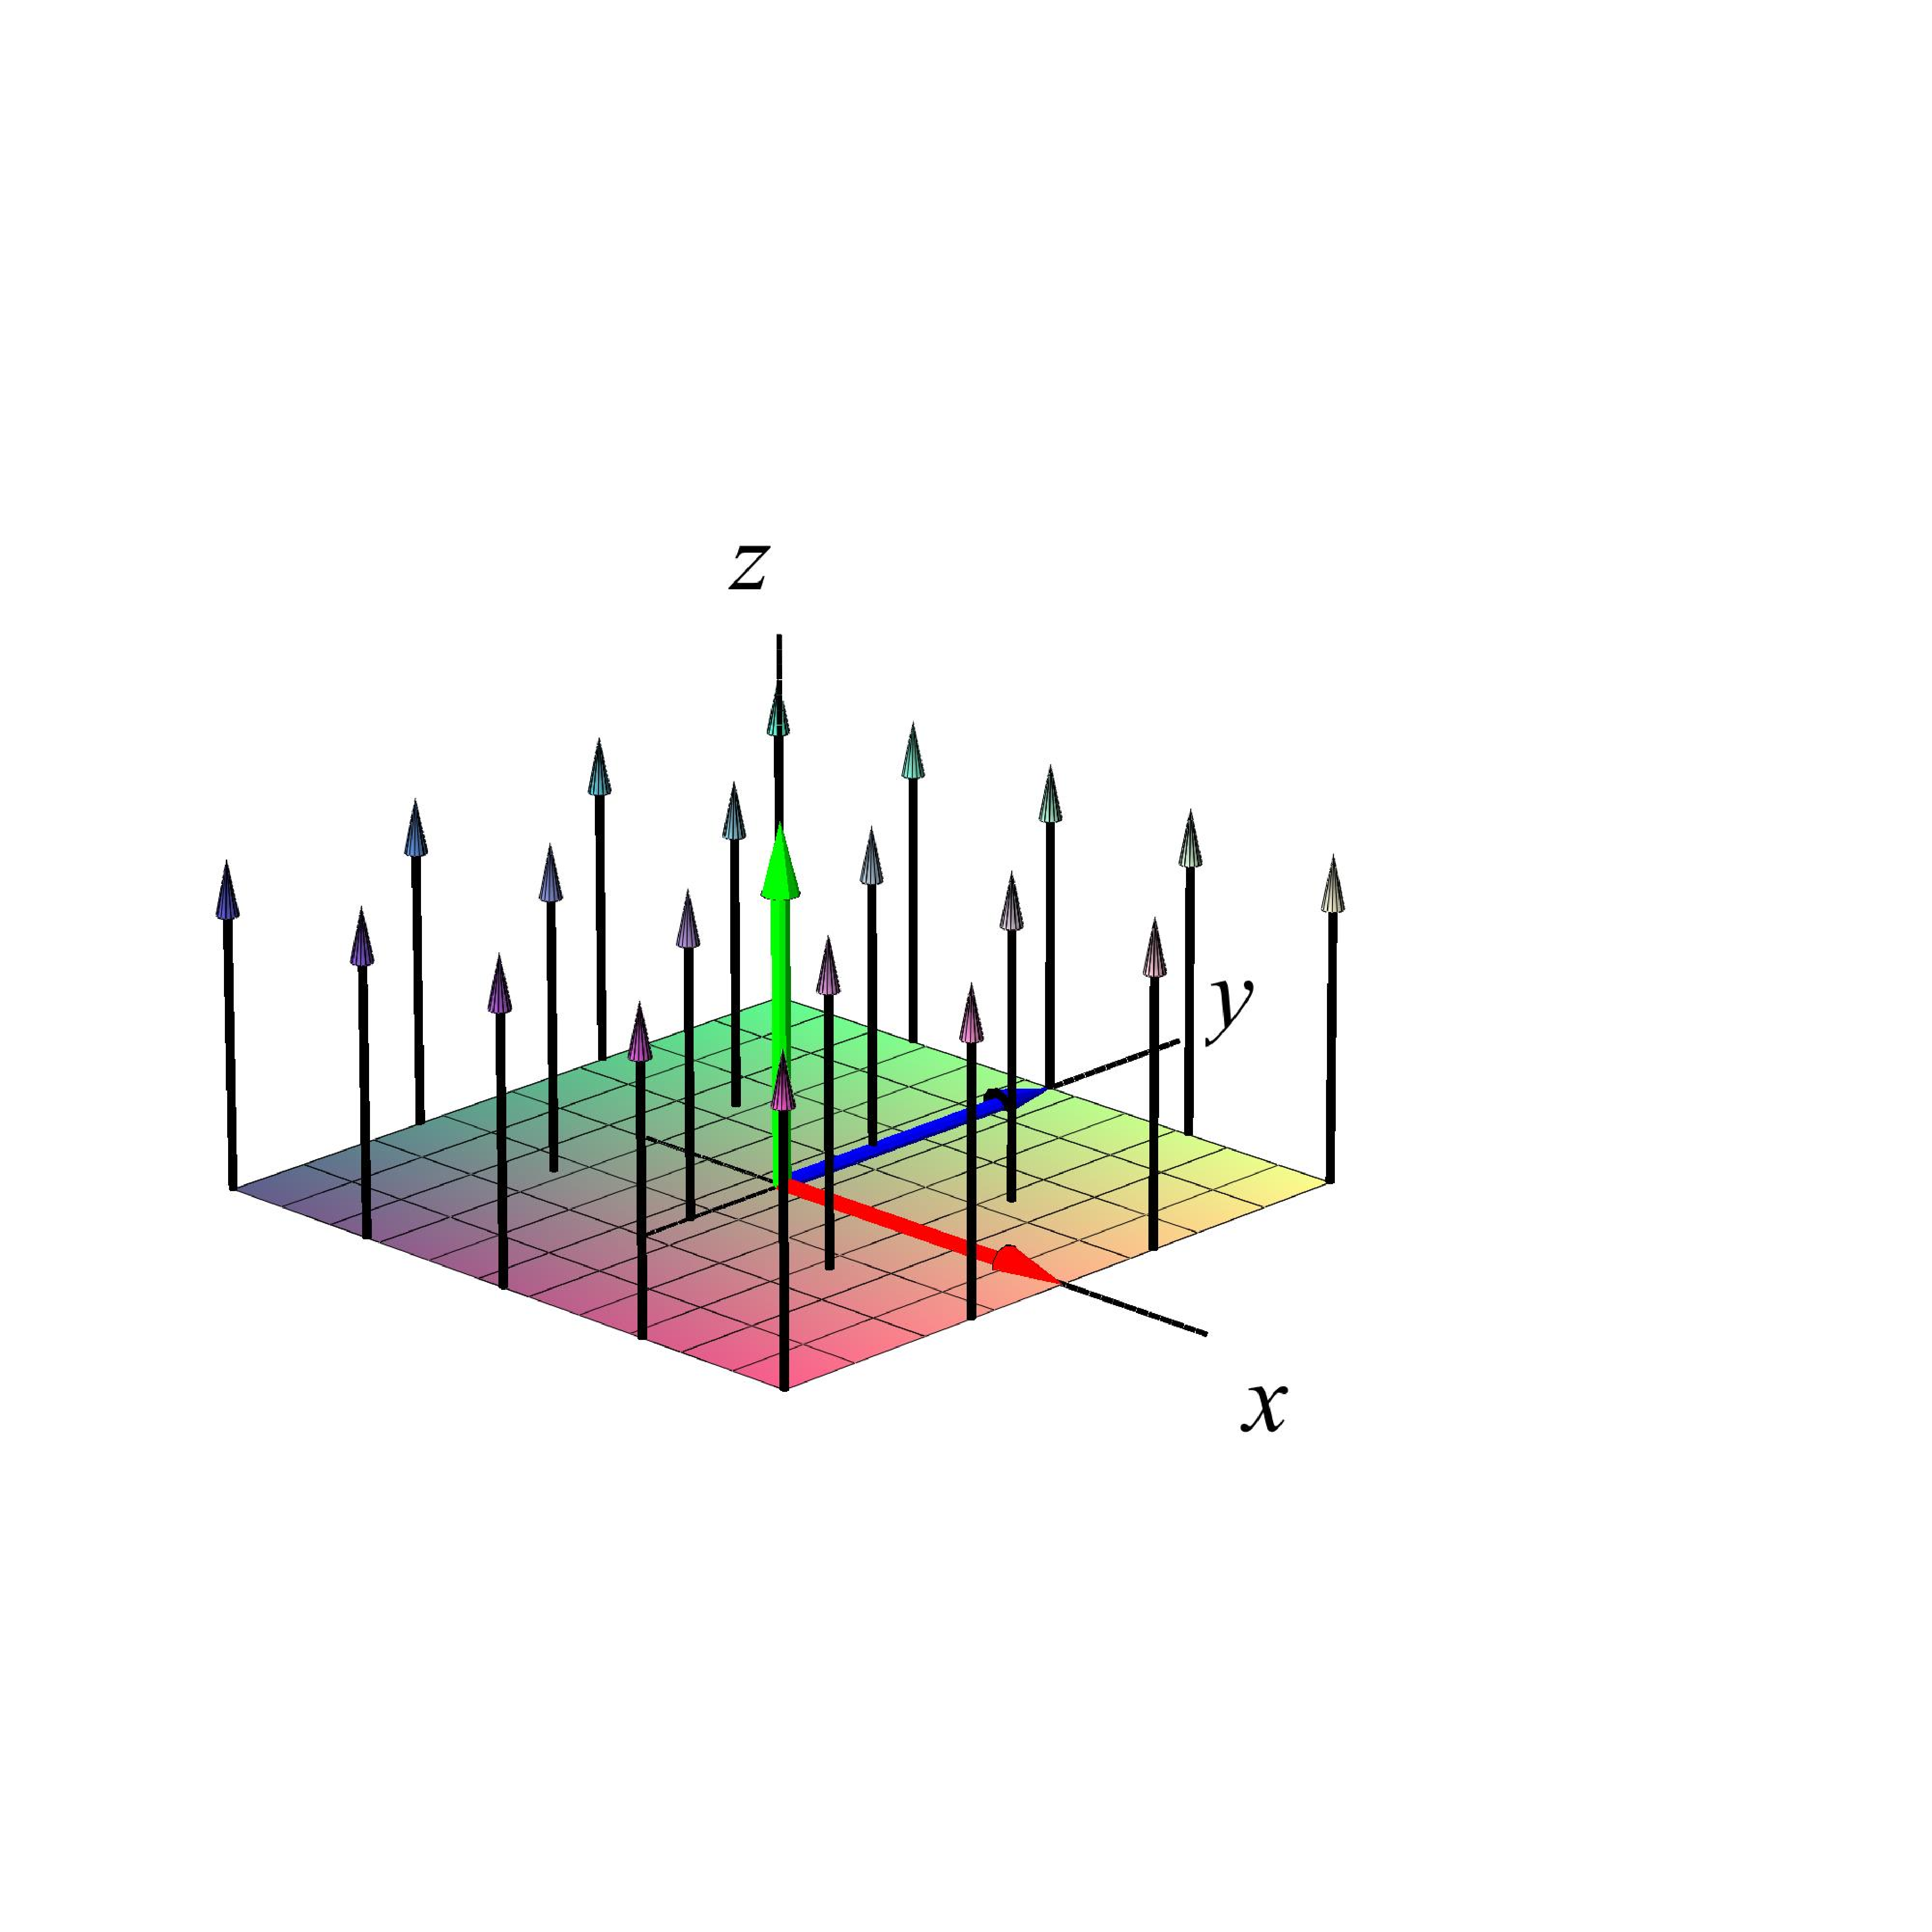
\includegraphics[height=70mm]{FIGS/plotFlat4}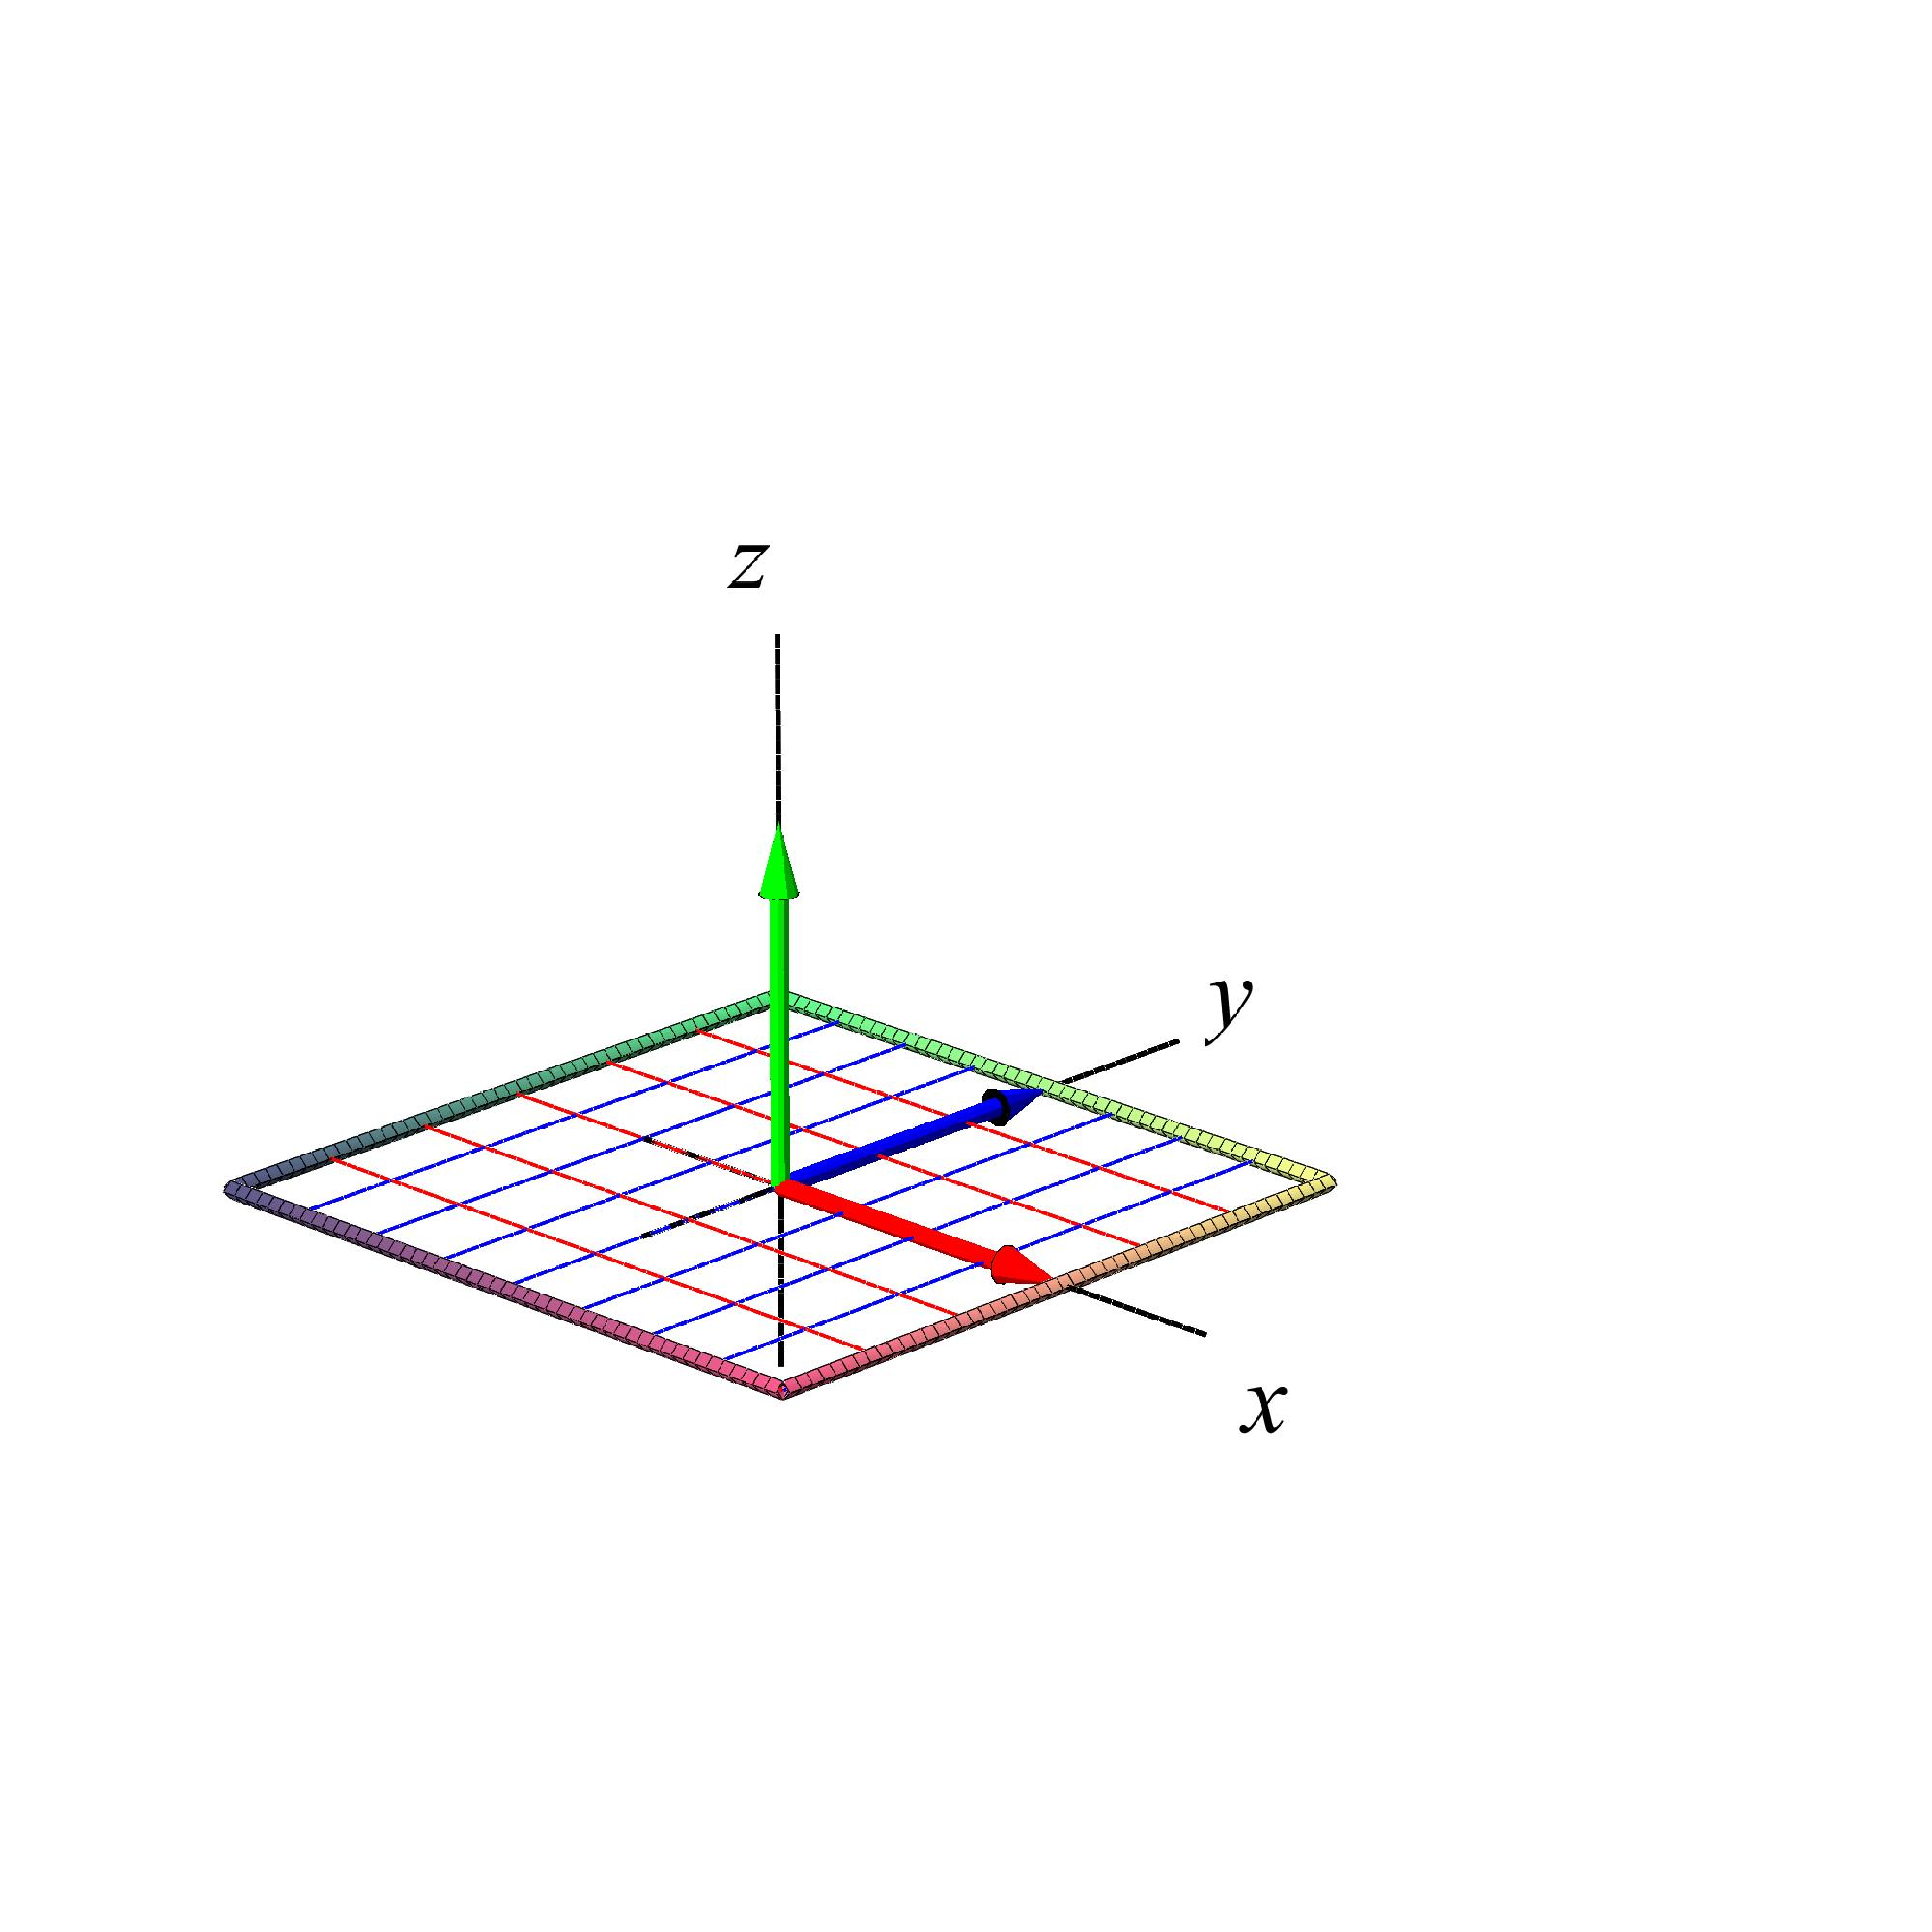
\includegraphics[height=70mm]{FIGS/plotFlat5}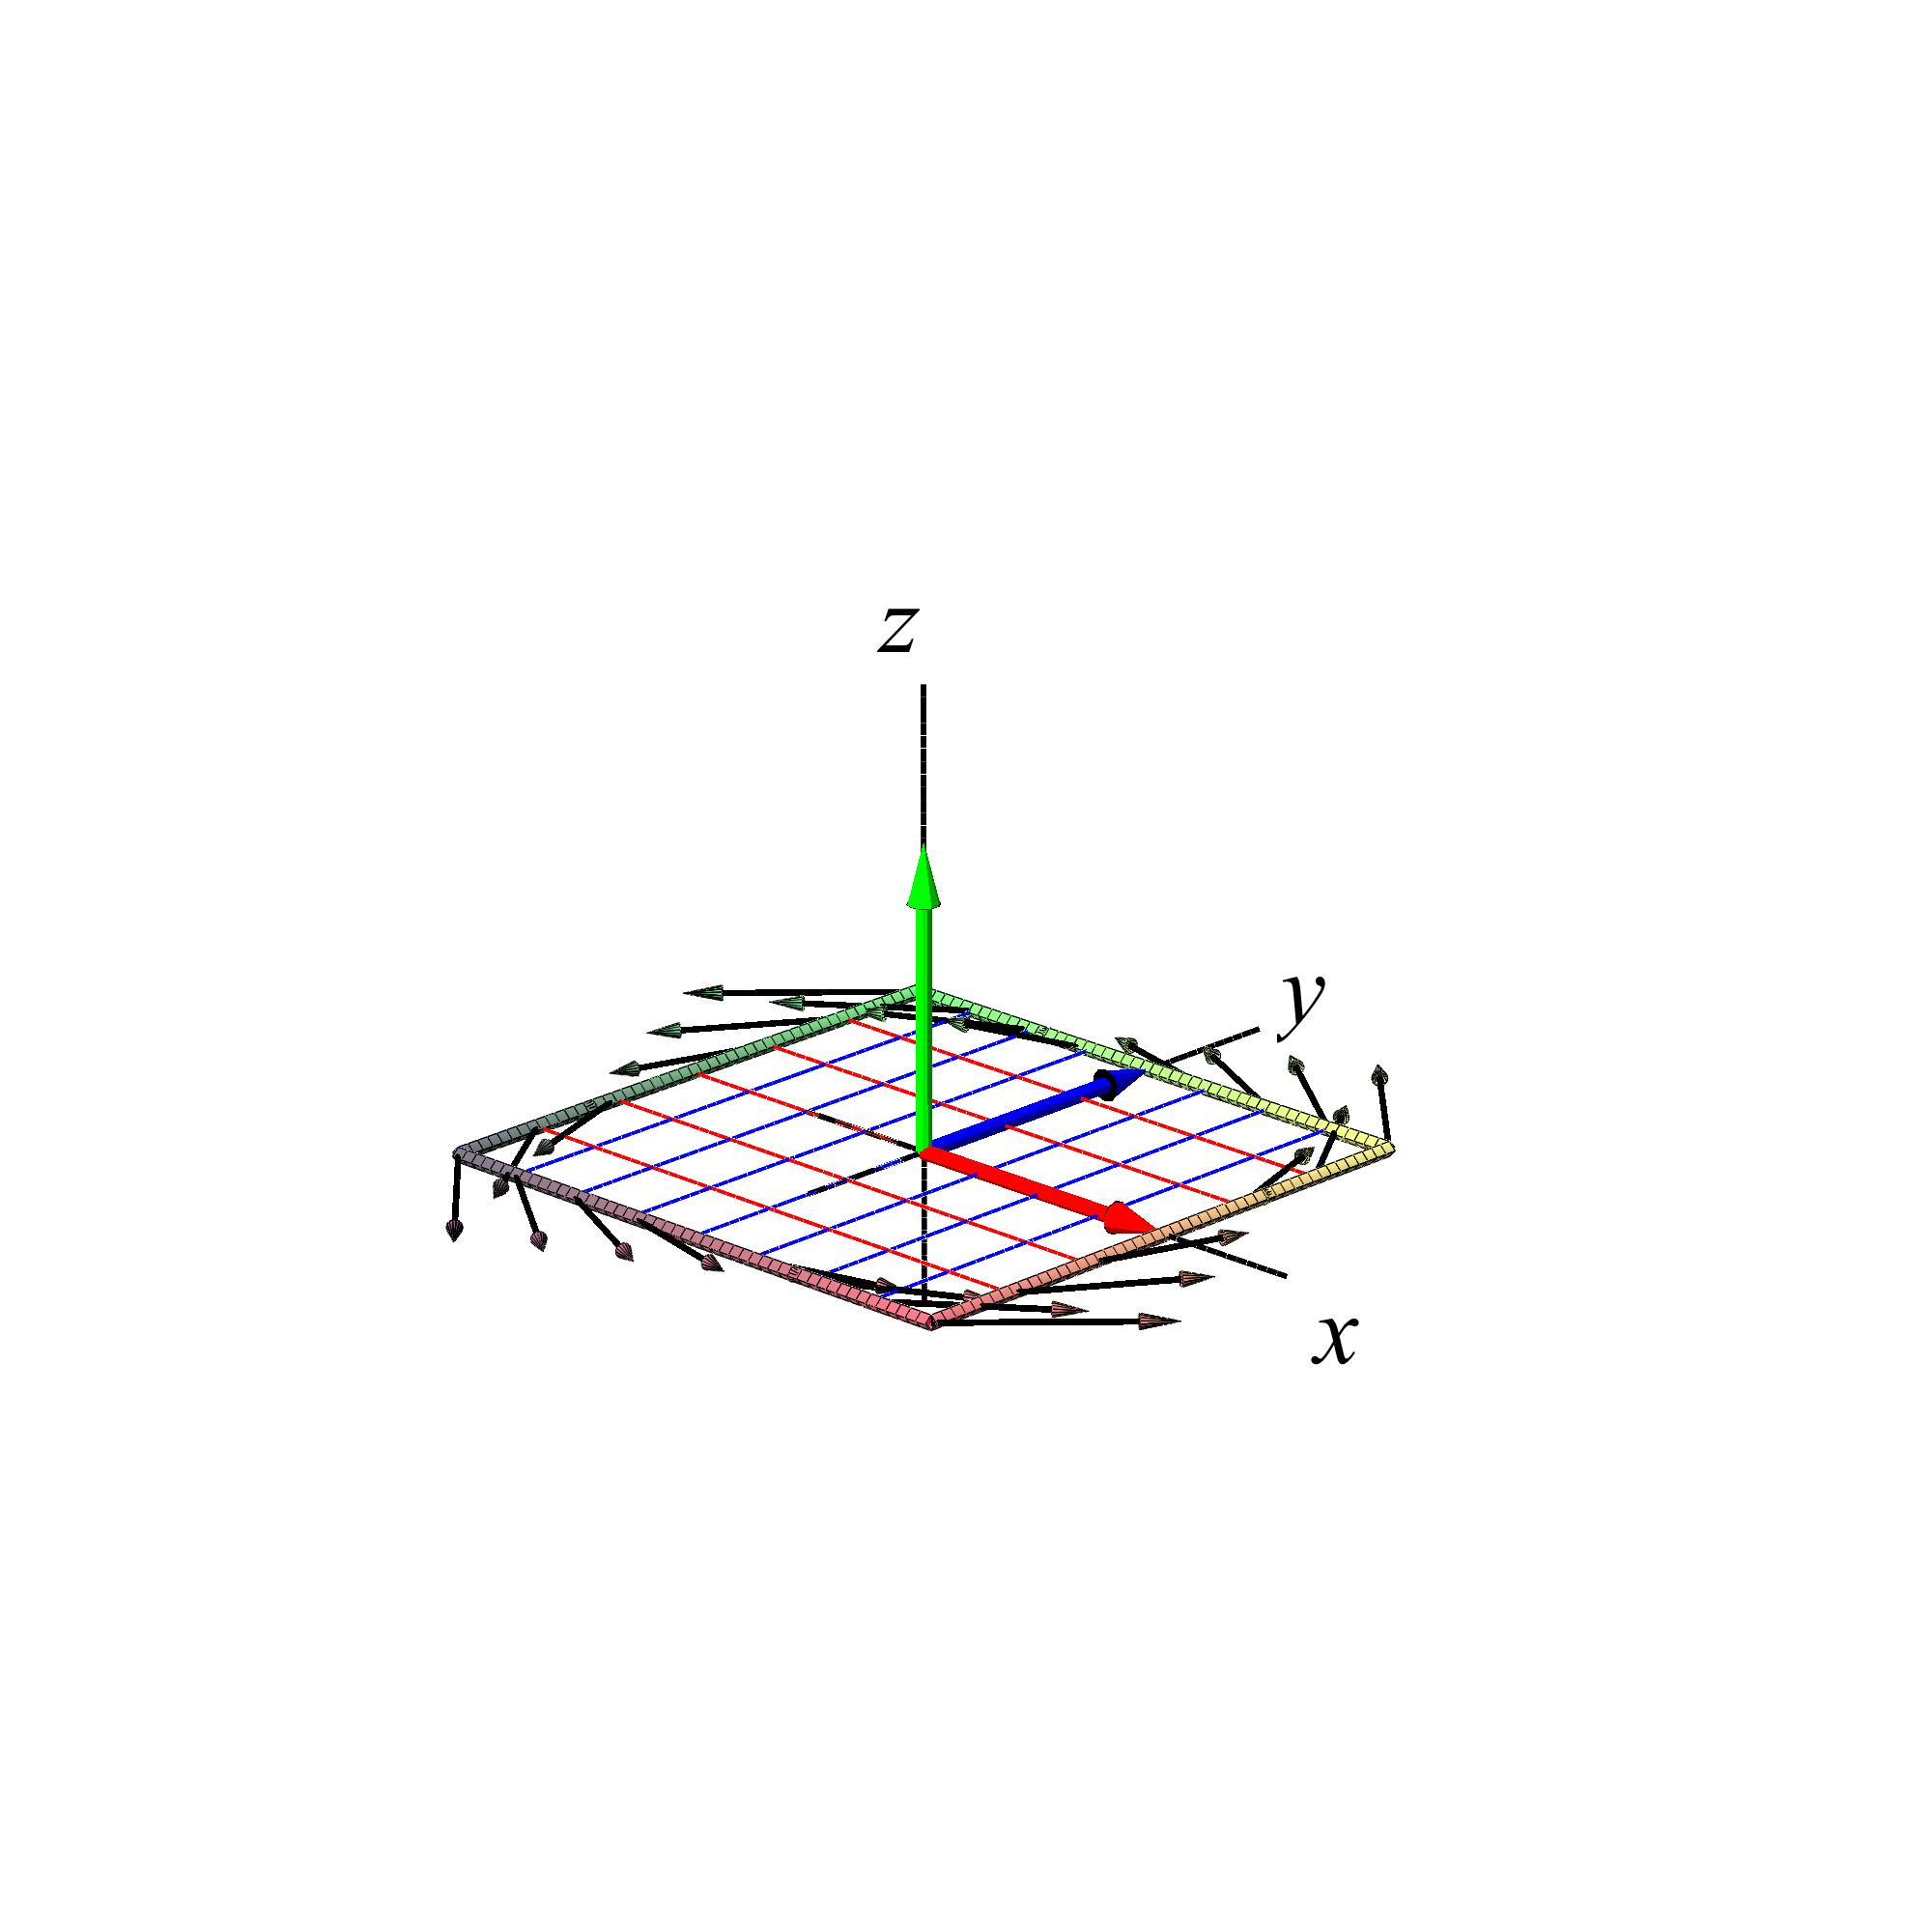
\includegraphics[height=70mm]{FIGS/plotFlat6}}
\begin{center}
\caption{\small{Opstilling af fluxen af rotationsvektorfeltet $\Rot(\mathbf{V}(x,y,z) = (0,0,2)$ igennem kvadrat i $(x,y)$-planen og tilhørende cirkulation af vektorfeltet $\mathbf{V}(x,y,z) = (-y, x, 0)$ langs den firkantede randkurve.}}
\label{figFlatStokesB}
\end{center}
\end{figure}



%%%%%%%%%%%%%%%%%%%%%%%%%%%%%%%%%%%%%%%%%%%%%%%%%%%%%%%%%%%%%
%%%%%%%%%%%%%%%%%%%%%%%%%%%%%%%%%%%%%%%%%%%%%%%%%%%%%%%%%%%%%
%%%%%%%%%%%%%%%%%%%%%%%%%%%%%%%%%%%%%%%%%%%%%%%%%%%%%%%%%%%%%

\begin{summary}
Vi har set her, at fluxen af et rotationsvektorfelt $\Rot(\mathbf{V})(x,y,z)$ igennem en flade kan beregnes som cirkulationen af $\mathbf{V}(x,y,z)$ langs randkurven til fladen -- passende orienteret.
\begin{itemize}
\item Lad $F_{\bf{r}}$ betegne en glat parametriseret flade
med randkurven $\partial F_{\bf{r}}$ og
en\-heds\--nor\-mal\-vek\-tor\-felt
$\,{\bf{n}}_{F}$ og lad ${\bf{V}}$ være et glat
vektorfelt i $\mathbb{R}^{3}$. Så udtrykker Stokes' sætning følgende identitet
\begin{equation}
\int_{F}\, \Rot({\bf{V}})\bm{\cdot} {\bf{n}}_{F} \,
\,d\mu \, = \, \int_{\partial F} \, {\bf{V}}
\bm{\cdot} {\bf{e}}_{\partial F} \, d\mu \quad .
\end{equation}
Ved beregning af højresiden er det vigtigt (for at få det korrekte fortegn) at orienteringen
af randen vælges
sådan at krydsproduktet  ${\bf{e}}_{\partial F}
\times {\bf{n}}_{F}$ peger væk fra fladen langs
med randen.
\item Alternativt kan Stokes' sætning udtrykkes således: Fluxen af \emph{rotationen af} vektorfeltet $\mathbf{V}$ igennem fladen $F_{\mathbf{r}}$ er lig med \emph{cirkulationen} af vektorfeltet
langs fladestykkets lukkede randkurve  $\partial F$:
\begin{equation}
\Flux(\Rot(\mathbf{V}), F_{\mathbf{r}}) = \operatorname{Cirk}(\mathbf{V}, \partial F) \quad .
\end{equation}
\item Den Totale rotation af et vektorfelt i et rumligt område kan tilsvarende beregnes ved fladeintegral over den totale overflade af området:  Lad $\Omega$ være et rumligt
område med randen $\partial \Omega$ og udadrettet
enheds-normalvektorfelt $\,{\bf{n}}_{\partial
\Omega}\,$ på $\partial \Omega$. Så gælder for ethvert glat vektorfelt $\mathbf{V}(x,y,z)$:
\begin{equation}
\int_{\Omega}\, \Rot({\bf{V}})\, d\mu \,  = \,
\int_{\partial \Omega}\, {\bf{n}}_{\partial
\Omega}\, \times {\bf{V}}
 \, \,d\mu \, = \, {\operatorname{\bf{Vrid}}}({\bf{V}},
\partial \Omega) \quad .
\end{equation}

\end{itemize}
\end{summary}


%%%%%%%%%%%%%%%%%%%%%%%%%%%%%%%%%%%%%%%%%%%%%
%%%%%%%%%%%%%%%%%%%%%%%%%%%%%%%%%%%%%%%%%%%%%
%%% HER SKAL DU STOPPE MED AT SKRIVE %%%%%%%%
%%%%%%%%%%%%%%%%%%%%%%%%%%%%%%%%%%%%%%%%%%%%%
%%%%%%%%%%%%%%%%%%%%%%%%%%%%%%%%%%%%%%%%%%%%%


\end{document} 

%%%%%%%%%%%%%%%%%%%%%%%%%%%%%%%%%%%%%%%%%%%%%%%%%%%
%%%%%%%%%%%%%%%%%%%%%%%%%%%%%%%%%%%%%%%%%%%%%%%%%%%

